\originalchapter{作业八至十一}
本章完整翻译公开原卷中的 15 道大题及其子问. 原卷首页署 MIT 8.962 Spring 2006, 现由 Spring 2020 OCW 资源页公开提供; 每节给出实际原件入口. 以下解答是本稿独立推导和数值计算, 不是 MIT 官方解答. 除换算题另行恢复 $G,c$ 外取 $c=1$; TOV 和黑洞轨道数值计算还取 $G=1$. 曲率号与本书约定相同. 原题的历史观测数字仅用于该题模型, 不作为当前观测更新.

\originalsection{作业八}
题源: \href{https://ocw.mit.edu/courses/8-962-general-relativity-spring-2020/resources/mit8_962s20_pset08/}{Problem Set 8, 原卷 Spring 2006, PDF 第 1--3 页}.

\begin{exercise}\label{ps:8.1}
原题 1. 领先阶引力辐射为
\[
h^{\rm TT}_{ij}=\frac{2G}{r}\ddot I_{kl}\left(P_{ik}P_{jl}-\frac12P_{ij}P_{kl}\right),\qquad
I_{kl}=\int \rho x_kx_l\,\dd V.
\]
点表示对时间求导; 在近惯性、近乎平坦的区域内不区分空间指标的升降. $P_{ij}=\delta_{ij}-n_in_j$ 投影到传播方向 $\boldsymbol n$ 的垂直平面. 证明以无迹四极矩 $\mathcal I_{kl}=I_{kl}-\delta_{kl}I/3$, $I=\delta^{kl}I_{kl}$ 替代 $I_{kl}$, 结果不变. 注意三维空间的迹与横向二维空间的迹不同. 原题还指出辐射的 $l$ 极矩一般有 $2l+1$ 个分量: 标量有一个, 偶极矩三个, 四极矩五个. 解释为何对称三维张量的六个分量中只有五个四极矩辐射分量.
\end{exercise}
\begin{solution}
$P$ 是对称幂等矩阵, $P_{ik}P_{kj}=P_{ij}$, 且 $P_{kk}=2$. 因而 TT 投影作用于三维纯迹张量时,
\[
\left(P_{ik}P_{jl}-\frac12P_{ij}P_{kl}\right)\delta_{kl}
=P_{ij}-\frac12P_{ij}\operatorname{tr}P=0.
\]
投影与时间求导交换, 所以从 $I_{kl}$ 减去 $I\delta_{kl}/3$ 不改变波形. 这里抵消使用的是 $\operatorname{tr}P=2$, 不是 $\operatorname{tr}\delta=3$; 三维去迹与二维去迹承担不同作用. 对称 $3\times3$ 张量有六个独立分量, 三维迹占其中一个, 剩余五个构成 $l=2$ 的无迹对称表示. 固定一个传播方向后再施加横向条件, 波形只剩两个偏振; ``五个源四极矩分量'' 与 ``两个远区偏振'' 并不矛盾.
\end{solution}

\begin{exercise}\label{ps:8.2}
原题 2. 两质量 $m_1,m_2$ 组成牛顿圆轨道双星, 相对轨道半径为 $R$. 采用约化系统: $M=m_1+m_2$, $\mu=m_1m_2/M$.
\begin{enumerate}[label=(\alph*)]
\item 从轨道角动量轴方向观测, 求 $h^{\rm TT}_{ij}$.
\item 求引力波带走能量的速率.
\item 由 $\dd(E_{\rm kin}+E_{\rm pot}+E_{\rm GW})/\dd t=0$ 推导轨道半径的收缩率 $\dot r$.
\item 求轨道角频率 $\dot\Omega$. 证明质量只通过啁啾质量 $\mathcal M=\mu^{3/5}M^{2/5}$ 出现.
\end{enumerate}
\end{exercise}
\begin{solution}
(a) 以质心为原点, 相对位矢为 $\boldsymbol x=r(\cos\Omega t,\sin\Omega t,0)$. 两物体的质量二阶矩之和恰为 $I_{ij}=\mu x_ix_j$; 此处 $r=R$ 是两星间距, 不是某一颗星到质心的距离. 令观测距离为 $D$ 以免与轨道半径混淆, 则
\[
I_{xx}=\frac{\mu r^2}{2}(1+\cos2\Omega t),\quad
I_{yy}=\frac{\mu r^2}{2}(1-\cos2\Omega t),\quad
I_{xy}=\frac{\mu r^2}{2}\sin2\Omega t.
\]
沿 $z$ 轴投影后 $\ddot I_{xx}+\ddot I_{yy}=0$, 所以
\[
h^{\rm TT}_{ij}=-\frac{4G\mu r^2\Omega^2}{D}
\begin{pmatrix}\cos2\Omega t&\sin2\Omega t&0\\
\sin2\Omega t&-\cos2\Omega t&0\\0&0&0\end{pmatrix}.
\]
整体相位由时间原点决定, 辐射角频率是轨道角频率的两倍.

(b) 应对全部立体角积分, 不能把轴向的通量乘 $4\pi D^2$ 代替总功率. 由四极矩公式
\[
\mathcal P=\frac G5\left\langle\dddot{\mathcal I}_{ij}\dddot{\mathcal I}_{ij}\right\rangle
\]
计算. 三维迹 $\mu r^2$ 是常数, 不影响三阶导数; 两个对角分量的振幅为 $4\mu r^2\Omega^3$, 两个非对角分量亦然, 于是缩并为 $32\mu^2r^4\Omega^6$. 因此
\[
\mathcal P=\frac{32}{5}G\mu^2r^4\Omega^6
=\frac{32}{5}\frac{G^4\mu^2M^3}{r^5},\qquad \Omega^2=\frac{GM}{r^3}.
\]
(c) 牛顿圆轨道能量是 $E_{\rm orb}=-G\mu M/(2r)$. 采用缓慢变化的准圆轨道, 能量平衡给出
\[
\frac{G\mu M}{2r^2}\dot r=-\mathcal P,
\qquad \dot r=-\frac{64}{5}\frac{G^3\mu M^2}{r^3}.
\]
这是一阶耗散近似, 接近强场并合时已不适用.

(d) 从 Kepler 关系取导数, $\dot\Omega=-3\Omega\dot r/(2r)$, 代入上式并以 $r=(GM/\Omega^2)^{1/3}$ 消去半径, 得
\[
\dot\Omega=\frac{96}{5}G^{5/3}\mu M^{2/3}\Omega^{11/3}
=\frac{96}{5}(G\mathcal M)^{5/3}\Omega^{11/3}.
\]
恢复单位时, 波形乘 $c^{-4}$, 功率与收缩率乘 $c^{-5}$, 最后式写成 $(96/5)(G\mathcal M/c^3)^{5/3}\Omega^{11/3}$. 质量较大的系统在相同频率处啁啾更快.
\end{solution}

\begin{exercise}\label{ps:8.3}
原题 3. 在线性化理论中建立 Riemann 张量的波动方程. 设 $g_{\mu\nu}=\eta_{\mu\nu}+h_{\mu\nu}$, $\|h\|\ll1$, 且 $R_{\alpha\beta}=8\pi G\bar T_{\alpha\beta}$, $\bar T_{\alpha\beta}=T_{\alpha\beta}-g_{\alpha\beta}T/2$.
\begin{enumerate}[label=(\alph*)]
\item 用线性 Bianchi 恒等式 $\partial_\alpha R_{\beta\gamma\mu\nu}+\partial_\beta R_{\gamma\alpha\mu\nu}+\partial_\gamma R_{\alpha\beta\mu\nu}=0$, 求 $\partial_\alpha R^\alpha{}_{\beta\gamma\delta}$ 与 $\bar T$ 的梯度的关系.
\item 推导 $\Box R_{\alpha\beta\mu\nu}$ 的二阶导数源, 用推迟 Green 函数给形式解.
\item 真空中沿 $z$ 传播的平面波满足 $R_{\alpha\beta\mu\nu}=R_{\alpha\beta\mu\nu}(t-z)$. 用 Bianchi 恒等式和曲率对称性说明其独立非零分量可以用 $R_{i0j0}$ 表示. 原题称其他分量 ``由对称性平凡相关'', 解答须说明含 $z$ 的关联.
\item 证明其中只需 $R_{x0x0}=-R_{y0y0}$ 与 $R_{x0y0}=R_{y0x0}$, 分别对应 $+$ 与 $\times$ 偏振.
\item 定义 $R_{x0x0}=-\partial_t^2h_+/2$, $R_{x0y0}=-\partial_t^2h_\times/2$. 比较
\[
R_{\alpha\beta\mu\nu}=\frac12(\partial_\alpha\partial_\nu h_{\beta\mu}+\partial_\beta\partial_\mu h_{\alpha\nu}-\partial_\alpha\partial_\mu h_{\beta\nu}-\partial_\beta\partial_\nu h_{\alpha\mu})
\]
与上述表达式, 证明 $h_+=h^{\rm TT}_{xx}=-h^{\rm TT}_{yy}$, $h_\times=h^{\rm TT}_{xy}=h^{\rm TT}_{yx}$.
\item 绕 $z$ 轴转动坐标, $x'+iy'=(x+iy)e^{-i\theta}$. 证明 $h'_++ih'_\times=(h_++ih_\times)e^{-2i\theta}$, 并解释自旋权重 2.
\end{enumerate}
\end{exercise}
\begin{solution}
(a) 对 Bianchi 恒等式缩并一对指标, 利用 $R_{abcd}=-R_{bacd}=-R_{abdc}=R_{cdab}$, 得
\[
\partial^aR_{abcd}=\partial_cR_{bd}-\partial_dR_{bc}
=8\pi G(\partial_c\bar T_{bd}-\partial_d\bar T_{bc}).
\]
这里缩并的是时空指标, 升降用 $\eta$, 不可以用三维 $\delta$ 代替.

(b) 在 $\partial_eR_{abcd}+\partial_cR_{abde}+\partial_dR_{abec}=0$ 上作用 $\partial^e$, 再用 (a), 得
\begin{align*}
\Box R_{abcd}=8\pi G S_{abcd},\qquad
S_{abcd}={}&\partial_c\partial_a\bar T_{bd}-\partial_c\partial_b\bar T_{ad}\\
&-\partial_d\partial_a\bar T_{bc}+\partial_d\partial_b\bar T_{ac}.
\end{align*}
在 $(-+++)$ 下 $\Box=-\partial_t^2+\nabla^2$. 若 $\Box G_{\rm ret}=\delta^{(4)}$, 则 $G_{\rm ret}(t,\boldsymbol x)=-\delta(t-|\boldsymbol x|)/(4\pi|\boldsymbol x|)$, 形式解为
\[
R_{abcd}(x)=R^{\rm hom}_{abcd}(x)+8\pi G\int G_{\rm ret}(x-x')S_{abcd}(x')\,\dd^4x'.
\]
$R^{\rm hom}$ 携带初始自由波; 选无入射辐射边界条件时取相应推迟解. 源的微分在积分中对 $x'$ 作用, 不得忽略 Green 函数的支持条件.

(c) 令 $u=t-z$, $k_a=\partial_a u=(1,0,0,-1)$, $A,B\in\{x,y\}$. 对非恒定的辐射部分, Bianchi 恒等式变成 $k_{[e}R'_{ab]cd}=0$. 积分常数若非零代表额外静态背景, 本题平面辐射条件将其排除. 取 $e=0$、$a=x$、$b=y$, 得 $R_{xycd}=0$. 再取 $e=0$、$a=z$、$b=A$, 得 $R_{zAcd}=-R_{0Acd}$. 用两对指标交换, 相同关系也适用于后一对. 真空散度式 $k^aR_{abcd}=0$ 进一步给 $R_{0zcd}=0$. 因此每一对反对称指标只需一个横向指标和一个 $0$ 或 $z$, 并有
\[
R_{A0B0}=C_{AB},\qquad R_{A0Bz}=-C_{AB},\qquad R_{AzBz}=C_{AB}.
\]
故含 $z$ 的分量一般并非零; 它们除曲率指标对称性外, 还通过 Bianchi 恒等式与传播关系确定. 这是对原题措辞所必需的补充.

(d) 两对指标交换给 $C_{AB}=C_{BA}$. 真空 $R_{00}=0$ 给 $C_{xx}+C_{yy}=0$, 而带 $z$ 的潮汐分量已经消失. 从而
\[
C_{AB}=\begin{pmatrix}C_+&C_\times\\C_\times&-C_+\end{pmatrix},
\]
只剩两个任意函数.

(e) TT 规范中 $h_{0a}=h_{za}=0$, 故线性曲率式直接给 $R_{A0B0}=-\ddot h^{\rm TT}_{AB}/2$. 比较定义即得所求. 两次积分允许加上线性时间函数和常数, 它们不产生该曲率; 固定无非辐射背景的边界条件后可将其置零.

(f) 令 $c_\theta=\cos\theta$, $s_\theta=\sin\theta$. 坐标变换矩阵为 $Q=\left(\begin{smallmatrix}c_\theta&s_\theta\\-s_\theta&c_\theta\end{smallmatrix}\right)$, 所以横向张量变成 $h'=QhQ^{\mathsf T}$. 逐项相乘得到
\[
h'_+=h_+\cos2\theta+h_\times\sin2\theta,\qquad
h'_\times=-h_+\sin2\theta+h_\times\cos2\theta.
\]
合并为复数即为原题等式. 旋转角出现两倍, 描述的是横向二阶无迹张量的自旋权重; 它不是说经典波形存在两倍的空间旋转频率.
\end{solution}

\begin{exercise}\label{ps:8.4}
原题 4. 从完整 Bianchi 恒等式 $\nabla_\alpha R_{\beta\gamma\mu\nu}+\nabla_\beta R_{\gamma\alpha\mu\nu}+\nabla_\gamma R_{\alpha\beta\mu\nu}=0$ 出发.
\begin{enumerate}[label=(\alph*)]
\item 给出上一题 (a) 的完全协变形式.
\item 推导 $\Box R^\alpha{}_{\beta\gamma\delta}$ 的非线性波动方程, $\Box=\nabla^\mu\nabla_\mu$. 源须包含 $\bar T$ 的双协变梯度、$\bar T$ 与曲率耦合、曲率与曲率耦合三类项. 这是常称 Penrose 波动方程的一种形式; 原题注明该非线性波动方程由 Roger Penrose 首先建立; Teukolsky 在黑洞曲率背景附近展开所发展的变体在天体相对论研究中十分重要.
\end{enumerate}
\end{exercise}
\begin{solution}
(a) 度规相容 $\nabla g=0$, 因此前一题的缩并不变,
\[
\nabla^aR_{abcd}=\nabla_cR_{bd}-\nabla_dR_{bc}
=8\pi G(\nabla_c\bar T_{bd}-\nabla_d\bar T_{bc}).
\]
(b) 非线性的来源正是协变导数不能交换. 先保持交换子, 这样每个符号均可追查:
\begin{align*}
\Box R_{abcd}={}&\nabla_c\nabla_aR_{bd}-\nabla_c\nabla_bR_{ad}
-\nabla_d\nabla_aR_{bc}+\nabla_d\nabla_bR_{ac}\\
&-g^{ef}\bigl([\nabla_f,\nabla_c]R_{abde}+[\nabla_f,\nabla_d]R_{abec}\bigr).
\end{align*}
它由末三指标 Bianchi 恒等式取散度获得. 对任意四阶全协变张量 $A$, 本书曲率号下
\[
[\nabla_f,\nabla_c]A_{abde}
=-R^h{}_{afc}A_{hbde}-R^h{}_{bfc}A_{ahde}
-R^h{}_{dfc}A_{abhe}-R^h{}_{efc}A_{abdh}.
\]
将 $A=R$ 代入, 用 $g^{ef}R^h{}_{efc}=-R^h{}_c$, 即可把两项交换子展开成
\begin{align*}
\Box R_{abcd}={}&8\pi G\bigl(\nabla_c\nabla_a\bar T_{bd}-\nabla_c\nabla_b\bar T_{ad}
-\nabla_d\nabla_a\bar T_{bc}+\nabla_d\nabla_b\bar T_{ac}\bigr)\\
&+8\pi G\bigl(\bar T^h{}_cR_{abhd}+\bar T^h{}_dR_{abch}\bigr)+Q_{abcd},
\end{align*}
其中完全写出的二次曲率项为
\begin{align*}
Q_{abcd}=g^{ef}\bigl(&R^h{}_{afc}R_{hbde}+R^h{}_{bfc}R_{ahde}+R^h{}_{dfc}R_{abhe}\\
&+R^h{}_{afd}R_{hbec}+R^h{}_{bfd}R_{ahec}+R^h{}_{cfd}R_{abeh}\bigr).
\end{align*}
最后用 $g^{a\alpha}$ 升起首指标即可得到题目所需形式, 因为 $\nabla g=0$, 升指标与 $\Box$ 交换. 真空仍有 $Q$, 说明曲率能够自耦合; 在线性化极限, $Q$ 和 $\bar T R$ 都是二阶小量, 协变导数变为偏导, 恰好恢复上一题. 此处没有引入额外的 $8\pi G$ 乘在纯几何 $Q$ 前; 若把所有项统称为题面的 ``源'', 该项在括号内应除以 $8\pi G$.
\end{solution}

\originalsection{作业九}
题源: \href{https://ocw.mit.edu/courses/8-962-general-relativity-spring-2020/resources/mit8_962s20_pset09/}{Problem Set 9, 原卷 Spring 2006, PDF 第 1--4 页}.

\begin{exercise}\label{ps:9.1}
原题 1. 微引力透镜中两像不能分辨, 只能观测两像总亮度. 源星在大麦哲伦云, 原题取距离约 $100\,\mathrm{kpc}$; 银河系内不可见透镜的质量约为一个太阳质量、距离约 $10\,\mathrm{kpc}$, 轨道速率约 $200\,\mathrm{km/s}$. 给定 $1\,\mathrm{pc}=3.26$ 光年 $=3.1\times10^{13}\,\mathrm{km}$, 估计亮度先增后减的变化时间尺度. 原题以 4 月 20 日课堂、Hartle 第 11 章作为背景.
\end{exercise}
\begin{solution}
弱场点质量透镜的物理 Einstein 半径满足
\[
R_E^2=\frac{4GM}{c^2}\frac{D_LD_{LS}}{D_S}.
\]
透镜横穿约一个 $R_E$ 时放大率发生显著变化, 因而 $t_E=R_E/v_\perp$. 本题 $D_LD_{LS}/D_S=9\,\mathrm{kpc}=2.79\times10^{17}\,\mathrm{km}$, $GM_\odot/c^2\simeq1.477\,\mathrm{km}$, 得 $R_E\simeq1.28\times10^9\,\mathrm{km}$, 约 $8.6\,\mathrm{AU}$. 于是 $t_E\simeq6.4\times10^6\,\mathrm{s}\simeq74$ 天. 若把显著增亮至变暗的全宽取为穿越直径, 则约 $2t_E\simeq148$ 天. 具体半高宽还依赖最小冲量参数, 题给数据足以判断其量级为数月, 不能唯一确定完整光变曲线宽度.
\end{solution}

\begin{exercise}\label{ps:9.2}
原题 2. 采用 Carroll 式 (8.124) 的自行距离定义计算 $d_M(z)$, 并核实
\[
d_L(z)=(1+z)d_M(z)=(1+z)^2d_A(z).
\]
这里 $d_L$ 为光度距离, $d_A$ 为角直径距离. 题目希望结果与该书式 (8.123) 的形式一致.
\end{exercise}
\begin{solution}
自行距离的操作定义是: 源的横向本征速率 $v_\perp$ 与观测角速度 $\mu_{\rm ang}=\dd\theta/\dd t_0$ 满足 $v_\perp=\mu_{\rm ang}d_M$. 这一定义包含源钟与观测钟的时间膨胀. 写 FRW 度规为
\[
\dd s^2=-\dd t^2+a(t)^2[\dd\chi^2+S_k(\chi)^2\dd\Omega^2],
\]
其中 $S_k(\chi)=\sin\chi,\chi,\sinh\chi$ 分别对应 $k=1,0,-1$; 若 $\chi$ 带长度维度, 正负曲率时相应插入曲率半径. 源处横向位移是 $v_\perp\dd t_e=a_eS_k(\chi)\dd\theta$, 而 $\dd t_0=(1+z)\dd t_e$, 因此
\[
d_M=(1+z)a_eS_k(\chi)=a_0S_k(\chi),\qquad
\chi(z)=\frac1{a_0}\int_0^z\frac{\dd z'}{H(z')}.
\]
这是一般膨胀史的答案; 未给物质组成时不能替换成某个特定 $H(z)$. 如以现今曲率参数 $\Omega_{k0}$ 表示并恢复 $c$, 令 $E(z)=H(z)/H_0$, 则
\[
d_M=\frac{c}{H_0\sqrt{|\Omega_{k0}|}}\,\mathcal{S}\!\left(\sqrt{|\Omega_{k0}|}\int_0^z\frac{\dd z'}{E(z')}\right),
\]
$\Omega_{k0}>0$ 时 $\mathcal S=\sinh$, $\Omega_{k0}<0$ 时 $\mathcal S=\sin$; 平坦极限为 $(c/H_0)\int\dd z'/E$. 又 $d_A=a_eS_k(\chi)$, 光子能量和到达率各红移一次, $F=L/[4\pi a_0^2S_k^2(1+z)^2]$, 故 $d_L=(1+z)a_0S_k(\chi)$, 得到全部距离关系. 该关系以光子数守恒和度规光传播为条件.
\end{solution}

\begin{exercise}\label{ps:9.3}
原题 3. 早期热等离子体使光子反复散射; 复合后电子、质子形成原子, 光子自由传播, 留下 CMB. 原题取复合红移 $z_r\simeq1200$, 温度各向异性约 $10^{-5}$. 考虑 $k=0$ FRW 宇宙, 复合前辐射主导, 之后物质主导. $r_H(t_r)$ 是从大爆炸至复合时光子可走的最大共动距离, $r_{\rm obs}(t_r)$ 是复合至今日的共动距离.
\begin{enumerate}[label=(\alph*)]
\item 计算 $r_H$ 和 $r_{\rm obs}$.
\item 为何 $r_H/r_{\rm obs}$ 很小却有近乎各向同性 CMB 构成视界问题?
\item 求今日角间距阈值 $\theta_c$, 小于它的源在复合前可相互因果联系, 大于它的源不能.
\end{enumerate}
原题近似把物质--辐射相等时刻取为复合时刻, 同时注明实际相等红移约 3000, 只追求量级. 后两题共用 $T_0=2.73\,\mathrm K$, $k_B=8.6\times10^{-11}\,\mathrm{MeV/K}$, $\hbar=6.6\times10^{-22}\,\mathrm{MeV\,s}$,
$\sigma=\pi^2k_B^4/(60\hbar^3c^2)$, 光子气体能量密度 $u=4\sigma T^4/c$. 忽略中微子等相对论组分. 早期温度为 $(1+z)T_0$; 原卷该温度句中的尺度因子分子、分母次序有笔误.
\end{exercise}
\begin{solution}
(a) 令 $a_0=1$, $a_r=(1+z_r)^{-1}$, $H_r=H(t_r)$. 为使突变模型仍满足同一 Friedmann 初值, 在过渡处让 $a,H$ 连续. 辐射阶段有 $a=a_r(t/t_r)^{1/2}$, $H_r=1/(2t_r)$; 物质阶段则有
\[
a=a_r\left(1+\frac32H_r(t-t_r)\right)^{2/3},\quad
H(a)=H_r(a_r/a)^{3/2}.
\]
后一个幂律的时间原点有平移, 不能同时强行写成同一原点的 $t^{1/2}$ 和 $t^{2/3}$ 而又要求 $H$ 连续. 径向零线满足 $\dd\chi=\dd t/a$, 故
\[
r_H=\int_0^{t_r}\frac{\dd t}{a(t)}=\frac{2t_r}{a_r}=\frac1{a_rH_r},\qquad
r_{\rm obs}=\int_{a_r}^{1}\frac{\dd a}{a^2H(a)}=
\frac{2}{a_rH_r}\bigl(\sqrt{1+z_r}-1\bigr).
\]
于是 $r_H/r_{\rm obs}=1/[2(\sqrt{1201}-1)]=0.01486$. 绝对距离还需要 $H_r$ 或 $H_0$; 在此模型中亦可写 $r_H=1/(H_0\sqrt{1201})$, $r_{\rm obs}=2H_0^{-1}(1-1201^{-1/2})$. 恢复距离单位时两式乘 $c$.

(b) 相反方向 CMB 的共动间距为 $2r_{\rm obs}\gg r_H$. 普通辐射、物质膨胀史不允许这些区域在复合前交换信号, 却要求初始温度在约 $10^{-5}$ 精度下几乎一致. 这说明该膨胀史本身没有提供使远隔区域热平衡的机制, 而不是证明均匀初始条件逻辑上不可能.

(c) 两方向在复合球上的弦长为 $d=2r_{\rm obs}\sin(\theta/2)$. 按题面 ``彼此发送信号可达'' 的条件 $d\le r_H$, 得
\[
\theta_c=2\arcsin\frac{r_H}{2r_{\rm obs}}\simeq0.01486\,\mathrm{rad}=0.851^\circ.
\]
若要求的只是两处拥有重叠的过去光锥, 条件为 $d\le2r_H$, 角度约加倍. 若不用 $H$ 连续而把两幂律粗略接于同一时间原点, 则得到约 $1.13^\circ$ 的系数; 原题的量级结论均为约一度, 本稿后题统一使用上述连续模型.
\end{solution}

\begin{exercise}\label{ps:9.4}
原题 4. 极早期 $t_1\le t\le t_2\ll t_r$ 宇宙处于假真空, 标量场的势近似常数 $\rho_{\rm vac}\simeq V(\phi)$, 等效宇宙学常数 $\Lambda=8\pi\rho_{\rm vac}$. 以 $u_{\rm vac}\simeq(4\sigma/c)T_{\rm vac}^4$, $k_BT_{\rm vac}\sim10^{15}\,\mathrm{GeV}$ 表示其能标; 这不表示真空真的有光子气体温度. $t_2$ 左右标量场衰变为普通粒子, 此后先辐射主导、再物质主导. 取 $V$ 在该区间不变、$t>t_2$ 后近似为零.
\begin{enumerate}[label=(\alph*)]
\item 恢复 $G,c$, 利用 $1\,\mathrm{MeV}=1.6\times10^{-12}\,\mathrm{g\,cm^2/s^2}$, 求以 $\mathrm{s^{-2}}$ 表示的 $\Lambda$.
\item 重算上一题的两个距离, 求令 $r_{\rm obs}/r_H=1$ 的 $N_e=(t_2-t_1)\sqrt{\Lambda/3}$, 并取 $t_1\simeq0$ 估计 $t_2$.
\item 求暴胀期间的膨胀倍数 $a(t_2)/a(t_1)$.
\item 重算因果联系的角尺度 $\theta_c$.
\end{enumerate}
\end{exercise}
\begin{solution}
(a) 当 $\rho$ 表示能量密度时, 时间单位的宇宙学常数是 $\Lambda_t=8\pi Gu_{\rm vac}/c^2$; 空间单位的常数则是 $\Lambda_t/c^2$. 用给定光子式作能标换算,
\[
u_{\rm vac}=\frac{\pi^2}{15}\frac{(k_BT_{\rm vac})^4}{\hbar^3c^3}.
\]
取 $k_BT_{\rm vac}=10^{18}\,\mathrm{MeV}$, 把最后的 MeV 转为 erg, 得
$\Lambda_t\simeq2.54\times10^{65}\,\mathrm{s^{-2}}$, $H_I=\sqrt{\Lambda_t/3}\simeq2.91\times10^{32}\,\mathrm{s^{-1}}$. 只有能标估计准确到量级, 下列有效数字便于复算而不表示真实暴胀参数如此确定.

(b) 暴胀阶段 $a=a_2e^{H_I(t-t_2)}$, 所以此阶段对共动视界的贡献为
\[
\int_{t_1}^{t_2}\frac{\dd t}{a}=
\frac{e^{N_e}-1}{H_Ia_2}.
\]
原题没有给暴胀前的膨胀史. 为完成其 $t_1\simeq0$ 估计, 取该段更早贡献可忽略, 并设瞬时再热能标为 $T_{\rm vac}$. 这两个模型假设都影响精确 $N_e$. 以 $a_2=T_0/T_{\rm vac}$, $\alpha=a_2/a_r$ 表示, 辐射阶段 $H_ra_r^2=H_Ia_2^2$, 从再热至复合的贡献为
\[
\int_{a_2}^{a_r}\frac{\dd a}{a^2H(a)}=
\frac{1-\alpha}{H_ra_r}.
\]
因此
\[
r_H=\frac{\alpha(e^{N_e}-1)+1-\alpha}{H_ra_r},\qquad
r_{\rm obs}=\frac{2(\sqrt{1201}-1)}{H_ra_r}.
\]
$\alpha=1201(2.73)(8.6\times10^{-11})/10^{18}=2.82\times10^{-25}$; 令两距离相等, 得
\[
e^{N_e}=1+\frac{2(\sqrt{1201}-1)-1+\alpha}{\alpha}
\simeq2.35\times10^{26},\qquad N_e\simeq60.72.
\]
于是 $t_2\simeq N_e/H_I\simeq2.09\times10^{-31}\,\mathrm{s}$. 若暴胀前贡献非零, 它应加在 $r_H$ 中, 而非被说成已由公开题面确定.

(c) $a_2/a_1=e^{N_e}\simeq2.35\times10^{26}$.
(d) 沿用上一题的相互通信定义, $\theta_c=2\arcsin(1/2)=\pi/3=60^\circ$. 题目指定的 $r_H=r_{\rm obs}$ 尚不足以使对径两点直接互相通信; 达到 $r_H\ge2r_{\rm obs}$ 需再增加约 $\ln2$ 个 e-fold, 此时 $\theta_c=\pi$. 若改用过去光锥重叠定义, $r_H=r_{\rm obs}$ 已使全天空的过去因果区域可重叠. 这两个条件须与所用角尺度定义一致.
\end{solution}

\begin{exercise}\label{ps:9.5}
原题 5. 平坦性问题.
\begin{enumerate}[label=(\alph*)]
\item 不计暴胀, 由 Friedmann 方程给出两个时刻 $\Omega_1,\Omega_2$ 的关系, 分别考虑物质主导和辐射主导, 以 $\Omega-1$ 和尺度因子表示.
\item 原题取今日 $\Omega_0=1\pm0.01$. 估计核合成能标 $k_BT_N\sim1\,\mathrm{MeV}$ 和大统一能标 $k_BT_{\rm GUT}\sim10^{15}\,\mathrm{GeV}$ 时 $\Omega-1$ 的大小, 说明需接近平坦到何种程度.
\item 在上一题的暴胀宇宙中重做 (a).
\item 暴胀如何解决平坦性问题? 足够解决视界问题的 e-fold 数是否也能使今日曲率足够小?
\end{enumerate}
\end{exercise}
\begin{solution}
(a) 为免将近似误当等式, 先推导精确关系. 定义 $\Omega=8\pi G\rho/(3H^2)$, $H^2=8\pi G\rho/3-k/a^2$, 则
\[
\frac{\Omega-1}{\Omega}=\frac{3k}{8\pi G\rho a^2}.
\]
单组分常数状态参数 $P=w\rho$ 的守恒式给 $\rho\propto a^{-3(1+w)}$, 因而
\[
\frac{\Omega_2-1}{\Omega_2}
=\frac{\Omega_1-1}{\Omega_1}\left(\frac{a_2}{a_1}\right)^{1+3w}.
\]
物质的幂是 1, 辐射的幂是 2. 令 $\delta_i=\Omega_i-1$, $F=(a_2/a_1)^{1+3w}$, 也可写 $\delta_2=F\delta_1/[1+(1-F)\delta_1]$. 在 $|\delta|\ll1$ 时, 才简化成 $\delta\propto a$ 或 $a^2$.

(b) 仍采用原题在 $z_r=1200$ 过渡的近似. 今日辐射温度对应能量 $\epsilon_0=k_BT_0=2.35\times10^{-10}\,\mathrm{MeV}$. 对复合前能标 $\epsilon_X$,
\[
|\Omega_X-1|\simeq |\Omega_0-1|\frac{a_r}{a_0}
\left(\frac{a_X}{a_r}\right)^2
=0.01(1+z_r)\left(\frac{\epsilon_0}{\epsilon_X}\right)^2.
\]
所以核合成时约须小于 $6.6\times10^{-19}$, 大统一时约须小于 $6.6\times10^{-55}$. 与题给粗略能标一致, 这里只论数量级; 用 $z_{\rm eq}=3000$ 会改变约数倍, 不改变初值极精细的结论.

(c) 暴胀近似 $w=-1$, 故精确关系的幂变为 $-2$,
\[
\frac{\Omega_2-1}{\Omega_2}
=e^{-2N_e}\frac{\Omega_1-1}{\Omega_1}.
\]
近平坦时 $\Omega-1\propto e^{-2N_e}$; 此后仍按辐射和物质阶段增长.
(d) 加速膨胀使 $aH$ 增大, 而 $\Omega-1=k/(aH)^2$ 被压低. 用上一题 $e^{N_e}=2.35\times10^{26}$, 暴胀期压低约 $1.81\times10^{-53}$. 从再热到今日的近似放大因子为
\[
\left(\frac{a_r}{a_2}\right)^2\frac{a_0}{a_r}
=\frac{1}{\alpha^2(1+z_r)}\simeq1.05\times10^{46}.
\]
于是初始数量级为 1 的曲率偏差可成为今日约 $1.9\times10^{-7}$, 小于原题 $1\%$ 的标准. 对初始 $\Omega_1$ 极小等特殊初值, 不能把近平坦的线性估计直接套用; 精确式保留了该条件. 在题设的普通初始量级下, 约 61 个 e-fold 足以同时解决两问题.
\end{solution}

\originalsection{作业十}
题源: \href{https://ocw.mit.edu/courses/8-962-general-relativity-spring-2020/resources/mit8_962s20_pset10/}{Problem Set 10, 原卷 Spring 2006, PDF 第 1--4 页}.

\begin{exercise}\label{ps:10.1}
原题 1. Schwarzschild 度规的各向同性表示.
\begin{enumerate}[label=(\alph*)]
\item 从 $\dd s^2=-(1-2GM/r)\dd t^2+(1-2GM/r)^{-1}\dd r^2+r^2\dd\Omega^2$ 出发, 作变换 $r=\bar r(1+GM/(2\bar r))^2$, 求
$\dd s^2=g_{tt}(\bar r)\dd t^2+g(\bar r)(\dd\bar r^2+\bar r^2\dd\Omega^2)$ 中的两个函数.
\item 取 $\bar r\gg GM$ 极限, 核对球对称物体外部的线性化度规.
\end{enumerate}
\end{exercise}
\begin{solution}
(a) 令 $q=GM/(2\bar r)$, 则 $\dd r/\dd\bar r=1-q^2$,
\[
1-\frac{2GM}{r}=\frac{(1-q)^2}{(1+q)^2},\qquad
\frac{\dd r^2}{1-2GM/r}=(1+q)^4\dd\bar r^2,
\qquad r^2\dd\Omega^2=(1+q)^4\bar r^2\dd\Omega^2.
\]
所以 $g_{tt}=-[(1-q)/(1+q)]^2$, $g=(1+q)^4$. 外部支取 $\bar r>GM/2$, 对应 $r>2GM$; 在 $\bar r=GM/2$ 处变换的径向 Jacobian 为零, 不能把这里的各向同性坐标当成正则跨视界坐标. 空间部分的共形平坦性也不等于全时空平坦.

(b) 保留 $GM/\bar r$ 一阶,
\[
\dd s^2=-\left(1-\frac{2GM}{\bar r}\right)\dd t^2+
\left(1+\frac{2GM}{\bar r}\right)(\dd\bar r^2+\bar r^2\dd\Omega^2)
+O((GM/\bar r)^2).
\]
在笛卡尔空间坐标中, 它是 $g_{00}=-(1+2\Phi_N)$, $g_{ij}=(1-2\Phi_N)\delta_{ij}$, $\Phi_N=-GM/\bar r$. 这与弱场慢速运动给出的牛顿引力势相符.
\end{solution}

\begin{exercise}\label{ps:10.2}
原题 2. 数值构造广义相对论中子星模型. 采用多方状态方程
\[
P=K\rho_0^\Gamma,\quad \Gamma=\frac53,\quad
K=\frac{3^{2/3}\pi^{4/3}\hbar^2}{5m_n^{8/3}}
=5.38\times10^9\,\mathrm{g^{-2/3}cm^4s^{-2}},\qquad
\rho=\rho_0+\frac{P}{\Gamma-1}.
\]
$\rho_0$ 是静止质量密度, $\rho$ 是 $G=c=1$ 下的总能量密度. 积分 TOV 方程
\[
\frac{\dd m}{\dd r}=4\pi\rho r^2,\qquad
\frac{\dd P}{\dd r}=-\frac{(\rho+P)(m+4\pi r^3P)}{r(r-2m)},
\]
初值为 $m(0)=0$, $P(0)=K\rho_{0,c}^\Gamma$. 表面由 $P(R_*)=0$ 定义, $M_*=m(R_*)$.
\begin{enumerate}[label=(\alph*)]
\item 以 km 为长度单位, $G=c=1$, 分别把 $1\,\mathrm{g/cm^3}$ 转成 $\mathrm{km^{-2}}$, 把 $1\,\mathrm{dyn/cm^2}$ 转成 $\mathrm{km^{-2}}$, 把 $1\,\mathrm{g^{-2/3}cm^4s^{-2}}$ 转成 $\mathrm{km^{4/3}}$, 并换算本题的 $K$.
\item 取 $\rho_{0,c}=10^{15}\,\mathrm{g/cm^3}$, 实际积分求 $R_*,M_*$.
\item 光子自表面径向发出, 发射能量为 $E_{\rm em}$, 求无穷远观测能量 $E_{\rm ob}$. 按原题定义求 $z_{\rm surf}=(E_{\rm ob}-E_{\rm em})/E_{\rm ob}$.
\item 加入 $\dd m_p/\dd r=4\pi\rho r^2(1-2m/r)^{-1/2}$, 重做该中心密度模型, 求 $M_p=m_p(R_*)$.
\item 求 $\Delta=(M_p-M_*)/M_*$, 解释引力束缚能占比.
\end{enumerate}
原题允许用 Mathematica 或自写 ODE 程序, 并提醒表面附近直接积分 $P$ 可能出现小步长困难.
\end{exercise}
\begin{solution}
(a) 恢复物理单位后, 静止质量密度的几何化因子是 $G/c^2$, 压强的因子是 $G/c^4$. 因 $1\,\mathrm{cm^{-2}}=10^{10}\,\mathrm{km^{-2}}$, 取 $G=6.67430\times10^{-8}\,\mathrm{cm^3g^{-1}s^{-2}}$, $c=2.99792458\times10^{10}\,\mathrm{cm/s}$, 得
\begin{align*}
1\,\mathrm{g/cm^3}&\longmapsto A_\rho=7.42616027\times10^{-19}\,\mathrm{km^{-2}},\\
1\,\mathrm{dyn/cm^2}&\longmapsto A_P=8.26271764\times10^{-40}\,\mathrm{km^{-2}}.
\end{align*}
注意作为总能量密度的物理 $u$ 应乘 $G/c^4$, 而以 $\mathrm{g/cm^3}$ 报告的 $u/c^2$ 才乘 $A_\rho$. 方程 $P_{\rm geom}=K_{\rm geom}\rho_{0,\rm geom}^\Gamma$ 要求
\[
K_{\rm geom}=\frac{A_P}{A_\rho^{5/3}}K_{\rm cgs},\quad
\frac{A_P}{A_\rho^{5/3}}=1.35679963\times10^{-9},\quad
K_{\rm geom}=7.29958199\,\mathrm{km^{4/3}}.
\]
压力换算不能误用密度换算因子, 否则会把星体结构改掉许多数量级.

(b) 为处理 $P\to0$ 的表面和 $r=0$ 的表面上奇点, 用对数焓变量
\[
h=\int_0^P\frac{\dd P'}{\rho(P')+P'}
=\log\left(1+\frac{\Gamma}{\Gamma-1}K\rho_0^{\Gamma-1}\right).
\]
这个积分式可由 $\dd P=\Gamma K\rho_0^{\Gamma-1}\dd\rho_0$ 与 $\rho+P=\rho_0+\Gamma P/(\Gamma-1)$ 直接积分验证. 逆关系为
\[
\rho_0(h)=\left(\frac{\Gamma-1}{\Gamma K}(e^h-1)\right)^{1/(\Gamma-1)},\quad
\frac{\dd h}{\dd r}=-\frac{m+4\pi r^3P}{r(r-2m)}.
\]
在中心做正则展开,
\[
m(r)=\frac{4\pi}{3}\rho_cr^3+O(r^5),\quad
h(r)=h_c-2\pi\left(\frac{\rho_c}{3}+P_c\right)r^2+O(r^4).
\]
从 $r=10^{-5}\,\mathrm{km}$ 的展开初值开始, 用经典四阶 Runge--Kutta 积分 $(h,m,m_p)$, 压力首次变零的步内二分定位 $h=0$. 可复现代码为 \texttt{tools/ps10\_11\_numerics.py}; 只依赖 Python 3 标准库. 实际结果为
\[
R_*=12.6766539\,\mathrm{km},\qquad
M_*=1.00223850\,\mathrm{km}=0.67871543M_\odot.
\]
这里 $GM_\odot/c^2=1.47666969\,\mathrm{km}$. 步长检查如下:
\begin{center}\begin{tabular}{rrr}\toprule
$\Delta r\;(\mathrm{km})$ & $R_*\;(\mathrm{km})$ & $M_*\;(\mathrm{km})$\\\midrule
0.01000 &12.676655461&1.002238389\\
0.00500 &12.676654212&1.002238477\\
0.00250 &12.676653900&1.002238499\\
0.00125 &12.676653823&1.002238505\\\bottomrule
\end{tabular}\end{center}
最后两次半步长差约 $7.7\times10^{-8}\,\mathrm{km}$ 和 $5.5\times10^{-9}\,\mathrm{km}$. 它们是实际步长敏感性的证据, 不是严格误差界; 中心起步和表面插值也参与误差, 不根据积分器名字虚称全部结果四阶收敛.

(c) 静态时空的光子 Killing 能量 $-p_t$ 沿线不变. 表面静止观测者的四速为 $u^t=(1-2M_*/R_*)^{-1/2}$, 故
\[
E_{\rm ob}=E_{\rm em}\sqrt{1-2M_*/R_*},\qquad
z_{\rm surf}=1-\frac1{\sqrt{1-2M_*/R_*}}=-0.08987279.
\]
负号是原题定义本身造成的. 常用的正红移 $z_{\rm usual}=E_{\rm em}/E_{\rm ob}-1$ 恰为 $-z_{\rm surf}=0.08987279$, 不能悄悄把原题换成它.

(d) 对同一模型, 采用与 $m$ 相同的中心正则展开 $m_p=(4\pi/3)\rho_cr^3+O(r^5)$, 同时积分得到 $M_p=1.08178832\,\mathrm{km}$. 此处积分的是总能量密度 $\rho$, 并非静止质量密度 $\rho_0$; 若换成后者, 算得的是另一种重子质量, 不属于本问.

(e) $M_p-M_*=0.07954982\,\mathrm{km}$, 因而 $\Delta=0.07937214$, 即约 $7.94\%$. 局部物质能量按固有体积求和大于远处测得的总引力质量; 差额描述负的自引力结合贡献, 相应束缚能的正大小为 $E_{\rm bind}=(M_p-M_*)c^4/G$, 其中须先把以 km 报告的几何长度换成与 $G,c$ 一致的长度单位. 这个多方模型的最大质量、半径等不能当作真实中子星状态方程的预测.
\end{solution}

\begin{exercise}\label{ps:10.3}
原题 3. TOV 星的径向稳定性. 原题以序列上 $\dd M/\dd\rho_c>0$ 为稳定、$\dd M/\dd\rho_c<0$ 为不稳定判据, 注意 $\rho_c$ 是总能量密度, 不是 $\rho_{0,c}$. 它的直观解释是: 压缩使中心密度增加, 若为抵抗压缩需输入能量、质量增加, 则可恢复; 反之压缩能降低能量可能导致失稳. 原题指向 Shapiro--Teukolsky 第 6.8--6.9 节作深入背景.
\begin{enumerate}[label=(\alph*)]
\item 对 $\rho_{0,c}=10^{14},10^{15},10^{16},10^{17},10^{18}\,\mathrm{g/cm^3}$ 构造 TOV 模型, 画 $M_*$ 对 $\rho_c$ 的图, 检查稳定--不稳定变化的证据.
\item 在不稳定区域附近加密, 尽可能准确找到 $\dd M/\dd\rho_c=0$ 的临界星. 求该状态方程的最大质量, 以 km 与太阳质量表示.
\end{enumerate}
\end{exercise}
\begin{solution}
(a) 下文数值图节给出全部五个模型的数值表及 61 个模型组成的连续序列. 质量先从 $0.30984M_\odot$ 增至 $0.67872M_\odot$, 在更高密度附近越过峰值, 再降至 $0.44032M_\odot$, 明确显示低密度稳定支终止. 换算为总密度时,
\[
\frac{\dd\rho_c}{\dd\rho_{0,c}}=1+\frac{\Gamma K}{\Gamma-1}\rho_{0,c}^{\Gamma-1}>0.
\]
因此两种中心密度横坐标给出相同的导数符号和峰值位置, 但数值与图的横轴应标 $\rho_c$. 对最高密度端另以 $\Delta r=0.0025,0.00125,0.000625\,\mathrm{km}$ 复核; 表中该行采用最细步长, 最后两档的半径差约 $1.9\times10^{-6}\,\mathrm{km}$, 太阳质量数差约 $1.6\times10^{-7}$.

(b) 对 $\log_{10}\rho_{0,c}\in[14,17]$ 的第一峰作黄金分割搜索, 并减半径向步长复核, 得
\[
\rho_{0,c}^{\rm max}\simeq3.99216\times10^{15}\,\mathrm{g/cm^3},\quad
\rho_c^{\rm max}\simeq4.89425\times10^{15}\,\mathrm{g/cm^3},\quad
R_*^{\rm max}\simeq8.72589\,\mathrm{km},
\]
\[
M_*^{\rm max}\simeq1.17409622\,\mathrm{km}=0.79509739M_\odot.
\]
步长 $0.005,0.0025,0.00125\,\mathrm{km}$ 得到的最大质量分别为
$1.174096215701$, $1.174096215653$, $1.174096215648\,\mathrm{km}$; 后两次临界静止密度相同至所示六位有效数字, 搜索的对数密度括区宽约 $2.35\times10^{-7}$. 峰值质量比较平坦, 故密度位置的相对精度低于峰值质量本身.

严格的径向稳定性要追踪扰动算子的模数. 从牛顿低密度稳定支出发, 第一质量极大值对应首先失去稳定性的临界点; 这正是本题定位的最大稳定质量. 在 $10^{17}$ 到 $10^{18}\,\mathrm{g/cm^3}$ 间质量略微回升, 不应仅因局部斜率重新为正就宣布所有径向模都恢复稳定. 极高密度处的进一步转折需数模或作完整径向本征值分析; 题面给的单斜率直观判据不能替代这一步.
\end{solution}

\originalsection{作业十一}
题源: \href{https://ocw.mit.edu/courses/8-962-general-relativity-spring-2020/resources/mit8_962s20_pset11/}{Problem Set 11, 原卷 Spring 2006, PDF 第 1--4 页}.

\begin{exercise}\label{ps:11.1}
原题 1. 由无压尘埃球坍缩形成黑洞. 初始半径 $R_*$, 总质量 $M$, 球内均匀各向同性的无压尘埃, 初始静止. 外部由 Birkhoff 定理取 Schwarzschild 度规, 内部取闭合 Robertson--Walker 度规
\[
\dd s^2=-\dd\tau^2+a(\tau)^2R_0^2(\dd\chi^2+\sin^2\chi\,\dd\Omega^2).
\]
外部 $t$ 是 Schwarzschild 时间, 内部 $\tau$ 是尘埃固有时.
\begin{enumerate}[label=(\alph*)]
\item 证明 $a=(a_{\max}/2)(1+\cos\eta)$, $\tau=(a_{\max}R_0/2)(\eta+\sin\eta)$, $0\le\eta\le\pi$, 解无压尘埃的闭宇宙 Friedmann 方程. 取 $a_{\max}=1$, 求初始密度与 $R_0$ 的关系.
\item $\tau=\pi R_0/2$ 后内部解发生什么?
\item 对外部零角动量径向测地线, 求给定单位质量能量 $\hat E$ 的速度为零半径 $R$.
\item 用上式把从 $R_*$ 到 $r$ 的固有时写成 $\tau=-\int_{R_*}^{r}\dd r'/\sqrt{2GM/r'-2GM/R_*}$. 取 $r=R_*(1+\cos\eta)/2$, 证明 $\tau=\sqrt{R_*^3/(8GM)}(\eta+\sin\eta)$.
\item 要求内外球面周长与表面尘埃固有时对所有 $\eta$ 相同, 求 $R_0$ 与表面共动坐标 $\chi_*$.
\item 取 $R_*=5GM$. 事件视界的生成元从中心出发, 正好在表面穿越 $r=2GM$ 时到达表面, 随后留在该零面. 求生成元离开中心的固有时. 提示: 内部写成 $a^2R_0^2(-\dd\eta^2+\dd\chi^2+\sin^2\chi\dd\Omega^2)$, 外行零线满足 $\dd\chi/\dd\eta=1$.
\item 画星体表面与事件视界的时空示意图.
\end{enumerate}
原卷 (d) 对能量关系的回指写成 (b), 实际应为 (c).
\end{exercise}
\begin{solution}
(a) 无压尘埃守恒给 $\rho=\rho_0a^{-3}$. 以 $a(0)=1$, $\dot a(0)=0$ 代入 Friedmann 方程,
\[
\dot a^2=\frac{8\pi G\rho_0}{3a}-\frac1{R_0^2}
=\frac1{R_0^2}\left(\frac1a-1\right),\qquad
\rho_0=\frac{3}{8\pi GR_0^2}.
\]
参数式满足 $\dd\tau/\dd\eta=R_0a$, $\dd a/\dd\eta=-\sin\eta/2$, 所以 $\dot a=-\sin\eta/(2R_0a)$; 用 $\sin^2\eta=4a(1-a)$ 验证上式. 再对它求导可得加速度方程 $\ddot a=-1/(2R_0^2a^2)$, 因而两个 Friedmann 方程均满足.

(b) 在 $\eta=\pi$ 时 $a=0$, 尘埃密度 $\rho_0/a^3$ 发散, 曲率不变量也发散. 这是球体各壳层到达曲率奇点, 并非坐标可以无损延伸的反弹. 形式上把摆线参数延至下一周期不构成经典非奇异时空解.

(c) 径向归一化和能量守恒给 $\dot r^2=\hat E^2-1+2GM/r$. 转向处 $\dot r=0$, 故 $R=2GM/(1-\hat E^2)$, 有有限外部静止转向点须 $0<\hat E^2<1$. 初始表面静止给 $\hat E^2=1-2GM/R_*$, 还需 $R_*>2GM$.

(d) 选择坍缩根 $\dot r=-\sqrt{2GM/r-2GM/R_*}$ 就给出所需积分. 作参数替换后 $\dd r=-(R_*/2)\sin\eta\,\dd\eta$, 根号为 $\sqrt{2GM/R_*}\tan(\eta/2)$, 所以
\[
\dd\tau=\sqrt{\frac{R_*^3}{8GM}}(1+\cos\eta)\,\dd\eta.
\]
以初始 $\eta=0$ 处 $\tau=0$ 积分, 得原题结果.

(e) 内部表面的面半径为 $aR_0\sin\chi_*$. 周长相同给 $R_*=R_0\sin\chi_*$; 固有时系数相同给 $R_0/2=\sqrt{R_*^3/(8GM)}$. 因此
\[
R_0=\sqrt{\frac{R_*^3}{2GM}},\qquad
\sin\chi_*=\sqrt{\frac{2GM}{R_*}},\quad 0<\chi_*<\frac\pi2.
\]
选择小于半个三球的内部支对应通常的尘埃星, 而不是另选 $\pi-\chi_*$ 的大体积支. 结合 (a), $M=4\pi\rho_0R_*^3/3$, 此处是 Schwarzschild 引力质量, 不能把它与内部固有体积乘密度混淆.

(f) 令时间、长度单位为 $GM$, 则 $R_0=\sqrt{125/2}$, $\chi_*=\arcsin\sqrt{2/5}=0.6847192$. 表面跨视界时 $a_H=2/5$, $\cos\eta_H=2a_H-1=-1/5$, 故 $\eta_H=1.77215425$. 向外零线在内部满足 $\chi=\eta-\eta_b$, 到达表面时 $\eta_b=\eta_H-\chi_*=1.08743504$. 转成固有时,
\[
\tau_b=\frac{R_0}{2}(\eta_b+\sin\eta_b)=7.79846444\,GM.
\]
表面跨视界的时刻为 $\tau_H=10.87803808\,GM$, 而奇点时刻 $\tau_s=\pi R_0/2=12.41823533\,GM$. 事件视界在表面跨 $2GM$ 之前已从中心产生, 说明它由整个未来光传播定义, 不能只凭当前表面是否跨某半径判断.

(g) 下图在内部共形坐标中精确画出零线斜率与表面位置; 上侧的外部轨迹为示意延伸, 不把 Schwarzschild 的发散时间 $t$ 当作内部 $\eta$.
\begin{center}\begin{tikzpicture}[x=4cm,y=1.4cm]
\draw[->] (0,0)--(1.18,0) node[right]{$\chi$};
\draw[->] (0,0)--(0,3.45) node[above]{$\eta$};
\draw[thick] (.684719,0)--(.684719,3.14159);
\node[right] at (.684719,.4){表面 $\chi_*$};
\draw[very thick,dashed] (0,1.087435)--(.684719,1.772154);
\draw[dashed,->] (.684719,1.772154)--(.98,2.9);
\node[right,align=left] at (.74,2.1){外部视界\\$r=2GM$};
\draw[dotted] (0,1.772154)--(.684719,1.772154);
\node[left] at (0,1.087435){$\eta_b$};\node[left] at (0,1.772154){$\eta_H$};
\draw[thick] (0,3.14159)--(.684719,3.14159);
\node[above] at (.35,3.14159){$a=0$ 奇点};
\fill (0,1.087435) circle (1.1pt);\fill (.684719,1.772154) circle (1.1pt);
\end{tikzpicture}\end{center}
虚线在球内从中心发出并赶上表面; 其外部延伸保持面半径 $2GM$. 时间向上, 表面所有尘埃在同一内部固有时到达奇点.
\end{solution}

\begin{exercise}\label{ps:11.2}
原题 2. 静态球对称星团的所有恒星作圆轨道, 忽略碰撞, 用足够多恒星的连续分布近似. 写
\[
\dd s^2=-e^{2\Phi(r)}\dd t^2+e^{2\Lambda(r)}\dd r^2+r^2\dd\Omega^2,
\quad m(r)=\int_0^r4\pi\rho(s)s^2\,\dd s.
\]
\begin{enumerate}[label=(\alph*)]
\item 求 $e^{2\Lambda}$ 和 $\Phi'$; 与 TOV 方程相比有何关键差别?
\item 定义适当有效势, 求每单位质量的 $\hat E,\hat L$ 与 $\Omega=\dd\phi/\dd t$, 以 $r,m(r),\Phi(r)$ 表示.
\item 分析单星圆轨道的稳定性, 给出对局部紧致度 $Gm(r)/r$ 的条件.
\item 对均匀密度星团 $m(r)=M(r/R)^3$ 求 $\Phi(r)$, 并求全部轨道稳定时的最大 $GM/R$.
\item 对最紧致的稳定边界模型, 求表面和中心发出的光子的红移. 它能否解释发现类星体之初的 $z\sim0.3$? 能否解释原题提到的高红移 $z\gtrsim6.5$?
\end{enumerate}
\end{exercise}
\begin{solution}
(a) 各恒星虽是无碰撞尘埃, 角方向随机的圆周运动产生非零平均切向应力. 整个团的应力不是各方向压强皆零的静态尘埃, 而是 $T^a{}_b=\operatorname{diag}(-\rho,0,p_t,p_t)$. 此处 $\rho$ 是静态局部观测者测得的总能量密度. Einstein 方程的 $tt,rr$ 分量给
\[
e^{2\Lambda}=\frac1{1-2Gm/r},\qquad
\Phi'=\frac{Gm}{r(r-2Gm)}.
\]
与完美流体 TOV 相比, 缺的是分子中的径向压强项 $4\pi r^3P$, 不是删除所有应力. 守恒式径向分量为 $0=-\rho\Phi'+2p_t/r$, 即 $p_t=\rho r\Phi'/2$, 与恒星横向运动一致.

(b) 恒星轨道可取在赤道, $\hat E=e^{2\Phi}\dot t$, $\hat L=r^2\dot\phi$. 类时归一化可写
\[
e^{2(\Phi+\Lambda)}\dot r^2=\hat E^2-V_{\rm eff},\qquad
V_{\rm eff}=e^{2\Phi}(1+\hat L^2/r^2).
\]
圆轨道必须满足 $V'_{\rm eff}=0$, 即 $\Phi'(1+\hat L^2/r^2)=\hat L^2/r^3$. 令 $u=Gm/r$, 求得
\[
\hat L^2=\frac{Gmr^2}{r-3Gm}=\frac{r^2u}{1-3u},\qquad
\hat E^2=e^{2\Phi}\frac{r-2Gm}{r-3Gm},\qquad
\Omega^2=\frac{e^{2\Phi}Gm}{r^2(r-2Gm)}.
\]
必须 $u<1/3$, 否则类时圆轨道的能量和角动量不存在有限实值; 局部圆周速率 $v^2=r\Phi'=u/(1-2u)$ 给同一个条件.

(c) 扰动单星时保持 $\hat L$ 固定, 并在原有星团的背景 $m(r),\Phi(r)$ 中计算势的二阶导数. 不能把 $m(r)$ 当常数. 将圆轨道角动量视为函数 $L_c^2(r)$, 从 $V'(r,L_c^2(r))=0$ 求导, 可知在 $r\Phi'<1$ 时 $\operatorname{sgn}V''=\operatorname{sgn}(L_c^2)'$. 直接微分给
\[
(L_c^2)'=\frac{r}{(1-3u)^2}\bigl(2u(1-3u)+ru'\bigr)
=\frac{r}{(1-3u)^2}\bigl(Gm'+u(1-6u)\bigr).
\]
所以局部线性稳定的完整条件为
\[
u<\frac13,\qquad Gm'(r)+u(1-6u)>0.
\]
这里的稳定性指固定背景下单星的径向轨道扰动, 不据此判断整个星团的集体稳定性. 非负密度下 $u<1/6$ 是方便的充分条件, 而在真空 $m'=0$ 中也是必要条件. 在有物质的团内部, ``任何稳定圆轨道都必须 $u<1/6$'' 并不成立.

(d) 令 $U=GM/R$, 团内 $u=U r^2/R^2$. 积分 $\Phi'=Ur/[R^2(1-2Ur^2/R^2)]$, 并以表面 $e^{2\Phi(R)}=1-2U$ 与外部匹配, 得
\[
\Phi(r)=\frac34\log(1-2U)-\frac14\log(1-2Ur^2/R^2).
\]
内部有 $Gm'=3u$, 稳定表达式为 $u(4-6u)>0$, 所以只考虑 $0<r<R$ 的局部小扰动时, 更强的限制来自类时性 $U<1/3$.

但题问全部恒星的稳定性还应检查星团的外边界. 表面恒星的任意向外小扰动进入 $m=M$ 的 Schwarzschild 真空, 在 $R<6GM$ 时有效势向外为局部极大而非极小, 因而不稳定. 因此若要求表面双侧都有严格正的二阶势恢复, 均匀团须满足 $U<1/6$. 在边界 $U=1/6$ 时, 真空侧的二次恢复项为零, 但势仍增加: 以 $x=r/(GM)$ 表示, $V(x)-V(6)=(x-6)^3/(9x^3)>0$ 对 $x>6$ 成立; 团内侧亦为严格局部极小. 所以等号模型在固定背景有效势意义下仍可为非线性 Lyapunov 稳定, 不能因为 $V^{\prime\prime}$ 一侧为零就断言它不稳定. 严格线性恢复的界与上述固定背景非线性稳定的最大界均为 $U=1/6$. 若把表面排除, 只问内部局部线性稳定, 则答案为 $U<1/3$, 但那是较弱的另一问题. 为与本题 ``全部轨道'' 及下问最紧致模型一致, 以下采用包括表面的 $U\to1/6$ 极限.

(e) 以无穷远为观测点, 对相对于静态标架发射的光子, 纯引力的常规红移为 $1+z=e^{-\Phi(r)}$. 实际圆轨道恒星的谱线还含局部 Doppler 因子, 依赖发射方向与轨道速度; 下列数值只报告题目所比较的引力部分, 不能当作每颗运动恒星相同的总谱线红移. 表面和中心分别给
\[
z_s=(1-2U)^{-1/2}-1,\qquad z_c=(1-2U)^{-3/4}-1.
\]
在 $U=1/6$ 极限, $z_s=\sqrt{3/2}-1=0.224745$, $z_c=(3/2)^{3/4}-1=0.355403$. 仅从引力部分看, 团内深处的光可给约 $0.3$, 静态表面发射则不能; 模型也尚未解释类星体的辐射、质量分布和其他观测. $z\gtrsim6.5$ 远超此稳定团上限, 不能靠该引力红移机制解释. 即使只按内部条件取 $U\to1/3$, 最大中心红移也仅 $3^{3/4}-1\simeq1.280$, 仍不足以达到 6.5.

若光子由运动恒星发出, 令 $\boldsymbol n$ 为静态局部标架中的单位传播方向, $n_\phi$ 为沿该恒星圆周速度方向的分量, $v$ 为局部圆周速率, $\gamma=(1-v^2)^{-1/2}$. 恒星测得的发射能量为 $E_{\rm em}=\gamma E_{\rm static}(1-vn_\phi)$, 所以完整红移满足
\[
1+z=\gamma(1-vn_\phi)e^{-\Phi}.
\]
临界团的表面 $v=1/2$; 若光在静态标架中径向传播, $n_\phi=0$, 此时总红移为 $z=\sqrt2-1=0.414214$, 含横向 Doppler 红移. 对整个含表面的稳定界 $U\le1/6$, 有 $v\le1/2$, $e^{-\Phi}\le(3/2)^{3/4}$, 故不论允许的发射方向如何,
\[
1+z\le\frac2{\sqrt3}\frac32\left(\frac32\right)^{3/4}<2.35.
\]
这是保守上界, 两个因子不一定能在同一点同时取最大, 但已经排除 $z\ge6.5$ 所需的 $1+z\ge7.5$. 这一结论因而不依赖忽略恒星自身 Doppler 效应.

\end{solution}

\begin{exercise}\label{ps:11.3}
原题 3. 数值研究 Schwarzschild 黑洞轨道. 测试质量的运动方程为
\[
\dot r^2=\hat E^2-V_{\rm eff},\quad
V_{\rm eff}=(1-2GM/r)(1+\hat L^2/r^2),\quad
\dot\phi=\hat L/r^2,\quad \dot t=\hat E/(1-2GM/r).
\]
点表示对固有时 $\tau$ 求导. 原题提醒转向点处径向平方根须换号, 可通过对径向方程再求导避免这一困难. 定义 $r,t,\tau$ 的单位为 $GM$, $\hat L$ 的单位为 $GM$, 即令 $GM=1$.
\begin{enumerate}[label=(\alph*)]
\item 当 $M=10M_\odot$ 时长度和时间单位分别是多少?
\item 构造从无穷远入射、接近黑洞后又逃向无穷远的非束缚轨道; 不被俘获的近心距最小可接近何处?
\item 构造 ``椭圆'' 束缚轨道, 尽量拉大近心距与远心距的间隔, 观察进动.
\item 构造稳定圆轨道.
\item 构造不稳定圆轨道, 检查积分器能保持它多久. 微扰能量或角动量等初值, 是否能同时构造坠入与逃逸两个结局?
\end{enumerate}
\end{exercise}
\begin{solution}
在此题的无量纲变量下, 对径向能量式求导并连续延伸到转向点, 得
\[
\ddot r=-\frac12V'_{\rm eff}=-\frac1{r^2}+\frac{\hat L^2}{r^3}-\frac{3\hat L^2}{r^4}.
\]
积分 $(r,v,\phi,t)$, 其中 $v=\dot r$, 就会自然穿过 $v=0$, 无须手动切换根号符号. 能量约束 $v^2+V_{\rm eff}=\hat E^2$ 应当另行监测; 用二阶方程并不自动消除数值能量误差. 本题仍由 \texttt{tools/ps10\_11\_numerics.py} 以 RK4 实际运行, 步长 $\Delta\tau=0.02$ 并用 $0.01$ 复核. 积分在 $r\lesssim2.025$ 或 $r\gtrsim250$ 处停止, 避免 Schwarzschild 坐标时间的视界发散; 判定后续命运再使用有效势而非假称已数值积分至无穷远或跨过视界.

(a) 恢复单位, 长度单位是 $GM/c^2=14.766697\,\mathrm{km}$, 时间单位是 $GM/c^3=4.925640\times10^{-5}\,\mathrm{s}$, 约 $49.26\,\mu\mathrm s$.

(b) 取 $\hat E=1.05$, $\hat L=4.5$, 从 $r_0=100$ 入射, 初速 $v_0=-\sqrt{\hat E^2-V(100)}=-0.3471534243$. 实际积分得 $r_{\min}=4.67200750$, 在 $\tau=600$ 已回到 $r=122.2921$ 且向外运动; 因 $\hat E>1$, 后续可逃到无穷远. 图~\ref{fig:ps11-unbound} 显示该散射轨道.

捕获临界对应有效势的极大点与能量重根相切, 所以
\[
\hat L_c^2=\frac{r_c^2}{r_c-3},\qquad
\hat E^2=\frac{(r_c-2)^2}{r_c(r_c-3)},\quad 3<r_c\le4\quad(\hat E\ge1).
\]
对 $\hat E=1.05$, 解得 $r_c=3.72375408$, $\hat L_c=4.37709004$. 取 $\hat L=\hat L_c(1+10^{-5})$ 的实际散射积分得到 $r_{\min}=3.73830355$, 比普通例子更接近极限. $\hat L\downarrow\hat L_c$ 时近心距趋于 $r_c$, 且在不稳定圆轨道附近逗留越来越久; 在临界值本身是渐近接近而非有限时间转向逃走. 若允许入射能量无限增大, $r_c\to3^+$; 有限能量的类时散射轨道不能任意接近视界 $r=2$.

(c) 给定两转向点 $r_p,r_a$, 常用参数为 $e=(r_a-r_p)/(r_a+r_p)$, $p=2r_ar_p/(r_a+r_p)$, 由 $V(r_p)=V(r_a)=\hat E^2$ 求得
\[
\hat L^2=\frac{p^2}{p-3-e^2},\qquad
\hat E^2=\frac{(p-2)^2-4e^2}{p(p-3-e^2)}.
\]
选 $r_p=4.1$, $r_a=100$, $p=7.87704$, $e=0.921230$, 满足非坠落束缚轨道条件 $p>6+2e$. 得 $\hat L=3.92462395$, $\hat E=0.990711594$. 从远心点静止径向出发积分至 $\tau=7000$, 测得近心点 $4.10000001$, 远心点 $100.00000000$. 记录转向时刻使用步中点, 不能给由近心记录相减的角度赋予六位精度. 令 $r=p/(1+e\cos\chi)$, 将径向方程与 $\dot\phi=\hat L/r^2$ 代入, 一个径向周期的方位角为
\[
\Delta\phi=\int_0^{2\pi}\sqrt{\frac{p}{p-6-2e\cos\chi}}\dd\chi
\simeq21.7221\,\mathrm{rad},\qquad
\Delta\phi-2\pi\simeq15.4389\,\mathrm{rad}.
\]
脚本以两档容差做自适应 Simpson 积分复核; 粗步中点记录仅用于定位转向, 不作为角度末位精度依据. 轨道接近分离线, 会在近心处绕转数圈, 因而不宜称为普通小进动椭圆. 图~\ref{fig:ps11-bound} 显示其玫瑰线状路径.

本题 ``尽量拉大'' 没有唯一最大值: 令 $r_a$ 越来越大、$\hat E\to1^-$, 可任意增大 $r_a/r_p$, 同时让 $r_p$ 接近束缚分离线的 $4^+$ 极限. 每一条具体轨道仍须选择有限参数并检查其位于稳定束缚区域, 不能声称找到了有限的最宽椭圆.

(d) 圆轨道满足 $\hat L^2=r^2/(r-3)$, $\hat E^2=(r-2)^2/[r(r-3)]$. 稳定性由
\[
V''_{\rm eff}\big|_{\rm circ}=\frac{2(r-6)}{r^3(r-3)}
\]
给出, 故取 $r=8$, $\hat L=\sqrt{64/5}=3.57770876$, $\hat E=\sqrt{9/10}=0.94868330$. 本次实现积分 $\tau=1000$ 时记录的半径仍恰为 8. 一阶扰动 $\delta\ddot r=-[(r-6)/(r^3(r-3))]\delta r$ 为振荡, 这才是稳定性的物理依据; 完全圆轨道的浮点数恰好保持定值只说明初值与算法相容.

(e) 取 $r=3.5$, $\hat L=\sqrt{24.5}=4.94974747$, $\hat E=\sqrt{9/7}=1.13389342$. 本次完全未扰动初值的浮点运算正好抵消径向加速度, 至 $\tau=500$ 半径仍为 3.5. 这不证明稳定. 因 $V''<0$, 小扰动服从
\[
\delta\ddot r=\kappa^2\delta r,\qquad
\kappa=\sqrt{\frac{6-r}{r^3(r-3)}}=0.34149\quad(r=3.5),
\]
会指数增长. 固定 $\hat L$, 将初始半径分别改为 $3.5-10^{-6}$ 与 $3.5+10^{-6}$, 仍取 $v_0=0$, 并按约束重算 $\hat E$. 前者在 $\tau\simeq41.98$ 到达积分截断的视界附近, 后者在 $\tau\simeq492.12$ 到达 $r=250$ 且向外运动. 两者偏离圆轨道超过 $10^{-3}$ 的时间都约为 $22.27$; 零初始径向速率的线性解为 $\delta r(\tau)=\delta r(0)\cosh(\kappa\tau)$, 因而增长约千倍需 $\kappa^{-1}\operatorname{arcosh}(10^3)\simeq22.26$, 与实际值相符; 微小差别来自阈值定义和非线性项. 图~\ref{fig:ps11-inward}、\ref{fig:ps11-outward} 给出这两个实际解. 因此同一不稳定圆轨道附近既可坠入, 也可逃逸; 此例特意选 $\hat E>1$ 以允许后一结局, 选 $4<r<6$ 的不稳定圆轨道时外推支未必能逃到无穷远.

数值能量残差的步长检查为:
\begin{center}\begin{tabular}{lrr}\toprule
轨道 & $\Delta\tau=0.02$ & $\Delta\tau=0.01$\\\midrule
普通散射 & $1.22\times10^{-14}$ & $3.11\times10^{-15}$\\
宽幅束缚 & $5.11\times10^{-15}$ & $2.55\times10^{-15}$\\
向内不稳定支 & $6.20\times10^{-8}$ & $3.53\times10^{-9}$\\
向外不稳定支 & $3.04\times10^{-13}$ & $2.18\times10^{-14}$\\\bottomrule
\end{tabular}\end{center}
具体精确数值以随书 JSON 运行记录为准. 普通散射与束缚解已到浮点累积误差的量级, 半步长不保证残差继续单调下降; 坠落支较大的误差集中在视界附近快速变化阶段. 不稳定轨道的末时刻会随截断事件位置和步长变化, 因而不把不同步长的最后一个半径直接当作同一固有时的误差.
\end{solution}

\originalsection{数值图与模型表}
下表横轴 $\rho_c$ 是总能量密度除以 $c^2$ 后用 $\mathrm{g/cm^3}$ 报告的等效质量密度. 曲线和轨道均由本章程序实际计算, 用原生 pgfplots 绘制; 轨道图的虚线仅标事件视界面半径, 不表示数值解已经跨入视界.
% Automatically generated by tools/ps10_11_numerics.py; actual numerical data.
\begin{center}\begin{tabular}{rrrr}
\toprule
$\rho_{0,c}\;(\mathrm{g/cm^3})$ & $\rho_c\;(\mathrm{g/cm^3})$ & $R_*\;(\mathrm{km})$ & $M_*/M_\odot$\\\midrule
$10^{14}$ & $1.0193\times10^{14}$ & 20.72460 & 0.309842\\
$10^{15}$ & $1.0898\times10^{15}$ & 12.67665 & 0.678715\\
$10^{16}$ & $1.4168\times10^{16}$ & 6.65787 & 0.741748\\
$10^{17}$ & $2.9345\times10^{17}$ & 4.60821 & 0.440322\\
$10^{18}$ & $9.9791\times10^{18}$ & 5.94065 & 0.480565\\
\bottomrule\end{tabular}\end{center}
\begin{center}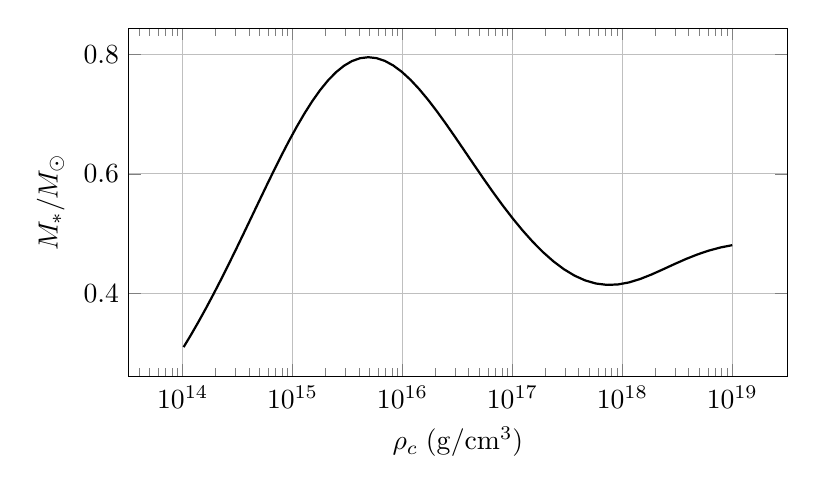
\begin{tikzpicture}\begin{semilogxaxis}[width=.82\textwidth,height=6cm,xlabel={$\rho_c\;(\mathrm{g/cm^3})$},ylabel={$M_*/M_\odot$},grid=major]
\addplot[thick] coordinates {
(1.01934485e+14,0.30984210)
(1.19089924e+14,0.33052509)
(1.39162555e+14,0.35216435)
(1.62657042e+14,0.37472814)
(1.90167800e+14,0.39816855)
(2.22395649e+14,0.42241942)
(2.60167729e+14,0.44739429)
(3.04461392e+14,0.47298452)
(3.56432905e+14,0.49905765)
(4.17452025e+14,0.52545617)
(4.89143723e+14,0.55199690)
(5.73438688e+14,0.57847105)
(6.72634570e+14,0.60464520)
(7.89470461e+14,0.63026337)
(9.27217700e+14,0.65505019)
(1.08979086e+15,0.67871541)
(1.28188376e+15,0.70095970)
(1.50913657e+15,0.72148159)
(1.77834174e+15,0.73998560)
(2.09769820e+15,0.75619101)
(2.47712631e+15,0.76984120)
(2.92865868e+15,0.78071281)
(3.46692663e+15,0.78862452)
(4.10976689e+15,0.79344458)
(4.87898030e+15,0.79509686)
(5.80128238e+15,0.79356490)
(6.90949708e+15,0.78889352)
(8.24405887e+15,0.78118812)
(9.85490655e+15,0.77061147)
(1.18038752e+16,0.75737833)
(1.41677225e+16,0.74174831)
(1.70419646e+16,0.72401736)
(2.05457441e+16,0.70450858)
(2.48280179e+16,0.68356288)
(3.00754334e+16,0.66153015)
(3.65223650e+16,0.63876127)
(4.44637186e+16,0.61560151)
(5.42712857e+16,0.59238559)
(6.64146505e+16,0.56943440)
(8.14879421e+16,0.54705362)
(1.00244094e+17,0.52553413)
(1.23638754e+17,0.50515396)
(1.52886594e+17,0.48618147)
(1.89533580e+17,0.46887910)
(2.35549771e+17,0.45350672)
(2.93448543e+17,0.44032254)
(3.66439841e+17,0.42957898)
(4.58627257e+17,0.42150977)
(5.75261570e+17,0.41630418)
(7.23067041e+17,0.41406687)
(9.10661485e+17,0.41476781)
(1.14909724e+18,0.41819618)
(1.45255800e+18,0.42393989)
(1.83925670e+18,0.43140927)
(2.33259260e+18,0.43990654)
(2.96264289e+18,0.44872103)
(3.76808570e+18,0.45721951)
(4.79867985e+18,0.46490754)
(6.11846287e+18,0.47145415)
(7.80987606e+18,0.47668574)
(9.97908595e+18,0.48056128)
};\end{semilogxaxis}\end{tikzpicture}\end{center}
\begin{figure}[htbp]\centering
\begin{tikzpicture}\begin{axis}[axis equal image,width=.42\textwidth,height=5.8cm,title={全轨道},xlabel={$x/(GM)$},ylabel={$y/(GM)$},grid=major]
\addplot[thick] coordinates {
(100.0000000,0.0000000)
(99.8264107,0.0225000)
(99.6527962,0.0450000)
(99.4791563,0.0675000)
(99.3054910,0.0899999)
(99.1318002,0.1124999)
(98.9580838,0.1349998)
(98.7843417,0.1574997)
(98.6105739,0.1799995)
(98.4367801,0.2024993)
(98.2629604,0.2249990)
(98.0891147,0.2474987)
(97.9152428,0.2699983)
(97.7413447,0.2924979)
(97.5674202,0.3149973)
(97.3934693,0.3374967)
(97.2194919,0.3599960)
(97.0454878,0.3824952)
(96.8714571,0.4049942)
(96.6973995,0.4274932)
(96.5233150,0.4499920)
(96.3492035,0.4724908)
(96.1750649,0.4949894)
(96.0008992,0.5174878)
(95.8267060,0.5399861)
(95.6524855,0.5624842)
(95.4782375,0.5849822)
(95.3039619,0.6074800)
(95.1296586,0.6299777)
(94.9553275,0.6524751)
(94.7809684,0.6749724)
(94.6065814,0.6974695)
(94.4321662,0.7199663)
(94.2577228,0.7424630)
(94.0832510,0.7649594)
(93.9087509,0.7874556)
(93.7342222,0.8099515)
(93.5596648,0.8324472)
(93.3850787,0.8549427)
(93.2104637,0.8774378)
(93.0358198,0.8999327)
(92.8611468,0.9224274)
(92.6864446,0.9449217)
(92.5117130,0.9674157)
(92.3369521,0.9899095)
(92.1621617,1.0124029)
(91.9873416,1.0348960)
(91.8124917,1.0573887)
(91.6376120,1.0798811)
(91.4627023,1.1023732)
(91.2877625,1.1248649)
(91.1127925,1.1473562)
(90.9377922,1.1698471)
(90.7627614,1.1923377)
(90.5877001,1.2148278)
(90.4126081,1.2373176)
(90.2374852,1.2598069)
(90.0623315,1.2822957)
(89.8871467,1.3047842)
(89.7119308,1.3272722)
(89.5366835,1.3497597)
(89.3614049,1.3722467)
(89.1860947,1.3947333)
(89.0107529,1.4172194)
(88.8353792,1.4397049)
(88.6599737,1.4621900)
(88.4845361,1.4846745)
(88.3090664,1.5071585)
(88.1335644,1.5296419)
(87.9580299,1.5521248)
(87.7824629,1.5746071)
(87.6068632,1.5970888)
(87.4312307,1.6195699)
(87.2555653,1.6420504)
(87.0798668,1.6645302)
(86.9041350,1.6870095)
(86.7283699,1.7094881)
(86.5525713,1.7319660)
(86.3767391,1.7544433)
(86.2008732,1.7769198)
(86.0249733,1.7993957)
(85.8490394,1.8218709)
(85.6730713,1.8443453)
(85.4970690,1.8668190)
(85.3210321,1.8892919)
(85.1449606,1.9117641)
(84.9688544,1.9342355)
(84.7927133,1.9567061)
(84.6165372,1.9791759)
(84.4403259,2.0016449)
(84.2640793,2.0241130)
(84.0877971,2.0465803)
(83.9114794,2.0690467)
(83.7351258,2.0915123)
(83.5587364,2.1139769)
(83.3823108,2.1364406)
(83.2058490,2.1589034)
(83.0293509,2.1813653)
(82.8528161,2.2038262)
(82.6762447,2.2262861)
(82.4996364,2.2487450)
(82.3229911,2.2712029)
(82.1463087,2.2936598)
(81.9695889,2.3161156)
(81.7928315,2.3385704)
(81.6160366,2.3610241)
(81.4392038,2.3834767)
(81.2623330,2.4059282)
(81.0854240,2.4283786)
(80.9084768,2.4508278)
(80.7314910,2.4732759)
(80.5544666,2.4957228)
(80.3774033,2.5181684)
(80.2003011,2.5406129)
(80.0231596,2.5630561)
(79.8459789,2.5854980)
(79.6687585,2.6079387)
(79.4914985,2.6303781)
(79.3141987,2.6528161)
(79.1368587,2.6752528)
(78.9594785,2.6976882)
(78.7820579,2.7201222)
(78.6045967,2.7425547)
(78.4270948,2.7649859)
(78.2495518,2.7874156)
(78.0719677,2.8098438)
(77.8943422,2.8322705)
(77.7166753,2.8546958)
(77.5389666,2.8771195)
(77.3612159,2.8995416)
(77.1834232,2.9219622)
(77.0055882,2.9443811)
(76.8277106,2.9667985)
(76.6497904,2.9892142)
(76.4718273,3.0116282)
(76.2938211,3.0340405)
(76.1157716,3.0564511)
(75.9376786,3.0788600)
(75.7595419,3.1012671)
(75.5813613,3.1236723)
(75.4031365,3.1460758)
(75.2248675,3.1684774)
(75.0465539,3.1908772)
(74.8681956,3.2132750)
(74.6897923,3.2356709)
(74.5113438,3.2580648)
(74.3328499,3.2804568)
(74.1543105,3.3028468)
(73.9757252,3.3252347)
(73.7970938,3.3476205)
(73.6184162,3.3700042)
(73.4396921,3.3923859)
(73.2609213,3.4147653)
(73.0821035,3.4371426)
(72.9032385,3.4595176)
(72.7243261,3.4818904)
(72.5453661,3.5042609)
(72.3663581,3.5266291)
(72.1873021,3.5489950)
(72.0081977,3.5713585)
(71.8290447,3.5937195)
(71.6498429,3.6160781)
(71.4705919,3.6384343)
(71.2912917,3.6607879)
(71.1119419,3.6831390)
(70.9325422,3.7054875)
(70.7530925,3.7278334)
(70.5735924,3.7501767)
(70.3940417,3.7725172)
(70.2144402,3.7948550)
(70.0347876,3.8171901)
(69.8550836,3.8395224)
(69.6753279,3.8618518)
(69.4955204,3.8841783)
(69.3156607,3.9065020)
(69.1357486,3.9288227)
(68.9557837,3.9511403)
(68.7757659,3.9734550)
(68.5956948,3.9957666)
(68.4155702,4.0180750)
(68.2353917,4.0403803)
(68.0551591,4.0626824)
(67.8748722,4.0849812)
(67.6945305,4.1072768)
(67.5141339,4.1295690)
(67.3336820,4.1518578)
(67.1531746,4.1741432)
(66.9726113,4.1964252)
(66.7919918,4.2187036)
(66.6113159,4.2409784)
(66.4305832,4.2632497)
(66.2497935,4.2855172)
(66.0689463,4.3077811)
(65.8880415,4.3300412)
(65.7070786,4.3522975)
(65.5260574,4.3745499)
(65.3449776,4.3967984)
(65.1638388,4.4190429)
(64.9826407,4.4412835)
(64.8013829,4.4635199)
(64.6200652,4.4857522)
(64.4386872,4.5079803)
(64.2572485,4.5302042)
(64.0757489,4.5524238)
(63.8941879,4.5746390)
(63.7125653,4.5968498)
(63.5308806,4.6190562)
(63.3491336,4.6412580)
(63.1673239,4.6634552)
(62.9854510,4.6856477)
(62.8035147,4.7078355)
(62.6215146,4.7300186)
(62.4394504,4.7521968)
(62.2573215,4.7743701)
(62.0751277,4.7965384)
(61.8928687,4.8187016)
(61.7105439,4.8408598)
(61.5281530,4.8630127)
(61.3456957,4.8851604)
(61.1631715,4.9073028)
(60.9805801,4.9294398)
(60.7979210,4.9515713)
(60.6151938,4.9736973)
(60.4323982,4.9958176)
(60.2495337,5.0179323)
(60.0665999,5.0400412)
(59.8835964,5.0621442)
(59.7005228,5.0842413)
(59.5173786,5.1063324)
(59.3341634,5.1284174)
(59.1508768,5.1504963)
(58.9675183,5.1725688)
(58.7840875,5.1946351)
(58.6005840,5.2166949)
(58.4170072,5.2387482)
(58.2333568,5.2607949)
(58.0496322,5.2828348)
(57.8658331,5.3048680)
(57.6819589,5.3268944)
(57.4980092,5.3489137)
(57.3139835,5.3709260)
(57.1298813,5.3929311)
(56.9457021,5.4149289)
(56.7614454,5.4369194)
(56.5771108,5.4589024)
(56.3926977,5.4808778)
(56.2082056,5.5028456)
(56.0236340,5.5248055)
(55.8389824,5.5467576)
(55.6542503,5.5687017)
(55.4694371,5.5906377)
(55.2845423,5.6125654)
(55.0995654,5.6344848)
(54.9145058,5.6563958)
(54.7293630,5.6782982)
(54.5441364,5.7001918)
(54.3588255,5.7220767)
(54.1734296,5.7439527)
(53.9879483,5.7658195)
(53.8023809,5.7876772)
(53.6167269,5.8095256)
(53.4309856,5.8313645)
(53.2451564,5.8531938)
(53.0592389,5.8750134)
(52.8732322,5.8968231)
(52.6871360,5.9186229)
(52.5009494,5.9404124)
(52.3146719,5.9621917)
(52.1283028,5.9839606)
(51.9418415,6.0057189)
(51.7552874,6.0274664)
(51.5686398,6.0492031)
(51.3818980,6.0709287)
(51.1950613,6.0926431)
(51.0081291,6.1143462)
(50.8211007,6.1360377)
(50.6339754,6.1577175)
(50.4467525,6.1793854)
(50.2594312,6.2010413)
(50.0720109,6.2226849)
(49.8844908,6.2443162)
(49.6968702,6.2659349)
(49.5091484,6.2875408)
(49.3213246,6.3091338)
(49.1333980,6.3307136)
(48.9453678,6.3522800)
(48.7572334,6.3738330)
(48.5689938,6.3953722)
(48.3806484,6.4168974)
(48.1921962,6.4384085)
(48.0036366,6.4599053)
(47.8149685,6.4813874)
(47.6261913,6.5028548)
(47.4373041,6.5243071)
(47.2483060,6.5457442)
(47.0591962,6.5671658)
(46.8699737,6.5885717)
(46.6806377,6.6099616)
(46.4911874,6.6313354)
(46.3016217,6.6526926)
(46.1119397,6.6740332)
(45.9221406,6.6953568)
(45.7322234,6.7166632)
(45.5421872,6.7379522)
(45.3520309,6.7592233)
(45.1617536,6.7804764)
(44.9713543,6.8017112)
(44.7808320,6.8229274)
(44.5901857,6.8441248)
(44.3994143,6.8653029)
(44.2085169,6.8864615)
(44.0174923,6.9076003)
(43.8263395,6.9287190)
(43.6350574,6.9498172)
(43.4436449,6.9708947)
(43.2521009,6.9919511)
(43.0604242,7.0129860)
(42.8686138,7.0339992)
(42.6766685,7.0549902)
(42.4845870,7.0759587)
(42.2923683,7.0969043)
(42.1000110,7.1178267)
(41.9075141,7.1387255)
(41.7148761,7.1596003)
(41.5220960,7.1804506)
(41.3291724,7.2012762)
(41.1361040,7.2220765)
(40.9428895,7.2428511)
(40.7495277,7.2635997)
(40.5560170,7.2843218)
(40.3623563,7.3050169)
(40.1685441,7.3256846)
(39.9745789,7.3463244)
(39.7804595,7.3669359)
(39.5861843,7.3875185)
(39.3917518,7.4080718)
(39.1971607,7.4285952)
(39.0024093,7.4490882)
(38.8074962,7.4695504)
(38.6124198,7.4899811)
(38.4171785,7.5103798)
(38.2217707,7.5307460)
(38.0261948,7.5510791)
(37.8304492,7.5713785)
(37.6345322,7.5916435)
(37.4384420,7.6118737)
(37.2421770,7.6320683)
(37.0457355,7.6522267)
(36.8491156,7.6723482)
(36.6523155,7.6924323)
(36.4553334,7.7124781)
(36.2581674,7.7324851)
(36.0608157,7.7524524)
(35.8632763,7.7723794)
(35.6655472,7.7922653)
(35.4676266,7.8121093)
(35.2695123,7.8319106)
(35.0712023,7.8516686)
(34.8726946,7.8713822)
(34.6739870,7.8910507)
(34.4750774,7.9106733)
(34.2759635,7.9302489)
(34.0766432,7.9497769)
(33.8771142,7.9692561)
(33.6773742,7.9886857)
(33.4774208,8.0080646)
(33.2772517,8.0273920)
(33.0768645,8.0466668)
(32.8762566,8.0658878)
(32.6754256,8.0850542)
(32.4743690,8.1041647)
(32.2730840,8.1232182)
(32.0715682,8.1422136)
(31.8698188,8.1611497)
(31.6678330,8.1800252)
(31.4656081,8.1988391)
(31.2631413,8.2175898)
(31.0604295,8.2362762)
(30.8574701,8.2548969)
(30.6542598,8.2734505)
(30.4507956,8.2919356)
(30.2470745,8.3103507)
(30.0430933,8.3286943)
(29.8388487,8.3469649)
(29.6343374,8.3651609)
(29.4295562,8.3832807)
(29.2245015,8.4013226)
(29.0191698,8.4192849)
(28.8135577,8.4371659)
(28.6076615,8.4549636)
(28.4014775,8.4726762)
(28.1950019,8.4903019)
(27.9882308,8.5078386)
(27.7811603,8.5252843)
(27.5737865,8.5426369)
(27.3661052,8.5598942)
(27.1581123,8.5770541)
(26.9498034,8.5941141)
(26.7411742,8.6110720)
(26.5322204,8.6279254)
(26.3229372,8.6446717)
(26.1133201,8.6613083)
(25.9033644,8.6778326)
(25.6930651,8.6942417)
(25.4824174,8.7105330)
(25.2714162,8.7267035)
(25.0600563,8.7427500)
(24.8483324,8.7586696)
(24.6362391,8.7744589)
(24.4237708,8.7901147)
(24.2109220,8.8056336)
(23.9976867,8.8210118)
(23.7840591,8.8362459)
(23.5700331,8.8513320)
(23.3556025,8.8662661)
(23.1407610,8.8810441)
(22.9255019,8.8956620)
(22.7098187,8.9101152)
(22.4937045,8.9243994)
(22.2771524,8.9385097)
(22.0601550,8.9524415)
(21.8427051,8.9661896)
(21.6247952,8.9797488)
(21.4064175,8.9931138)
(21.1875640,9.0062789)
(20.9682267,9.0192383)
(20.7483972,9.0319859)
(20.5280669,9.0445156)
(20.3072271,9.0568208)
(20.0858687,9.0688947)
(19.8639824,9.0807302)
(19.6415589,9.0923201)
(19.4185882,9.1036567)
(19.1950603,9.1147321)
(18.9709650,9.1255380)
(18.7462916,9.1360658)
(18.5210293,9.1463066)
(18.2951668,9.1562509)
(18.0686925,9.1658891)
(17.8415948,9.1752110)
(17.6138613,9.1842059)
(17.3854795,9.1928628)
(17.1564365,9.2011700)
(16.9267190,9.2091154)
(16.6963132,9.2166863)
(16.4652052,9.2238696)
(16.2333804,9.2306512)
(16.0008238,9.2370168)
(15.7675199,9.2429509)
(15.5334530,9.2484376)
(15.2986065,9.2534602)
(15.0629638,9.2580011)
(14.8265072,9.2620417)
(14.5892188,9.2655627)
(14.3510802,9.2685437)
(14.1120723,9.2709631)
(13.8721752,9.2727983)
(13.6313687,9.2740256)
(13.3896318,9.2746197)
(13.1469428,9.2745543)
(12.9032793,9.2738015)
(12.6586184,9.2723316)
(12.4129362,9.2701135)
(12.1662081,9.2671142)
(11.9184088,9.2632989)
(11.6695122,9.2586306)
(11.4194913,9.2530701)
(11.1683184,9.2465760)
(10.9159647,9.2391041)
(10.6624007,9.2306077)
(10.4075961,9.2210370)
(10.1515195,9.2103392)
(9.8941387,9.1984579)
(9.6354207,9.1853330)
(9.3753315,9.1709008)
(9.1138361,9.1550927)
(8.8508991,9.1378361)
(8.5970892,9.1198346)
(8.5864837,9.1190529)
(8.3312198,9.0995075)
(8.3205530,9.0986598)
(8.0637985,9.0774851)
(8.0530688,9.0765676)
(7.8055783,9.0546600)
(7.7839927,9.0526806)
(7.5350033,9.0290315)
(7.5132858,9.0268964)
(7.2627613,9.0014049)
(7.2409088,8.9991049)
(6.9888129,8.9716625)
(6.9668221,8.9691880)
(6.7241804,8.9410023)
(6.6909865,8.9370186)
(6.4467734,8.9067380)
(6.4133629,8.9024601)
(6.1675447,8.8699558)
(6.1339130,8.8653653)
(5.8977364,8.8321302)
(5.8525995,8.8255760)
(5.6148299,8.7899459)
(5.5693868,8.7829211)
(5.3299956,8.7447423)
(5.2842412,8.7372166)
(5.0432025,8.6963230)
(4.9971319,8.6882635)
(4.7660124,8.6466184)
(4.7080320,8.6358472)
(4.4753034,8.5912653)
(4.4169188,8.5797357)
(4.1825674,8.5320181)
(4.1237758,8.5196783)
(3.8877932,8.4686101)
(3.8285934,8.4554043)
(3.6028900,8.4035566)
(3.5313709,8.3866207)
(3.3041230,8.3311355)
(3.2321183,8.3130112)
(3.0033421,8.2536309)
(2.9308585,8.2342337)
(2.7005818,8.1706803)
(2.6276302,8.1499189)
(2.3958947,8.0818922)
(2.3224908,8.0596681)
(2.1016508,7.9907719)
(2.0155200,7.9630514)
(1.7934255,7.8892870)
(1.7068241,7.8596058)
(1.4835707,7.7806184)
(1.3965408,7.7488335)
(1.1722504,7.6642423)
(1.0848450,7.6302004)
(0.8596700,7.5395978)
(0.7719549,7.5031350)
(0.5460836,7.4060860)
(0.4581399,7.3670279)
(0.2318020,7.2630700)
(0.1437282,7.2212314)
(-0.0827979,7.1098753)
(-0.1708834,7.0650609)
(-0.3972639,6.9457918)
(-0.4852192,6.8977968)
(-0.7110565,6.7700772)
(-0.7987135,6.7186885)
(-1.0235375,6.5819615)
(-1.1106980,6.5269595)
(-1.3215903,6.3889699)
(-1.4203890,6.3218154)
(-1.6292088,6.1742457)
(-1.7268738,6.1024547)
(-1.9208604,5.9542351)
(-2.0290970,5.8680824)
(-2.2078884,5.7199310)
(-2.3258475,5.6179273)
(-2.5007045,5.4599540)
(-2.6157462,5.3512638)
(-2.7745237,5.1944738)
(-2.8972360,5.0674378)
(-3.0505559,4.9007875)
(-3.1685755,4.7658968)
(-3.3050276,4.6019500)
(-3.4278357,4.4462250)
(-3.5571832,4.2727426)
(-3.6729044,4.1081825)
(-3.7848317,3.9393807)
(-3.8926992,3.7663552)
(-3.9014964,3.7517467)
(-4.0046571,3.5741834)
(-4.1031810,3.3924836)
(-4.1111731,3.3771572)
(-4.1967818,3.2067153)
(-4.2780093,3.0329270)
(-4.2993722,2.9849598)
(-4.3746959,2.8070315)
(-4.4451216,2.6259617)
(-4.4634485,2.5760485)
(-4.5273101,2.3911477)
(-4.5857557,2.2033877)
(-4.6007258,2.1517036)
(-4.6475379,1.9780096)
(-4.6894725,1.8022404)
(-4.7085598,1.7136207)
(-4.7428753,1.5350031)
(-4.7719163,1.3546793)
(-4.7844118,1.2639294)
(-4.8052626,1.0813632)
(-4.8204773,0.8975294)
(-4.8259297,0.8051975)
(-4.8324462,0.6198301)
(-4.8330143,0.4337005)
(-4.8310335,0.3404180)
(-4.8224797,0.1535593)
(-4.8077281,-0.0334961)
(-4.7980028,-0.1270226)
(-4.7765150,-0.2952437)
(-4.7498705,-0.4631458)
(-4.7255592,-0.5933958)
(-4.6896672,-0.7602654)
(-4.6485453,-0.9262868)
(-4.6129405,-1.0547028)
(-4.5625082,-1.2187316)
(-4.5068499,-1.3813641)
(-4.4599602,-1.5067632)
(-4.3950703,-1.6664213)
(-4.3250396,-1.8241300)
(-4.2670495,-1.9453181)
(-4.1880124,-2.0990749)
(-4.1040027,-2.2503392)
(-4.0352751,-2.3661441)
(-3.9426303,-2.5125103)
(-3.8452618,-2.6558660)
(-3.7663339,-2.7651698)
(-3.6608412,-2.9027393)
(-3.5509492,-3.0368204)
(-3.4625212,-3.1385915)
(-3.3451434,-3.2660816)
(-3.2237576,-3.3896585)
(-3.1266747,-3.4829801)
(-2.9985515,-3.5992662)
(-2.8668679,-3.7112789)
(-2.7620960,-3.7953732)
(-2.6245117,-3.8995180)
(-2.4838576,-3.9991019)
(-2.3724555,-4.0733486)
(-2.2268011,-4.1646226)
(-2.0785960,-4.2511268)
(-1.9616841,-4.3150743)
(-1.8094167,-4.3929684)
(-1.6551313,-4.4659640)
(-1.5338596,-4.5193344)
(-1.3764610,-4.5835623)
(-1.2175763,-4.6428426)
(-1.0930925,-4.6855292)
(-0.9140706,-4.7413284)
(-0.7338772,-4.7910550)
(-0.6434185,-4.8136526)
(-0.4619282,-4.8543466)
(-0.2798709,-4.8890885)
(-0.1887016,-4.9042486)
(-0.0062217,-4.9301960)
(0.1762662,-4.9503857)
(0.2674475,-4.9583511)
(0.4495586,-4.9700870)
(0.6311729,-4.9763217)
(0.7217354,-4.9774125)
(0.9022601,-4.9756173)
(1.0818434,-4.9686268)
(1.1712316,-4.9632246)
(1.3668230,-4.9469697)
(1.5607976,-4.9248594)
(1.6133956,-4.9178382)
(1.8050587,-4.8885546)
(1.9947247,-4.8538590)
(2.0460860,-4.8434836)
(2.2330046,-4.8021902)
(2.4176208,-4.7559429)
(2.4675561,-4.7424969)
(2.6654602,-4.6852615)
(2.8603362,-4.6227003)
(2.8764358,-4.6172547)
(3.0679139,-4.5492177)
(3.2561653,-4.4763938)
(3.2717049,-4.4701170)
(3.4716207,-4.3857186)
(3.6526596,-4.3033813)
(3.8449479,-4.2096684)
(4.0188751,-4.1192466)
(4.2174403,-4.0093099)
(4.3701671,-3.9197865)
(4.5603716,-3.8021206)
(4.7065536,-3.7069318)
(4.9013014,-3.5735356)
(5.0282182,-3.4824602)
(5.2142771,-3.3428817)
(5.3354764,-3.2479920)
(5.5247507,-3.0933689)
(5.6287460,-3.0049918)
(5.8204282,-2.8355540)
(5.9085200,-2.7547724)
(6.0913346,-2.5811017)
(6.1753444,-2.4985028)
(6.3597642,-2.3108283)
(6.4297990,-2.2372176)
(6.6056825,-2.0465022)
(6.6724821,-1.9718270)
(6.8402640,-1.7786550)
(6.9039974,-1.7031276)
(7.0641104,-1.5080088)
(7.1249446,-1.4318138)
(7.2778135,-1.2351905)
(7.3359116,-1.1584879)
(7.4819493,-0.9607425)
(7.5374690,-0.8836703)
(7.6770731,-0.6851320)
(7.7301658,-0.6078088)
(7.8637167,-0.4087600)
(7.9145269,-0.3312874)
(8.0423867,-0.1319695)
(8.0910514,-0.0544340)
(8.2135629,0.1449477)
(8.2602117,0.2224725)
(8.3841235,0.4328101)
(8.4224534,0.4991958)
(8.5413886,0.7092591)
(8.5781954,0.7755366)
(8.6924552,0.9851960)
(8.7278309,1.0513279)
(8.8376971,1.2604750)
(8.8717278,1.3264301)
(8.9774642,1.5349751)
(9.0102304,1.6007278)
(9.1173651,1.8195223)
(9.1436599,1.8741260)
(9.2469531,2.0921446)
(9.2723162,2.1465475)
(9.3719930,2.3637393)
(9.3964789,2.4179302)
(9.4927494,2.6342550)
(9.5164086,2.6882250)
(9.6140566,2.9144037)
(9.6323483,2.9573938)
(9.7268203,3.1826043)
(9.7445244,3.2254081)
(9.8359984,3.4496327)
(9.8531477,3.4922474)
(9.9417900,3.7154743)
(9.9584149,3.7578981)
(10.0484199,3.9906812)
(10.0605095,4.0223524)
(10.1478644,4.2540801)
(10.1596024,4.2856073)
(10.2444482,4.5162804)
(10.2558533,4.5476640)
(10.3420223,4.7877019)
(10.3494112,4.8085272)
(10.4332259,5.0474736)
(10.4404153,5.0682044)
(10.5219957,5.3060685)
(10.5289958,5.3267056)
(10.6118661,5.5737714)
(10.6152745,5.5840427)
(10.6960422,5.8300037)
(10.6993651,5.8402292)
(10.7781329,6.0850998)
(10.7813746,6.0952802)
(10.8614028,6.3492114)
(10.9395437,6.6020396)
(11.0158852,6.8537823)
(11.0905101,7.1044572)
(11.1634961,7.3540825)
(11.2349164,7.6026766)
(11.3048398,7.8502580)
(11.3733312,8.0968452)
(11.4404518,8.3424567)
(11.5062592,8.5871108)
(11.5708079,8.8308257)
(11.6341494,9.0736195)
(11.6963324,9.3155098)
(11.7574029,9.5565142)
(11.8174044,9.7966499)
(11.8763784,10.0359339)
(11.9343639,10.2743827)
(11.9913982,10.5120127)
(12.0475164,10.7488397)
(12.1027521,10.9848795)
(12.1571371,11.2201472)
(12.2107018,11.4546579)
(12.2634749,11.6884261)
(12.3154839,11.9214662)
(12.3667550,12.1537920)
(12.4173131,12.3854171)
(12.4671820,12.6163549)
(12.5163844,12.8466182)
(12.5649420,13.0762198)
(12.6128755,13.3051720)
(12.6602047,13.5334868)
(12.7069486,13.7611759)
(12.7531253,13.9882508)
(12.7987522,14.2147227)
(12.8438459,14.4406025)
(12.8884223,14.6659007)
(12.9324968,14.8906278)
(12.9760840,15.1147938)
(13.0191979,15.3384086)
(13.0618521,15.5614819)
(13.1040596,15.7840229)
(13.1458328,16.0060409)
(13.1871838,16.2275448)
(13.2281240,16.4485433)
(13.2686646,16.6690449)
(13.3088162,16.8890579)
(13.3485892,17.1085904)
(13.3879934,17.3276503)
(13.4270385,17.5462453)
(13.4657335,17.7643830)
(13.5040874,17.9820707)
(13.5421088,18.1993156)
(13.5798059,18.4161247)
(13.6171868,18.6325049)
(13.6542590,18.8484629)
(13.6910301,19.0640053)
(13.7275073,19.2791383)
(13.7636975,19.4938684)
(13.7996074,19.7082015)
(13.8352436,19.9221437)
(13.8706124,20.1357008)
(13.9057198,20.3488785)
(13.9405718,20.5616825)
(13.9751741,20.7741181)
(14.0095321,20.9861907)
(14.0436514,21.1979056)
(14.0775370,21.4092679)
(14.1111940,21.6202825)
(14.1446274,21.8309544)
(14.1778418,22.0412885)
(14.2108419,22.2512893)
(14.2436320,22.4609615)
(14.2762167,22.6703096)
(14.3086000,22.8793380)
(14.3407861,23.0880510)
(14.3727789,23.2964529)
(14.4045824,23.5045478)
(14.4362002,23.7123398)
(14.4676360,23.9198329)
(14.4988933,24.1270310)
(14.5299757,24.3339378)
(14.5608864,24.5405573)
(14.5916288,24.7468930)
(14.6222059,24.9529485)
(14.6526210,25.1587274)
(14.6828770,25.3642333)
(14.7129769,25.5694694)
(14.7429235,25.7744391)
(14.7727196,25.9791457)
(14.8023680,26.1835924)
(14.8318711,26.3877825)
(14.8612318,26.5917189)
(14.8904524,26.7954047)
(14.9195354,26.9988430)
(14.9484832,27.2020366)
(14.9772982,27.4049885)
(15.0059826,27.6077014)
(15.0345386,27.8101782)
(15.0629684,28.0124215)
(15.0912742,28.2144342)
(15.1194579,28.4162187)
(15.1475217,28.6177777)
(15.1754674,28.8191137)
(15.2032971,29.0202293)
(15.2310125,29.2211268)
(15.2586155,29.4218088)
(15.2861080,29.6222776)
(15.3134917,29.8225354)
(15.3407682,30.0225848)
(15.3679394,30.2224277)
(15.3950067,30.4220666)
(15.4219719,30.6215036)
(15.4488364,30.8207408)
(15.4756019,31.0197804)
(15.5022698,31.2186244)
(15.5288416,31.4172749)
(15.5553188,31.6157338)
(15.5817027,31.8140033)
(15.6079948,32.0120851)
(15.6341963,32.2099814)
(15.6603086,32.4076938)
(15.6863330,32.6052244)
(15.7122708,32.8025749)
(15.7381232,32.9997471)
(15.7638914,33.1967428)
(15.7895767,33.3935638)
(15.8151801,33.5902117)
(15.8407029,33.7866884)
(15.8661461,33.9829954)
(15.8915109,34.1791344)
(15.9167984,34.3751070)
(15.9420095,34.5709148)
(15.9671454,34.7665594)
(15.9922070,34.9620423)
(16.0171953,35.1573651)
(16.0421114,35.3525293)
(16.0669562,35.5475363)
(16.0917307,35.7423877)
(16.1164357,35.9370848)
(16.1410721,36.1316291)
(16.1656409,36.3260220)
(16.1901430,36.5202649)
(16.2145791,36.7143591)
(16.2389502,36.9083060)
(16.2632570,37.1021069)
(16.2875004,37.2957630)
(16.3116812,37.4892758)
(16.3358002,37.6826465)
(16.3598581,37.8758762)
(16.3838556,38.0689664)
(16.4077936,38.2619181)
(16.4316727,38.4547326)
(16.4554938,38.6474111)
(16.4792574,38.8399547)
(16.5029642,39.0323646)
(16.5266151,39.2246420)
(16.5502105,39.4167879)
(16.5737512,39.6088035)
(16.5972379,39.8006899)
(16.6206711,39.9924481)
(16.6440515,40.1840793)
(16.6673798,40.3755845)
(16.6906564,40.5669647)
(16.7138820,40.7582209)
(16.7370573,40.9493543)
(16.7601827,41.1403657)
(16.7832588,41.3312561)
(16.8062862,41.5220267)
(16.8292654,41.7126782)
(16.8521971,41.9032117)
(16.8750816,42.0936281)
(16.8979196,42.2839283)
(16.9207115,42.4741133)
(16.9434579,42.6641840)
(16.9661592,42.8541412)
(16.9888159,43.0439859)
(17.0114286,43.2337188)
(17.0339977,43.4233410)
(17.0565236,43.6128533)
(17.0790069,43.8022564)
(17.1014480,43.9915512)
(17.1238473,44.1807386)
(17.1462052,44.3698194)
(17.1685223,44.5587943)
(17.1907989,44.7476642)
(17.2130354,44.9364299)
(17.2352323,45.1250920)
(17.2573900,45.3136515)
(17.2795089,45.5021091)
(17.3015893,45.6904655)
(17.3236317,45.8787214)
(17.3456364,46.0668776)
(17.3676039,46.2549348)
(17.3895345,46.4428938)
(17.4114286,46.6307552)
(17.4332865,46.8185198)
(17.4551086,47.0061882)
(17.4768952,47.1937612)
(17.4986467,47.3812394)
(17.5203635,47.5686234)
(17.5420459,47.7559140)
(17.5636942,47.9431118)
(17.5853087,48.1302175)
(17.6068898,48.3172317)
(17.6284378,48.5041550)
(17.6499530,48.6909881)
(17.6714357,48.8777315)
(17.6928862,49.0643860)
(17.7143049,49.2509521)
(17.7356919,49.4374304)
(17.7570478,49.6238216)
(17.7783726,49.8101261)
(17.7996667,49.9963447)
(17.8209304,50.1824778)
(17.8421640,50.3685260)
(17.8633677,50.5544900)
(17.8845419,50.7403703)
(17.9056867,50.9261674)
(17.9268025,51.1118818)
(17.9478895,51.2975142)
(17.9689479,51.4830650)
(17.9899781,51.6685349)
(18.0109803,51.8539242)
(18.0319547,52.0392336)
(18.0529015,52.2244636)
(18.0738211,52.4096147)
(18.0947137,52.5946873)
(18.1155794,52.7796820)
(18.1364186,52.9645993)
(18.1572314,53.1494396)
(18.1780181,53.3342036)
(18.1987789,53.5188915)
(18.2195141,53.7035040)
(18.2402238,53.8880415)
(18.2609082,54.0725044)
(18.2815677,54.2568933)
(18.3022024,54.4412086)
(18.3228124,54.6254507)
(18.3433981,54.8096201)
(18.3639596,54.9937172)
(18.3844971,55.1777425)
(18.4050108,55.3616964)
(18.4255010,55.5455794)
(18.4459677,55.7293919)
(18.4664113,55.9131343)
(18.4868318,56.0968071)
(18.5072295,56.2804105)
(18.5276046,56.4639452)
(18.5479573,56.6474114)
(18.5682876,56.8308096)
(18.5885959,57.0141402)
(18.6088823,57.1974036)
(18.6291469,57.3806002)
(18.6493900,57.5637304)
(18.6696116,57.7467945)
(18.6898121,57.9297930)
(18.7099915,58.1127262)
(18.7301499,58.2955945)
(18.7502877,58.4783983)
(18.7704049,58.6611379)
(18.7905017,58.8438138)
(18.8105782,59.0264263)
(18.8306347,59.2089757)
(18.8506712,59.3914625)
(18.8706880,59.5738869)
(18.8906851,59.7562493)
(18.9106627,59.9385501)
(18.9306210,60.1207896)
(18.9505600,60.3029682)
(18.9704801,60.4850862)
(18.9903812,60.6671439)
(19.0102636,60.8491417)
(19.0301274,61.0310799)
(19.0499727,61.2129589)
(19.0697997,61.3947789)
(19.0896084,61.5765402)
(19.1093991,61.7582433)
(19.1291718,61.9398884)
(19.1489267,62.1214759)
(19.1686640,62.3030060)
(19.1883837,62.4844790)
(19.2080859,62.6658953)
(19.2277709,62.8472552)
(19.2474387,63.0285590)
(19.2670895,63.2098070)
(19.2867233,63.3909994)
(19.3063404,63.5721366)
(19.3259407,63.7532189)
(19.3455245,63.9342465)
(19.3650918,64.1152197)
(19.3846428,64.2961389)
(19.4041776,64.4770043)
(19.4236963,64.6578162)
(19.4431990,64.8385748)
(19.4626858,65.0192805)
(19.4821568,65.1999335)
(19.5016122,65.3805341)
(19.5210520,65.5610826)
(19.5404764,65.7415792)
(19.5598855,65.9220241)
(19.5792793,66.1024178)
(19.5986580,66.2827604)
(19.6180216,66.4630521)
(19.6373704,66.6432933)
(19.6567043,66.8234842)
(19.6760235,67.0036250)
(19.6953280,67.1837161)
(19.7146181,67.3637575)
(19.7338937,67.5437497)
(19.7531549,67.7236928)
(19.7724020,67.9035872)
(19.7916349,68.0834329)
(19.8108537,68.2632303)
(19.8300586,68.4429796)
(19.8492496,68.6226811)
(19.8684269,68.8023349)
(19.8875904,68.9819413)
(19.9067404,69.1615006)
(19.9258769,69.3410130)
(19.9449999,69.5204786)
(19.9641096,69.6998978)
(19.9832061,69.8792708)
(20.0022894,70.0585977)
(20.0213596,70.2378788)
(20.0404168,70.4171143)
(20.0594611,70.5963045)
(20.0784926,70.7754495)
(20.0975113,70.9545495)
(20.1165174,71.1336049)
(20.1355109,71.3126157)
(20.1544919,71.4915822)
(20.1734604,71.6705047)
(20.1924166,71.8493832)
(20.2113605,72.0282181)
(20.2302922,72.2070095)
(20.2492118,72.3857576)
(20.2681193,72.5644627)
(20.2870149,72.7431249)
(20.3058986,72.9217444)
(20.3247704,73.1003214)
(20.3436305,73.2788561)
(20.3624789,73.4573488)
(20.3813157,73.6357996)
(20.4001409,73.8142086)
(20.4189547,73.9925762)
(20.4377570,74.1709024)
(20.4565481,74.3491875)
(20.4753278,74.5274316)
(20.4940964,74.7056350)
(20.5128538,74.8837978)
(20.5316002,75.0619201)
(20.5503355,75.2400023)
(20.5690600,75.4180444)
(20.5877735,75.5960467)
(20.6064762,75.7740093)
(20.6251682,75.9519324)
(20.6438496,76.1298161)
(20.6625203,76.3076607)
(20.6811804,76.4854663)
(20.6998301,76.6632330)
(20.7184693,76.8409612)
(20.7370981,77.0186508)
(20.7557166,77.1963022)
(20.7743249,77.3739154)
(20.7929230,77.5514907)
(20.8115109,77.7290281)
(20.8300888,77.9065279)
(20.8486566,78.0839902)
(20.8672145,78.2614151)
(20.8857624,78.4388029)
(20.9043006,78.6161537)
(20.9228289,78.7934677)
(20.9413474,78.9707450)
(20.9598563,79.1479857)
(20.9783556,79.3251901)
(20.9968452,79.5023582)
(21.0153254,79.6794903)
(21.0337960,79.8565865)
(21.0522573,80.0336468)
(21.0707092,80.2106716)
(21.0891517,80.3876609)
(21.1075850,80.5646149)
(21.1260091,80.7415337)
(21.1444240,80.9184175)
(21.1628298,81.0952664)
(21.1812266,81.2720806)
(21.1996143,81.4488602)
(21.2179931,81.6256053)
(21.2363629,81.8023161)
(21.2547239,81.9789928)
(21.2730760,82.1556354)
(21.2914194,82.3322442)
(21.3097540,82.5088192)
(21.3280800,82.6853606)
(21.3463973,82.8618685)
(21.3647061,83.0383430)
(21.3830063,83.2147844)
(21.4012980,83.3911927)
(21.4195812,83.5675681)
(21.4378560,83.7439106)
(21.4561225,83.9202205)
(21.4743807,84.0964978)
(21.4926305,84.2727427)
(21.5108722,84.4489554)
(21.5291056,84.6251359)
(21.5473309,84.8012843)
(21.5655481,84.9774009)
(21.5837573,85.1534856)
(21.6019584,85.3295388)
(21.6201515,85.5055604)
(21.6383367,85.6815506)
(21.6565140,85.8575095)
(21.6746834,86.0334372)
(21.6928450,86.2093340)
(21.7109989,86.3851998)
(21.7291450,86.5610348)
(21.7472834,86.7368391)
(21.7654141,86.9126129)
(21.7835372,87.0883563)
(21.8016527,87.2640693)
(21.8197607,87.4397521)
(21.8378612,87.6154048)
(21.8559542,87.7910276)
(21.8740397,87.9666205)
(21.8921179,88.1421837)
(21.9101887,88.3177172)
(21.9282522,88.4932212)
(21.9463084,88.6686958)
(21.9643574,88.8441411)
(21.9823991,89.0195572)
(22.0004336,89.1949442)
(22.0184611,89.3703023)
(22.0364814,89.5456315)
(22.0544946,89.7209319)
(22.0725008,89.8962038)
(22.0904999,90.0714470)
(22.1084921,90.2466619)
(22.1264774,90.4218484)
(22.1444558,90.5970067)
(22.1624272,90.7721369)
(22.1803919,90.9472391)
(22.1983497,91.1223134)
(22.2163008,91.2973598)
(22.2342451,91.4723786)
(22.2521827,91.6473698)
(22.2701137,91.8223334)
(22.2880380,91.9972697)
(22.3059557,92.1721787)
(22.3238668,92.3470604)
(22.3417713,92.5219151)
(22.3596693,92.6967427)
(22.3775609,92.8715435)
(22.3954459,93.0463174)
(22.4133246,93.2210647)
(22.4311968,93.3957853)
(22.4490627,93.5704794)
(22.4669223,93.7451470)
(22.4847755,93.9197883)
(22.5026224,94.0944034)
(22.5204631,94.2689924)
(22.5382976,94.4435553)
(22.5561258,94.6180922)
(22.5739480,94.7926033)
(22.5917639,94.9670886)
(22.6095738,95.1415482)
(22.6273776,95.3159822)
(22.6451753,95.4903907)
(22.6629670,95.6647737)
(22.6807527,95.8391315)
(22.6985324,96.0134640)
(22.7163061,96.1877714)
(22.7340740,96.3620537)
(22.7518360,96.5363110)
(22.7695921,96.7105435)
(22.7873423,96.8847511)
(22.8050868,97.0589340)
(22.8228254,97.2330923)
(22.8405583,97.4072260)
(22.8582855,97.5813353)
(22.8760069,97.7554202)
(22.8937227,97.9294808)
(22.9114328,98.1035172)
(22.9291372,98.2775294)
(22.9468361,98.4515176)
(22.9645293,98.6254819)
(22.9822170,98.7994222)
(22.9998992,98.9733388)
(23.0175759,99.1472316)
(23.0352470,99.3211008)
(23.0529127,99.4949464)
(23.0705730,99.6687685)
(23.0882278,99.8425672)
(23.1058773,100.0163426)
(23.1235214,100.1900948)
(23.1411601,100.3638238)
(23.1587935,100.5375296)
(23.1764216,100.7112125)
(23.1940444,100.8848724)
(23.2116620,101.0585095)
(23.2292743,101.2321237)
(23.2468814,101.4057153)
(23.2644833,101.5792842)
(23.2820801,101.7528305)
(23.2996717,101.9263544)
(23.3172582,102.0998558)
(23.3348396,102.2733349)
(23.3524159,102.4467917)
(23.3699871,102.6202263)
(23.3875533,102.7936388)
(23.4051145,102.9670293)
(23.4226707,103.1403977)
(23.4402219,103.3137443)
(23.4577682,103.4870690)
(23.4753095,103.6603719)
(23.4928459,103.8336531)
(23.5103774,104.0069127)
(23.5279041,104.1801508)
(23.5454258,104.3533673)
(23.5629428,104.5265624)
(23.5804549,104.6997362)
(23.5979623,104.8728887)
(23.6154649,105.0460199)
(23.6329627,105.2191301)
(23.6504557,105.3922191)
(23.6679441,105.5652871)
(23.6854278,105.7383342)
(23.7029068,105.9113603)
(23.7203811,106.0843657)
(23.7378508,106.2573503)
(23.7553159,106.4303142)
(23.7727763,106.6032575)
(23.7902322,106.7761803)
(23.8076835,106.9490825)
(23.8251303,107.1219643)
(23.8425725,107.2948258)
(23.8600102,107.4676669)
(23.8774435,107.6404878)
(23.8948722,107.8132885)
(23.9122965,107.9860691)
(23.9297164,108.1588297)
(23.9471318,108.3315703)
(23.9645428,108.5042909)
(23.9819495,108.6769917)
(23.9993517,108.8496726)
(24.0167497,109.0223339)
(24.0341432,109.1949754)
(24.0515325,109.3675973)
(24.0689174,109.5401996)
(24.0862981,109.7127825)
(24.1036745,109.8853459)
(24.1210467,110.0578899)
(24.1384146,110.2304145)
(24.1557783,110.4029199)
(24.1731378,110.5754061)
(24.1904931,110.7478731)
(24.2078442,110.9203211)
(24.2251912,111.0927500)
(24.2425340,111.2651599)
(24.2598727,111.4375509)
(24.2772073,111.6099230)
(24.2945378,111.7822763)
(24.3118643,111.9546109)
(24.3291866,112.1269267)
(24.3465050,112.2992239)
(24.3638193,112.4715026)
(24.3811295,112.6437627)
(24.3984358,112.8160043)
(24.4157381,112.9882274)
(24.4330365,113.1604323)
(24.4503308,113.3326188)
(24.4676213,113.5047870)
(24.4849078,113.6769370)
(24.5021904,113.8490689)
(24.5194691,114.0211827)
(24.5367439,114.1932784)
(24.5540149,114.3653561)
(24.5712820,114.5374159)
(24.5885452,114.7094578)
(24.6058047,114.8814818)
(24.6230603,115.0534881)
(24.6403121,115.2254766)
(24.6575602,115.3974474)
(24.6748045,115.5694006)
(24.6920450,115.7413363)
(24.7092818,115.9132543)
(24.7265149,116.0851549)
(24.7437442,116.2570381)
(24.7609699,116.4289039)
(24.7781918,116.6007524)
(24.7954101,116.7725835)
(24.8126248,116.9443975)
(24.8298357,117.1161942)
(24.8470431,117.2879739)
(24.8642468,117.4597364)
(24.8814470,117.6314819)
(24.8986435,117.8032104)
(24.9158365,117.9749220)
(24.9330258,118.1466166)
(24.9502117,118.3182945)
(24.9673940,118.4899555)
(24.9845727,118.6615998)
(25.0017480,118.8332273)
(25.0189197,119.0048382)
(25.0360879,119.1764325)
(25.0532527,119.3480103)
(25.0704140,119.5195715)
(25.0875718,119.6911162)
(25.0875718,119.6911162)
};\addplot[domain=0:360,samples=100,dashed] ({2*cos(x)},{2*sin(x)});\end{axis}\end{tikzpicture}
\begin{tikzpicture}\begin{axis}[axis equal image,width=.42\textwidth,height=5.8cm,title={近黑洞区域},xlabel={$x/(GM)$},ylabel={$y/(GM)$},grid=major,xmin=-12,xmax=12,ymin=-12,ymax=12]
\addplot[thick] coordinates {
(100.0000000,0.0000000)
(99.8264107,0.0225000)
(99.6527962,0.0450000)
(99.4791563,0.0675000)
(99.3054910,0.0899999)
(99.1318002,0.1124999)
(98.9580838,0.1349998)
(98.7843417,0.1574997)
(98.6105739,0.1799995)
(98.4367801,0.2024993)
(98.2629604,0.2249990)
(98.0891147,0.2474987)
(97.9152428,0.2699983)
(97.7413447,0.2924979)
(97.5674202,0.3149973)
(97.3934693,0.3374967)
(97.2194919,0.3599960)
(97.0454878,0.3824952)
(96.8714571,0.4049942)
(96.6973995,0.4274932)
(96.5233150,0.4499920)
(96.3492035,0.4724908)
(96.1750649,0.4949894)
(96.0008992,0.5174878)
(95.8267060,0.5399861)
(95.6524855,0.5624842)
(95.4782375,0.5849822)
(95.3039619,0.6074800)
(95.1296586,0.6299777)
(94.9553275,0.6524751)
(94.7809684,0.6749724)
(94.6065814,0.6974695)
(94.4321662,0.7199663)
(94.2577228,0.7424630)
(94.0832510,0.7649594)
(93.9087509,0.7874556)
(93.7342222,0.8099515)
(93.5596648,0.8324472)
(93.3850787,0.8549427)
(93.2104637,0.8774378)
(93.0358198,0.8999327)
(92.8611468,0.9224274)
(92.6864446,0.9449217)
(92.5117130,0.9674157)
(92.3369521,0.9899095)
(92.1621617,1.0124029)
(91.9873416,1.0348960)
(91.8124917,1.0573887)
(91.6376120,1.0798811)
(91.4627023,1.1023732)
(91.2877625,1.1248649)
(91.1127925,1.1473562)
(90.9377922,1.1698471)
(90.7627614,1.1923377)
(90.5877001,1.2148278)
(90.4126081,1.2373176)
(90.2374852,1.2598069)
(90.0623315,1.2822957)
(89.8871467,1.3047842)
(89.7119308,1.3272722)
(89.5366835,1.3497597)
(89.3614049,1.3722467)
(89.1860947,1.3947333)
(89.0107529,1.4172194)
(88.8353792,1.4397049)
(88.6599737,1.4621900)
(88.4845361,1.4846745)
(88.3090664,1.5071585)
(88.1335644,1.5296419)
(87.9580299,1.5521248)
(87.7824629,1.5746071)
(87.6068632,1.5970888)
(87.4312307,1.6195699)
(87.2555653,1.6420504)
(87.0798668,1.6645302)
(86.9041350,1.6870095)
(86.7283699,1.7094881)
(86.5525713,1.7319660)
(86.3767391,1.7544433)
(86.2008732,1.7769198)
(86.0249733,1.7993957)
(85.8490394,1.8218709)
(85.6730713,1.8443453)
(85.4970690,1.8668190)
(85.3210321,1.8892919)
(85.1449606,1.9117641)
(84.9688544,1.9342355)
(84.7927133,1.9567061)
(84.6165372,1.9791759)
(84.4403259,2.0016449)
(84.2640793,2.0241130)
(84.0877971,2.0465803)
(83.9114794,2.0690467)
(83.7351258,2.0915123)
(83.5587364,2.1139769)
(83.3823108,2.1364406)
(83.2058490,2.1589034)
(83.0293509,2.1813653)
(82.8528161,2.2038262)
(82.6762447,2.2262861)
(82.4996364,2.2487450)
(82.3229911,2.2712029)
(82.1463087,2.2936598)
(81.9695889,2.3161156)
(81.7928315,2.3385704)
(81.6160366,2.3610241)
(81.4392038,2.3834767)
(81.2623330,2.4059282)
(81.0854240,2.4283786)
(80.9084768,2.4508278)
(80.7314910,2.4732759)
(80.5544666,2.4957228)
(80.3774033,2.5181684)
(80.2003011,2.5406129)
(80.0231596,2.5630561)
(79.8459789,2.5854980)
(79.6687585,2.6079387)
(79.4914985,2.6303781)
(79.3141987,2.6528161)
(79.1368587,2.6752528)
(78.9594785,2.6976882)
(78.7820579,2.7201222)
(78.6045967,2.7425547)
(78.4270948,2.7649859)
(78.2495518,2.7874156)
(78.0719677,2.8098438)
(77.8943422,2.8322705)
(77.7166753,2.8546958)
(77.5389666,2.8771195)
(77.3612159,2.8995416)
(77.1834232,2.9219622)
(77.0055882,2.9443811)
(76.8277106,2.9667985)
(76.6497904,2.9892142)
(76.4718273,3.0116282)
(76.2938211,3.0340405)
(76.1157716,3.0564511)
(75.9376786,3.0788600)
(75.7595419,3.1012671)
(75.5813613,3.1236723)
(75.4031365,3.1460758)
(75.2248675,3.1684774)
(75.0465539,3.1908772)
(74.8681956,3.2132750)
(74.6897923,3.2356709)
(74.5113438,3.2580648)
(74.3328499,3.2804568)
(74.1543105,3.3028468)
(73.9757252,3.3252347)
(73.7970938,3.3476205)
(73.6184162,3.3700042)
(73.4396921,3.3923859)
(73.2609213,3.4147653)
(73.0821035,3.4371426)
(72.9032385,3.4595176)
(72.7243261,3.4818904)
(72.5453661,3.5042609)
(72.3663581,3.5266291)
(72.1873021,3.5489950)
(72.0081977,3.5713585)
(71.8290447,3.5937195)
(71.6498429,3.6160781)
(71.4705919,3.6384343)
(71.2912917,3.6607879)
(71.1119419,3.6831390)
(70.9325422,3.7054875)
(70.7530925,3.7278334)
(70.5735924,3.7501767)
(70.3940417,3.7725172)
(70.2144402,3.7948550)
(70.0347876,3.8171901)
(69.8550836,3.8395224)
(69.6753279,3.8618518)
(69.4955204,3.8841783)
(69.3156607,3.9065020)
(69.1357486,3.9288227)
(68.9557837,3.9511403)
(68.7757659,3.9734550)
(68.5956948,3.9957666)
(68.4155702,4.0180750)
(68.2353917,4.0403803)
(68.0551591,4.0626824)
(67.8748722,4.0849812)
(67.6945305,4.1072768)
(67.5141339,4.1295690)
(67.3336820,4.1518578)
(67.1531746,4.1741432)
(66.9726113,4.1964252)
(66.7919918,4.2187036)
(66.6113159,4.2409784)
(66.4305832,4.2632497)
(66.2497935,4.2855172)
(66.0689463,4.3077811)
(65.8880415,4.3300412)
(65.7070786,4.3522975)
(65.5260574,4.3745499)
(65.3449776,4.3967984)
(65.1638388,4.4190429)
(64.9826407,4.4412835)
(64.8013829,4.4635199)
(64.6200652,4.4857522)
(64.4386872,4.5079803)
(64.2572485,4.5302042)
(64.0757489,4.5524238)
(63.8941879,4.5746390)
(63.7125653,4.5968498)
(63.5308806,4.6190562)
(63.3491336,4.6412580)
(63.1673239,4.6634552)
(62.9854510,4.6856477)
(62.8035147,4.7078355)
(62.6215146,4.7300186)
(62.4394504,4.7521968)
(62.2573215,4.7743701)
(62.0751277,4.7965384)
(61.8928687,4.8187016)
(61.7105439,4.8408598)
(61.5281530,4.8630127)
(61.3456957,4.8851604)
(61.1631715,4.9073028)
(60.9805801,4.9294398)
(60.7979210,4.9515713)
(60.6151938,4.9736973)
(60.4323982,4.9958176)
(60.2495337,5.0179323)
(60.0665999,5.0400412)
(59.8835964,5.0621442)
(59.7005228,5.0842413)
(59.5173786,5.1063324)
(59.3341634,5.1284174)
(59.1508768,5.1504963)
(58.9675183,5.1725688)
(58.7840875,5.1946351)
(58.6005840,5.2166949)
(58.4170072,5.2387482)
(58.2333568,5.2607949)
(58.0496322,5.2828348)
(57.8658331,5.3048680)
(57.6819589,5.3268944)
(57.4980092,5.3489137)
(57.3139835,5.3709260)
(57.1298813,5.3929311)
(56.9457021,5.4149289)
(56.7614454,5.4369194)
(56.5771108,5.4589024)
(56.3926977,5.4808778)
(56.2082056,5.5028456)
(56.0236340,5.5248055)
(55.8389824,5.5467576)
(55.6542503,5.5687017)
(55.4694371,5.5906377)
(55.2845423,5.6125654)
(55.0995654,5.6344848)
(54.9145058,5.6563958)
(54.7293630,5.6782982)
(54.5441364,5.7001918)
(54.3588255,5.7220767)
(54.1734296,5.7439527)
(53.9879483,5.7658195)
(53.8023809,5.7876772)
(53.6167269,5.8095256)
(53.4309856,5.8313645)
(53.2451564,5.8531938)
(53.0592389,5.8750134)
(52.8732322,5.8968231)
(52.6871360,5.9186229)
(52.5009494,5.9404124)
(52.3146719,5.9621917)
(52.1283028,5.9839606)
(51.9418415,6.0057189)
(51.7552874,6.0274664)
(51.5686398,6.0492031)
(51.3818980,6.0709287)
(51.1950613,6.0926431)
(51.0081291,6.1143462)
(50.8211007,6.1360377)
(50.6339754,6.1577175)
(50.4467525,6.1793854)
(50.2594312,6.2010413)
(50.0720109,6.2226849)
(49.8844908,6.2443162)
(49.6968702,6.2659349)
(49.5091484,6.2875408)
(49.3213246,6.3091338)
(49.1333980,6.3307136)
(48.9453678,6.3522800)
(48.7572334,6.3738330)
(48.5689938,6.3953722)
(48.3806484,6.4168974)
(48.1921962,6.4384085)
(48.0036366,6.4599053)
(47.8149685,6.4813874)
(47.6261913,6.5028548)
(47.4373041,6.5243071)
(47.2483060,6.5457442)
(47.0591962,6.5671658)
(46.8699737,6.5885717)
(46.6806377,6.6099616)
(46.4911874,6.6313354)
(46.3016217,6.6526926)
(46.1119397,6.6740332)
(45.9221406,6.6953568)
(45.7322234,6.7166632)
(45.5421872,6.7379522)
(45.3520309,6.7592233)
(45.1617536,6.7804764)
(44.9713543,6.8017112)
(44.7808320,6.8229274)
(44.5901857,6.8441248)
(44.3994143,6.8653029)
(44.2085169,6.8864615)
(44.0174923,6.9076003)
(43.8263395,6.9287190)
(43.6350574,6.9498172)
(43.4436449,6.9708947)
(43.2521009,6.9919511)
(43.0604242,7.0129860)
(42.8686138,7.0339992)
(42.6766685,7.0549902)
(42.4845870,7.0759587)
(42.2923683,7.0969043)
(42.1000110,7.1178267)
(41.9075141,7.1387255)
(41.7148761,7.1596003)
(41.5220960,7.1804506)
(41.3291724,7.2012762)
(41.1361040,7.2220765)
(40.9428895,7.2428511)
(40.7495277,7.2635997)
(40.5560170,7.2843218)
(40.3623563,7.3050169)
(40.1685441,7.3256846)
(39.9745789,7.3463244)
(39.7804595,7.3669359)
(39.5861843,7.3875185)
(39.3917518,7.4080718)
(39.1971607,7.4285952)
(39.0024093,7.4490882)
(38.8074962,7.4695504)
(38.6124198,7.4899811)
(38.4171785,7.5103798)
(38.2217707,7.5307460)
(38.0261948,7.5510791)
(37.8304492,7.5713785)
(37.6345322,7.5916435)
(37.4384420,7.6118737)
(37.2421770,7.6320683)
(37.0457355,7.6522267)
(36.8491156,7.6723482)
(36.6523155,7.6924323)
(36.4553334,7.7124781)
(36.2581674,7.7324851)
(36.0608157,7.7524524)
(35.8632763,7.7723794)
(35.6655472,7.7922653)
(35.4676266,7.8121093)
(35.2695123,7.8319106)
(35.0712023,7.8516686)
(34.8726946,7.8713822)
(34.6739870,7.8910507)
(34.4750774,7.9106733)
(34.2759635,7.9302489)
(34.0766432,7.9497769)
(33.8771142,7.9692561)
(33.6773742,7.9886857)
(33.4774208,8.0080646)
(33.2772517,8.0273920)
(33.0768645,8.0466668)
(32.8762566,8.0658878)
(32.6754256,8.0850542)
(32.4743690,8.1041647)
(32.2730840,8.1232182)
(32.0715682,8.1422136)
(31.8698188,8.1611497)
(31.6678330,8.1800252)
(31.4656081,8.1988391)
(31.2631413,8.2175898)
(31.0604295,8.2362762)
(30.8574701,8.2548969)
(30.6542598,8.2734505)
(30.4507956,8.2919356)
(30.2470745,8.3103507)
(30.0430933,8.3286943)
(29.8388487,8.3469649)
(29.6343374,8.3651609)
(29.4295562,8.3832807)
(29.2245015,8.4013226)
(29.0191698,8.4192849)
(28.8135577,8.4371659)
(28.6076615,8.4549636)
(28.4014775,8.4726762)
(28.1950019,8.4903019)
(27.9882308,8.5078386)
(27.7811603,8.5252843)
(27.5737865,8.5426369)
(27.3661052,8.5598942)
(27.1581123,8.5770541)
(26.9498034,8.5941141)
(26.7411742,8.6110720)
(26.5322204,8.6279254)
(26.3229372,8.6446717)
(26.1133201,8.6613083)
(25.9033644,8.6778326)
(25.6930651,8.6942417)
(25.4824174,8.7105330)
(25.2714162,8.7267035)
(25.0600563,8.7427500)
(24.8483324,8.7586696)
(24.6362391,8.7744589)
(24.4237708,8.7901147)
(24.2109220,8.8056336)
(23.9976867,8.8210118)
(23.7840591,8.8362459)
(23.5700331,8.8513320)
(23.3556025,8.8662661)
(23.1407610,8.8810441)
(22.9255019,8.8956620)
(22.7098187,8.9101152)
(22.4937045,8.9243994)
(22.2771524,8.9385097)
(22.0601550,8.9524415)
(21.8427051,8.9661896)
(21.6247952,8.9797488)
(21.4064175,8.9931138)
(21.1875640,9.0062789)
(20.9682267,9.0192383)
(20.7483972,9.0319859)
(20.5280669,9.0445156)
(20.3072271,9.0568208)
(20.0858687,9.0688947)
(19.8639824,9.0807302)
(19.6415589,9.0923201)
(19.4185882,9.1036567)
(19.1950603,9.1147321)
(18.9709650,9.1255380)
(18.7462916,9.1360658)
(18.5210293,9.1463066)
(18.2951668,9.1562509)
(18.0686925,9.1658891)
(17.8415948,9.1752110)
(17.6138613,9.1842059)
(17.3854795,9.1928628)
(17.1564365,9.2011700)
(16.9267190,9.2091154)
(16.6963132,9.2166863)
(16.4652052,9.2238696)
(16.2333804,9.2306512)
(16.0008238,9.2370168)
(15.7675199,9.2429509)
(15.5334530,9.2484376)
(15.2986065,9.2534602)
(15.0629638,9.2580011)
(14.8265072,9.2620417)
(14.5892188,9.2655627)
(14.3510802,9.2685437)
(14.1120723,9.2709631)
(13.8721752,9.2727983)
(13.6313687,9.2740256)
(13.3896318,9.2746197)
(13.1469428,9.2745543)
(12.9032793,9.2738015)
(12.6586184,9.2723316)
(12.4129362,9.2701135)
(12.1662081,9.2671142)
(11.9184088,9.2632989)
(11.6695122,9.2586306)
(11.4194913,9.2530701)
(11.1683184,9.2465760)
(10.9159647,9.2391041)
(10.6624007,9.2306077)
(10.4075961,9.2210370)
(10.1515195,9.2103392)
(9.8941387,9.1984579)
(9.6354207,9.1853330)
(9.3753315,9.1709008)
(9.1138361,9.1550927)
(8.8508991,9.1378361)
(8.5970892,9.1198346)
(8.5864837,9.1190529)
(8.3312198,9.0995075)
(8.3205530,9.0986598)
(8.0637985,9.0774851)
(8.0530688,9.0765676)
(7.8055783,9.0546600)
(7.7839927,9.0526806)
(7.5350033,9.0290315)
(7.5132858,9.0268964)
(7.2627613,9.0014049)
(7.2409088,8.9991049)
(6.9888129,8.9716625)
(6.9668221,8.9691880)
(6.7241804,8.9410023)
(6.6909865,8.9370186)
(6.4467734,8.9067380)
(6.4133629,8.9024601)
(6.1675447,8.8699558)
(6.1339130,8.8653653)
(5.8977364,8.8321302)
(5.8525995,8.8255760)
(5.6148299,8.7899459)
(5.5693868,8.7829211)
(5.3299956,8.7447423)
(5.2842412,8.7372166)
(5.0432025,8.6963230)
(4.9971319,8.6882635)
(4.7660124,8.6466184)
(4.7080320,8.6358472)
(4.4753034,8.5912653)
(4.4169188,8.5797357)
(4.1825674,8.5320181)
(4.1237758,8.5196783)
(3.8877932,8.4686101)
(3.8285934,8.4554043)
(3.6028900,8.4035566)
(3.5313709,8.3866207)
(3.3041230,8.3311355)
(3.2321183,8.3130112)
(3.0033421,8.2536309)
(2.9308585,8.2342337)
(2.7005818,8.1706803)
(2.6276302,8.1499189)
(2.3958947,8.0818922)
(2.3224908,8.0596681)
(2.1016508,7.9907719)
(2.0155200,7.9630514)
(1.7934255,7.8892870)
(1.7068241,7.8596058)
(1.4835707,7.7806184)
(1.3965408,7.7488335)
(1.1722504,7.6642423)
(1.0848450,7.6302004)
(0.8596700,7.5395978)
(0.7719549,7.5031350)
(0.5460836,7.4060860)
(0.4581399,7.3670279)
(0.2318020,7.2630700)
(0.1437282,7.2212314)
(-0.0827979,7.1098753)
(-0.1708834,7.0650609)
(-0.3972639,6.9457918)
(-0.4852192,6.8977968)
(-0.7110565,6.7700772)
(-0.7987135,6.7186885)
(-1.0235375,6.5819615)
(-1.1106980,6.5269595)
(-1.3215903,6.3889699)
(-1.4203890,6.3218154)
(-1.6292088,6.1742457)
(-1.7268738,6.1024547)
(-1.9208604,5.9542351)
(-2.0290970,5.8680824)
(-2.2078884,5.7199310)
(-2.3258475,5.6179273)
(-2.5007045,5.4599540)
(-2.6157462,5.3512638)
(-2.7745237,5.1944738)
(-2.8972360,5.0674378)
(-3.0505559,4.9007875)
(-3.1685755,4.7658968)
(-3.3050276,4.6019500)
(-3.4278357,4.4462250)
(-3.5571832,4.2727426)
(-3.6729044,4.1081825)
(-3.7848317,3.9393807)
(-3.8926992,3.7663552)
(-3.9014964,3.7517467)
(-4.0046571,3.5741834)
(-4.1031810,3.3924836)
(-4.1111731,3.3771572)
(-4.1967818,3.2067153)
(-4.2780093,3.0329270)
(-4.2993722,2.9849598)
(-4.3746959,2.8070315)
(-4.4451216,2.6259617)
(-4.4634485,2.5760485)
(-4.5273101,2.3911477)
(-4.5857557,2.2033877)
(-4.6007258,2.1517036)
(-4.6475379,1.9780096)
(-4.6894725,1.8022404)
(-4.7085598,1.7136207)
(-4.7428753,1.5350031)
(-4.7719163,1.3546793)
(-4.7844118,1.2639294)
(-4.8052626,1.0813632)
(-4.8204773,0.8975294)
(-4.8259297,0.8051975)
(-4.8324462,0.6198301)
(-4.8330143,0.4337005)
(-4.8310335,0.3404180)
(-4.8224797,0.1535593)
(-4.8077281,-0.0334961)
(-4.7980028,-0.1270226)
(-4.7765150,-0.2952437)
(-4.7498705,-0.4631458)
(-4.7255592,-0.5933958)
(-4.6896672,-0.7602654)
(-4.6485453,-0.9262868)
(-4.6129405,-1.0547028)
(-4.5625082,-1.2187316)
(-4.5068499,-1.3813641)
(-4.4599602,-1.5067632)
(-4.3950703,-1.6664213)
(-4.3250396,-1.8241300)
(-4.2670495,-1.9453181)
(-4.1880124,-2.0990749)
(-4.1040027,-2.2503392)
(-4.0352751,-2.3661441)
(-3.9426303,-2.5125103)
(-3.8452618,-2.6558660)
(-3.7663339,-2.7651698)
(-3.6608412,-2.9027393)
(-3.5509492,-3.0368204)
(-3.4625212,-3.1385915)
(-3.3451434,-3.2660816)
(-3.2237576,-3.3896585)
(-3.1266747,-3.4829801)
(-2.9985515,-3.5992662)
(-2.8668679,-3.7112789)
(-2.7620960,-3.7953732)
(-2.6245117,-3.8995180)
(-2.4838576,-3.9991019)
(-2.3724555,-4.0733486)
(-2.2268011,-4.1646226)
(-2.0785960,-4.2511268)
(-1.9616841,-4.3150743)
(-1.8094167,-4.3929684)
(-1.6551313,-4.4659640)
(-1.5338596,-4.5193344)
(-1.3764610,-4.5835623)
(-1.2175763,-4.6428426)
(-1.0930925,-4.6855292)
(-0.9140706,-4.7413284)
(-0.7338772,-4.7910550)
(-0.6434185,-4.8136526)
(-0.4619282,-4.8543466)
(-0.2798709,-4.8890885)
(-0.1887016,-4.9042486)
(-0.0062217,-4.9301960)
(0.1762662,-4.9503857)
(0.2674475,-4.9583511)
(0.4495586,-4.9700870)
(0.6311729,-4.9763217)
(0.7217354,-4.9774125)
(0.9022601,-4.9756173)
(1.0818434,-4.9686268)
(1.1712316,-4.9632246)
(1.3668230,-4.9469697)
(1.5607976,-4.9248594)
(1.6133956,-4.9178382)
(1.8050587,-4.8885546)
(1.9947247,-4.8538590)
(2.0460860,-4.8434836)
(2.2330046,-4.8021902)
(2.4176208,-4.7559429)
(2.4675561,-4.7424969)
(2.6654602,-4.6852615)
(2.8603362,-4.6227003)
(2.8764358,-4.6172547)
(3.0679139,-4.5492177)
(3.2561653,-4.4763938)
(3.2717049,-4.4701170)
(3.4716207,-4.3857186)
(3.6526596,-4.3033813)
(3.8449479,-4.2096684)
(4.0188751,-4.1192466)
(4.2174403,-4.0093099)
(4.3701671,-3.9197865)
(4.5603716,-3.8021206)
(4.7065536,-3.7069318)
(4.9013014,-3.5735356)
(5.0282182,-3.4824602)
(5.2142771,-3.3428817)
(5.3354764,-3.2479920)
(5.5247507,-3.0933689)
(5.6287460,-3.0049918)
(5.8204282,-2.8355540)
(5.9085200,-2.7547724)
(6.0913346,-2.5811017)
(6.1753444,-2.4985028)
(6.3597642,-2.3108283)
(6.4297990,-2.2372176)
(6.6056825,-2.0465022)
(6.6724821,-1.9718270)
(6.8402640,-1.7786550)
(6.9039974,-1.7031276)
(7.0641104,-1.5080088)
(7.1249446,-1.4318138)
(7.2778135,-1.2351905)
(7.3359116,-1.1584879)
(7.4819493,-0.9607425)
(7.5374690,-0.8836703)
(7.6770731,-0.6851320)
(7.7301658,-0.6078088)
(7.8637167,-0.4087600)
(7.9145269,-0.3312874)
(8.0423867,-0.1319695)
(8.0910514,-0.0544340)
(8.2135629,0.1449477)
(8.2602117,0.2224725)
(8.3841235,0.4328101)
(8.4224534,0.4991958)
(8.5413886,0.7092591)
(8.5781954,0.7755366)
(8.6924552,0.9851960)
(8.7278309,1.0513279)
(8.8376971,1.2604750)
(8.8717278,1.3264301)
(8.9774642,1.5349751)
(9.0102304,1.6007278)
(9.1173651,1.8195223)
(9.1436599,1.8741260)
(9.2469531,2.0921446)
(9.2723162,2.1465475)
(9.3719930,2.3637393)
(9.3964789,2.4179302)
(9.4927494,2.6342550)
(9.5164086,2.6882250)
(9.6140566,2.9144037)
(9.6323483,2.9573938)
(9.7268203,3.1826043)
(9.7445244,3.2254081)
(9.8359984,3.4496327)
(9.8531477,3.4922474)
(9.9417900,3.7154743)
(9.9584149,3.7578981)
(10.0484199,3.9906812)
(10.0605095,4.0223524)
(10.1478644,4.2540801)
(10.1596024,4.2856073)
(10.2444482,4.5162804)
(10.2558533,4.5476640)
(10.3420223,4.7877019)
(10.3494112,4.8085272)
(10.4332259,5.0474736)
(10.4404153,5.0682044)
(10.5219957,5.3060685)
(10.5289958,5.3267056)
(10.6118661,5.5737714)
(10.6152745,5.5840427)
(10.6960422,5.8300037)
(10.6993651,5.8402292)
(10.7781329,6.0850998)
(10.7813746,6.0952802)
(10.8614028,6.3492114)
(10.9395437,6.6020396)
(11.0158852,6.8537823)
(11.0905101,7.1044572)
(11.1634961,7.3540825)
(11.2349164,7.6026766)
(11.3048398,7.8502580)
(11.3733312,8.0968452)
(11.4404518,8.3424567)
(11.5062592,8.5871108)
(11.5708079,8.8308257)
(11.6341494,9.0736195)
(11.6963324,9.3155098)
(11.7574029,9.5565142)
(11.8174044,9.7966499)
(11.8763784,10.0359339)
(11.9343639,10.2743827)
(11.9913982,10.5120127)
(12.0475164,10.7488397)
(12.1027521,10.9848795)
(12.1571371,11.2201472)
(12.2107018,11.4546579)
(12.2634749,11.6884261)
(12.3154839,11.9214662)
(12.3667550,12.1537920)
(12.4173131,12.3854171)
(12.4671820,12.6163549)
(12.5163844,12.8466182)
(12.5649420,13.0762198)
(12.6128755,13.3051720)
(12.6602047,13.5334868)
(12.7069486,13.7611759)
(12.7531253,13.9882508)
(12.7987522,14.2147227)
(12.8438459,14.4406025)
(12.8884223,14.6659007)
(12.9324968,14.8906278)
(12.9760840,15.1147938)
(13.0191979,15.3384086)
(13.0618521,15.5614819)
(13.1040596,15.7840229)
(13.1458328,16.0060409)
(13.1871838,16.2275448)
(13.2281240,16.4485433)
(13.2686646,16.6690449)
(13.3088162,16.8890579)
(13.3485892,17.1085904)
(13.3879934,17.3276503)
(13.4270385,17.5462453)
(13.4657335,17.7643830)
(13.5040874,17.9820707)
(13.5421088,18.1993156)
(13.5798059,18.4161247)
(13.6171868,18.6325049)
(13.6542590,18.8484629)
(13.6910301,19.0640053)
(13.7275073,19.2791383)
(13.7636975,19.4938684)
(13.7996074,19.7082015)
(13.8352436,19.9221437)
(13.8706124,20.1357008)
(13.9057198,20.3488785)
(13.9405718,20.5616825)
(13.9751741,20.7741181)
(14.0095321,20.9861907)
(14.0436514,21.1979056)
(14.0775370,21.4092679)
(14.1111940,21.6202825)
(14.1446274,21.8309544)
(14.1778418,22.0412885)
(14.2108419,22.2512893)
(14.2436320,22.4609615)
(14.2762167,22.6703096)
(14.3086000,22.8793380)
(14.3407861,23.0880510)
(14.3727789,23.2964529)
(14.4045824,23.5045478)
(14.4362002,23.7123398)
(14.4676360,23.9198329)
(14.4988933,24.1270310)
(14.5299757,24.3339378)
(14.5608864,24.5405573)
(14.5916288,24.7468930)
(14.6222059,24.9529485)
(14.6526210,25.1587274)
(14.6828770,25.3642333)
(14.7129769,25.5694694)
(14.7429235,25.7744391)
(14.7727196,25.9791457)
(14.8023680,26.1835924)
(14.8318711,26.3877825)
(14.8612318,26.5917189)
(14.8904524,26.7954047)
(14.9195354,26.9988430)
(14.9484832,27.2020366)
(14.9772982,27.4049885)
(15.0059826,27.6077014)
(15.0345386,27.8101782)
(15.0629684,28.0124215)
(15.0912742,28.2144342)
(15.1194579,28.4162187)
(15.1475217,28.6177777)
(15.1754674,28.8191137)
(15.2032971,29.0202293)
(15.2310125,29.2211268)
(15.2586155,29.4218088)
(15.2861080,29.6222776)
(15.3134917,29.8225354)
(15.3407682,30.0225848)
(15.3679394,30.2224277)
(15.3950067,30.4220666)
(15.4219719,30.6215036)
(15.4488364,30.8207408)
(15.4756019,31.0197804)
(15.5022698,31.2186244)
(15.5288416,31.4172749)
(15.5553188,31.6157338)
(15.5817027,31.8140033)
(15.6079948,32.0120851)
(15.6341963,32.2099814)
(15.6603086,32.4076938)
(15.6863330,32.6052244)
(15.7122708,32.8025749)
(15.7381232,32.9997471)
(15.7638914,33.1967428)
(15.7895767,33.3935638)
(15.8151801,33.5902117)
(15.8407029,33.7866884)
(15.8661461,33.9829954)
(15.8915109,34.1791344)
(15.9167984,34.3751070)
(15.9420095,34.5709148)
(15.9671454,34.7665594)
(15.9922070,34.9620423)
(16.0171953,35.1573651)
(16.0421114,35.3525293)
(16.0669562,35.5475363)
(16.0917307,35.7423877)
(16.1164357,35.9370848)
(16.1410721,36.1316291)
(16.1656409,36.3260220)
(16.1901430,36.5202649)
(16.2145791,36.7143591)
(16.2389502,36.9083060)
(16.2632570,37.1021069)
(16.2875004,37.2957630)
(16.3116812,37.4892758)
(16.3358002,37.6826465)
(16.3598581,37.8758762)
(16.3838556,38.0689664)
(16.4077936,38.2619181)
(16.4316727,38.4547326)
(16.4554938,38.6474111)
(16.4792574,38.8399547)
(16.5029642,39.0323646)
(16.5266151,39.2246420)
(16.5502105,39.4167879)
(16.5737512,39.6088035)
(16.5972379,39.8006899)
(16.6206711,39.9924481)
(16.6440515,40.1840793)
(16.6673798,40.3755845)
(16.6906564,40.5669647)
(16.7138820,40.7582209)
(16.7370573,40.9493543)
(16.7601827,41.1403657)
(16.7832588,41.3312561)
(16.8062862,41.5220267)
(16.8292654,41.7126782)
(16.8521971,41.9032117)
(16.8750816,42.0936281)
(16.8979196,42.2839283)
(16.9207115,42.4741133)
(16.9434579,42.6641840)
(16.9661592,42.8541412)
(16.9888159,43.0439859)
(17.0114286,43.2337188)
(17.0339977,43.4233410)
(17.0565236,43.6128533)
(17.0790069,43.8022564)
(17.1014480,43.9915512)
(17.1238473,44.1807386)
(17.1462052,44.3698194)
(17.1685223,44.5587943)
(17.1907989,44.7476642)
(17.2130354,44.9364299)
(17.2352323,45.1250920)
(17.2573900,45.3136515)
(17.2795089,45.5021091)
(17.3015893,45.6904655)
(17.3236317,45.8787214)
(17.3456364,46.0668776)
(17.3676039,46.2549348)
(17.3895345,46.4428938)
(17.4114286,46.6307552)
(17.4332865,46.8185198)
(17.4551086,47.0061882)
(17.4768952,47.1937612)
(17.4986467,47.3812394)
(17.5203635,47.5686234)
(17.5420459,47.7559140)
(17.5636942,47.9431118)
(17.5853087,48.1302175)
(17.6068898,48.3172317)
(17.6284378,48.5041550)
(17.6499530,48.6909881)
(17.6714357,48.8777315)
(17.6928862,49.0643860)
(17.7143049,49.2509521)
(17.7356919,49.4374304)
(17.7570478,49.6238216)
(17.7783726,49.8101261)
(17.7996667,49.9963447)
(17.8209304,50.1824778)
(17.8421640,50.3685260)
(17.8633677,50.5544900)
(17.8845419,50.7403703)
(17.9056867,50.9261674)
(17.9268025,51.1118818)
(17.9478895,51.2975142)
(17.9689479,51.4830650)
(17.9899781,51.6685349)
(18.0109803,51.8539242)
(18.0319547,52.0392336)
(18.0529015,52.2244636)
(18.0738211,52.4096147)
(18.0947137,52.5946873)
(18.1155794,52.7796820)
(18.1364186,52.9645993)
(18.1572314,53.1494396)
(18.1780181,53.3342036)
(18.1987789,53.5188915)
(18.2195141,53.7035040)
(18.2402238,53.8880415)
(18.2609082,54.0725044)
(18.2815677,54.2568933)
(18.3022024,54.4412086)
(18.3228124,54.6254507)
(18.3433981,54.8096201)
(18.3639596,54.9937172)
(18.3844971,55.1777425)
(18.4050108,55.3616964)
(18.4255010,55.5455794)
(18.4459677,55.7293919)
(18.4664113,55.9131343)
(18.4868318,56.0968071)
(18.5072295,56.2804105)
(18.5276046,56.4639452)
(18.5479573,56.6474114)
(18.5682876,56.8308096)
(18.5885959,57.0141402)
(18.6088823,57.1974036)
(18.6291469,57.3806002)
(18.6493900,57.5637304)
(18.6696116,57.7467945)
(18.6898121,57.9297930)
(18.7099915,58.1127262)
(18.7301499,58.2955945)
(18.7502877,58.4783983)
(18.7704049,58.6611379)
(18.7905017,58.8438138)
(18.8105782,59.0264263)
(18.8306347,59.2089757)
(18.8506712,59.3914625)
(18.8706880,59.5738869)
(18.8906851,59.7562493)
(18.9106627,59.9385501)
(18.9306210,60.1207896)
(18.9505600,60.3029682)
(18.9704801,60.4850862)
(18.9903812,60.6671439)
(19.0102636,60.8491417)
(19.0301274,61.0310799)
(19.0499727,61.2129589)
(19.0697997,61.3947789)
(19.0896084,61.5765402)
(19.1093991,61.7582433)
(19.1291718,61.9398884)
(19.1489267,62.1214759)
(19.1686640,62.3030060)
(19.1883837,62.4844790)
(19.2080859,62.6658953)
(19.2277709,62.8472552)
(19.2474387,63.0285590)
(19.2670895,63.2098070)
(19.2867233,63.3909994)
(19.3063404,63.5721366)
(19.3259407,63.7532189)
(19.3455245,63.9342465)
(19.3650918,64.1152197)
(19.3846428,64.2961389)
(19.4041776,64.4770043)
(19.4236963,64.6578162)
(19.4431990,64.8385748)
(19.4626858,65.0192805)
(19.4821568,65.1999335)
(19.5016122,65.3805341)
(19.5210520,65.5610826)
(19.5404764,65.7415792)
(19.5598855,65.9220241)
(19.5792793,66.1024178)
(19.5986580,66.2827604)
(19.6180216,66.4630521)
(19.6373704,66.6432933)
(19.6567043,66.8234842)
(19.6760235,67.0036250)
(19.6953280,67.1837161)
(19.7146181,67.3637575)
(19.7338937,67.5437497)
(19.7531549,67.7236928)
(19.7724020,67.9035872)
(19.7916349,68.0834329)
(19.8108537,68.2632303)
(19.8300586,68.4429796)
(19.8492496,68.6226811)
(19.8684269,68.8023349)
(19.8875904,68.9819413)
(19.9067404,69.1615006)
(19.9258769,69.3410130)
(19.9449999,69.5204786)
(19.9641096,69.6998978)
(19.9832061,69.8792708)
(20.0022894,70.0585977)
(20.0213596,70.2378788)
(20.0404168,70.4171143)
(20.0594611,70.5963045)
(20.0784926,70.7754495)
(20.0975113,70.9545495)
(20.1165174,71.1336049)
(20.1355109,71.3126157)
(20.1544919,71.4915822)
(20.1734604,71.6705047)
(20.1924166,71.8493832)
(20.2113605,72.0282181)
(20.2302922,72.2070095)
(20.2492118,72.3857576)
(20.2681193,72.5644627)
(20.2870149,72.7431249)
(20.3058986,72.9217444)
(20.3247704,73.1003214)
(20.3436305,73.2788561)
(20.3624789,73.4573488)
(20.3813157,73.6357996)
(20.4001409,73.8142086)
(20.4189547,73.9925762)
(20.4377570,74.1709024)
(20.4565481,74.3491875)
(20.4753278,74.5274316)
(20.4940964,74.7056350)
(20.5128538,74.8837978)
(20.5316002,75.0619201)
(20.5503355,75.2400023)
(20.5690600,75.4180444)
(20.5877735,75.5960467)
(20.6064762,75.7740093)
(20.6251682,75.9519324)
(20.6438496,76.1298161)
(20.6625203,76.3076607)
(20.6811804,76.4854663)
(20.6998301,76.6632330)
(20.7184693,76.8409612)
(20.7370981,77.0186508)
(20.7557166,77.1963022)
(20.7743249,77.3739154)
(20.7929230,77.5514907)
(20.8115109,77.7290281)
(20.8300888,77.9065279)
(20.8486566,78.0839902)
(20.8672145,78.2614151)
(20.8857624,78.4388029)
(20.9043006,78.6161537)
(20.9228289,78.7934677)
(20.9413474,78.9707450)
(20.9598563,79.1479857)
(20.9783556,79.3251901)
(20.9968452,79.5023582)
(21.0153254,79.6794903)
(21.0337960,79.8565865)
(21.0522573,80.0336468)
(21.0707092,80.2106716)
(21.0891517,80.3876609)
(21.1075850,80.5646149)
(21.1260091,80.7415337)
(21.1444240,80.9184175)
(21.1628298,81.0952664)
(21.1812266,81.2720806)
(21.1996143,81.4488602)
(21.2179931,81.6256053)
(21.2363629,81.8023161)
(21.2547239,81.9789928)
(21.2730760,82.1556354)
(21.2914194,82.3322442)
(21.3097540,82.5088192)
(21.3280800,82.6853606)
(21.3463973,82.8618685)
(21.3647061,83.0383430)
(21.3830063,83.2147844)
(21.4012980,83.3911927)
(21.4195812,83.5675681)
(21.4378560,83.7439106)
(21.4561225,83.9202205)
(21.4743807,84.0964978)
(21.4926305,84.2727427)
(21.5108722,84.4489554)
(21.5291056,84.6251359)
(21.5473309,84.8012843)
(21.5655481,84.9774009)
(21.5837573,85.1534856)
(21.6019584,85.3295388)
(21.6201515,85.5055604)
(21.6383367,85.6815506)
(21.6565140,85.8575095)
(21.6746834,86.0334372)
(21.6928450,86.2093340)
(21.7109989,86.3851998)
(21.7291450,86.5610348)
(21.7472834,86.7368391)
(21.7654141,86.9126129)
(21.7835372,87.0883563)
(21.8016527,87.2640693)
(21.8197607,87.4397521)
(21.8378612,87.6154048)
(21.8559542,87.7910276)
(21.8740397,87.9666205)
(21.8921179,88.1421837)
(21.9101887,88.3177172)
(21.9282522,88.4932212)
(21.9463084,88.6686958)
(21.9643574,88.8441411)
(21.9823991,89.0195572)
(22.0004336,89.1949442)
(22.0184611,89.3703023)
(22.0364814,89.5456315)
(22.0544946,89.7209319)
(22.0725008,89.8962038)
(22.0904999,90.0714470)
(22.1084921,90.2466619)
(22.1264774,90.4218484)
(22.1444558,90.5970067)
(22.1624272,90.7721369)
(22.1803919,90.9472391)
(22.1983497,91.1223134)
(22.2163008,91.2973598)
(22.2342451,91.4723786)
(22.2521827,91.6473698)
(22.2701137,91.8223334)
(22.2880380,91.9972697)
(22.3059557,92.1721787)
(22.3238668,92.3470604)
(22.3417713,92.5219151)
(22.3596693,92.6967427)
(22.3775609,92.8715435)
(22.3954459,93.0463174)
(22.4133246,93.2210647)
(22.4311968,93.3957853)
(22.4490627,93.5704794)
(22.4669223,93.7451470)
(22.4847755,93.9197883)
(22.5026224,94.0944034)
(22.5204631,94.2689924)
(22.5382976,94.4435553)
(22.5561258,94.6180922)
(22.5739480,94.7926033)
(22.5917639,94.9670886)
(22.6095738,95.1415482)
(22.6273776,95.3159822)
(22.6451753,95.4903907)
(22.6629670,95.6647737)
(22.6807527,95.8391315)
(22.6985324,96.0134640)
(22.7163061,96.1877714)
(22.7340740,96.3620537)
(22.7518360,96.5363110)
(22.7695921,96.7105435)
(22.7873423,96.8847511)
(22.8050868,97.0589340)
(22.8228254,97.2330923)
(22.8405583,97.4072260)
(22.8582855,97.5813353)
(22.8760069,97.7554202)
(22.8937227,97.9294808)
(22.9114328,98.1035172)
(22.9291372,98.2775294)
(22.9468361,98.4515176)
(22.9645293,98.6254819)
(22.9822170,98.7994222)
(22.9998992,98.9733388)
(23.0175759,99.1472316)
(23.0352470,99.3211008)
(23.0529127,99.4949464)
(23.0705730,99.6687685)
(23.0882278,99.8425672)
(23.1058773,100.0163426)
(23.1235214,100.1900948)
(23.1411601,100.3638238)
(23.1587935,100.5375296)
(23.1764216,100.7112125)
(23.1940444,100.8848724)
(23.2116620,101.0585095)
(23.2292743,101.2321237)
(23.2468814,101.4057153)
(23.2644833,101.5792842)
(23.2820801,101.7528305)
(23.2996717,101.9263544)
(23.3172582,102.0998558)
(23.3348396,102.2733349)
(23.3524159,102.4467917)
(23.3699871,102.6202263)
(23.3875533,102.7936388)
(23.4051145,102.9670293)
(23.4226707,103.1403977)
(23.4402219,103.3137443)
(23.4577682,103.4870690)
(23.4753095,103.6603719)
(23.4928459,103.8336531)
(23.5103774,104.0069127)
(23.5279041,104.1801508)
(23.5454258,104.3533673)
(23.5629428,104.5265624)
(23.5804549,104.6997362)
(23.5979623,104.8728887)
(23.6154649,105.0460199)
(23.6329627,105.2191301)
(23.6504557,105.3922191)
(23.6679441,105.5652871)
(23.6854278,105.7383342)
(23.7029068,105.9113603)
(23.7203811,106.0843657)
(23.7378508,106.2573503)
(23.7553159,106.4303142)
(23.7727763,106.6032575)
(23.7902322,106.7761803)
(23.8076835,106.9490825)
(23.8251303,107.1219643)
(23.8425725,107.2948258)
(23.8600102,107.4676669)
(23.8774435,107.6404878)
(23.8948722,107.8132885)
(23.9122965,107.9860691)
(23.9297164,108.1588297)
(23.9471318,108.3315703)
(23.9645428,108.5042909)
(23.9819495,108.6769917)
(23.9993517,108.8496726)
(24.0167497,109.0223339)
(24.0341432,109.1949754)
(24.0515325,109.3675973)
(24.0689174,109.5401996)
(24.0862981,109.7127825)
(24.1036745,109.8853459)
(24.1210467,110.0578899)
(24.1384146,110.2304145)
(24.1557783,110.4029199)
(24.1731378,110.5754061)
(24.1904931,110.7478731)
(24.2078442,110.9203211)
(24.2251912,111.0927500)
(24.2425340,111.2651599)
(24.2598727,111.4375509)
(24.2772073,111.6099230)
(24.2945378,111.7822763)
(24.3118643,111.9546109)
(24.3291866,112.1269267)
(24.3465050,112.2992239)
(24.3638193,112.4715026)
(24.3811295,112.6437627)
(24.3984358,112.8160043)
(24.4157381,112.9882274)
(24.4330365,113.1604323)
(24.4503308,113.3326188)
(24.4676213,113.5047870)
(24.4849078,113.6769370)
(24.5021904,113.8490689)
(24.5194691,114.0211827)
(24.5367439,114.1932784)
(24.5540149,114.3653561)
(24.5712820,114.5374159)
(24.5885452,114.7094578)
(24.6058047,114.8814818)
(24.6230603,115.0534881)
(24.6403121,115.2254766)
(24.6575602,115.3974474)
(24.6748045,115.5694006)
(24.6920450,115.7413363)
(24.7092818,115.9132543)
(24.7265149,116.0851549)
(24.7437442,116.2570381)
(24.7609699,116.4289039)
(24.7781918,116.6007524)
(24.7954101,116.7725835)
(24.8126248,116.9443975)
(24.8298357,117.1161942)
(24.8470431,117.2879739)
(24.8642468,117.4597364)
(24.8814470,117.6314819)
(24.8986435,117.8032104)
(24.9158365,117.9749220)
(24.9330258,118.1466166)
(24.9502117,118.3182945)
(24.9673940,118.4899555)
(24.9845727,118.6615998)
(25.0017480,118.8332273)
(25.0189197,119.0048382)
(25.0360879,119.1764325)
(25.0532527,119.3480103)
(25.0704140,119.5195715)
(25.0875718,119.6911162)
(25.0875718,119.6911162)
};\addplot[domain=0:360,samples=100,dashed] ({2*cos(x)},{2*sin(x)});\end{axis}\end{tikzpicture}
\caption{非束缚散射轨道, $\hat E=1.05$, $\hat L=4.5$. 虚线圆为 $r=2$.}\label{fig:ps11-unbound}\end{figure}
\begin{figure}[htbp]\centering
\begin{tikzpicture}\begin{axis}[axis equal image,width=.42\textwidth,height=5.8cm,title={全轨道},xlabel={$x/(GM)$},ylabel={$y/(GM)$},grid=major]
\addplot[thick] coordinates {
(100.0000000,0.0000000)
(99.9982985,0.2284118)
(99.9931941,0.4568159)
(99.9846864,0.6852044)
(99.9727750,0.9135695)
(99.9574592,1.1419036)
(99.9387383,1.3701988)
(99.9166112,1.5984472)
(99.8910769,1.8266412)
(99.8621338,2.0547728)
(99.8297807,2.2828342)
(99.7940156,2.5108177)
(99.7548367,2.7387152)
(99.7122420,2.9665189)
(99.6662292,3.1942210)
(99.6167958,3.4218134)
(99.5639392,3.6492883)
(99.5076567,3.8766376)
(99.4479451,4.1038532)
(99.3848014,4.3309273)
(99.3182221,4.5578516)
(99.2482038,4.7846181)
(99.1747426,5.0112186)
(99.0978346,5.2376450)
(99.0174756,5.4638890)
(98.9336615,5.6899423)
(98.8463875,5.9157966)
(98.7556491,6.1414436)
(98.6614412,6.3668748)
(98.5637589,6.5920818)
(98.4625967,6.8170560)
(98.3579492,7.0417889)
(98.2498106,7.2662719)
(98.1381750,7.4904963)
(98.0230363,7.7144533)
(97.9043882,7.9381341)
(97.7822240,8.1615298)
(97.6565371,8.3846314)
(97.5273204,8.6074300)
(97.3945668,8.8299164)
(97.2582687,9.0520815)
(97.1184187,9.2739160)
(96.9750088,9.4954106)
(96.8280309,9.7165557)
(96.6774767,9.9373420)
(96.5233377,10.1577598)
(96.3656051,10.3777995)
(96.2042697,10.5974511)
(96.0393225,10.8167049)
(95.8707538,11.0355507)
(95.6985539,11.2539786)
(95.5227128,11.4719783)
(95.3432202,11.6895395)
(95.1600656,11.9066516)
(94.9732382,12.1233042)
(94.7827270,12.3394866)
(94.5885206,12.5551878)
(94.3906075,12.7703971)
(94.1889757,12.9851032)
(93.9836132,13.1992950)
(93.7745075,13.4129611)
(93.5616459,13.6260900)
(93.3450153,13.8386699)
(93.1246025,14.0506892)
(92.9003938,14.2621356)
(92.6723752,14.4729972)
(92.4405326,14.6832616)
(92.2048514,14.8929162)
(91.9653166,15.1019483)
(91.7219131,15.3103452)
(91.4746253,15.5180937)
(91.2234372,15.7251805)
(90.9683327,15.9315922)
(90.7092951,16.1373150)
(90.4463073,16.3423351)
(90.1793522,16.5466384)
(89.9084119,16.7502104)
(89.6334683,16.9530365)
(89.3545030,17.1551020)
(89.0714970,17.3563917)
(88.7844310,17.5568903)
(88.4932853,17.7565821)
(88.1980397,17.9554512)
(87.8986736,18.1534814)
(87.5951660,18.3506563)
(87.2874954,18.5469591)
(86.9756398,18.7423726)
(86.6595769,18.9368794)
(86.3392836,19.1304618)
(86.0147366,19.3231017)
(85.6859119,19.5147806)
(85.3527851,19.7054797)
(85.0153313,19.8951797)
(84.6735249,20.0838612)
(84.3273398,20.2715040)
(83.9767494,20.4580878)
(83.6217265,20.6435918)
(83.2622433,20.8279946)
(82.8982712,21.0112745)
(82.5297812,21.1934093)
(82.1567436,21.3743762)
(81.7791280,21.5541521)
(81.3969034,21.7327132)
(81.0100379,21.9100351)
(80.6184992,22.0860931)
(80.2222539,22.2608616)
(79.8212681,22.4343147)
(79.4155071,22.6064256)
(79.0049352,22.7771670)
(78.5895162,22.9465110)
(78.1692128,23.1144288)
(77.7439869,23.2808909)
(77.3137995,23.4458673)
(76.8786108,23.6093269)
(76.4383798,23.7712381)
(75.9930647,23.9315681)
(75.5426227,24.0902835)
(75.0870099,24.2473499)
(74.6261814,24.4027319)
(74.1600911,24.5563933)
(73.6886917,24.7082967)
(73.2119350,24.8584037)
(72.7297713,25.0066747)
(72.2421497,25.1530691)
(71.7490182,25.2975450)
(71.2503233,25.4400592)
(70.7460100,25.5805673)
(70.2360221,25.7190235)
(69.7203018,25.8553805)
(69.1987897,25.9895896)
(68.6714250,26.1216005)
(68.1381450,26.2513612)
(67.5988855,26.3788181)
(67.0535804,26.5039158)
(66.5021618,26.6265970)
(65.9445600,26.7468023)
(65.3807031,26.8644705)
(64.8105173,26.9795381)
(64.2339267,27.0919393)
(63.6508529,27.2016060)
(63.0612155,27.3084676)
(62.4649315,27.4124508)
(61.8619155,27.5134795)
(61.2520795,27.6114747)
(60.6353326,27.7063545)
(60.0115812,27.7980336)
(59.3807288,27.8864232)
(58.7426755,27.9714309)
(58.0973186,28.0529606)
(57.4445516,28.1309121)
(56.7842648,28.2051809)
(56.1163446,28.2756578)
(55.4406734,28.3422291)
(54.7571300,28.4047755)
(54.0655884,28.4631728)
(53.3659185,28.5172905)
(52.6579854,28.5669922)
(51.9416492,28.6121349)
(51.2167648,28.6525684)
(50.4831817,28.6881352)
(49.7407438,28.7186696)
(48.9892888,28.7439973)
(48.2286478,28.7639348)
(47.4586456,28.7782887)
(46.6790996,28.7868547)
(45.8898198,28.7894173)
(45.0906081,28.7857483)
(44.2812580,28.7756063)
(43.4615543,28.7587354)
(42.6312721,28.7348637)
(41.7901765,28.7037025)
(40.9380219,28.6649443)
(40.0745515,28.6182616)
(39.2146308,28.5643208)
(39.1994962,28.5633046)
(38.3524533,28.5027309)
(38.3125741,28.4996994)
(37.4787858,28.4326004)
(37.4134896,28.4270453)
(36.5933438,28.3535360)
(36.5019326,28.3449129)
(35.6958288,28.2651155)
(35.5775772,28.2528402)
(34.7826902,28.1665203)
(34.6400809,28.1503299)
(33.8600283,28.0579550)
(33.6890832,28.0368454)
(32.9243039,27.9385632)
(32.7242047,27.9118064)
(31.9717749,27.8072924)
(31.7450456,27.7745838)
(31.0087647,27.6644482)
(30.7511842,27.6244944)
(30.0280604,27.5083457)
(29.7421753,27.4607940)
(29.0361412,27.3393522)
(28.7175490,27.2826695)
(28.0255442,27.1554705)
(27.6768084,27.0892310)
(26.9992685,26.9563919)
(26.6194282,26.8795003)
(25.9605072,26.7419354)
(25.5448527,26.6523996)
(24.9013857,26.5095217)
(24.4524942,26.4067368)
(23.8249804,26.2587001)
(23.3417306,26.1411886)
(22.7306940,25.9881614)
(22.2119041,25.8542803)
(21.6178962,25.6964474)
(21.0623200,25.5443610)
(20.4859222,25.3819260)
(19.9165825,25.2167419)
(19.8922453,25.2095744)
(19.3340727,25.0427628)
(18.7834844,24.8735959)
(18.7009087,24.8478229)
(18.1574483,24.6755471)
(17.6220409,24.5012472)
(17.4875022,24.4567227)
(16.9635376,24.2804949)
(16.4481756,24.1026995)
(16.2511840,24.0335491)
(15.7474544,23.8536754)
(15.2485340,23.6711177)
(14.9910854,23.5751680)
(14.5039789,23.3903043)
(14.0265461,23.2048066)
(13.7063219,23.0779481)
(13.2410114,22.8900402)
(12.7814415,22.7002006)
(12.3960134,22.5376499)
(11.9488412,22.3451473)
(11.5078628,22.1510898)
(11.0732329,21.9556114)
(11.0593152,21.9492813)
(10.6311007,21.7523437)
(10.2095481,21.5542709)
(9.7948144,21.3552185)
(9.6954697,21.3069083)
(9.2918816,21.1080905)
(8.8907043,20.9063015)
(8.4968301,20.7040291)
(8.3038885,20.6034031)
(7.9212711,20.4007777)
(7.5414676,20.1954900)
(7.1694656,19.9902791)
(6.8842865,19.8301044)
(6.5237820,19.6239626)
(6.1665096,19.4155109)
(5.8175500,19.2077764)
(5.4720369,18.9979287)
(5.4369002,18.9763505)
(5.0998118,18.7670500)
(4.7663889,18.5558467)
(4.4367184,18.3427839)
(4.1159889,18.1313053)
(3.9628534,18.0288279)
(3.6455620,17.8133040)
(3.3374939,17.5997890)
(3.0336278,17.3849144)
(2.7340519,17.1687521)
(2.4647793,16.9706467)
(2.1741109,16.7525876)
(1.8879935,16.5334928)
(1.6065155,16.3134535)
(1.3297656,16.0925663)
(1.0578315,15.8709337)
(0.9479129,15.7800083)
(0.6807686,15.5556890)
(0.4186458,15.3308134)
(0.1616309,15.1055024)
(-0.0901911,14.8798835)
(-0.3367373,14.6540908)
(-0.5779265,14.4282654)
(-0.8136804,14.2025553)
(-1.0491522,13.9719362)
(-1.2790223,13.7415279)
(-1.5032157,13.5114965)
(-1.7216614,13.2820159)
(-1.9394702,13.0476287)
(-2.0945927,12.8771113)
(-2.3007422,12.6456139)
(-2.5060034,12.4092385)
(-2.7051526,12.1739181)
(-2.9032002,11.9336436)
(-3.0949717,11.6946064)
(-3.2804203,11.4570368)
(-3.4644612,11.2145539)
(-3.5682302,11.0746827)
(-3.7448544,10.8310163)
(-3.9149013,10.5892846)
(-4.0831305,10.3426394)
(-4.2446394,10.0981935)
(-4.4040788,9.8488267)
(-4.5566628,9.6019503)
(-4.7069159,9.3501647)
(-4.8501899,9.1011894)
(-4.9340429,8.9510618)
(-5.0730682,8.6942547)
(-5.2049211,8.4406261)
(-5.3337566,8.1821067)
(-5.4593240,7.9185766)
(-5.5774747,7.6586645)
(-5.6920473,7.3938417)
(-5.7991325,7.1330807)
(-5.9023319,6.8675425)
(-6.0013487,6.5971404)
(-6.0638020,6.4173037)
(-6.1521156,6.1483667)
(-6.2357042,5.8747102)
(-6.3142230,5.5962800)
(-6.3873030,5.3130324)
(-6.4522531,5.0353086)
(-6.5114021,4.7530604)
(-6.5643483,4.4662874)
(-6.6106643,4.1750066)
(-6.6485754,3.8902882)
(-6.6794884,3.6014781)
(-6.6973931,3.3878805)
(-6.7145768,3.1036307)
(-6.7241093,2.8158473)
(-6.7256328,2.5363797)
(-6.7196804,2.2657597)
(-6.7060757,1.9925622)
(-6.6855276,1.7290022)
(-6.6572393,1.4634430)
(-6.6226690,1.2082891)
(-6.5825598,0.9639723)
(-6.5351389,0.7185868)
(-6.4801049,0.4723665)
(-6.4204933,0.2379204)
(-6.3534728,0.0032018)
(-6.3229737,-0.0956441)
(-6.2492761,-0.3179367)
(-6.1683719,-0.5398608)
(-6.0851479,-0.7488623)
(-5.9951200,-0.9570249)
(-5.8981125,-1.1640715)
(-5.8002837,-1.3576539)
(-5.6959873,-1.5497209)
(-5.5850959,-1.7399921)
(-5.4674908,-1.9281699)
(-5.3510420,-2.1024062)
(-5.2285170,-2.2742537)
(-5.0998460,-2.4434263)
(-4.9649705,-2.6096247)
(-4.8334484,-2.7617841)
(-4.6964554,-2.9108162)
(-4.5539770,-3.0564471)
(-4.4060112,-3.1983936)
(-4.2525698,-3.3363636)
(-4.1396305,-3.4323130)
(-3.9886768,-3.5536010)
(-3.8330917,-3.6707612)
(-3.6729308,-3.7835381)
(-3.5082636,-3.8916714)
(-3.3391738,-3.9948970)
(-3.1657601,-4.0929481)
(-3.0019471,-4.1786309)
(-2.8346497,-4.2594622)
(-2.6639826,-4.3352285)
(-2.4900731,-4.4057165)
(-2.3130615,-4.4707141)
(-2.1331013,-4.5300107)
(-1.9503595,-4.5833980)
(-1.7650171,-4.6306713)
(-1.5930012,-4.6684624)
(-1.4191240,-4.7007963)
(-1.2435556,-4.7275261)
(-1.0664765,-4.7485098)
(-0.8880768,-4.7636106)
(-0.7085567,-4.7726978)
(-0.5281262,-4.7756476)
(-0.3470047,-4.7723433)
(-0.1654213,-4.7626762)
(0.0163858,-4.7465464)
(0.1320850,-4.7328753)
(0.2972234,-4.7086993)
(0.4620132,-4.6790078)
(0.6262531,-4.6437526)
(0.7897366,-4.6028931)
(0.9522527,-4.5563971)
(1.1135853,-4.5042412)
(1.2735145,-4.4464108)
(1.4318165,-4.3829010)
(1.5882642,-4.3137164)
(1.7426273,-4.2388717)
(1.8946733,-4.1583919)
(2.0441675,-4.0723127)
(2.1908738,-3.9806806)
(2.3345551,-3.8835532)
(2.4749737,-3.7809993)
(2.6118923,-3.6730994)
(2.7450742,-3.5599452)
(2.8615483,-3.4536995)
(2.9746345,-3.3433655)
(3.0841642,-3.2290344)
(3.1899707,-3.1108057)
(3.2918895,-2.9887863)
(3.3897591,-2.8630908)
(3.4834209,-2.7338417)
(3.5727199,-2.6011690)
(3.6575051,-2.4652103)
(3.7376295,-2.3261105)
(3.8129509,-2.1840220)
(3.8833321,-2.0391040)
(3.9486413,-1.8915231)
(3.9760064,-1.8251219)
(4.0337683,-1.6740020)
(4.0861609,-1.5206542)
(4.1330736,-1.3652673)
(4.1744028,-1.2080363)
(4.2100522,-1.0491619)
(4.2399331,-0.8888502)
(4.2639646,-0.7273125)
(4.2820741,-0.5647650)
(4.2941974,-0.4014282)
(4.3002791,-0.2375268)
(4.3002727,-0.0732894)
(4.2941410,0.0910521)
(4.2818560,0.2552630)
(4.2633995,0.4191057)
(4.2387630,0.5823406)
(4.2079480,0.7447266)
(4.1709661,0.9060208)
(4.1278389,1.0659800)
(4.0785984,1.2243602)
(4.0232871,1.3809178)
(3.9619576,1.5354096)
(3.8946731,1.6875934)
(3.8215072,1.8372285)
(3.7425440,1.9840763)
(3.6675636,2.1120765)
(3.5881501,2.2375238)
(3.5043830,2.3602561)
(3.4163483,2.4801139)
(3.3241380,2.5969402)
(3.2278503,2.7105811)
(3.1275897,2.8208855)
(3.0234664,2.9277060)
(2.9155968,3.0308986)
(2.8742045,3.0686318)
(2.7613839,3.1666083)
(2.6451156,3.2606310)
(2.5255348,3.3505703)
(2.4027817,3.4363007)
(2.2770016,3.5177020)
(2.1483449,3.5946591)
(2.0169664,3.6670619)
(1.8830257,3.7348061)
(1.7466865,3.7977929)
(1.6081167,3.8559297)
(1.4674881,3.9091295)
(1.3249760,3.9573119)
(1.1807592,4.0004028)
(1.0350198,4.0383345)
(0.8879425,4.0710461)
(0.7397149,4.0984835)
(0.5905270,4.1205994)
(0.4405707,4.1373537)
(0.2900401,4.1487132)
(0.1391305,4.1546522)
(-0.0119611,4.1551521)
(-0.1630369,4.1502016)
(-0.3138985,4.1397969)
(-0.4643467,4.1239416)
(-0.6141823,4.1026467)
(-0.7632064,4.0759310)
(-0.9112202,4.0438203)
(-1.0580259,4.0063484)
(-1.2034265,3.9635561)
(-1.3472263,3.9154920)
(-1.4892315,3.8622118)
(-1.6292497,3.8037789)
(-1.7670909,3.7402637)
(-1.9025677,3.6717439)
(-2.0354952,3.5983043)
(-2.1656916,3.5200367)
(-2.2137745,3.4894616)
(-2.3399248,3.4047183)
(-2.4629257,3.3153926)
(-2.5826076,3.2215992)
(-2.6988051,3.1234593)
(-2.8113570,3.0211003)
(-2.9201069,2.9146557)
(-3.0249034,2.8042651)
(-3.1256002,2.6900738)
(-3.2220562,2.5722328)
(-3.3141361,2.4508983)
(-3.4017103,2.3262317)
(-3.4846553,2.1983995)
(-3.5628537,2.0675729)
(-3.6361945,1.9339273)
(-3.7045734,1.7976427)
(-3.7678925,1.6589029)
(-3.8260611,1.5178955)
(-3.8789953,1.3748116)
(-3.9266186,1.2298453)
(-3.9688615,1.0831939)
(-4.0056622,0.9350573)
(-4.0369661,0.7856375)
(-4.0627265,0.6351389)
(-4.0829040,0.4837675)
(-4.0974674,0.3317310)
(-4.1063928,0.1792380)
(-4.1096647,0.0264983)
(-4.1072750,-0.1262779)
(-4.0992237,-0.2788800)
(-4.0855189,-0.4310975)
(-4.0661763,-0.5827200)
(-4.0412197,-0.7335380)
(-4.0106807,-0.8833427)
(-3.9745988,-1.0319266)
(-3.9330213,-1.1790837)
(-3.8860033,-1.3246096)
(-3.8669815,-1.3787201)
(-3.8125866,-1.5216738)
(-3.7529124,-1.6625206)
(-3.6880396,-1.8010643)
(-3.6180560,-1.9371121)
(-3.5430568,-2.0704746)
(-3.4631443,-2.2009658)
(-3.3784276,-2.3284038)
(-3.2890229,-2.4526108)
(-3.1950528,-2.5734134)
(-3.0966465,-2.6906429)
(-2.9939395,-2.8041355)
(-2.8870733,-2.9137326)
(-2.7761955,-3.0192810)
(-2.6614592,-3.1206331)
(-2.5430230,-3.2176470)
(-2.4210511,-3.3101871)
(-2.2957122,-3.3981237)
(-2.1671802,-3.4813339)
(-2.0356334,-3.5597011)
(-1.9012543,-3.6331155)
(-1.7642296,-3.7014745)
(-1.6247497,-3.7646822)
(-1.4830085,-3.8226501)
(-1.3392030,-3.8752971)
(-1.1935332,-3.9225496)
(-1.0462019,-3.9643413)
(-0.8974141,-4.0006138)
(-0.7473768,-4.0313164)
(-0.5962990,-4.0564063)
(-0.4443909,-4.0758484)
(-0.2918642,-4.0896158)
(-0.1389310,-4.0976892)
(0.0141955,-4.1000577)
(0.1673024,-4.0967181)
(0.3201763,-4.0876755)
(0.4726045,-4.0729428)
(0.5296068,-4.0659551)
(0.6810760,-4.0434344)
(0.8315974,-4.0152864)
(0.9809616,-3.9815510)
(1.1289609,-3.9422757)
(1.2753896,-3.8975160)
(1.4200442,-3.8473350)
(1.5627240,-3.7918034)
(1.7032309,-3.7309993)
(1.8413699,-3.6650084)
(1.9769496,-3.5939234)
(2.1097820,-3.5178443)
(2.2396835,-3.4368779)
(2.3664742,-3.3511379)
(2.4899789,-3.2607447)
(2.6100271,-3.1658251)
(2.7264533,-3.0665120)
(2.8390970,-2.9629448)
(2.9478033,-2.8552683)
(3.0524228,-2.7436333)
(3.1528120,-2.6281960)
(3.2488334,-2.5091176)
(3.3403558,-2.3865645)
(3.4272542,-2.2607077)
(3.5094104,-2.1317229)
(3.5867129,-1.9997897)
(3.6590570,-1.8650919)
(3.7263451,-1.7278170)
(3.7884868,-1.5881558)
(3.8453989,-1.4463023)
(3.8970057,-1.3024534)
(3.9432390,-1.1568085)
(3.9840381,-1.0095695)
(4.0193500,-0.8609399)
(4.0491294,-0.7111252)
(4.0733388,-0.5603323)
(4.0919486,-0.4087691)
(4.0974789,-0.3517769)
(4.1083552,-0.1994954)
(4.1135929,-0.0469401)
(4.1131888,0.1056796)
(4.1071478,0.2581545)
(4.0954824,0.4102759)
(4.0782130,0.5618359)
(4.0553678,0.7126278)
(4.0269827,0.8624463)
(3.9931011,1.0110876)
(3.9537742,1.1583502)
(3.9090606,1.3040346)
(3.8590260,1.4479440)
(3.8037438,1.5898845)
(3.7432943,1.7296652)
(3.6777647,1.8670986)
(3.6072492,2.0020008)
(3.5318488,2.1341919)
(3.4516707,2.2634962)
(3.3668289,2.3897421)
(3.2774432,2.5127629)
(3.1836397,2.6323966)
(3.0855500,2.7484864)
(2.9833116,2.8608807)
(2.8770670,2.9694333)
(2.7669641,3.0740039)
(2.6531558,3.1744578)
(2.5357993,3.2706665)
(2.4150565,3.3625078)
(2.2910935,3.4498655)
(2.1640803,3.5326303)
(2.0341903,3.6106993)
(1.9016006,3.6839764)
(1.7664913,3.7523724)
(1.6290454,3.8158051)
(1.4894484,3.8741993)
(1.3478881,3.9274869)
(1.2943355,3.9461406)
(1.1503860,3.9923089)
(1.0049268,4.0332381)
(0.8581512,4.0688847)
(0.7102539,4.0992125)
(0.5614299,4.1241927)
(0.4118749,4.1438039)
(0.2617849,4.1580321)
(0.1113554,4.1668706)
(-0.0392182,4.1703199)
(-0.1897412,4.1683880)
(-0.3400200,4.1610899)
(-0.4898623,4.1484480)
(-0.6390770,4.1304915)
(-0.7874753,4.1072568)
(-0.9348698,4.0787872)
(-1.0810761,4.0451326)
(-1.2259120,4.0063497)
(-1.3691980,3.9625019)
(-1.5107581,3.9136586)
(-1.6504192,3.8598959)
(-1.7880120,3.8012956)
(-1.9233708,3.7379458)
(-2.0563341,3.6699401)
(-2.1867443,3.5973777)
(-2.3144484,3.5203634)
(-2.4392979,3.4390069)
(-2.5611491,3.3534231)
(-2.6798631,3.2637315)
(-2.7953063,3.1700563)
(-2.9073502,3.0725259)
(-3.0158717,2.9712729)
(-3.1207534,2.8664336)
(-3.2342554,2.7443773)
(-3.3428586,2.6181640)
(-3.4464219,2.4880031)
(-3.5341405,2.3691634)
(-3.6278327,2.2321330)
(-3.7161313,2.0917838)
(-3.7989331,1.9483402)
(-3.8761446,1.8020293)
(-3.9476826,1.6530806)
(-4.0134739,1.5017252)
(-4.0734552,1.3481956)
(-4.1275734,1.1927253)
(-4.1757853,1.0355480)
(-4.2180575,0.8768975)
(-4.2543668,0.7170071)
(-4.2846994,0.5561092)
(-4.3090513,0.3944348)
(-4.3274279,0.2322132)
(-4.3398440,0.0696715)
(-4.3463234,-0.0929658)
(-4.3468989,-0.2554770)
(-4.3416122,-0.4176440)
(-4.3305131,-0.5792521)
(-4.3136599,-0.7400909)
(-4.2911189,-0.8999540)
(-4.2629639,-1.0586401)
(-4.2292763,-1.2159525)
(-4.1901446,-1.3716999)
(-4.1456639,-1.5256966)
(-4.0959360,-1.6777626)
(-4.0410688,-1.8277237)
(-3.9811759,-1.9754121)
(-3.9163766,-2.1206662)
(-3.8467950,-2.2633313)
(-3.7725603,-2.4032589)
(-3.6938058,-2.5403076)
(-3.6665737,-2.5853273)
(-3.5820075,-2.7183296)
(-3.4831336,-2.8623731)
(-3.3792830,-3.0023275)
(-3.2706600,-3.1380424)
(-3.1574723,-3.2693785)
(-3.0399312,-3.3962075)
(-2.9182500,-3.5184120)
(-2.7926443,-3.6358856)
(-2.6633309,-3.7485328)
(-2.5305275,-3.8562688)
(-2.3944521,-3.9590194)
(-2.2553223,-4.0567209)
(-2.1133551,-4.1493197)
(-1.9687664,-4.2367725)
(-1.8217701,-4.3190455)
(-1.6725784,-4.3961147)
(-1.5214006,-4.4679653)
(-1.3684432,-4.5345912)
(-1.1983772,-4.6018491)
(-1.0266691,-4.6628042)
(-0.8535785,-4.7174835)
(-0.6793585,-4.7659252)
(-0.5042556,-4.8081780)
(-0.3285091,-4.8443006)
(-0.1523508,-4.8743608)
(0.0239953,-4.8984354)
(0.2003132,-4.9166094)
(0.3763951,-4.9289752)
(0.4083689,-4.9306072)
(0.5839157,-4.9362374)
(0.7746624,-4.9360158)
(0.9643904,-4.9292963)
(1.1528780,-4.9162325)
(1.3399163,-4.8969844)
(1.5253086,-4.8717172)
(1.7088705,-4.8406011)
(1.8904298,-4.8038097)
(2.0698264,-4.7615203)
(2.2615603,-4.7097103)
(2.4504086,-4.6518887)
(2.6362136,-4.5882873)
(2.8188326,-4.5191385)
(2.9981374,-4.4446744)
(3.1740140,-4.3651262)
(3.3594705,-4.2740362)
(3.5407258,-4.1775992)
(3.7176877,-4.0760946)
(3.8902796,-3.9697968)
(4.0584397,-3.8589750)
(4.2336393,-3.7355157)
(4.4036545,-3.6074802)
(4.4702026,-3.5550534)
(4.6329189,-3.4211229)
(4.7904126,-3.2833340)
(4.9526577,-3.1324242)
(5.1089929,-2.9777747)
(5.2594561,-2.8197008)
(5.4129461,-2.6483326)
(5.5599391,-2.4737836)
(5.7005224,-2.2963809)
(5.8424982,-2.1057759)
(5.9775264,-1.9126648)
(6.1057454,-1.7173730)
(6.2338625,-1.5092023)
(6.3547367,-1.2992761)
(6.4685552,-1.0879054)
(6.5809526,-0.8641658)
(6.6859726,-0.6394554)
(6.7406724,-0.5155552)
(6.8392347,-0.2786026)
(6.9344807,-0.0300423)
(7.0218321,0.2185547)
(7.1050412,0.4781973)
(7.1802928,0.7373068)
(7.2506928,1.0068464)
(7.3155968,1.2864449)
(7.3722993,1.5646041)
(7.4229910,1.8521315)
(7.4671467,2.1485996)
(7.5031069,2.4427126)
(7.5303962,2.7235492)
(7.5515168,3.0125758)
(7.5660697,3.3093743)
(7.5735531,3.6030833)
(7.5743642,3.8936204)
(7.5688783,4.1809229)
(7.5569367,4.4750278)
(7.5389924,4.7655805)
(7.5153953,5.0525620)
(7.4853859,5.3456752)
(7.4500210,5.6349658)
(7.4436289,5.6828103)
(7.4024198,5.9676627)
(7.3549175,6.2580438)
(7.3027188,6.5444308)
(7.2461109,6.8268684)
(7.1833369,7.1143277)
(7.1164270,7.3976926)
(7.0433669,7.6856929)
(6.9664460,7.9694820)
(6.8834153,8.2575477)
(6.8734064,8.2911533)
(6.7863816,8.5744166)
(6.6933225,8.8616209)
(6.5969702,9.1444670)
(6.4946584,9.4309494)
(6.3893127,9.7130282)
(6.2780942,9.9984631)
(6.1640926,10.2794676)
(6.0443137,10.5635705)
(6.0347468,10.5858090)
(5.9089766,10.8724172)
(5.7807354,11.1544807)
(5.6468245,11.4391817)
(5.5072467,11.7263020)
(5.3654958,12.0087975)
(5.2182048,12.2935214)
(5.0653908,12.5802752)
(5.0439149,12.6199131)
(4.8853459,12.9078495)
(4.7249877,13.1910607)
(4.5592856,13.4759642)
(4.3882729,13.7623865)
(4.2119879,14.0501604)
(4.0304736,14.3391253)
(3.9658547,14.4403005)
(3.7786982,14.7285913)
(3.5864454,15.0177898)
(3.3891492,15.3077548)
(3.1868652,15.5983513)
(2.9796519,15.8894500)
(2.8383642,16.0843316)
(2.6256997,16.3724588)
(2.4043304,16.6660910)
(2.1782535,16.9597374)
(1.9475371,17.2532951)
(1.7122502,17.5466663)
(1.6842998,17.5811299)
(1.4444581,17.8736147)
(1.2001960,18.1657410)
(0.9475715,18.4620868)
(0.6906600,18.7577438)
(0.5179336,18.9534251)
(0.2527029,19.2492754)
(-0.0166177,19.5442003)
(-0.2939728,19.8424222)
(-0.5752661,20.1394455)
(-0.6515935,20.2191309)
(-0.9407088,20.5175642)
(-1.2375947,20.8186110)
(-1.5381556,21.1180516)
(-1.8183178,21.3925438)
(-2.1300304,21.6929211)
(-2.4491652,21.9951908)
(-2.7756214,22.2991184)
(-2.9783025,22.4852237)
(-3.3154559,22.7905659)
(-3.6596593,23.0970232)
(-4.0068636,23.4009701)
(-4.1289373,23.5066358)
(-4.4865476,23.8126968)
(-4.8508536,24.1193064)
(-5.2217418,24.4262829)
(-5.2684991,24.4646222)
(-5.6495668,24.7741495)
(-6.0369505,25.0835866)
(-6.3958686,25.3657503)
(-6.7956760,25.6750971)
(-7.2052714,25.9867748)
(-7.5103429,26.2155753)
(-7.9319607,26.5272328)
(-8.3591696,26.8377978)
(-8.6115103,27.0188381)
(-9.0541871,27.3322430)
(-9.5020798,27.6440550)
(-9.6991639,27.7796184)
(-10.1622003,28.0942668)
(-10.6337537,28.4092905)
(-10.7732411,28.5014532)
(-11.2523367,28.8145282)
(-11.7431995,29.1298351)
(-11.8337822,29.1874301)
(-12.3320177,29.5009987)
(-12.8415599,29.8161571)
(-12.8808993,29.8402612)
(-13.4012497,30.1560755)
(-13.9147555,30.4623427)
(-14.4530761,30.7778110)
(-14.9355485,31.0558030)
(-15.4913228,31.3706057)
(-15.9434994,31.6225416)
(-16.5162369,31.9363827)
(-16.9388443,32.1642617)
(-17.5314515,32.4786384)
(-17.9218280,32.6824969)
(-18.5304426,32.9953014)
(-18.8926994,33.1786333)
(-19.5201851,33.4912512)
(-19.8517085,33.6539284)
(-20.4943270,33.9644454)
(-20.7991036,34.1095268)
(-21.4596725,34.4192250)
(-21.7351296,34.5464738)
(-22.4131945,34.8550342)
(-22.6600269,34.9657267)
(-23.3520183,35.2714814)
(-23.5740303,35.3681647)
(-24.2826938,35.6722558)
(-24.4773687,35.7545977)
(-25.2022943,36.0567563)
(-25.3702644,36.1257730)
(-26.1110553,36.4257448)
(-26.2529332,36.4823823)
(-27.0092047,36.7799263)
(-27.1255839,36.8250670)
(-27.8969627,37.1199544)
(-27.9884186,37.1544231)
(-28.7745423,37.4464363)
(-28.8416327,37.4710057)
(-29.6450340,37.7609646)
(-29.6854152,37.7753324)
(-30.5028336,38.0619710)
(-30.5199482,38.0678872)
(-31.3454080,38.3491231)
(-32.1619645,38.6194648)
(-32.9697818,38.8793113)
(-33.7690182,39.1290375)
(-34.5598267,39.3689970)
(-35.3423550,39.5995229)
(-36.1167456,39.8209300)
(-36.8831362,40.0335156)
(-37.6416598,40.2375615)
(-38.3924450,40.4333346)
(-39.1356161,40.6210881)
(-39.8712931,40.8010624)
(-40.5995922,40.9734862)
(-41.3206258,41.1385770)
(-42.0345026,41.2965420)
(-42.7413279,41.4475788)
(-43.4412035,41.5918759)
(-44.1342282,41.7296132)
(-44.8204976,41.8609629)
(-45.5001043,41.9860896)
(-46.1731381,42.1051506)
(-46.8396862,42.2182970)
(-47.4998330,42.3256734)
(-48.1536606,42.4274185)
(-48.8012483,42.5236657)
(-49.4426735,42.6145427)
(-50.0780111,42.7001727)
(-50.7073341,42.7806739)
(-51.3307130,42.8561600)
(-51.9482168,42.9267408)
(-52.5599123,42.9925217)
(-53.1658644,43.0536046)
(-53.7661365,43.1100876)
(-54.3607899,43.1620653)
(-54.9498845,43.2096293)
(-55.5334786,43.2528678)
(-56.1116289,43.2918661)
(-56.6843905,43.3267068)
(-57.2518172,43.3574697)
(-57.8139614,43.3842319)
(-58.3708740,43.4070682)
(-58.9226049,43.4260511)
(-59.4692025,43.4412505)
(-60.0107140,43.4527346)
(-60.5471854,43.4605691)
(-61.0786618,43.4648181)
(-61.6051868,43.4655435)
(-62.1268033,43.4628057)
(-62.6435529,43.4566630)
(-63.1554764,43.4471722)
(-63.6626134,43.4343886)
(-64.1650027,43.4183657)
(-64.6626823,43.3991558)
(-65.1556889,43.3768096)
(-65.6440588,43.3513765)
(-66.1278271,43.3229044)
(-66.6070284,43.2914402)
(-67.0816961,43.2570293)
(-67.5518633,43.2197163)
(-68.0175620,43.1795443)
(-68.4788236,43.1365554)
(-68.9356787,43.0907907)
(-69.3881574,43.0422903)
(-69.8362889,42.9910933)
(-70.2801019,42.9372377)
(-70.7196244,42.8807609)
(-71.1548838,42.8216990)
(-71.5859068,42.7600877)
(-72.0127196,42.6959615)
(-72.4353479,42.6293542)
(-72.8538166,42.5602989)
(-73.2681503,42.4888280)
(-73.6783730,42.4149730)
(-74.0845079,42.3387648)
(-74.4865782,42.2602335)
(-74.8846062,42.1794089)
(-75.2786137,42.0963197)
(-75.6686224,42.0109943)
(-76.0546532,41.9234603)
(-76.4367265,41.8337448)
(-76.8148626,41.7418745)
(-77.1890810,41.6478752)
(-77.5594010,41.5517725)
(-77.9258414,41.4535914)
(-78.2884206,41.3533561)
(-78.6471566,41.2510908)
(-79.0020669,41.1468190)
(-79.3531689,41.0405635)
(-79.7004794,40.9323471)
(-80.0440148,40.8221920)
(-80.3837913,40.7101197)
(-80.7198247,40.5961517)
(-81.0521302,40.4803090)
(-81.3807231,40.3626119)
(-81.7056181,40.2430808)
(-82.0268295,40.1217354)
(-82.3443715,39.9985951)
(-82.6582578,39.8736790)
(-82.9685019,39.7470060)
(-83.2751169,39.6185944)
(-83.5781157,39.4884624)
(-83.8775108,39.3566278)
(-84.1733146,39.2231079)
(-84.4655390,39.0879202)
(-84.7541956,38.9510814)
(-85.0392960,38.8126082)
(-85.3208512,38.6725169)
(-85.5988722,38.5308237)
(-85.8733695,38.3875444)
(-86.1443536,38.2426946)
(-86.4118344,38.0962895)
(-86.6758219,37.9483444)
(-86.9363257,37.7988739)
(-87.1933551,37.6478929)
(-87.4469192,37.4954156)
(-87.6970269,37.3414563)
(-87.9436868,37.1860289)
(-88.1869074,37.0291472)
(-88.4266968,36.8708247)
(-88.6630629,36.7110749)
(-88.8960135,36.5499108)
(-89.1255561,36.3873456)
(-89.3516979,36.2233918)
(-89.5744461,36.0580623)
(-89.7938074,35.8913694)
(-90.0097886,35.7233255)
(-90.2223960,35.5539425)
(-90.4316359,35.3832325)
(-90.6375143,35.2112072)
(-90.8400370,35.0378783)
(-91.0392096,34.8632572)
(-91.2350376,34.6873553)
(-91.4275261,34.5101837)
(-91.6166802,34.3317535)
(-91.8025047,34.1520757)
(-91.9850042,33.9711608)
(-92.1641833,33.7890197)
(-92.3400461,33.6056627)
(-92.5125967,33.4211004)
(-92.6818391,33.2353428)
(-92.8477768,33.0484003)
(-93.0104134,32.8602828)
(-93.1697523,32.6710001)
(-93.3257966,32.4805622)
(-93.4785492,32.2889787)
(-93.6280130,32.0962591)
(-93.7741906,31.9024130)
(-93.9170843,31.7074497)
(-94.0566965,31.5113786)
(-94.1930292,31.3142087)
(-94.3260843,31.1159492)
(-94.4558636,30.9166091)
(-94.5823687,30.7161972)
(-94.7056008,30.5147225)
(-94.8255612,30.3121936)
(-94.9422509,30.1086192)
(-95.0556708,29.9040078)
(-95.1658217,29.6983680)
(-95.2727039,29.4917082)
(-95.3763179,29.2840367)
(-95.4766639,29.0753617)
(-95.5737417,28.8656916)
(-95.6675514,28.6550344)
(-95.7580925,28.4433981)
(-95.8453646,28.2307908)
(-95.9293669,28.0172204)
(-96.0100986,27.8026949)
(-96.0875587,27.5872219)
(-96.1617461,27.3708093)
(-96.2326593,27.1534648)
(-96.3002968,26.9351959)
(-96.3646570,26.7160104)
(-96.4257379,26.4959158)
(-96.4835375,26.2749195)
(-96.5380535,26.0530291)
(-96.5892837,25.8302518)
(-96.6372254,25.6065952)
(-96.6818758,25.3820664)
(-96.7232322,25.1566729)
(-96.7612913,24.9304217)
(-96.7960498,24.7033202)
(-96.8275045,24.4753755)
(-96.8556515,24.2465947)
(-96.8804872,24.0169850)
(-96.9020075,23.7865534)
(-96.9202083,23.5553069)
(-96.9350852,23.3232526)
(-96.9466336,23.0903975)
(-96.9548489,22.8567484)
(-96.9597262,22.6223125)
(-96.9612603,22.3870965)
(-96.9594460,22.1511075)
(-96.9542779,21.9143522)
(-96.9457501,21.6768376)
(-96.9338570,21.4385705)
(-96.9185924,21.1995577)
(-96.8999501,20.9598061)
(-96.8779236,20.7193225)
(-96.8525064,20.4781137)
(-96.8236915,20.2361865)
(-96.7914718,19.9935478)
(-96.7558403,19.7502042)
(-96.7167892,19.5061627)
(-96.6743111,19.2614300)
(-96.6283980,19.0160129)
(-96.5790418,18.7699183)
(-96.5262342,18.5231528)
(-96.4699665,18.2757234)
(-96.4102302,18.0276369)
(-96.3470161,17.7789001)
(-96.2803151,17.5295198)
(-96.2101177,17.2795030)
(-96.1364143,17.0288565)
(-96.0591948,16.7775871)
(-95.9784492,16.5257020)
(-95.8941671,16.2732079)
(-95.8063378,16.0201118)
(-95.7149503,15.7664208)
(-95.6199937,15.5121419)
(-95.5214564,15.2572820)
(-95.4193267,15.0018485)
(-95.3135928,14.7458482)
(-95.2042425,14.4892885)
(-95.0912632,14.2321765)
(-94.9746423,13.9745194)
(-94.8543666,13.7163246)
(-94.7304230,13.4575994)
(-94.6027977,13.1983512)
(-94.4714769,12.9385874)
(-94.3364463,12.6783155)
(-94.1976915,12.4175432)
(-94.0551976,12.1562779)
(-93.9089496,11.8945275)
(-93.7589318,11.6322996)
(-93.6051287,11.3696020)
(-93.4475240,11.1064427)
(-93.2861013,10.8428297)
(-93.1208438,10.5787709)
(-92.9517344,10.3142745)
(-92.7787555,10.0493488)
(-92.6018892,9.7840021)
(-92.4211174,9.5182427)
(-92.2364214,9.2520791)
(-92.0477821,8.9855201)
(-91.8551802,8.7185742)
(-91.6585958,8.4512504)
(-91.4580088,8.1835575)
(-91.2533984,7.9155046)
(-91.0447437,7.6471009)
(-90.8320230,7.3783557)
(-90.6152144,7.1092784)
(-90.3942956,6.8398787)
(-90.1692436,6.5701663)
(-89.9400350,6.3001510)
(-89.7066461,6.0298429)
(-89.4690524,5.7592522)
(-89.2272291,5.4883893)
(-88.9811508,5.2172646)
(-88.7307915,4.9458889)
(-88.4761249,4.6742732)
(-88.2171239,4.4024285)
(-87.9537608,4.1303661)
(-87.6860074,3.8580976)
(-87.4138351,3.5856347)
(-87.1372142,3.3129893)
(-86.8561149,3.0401737)
(-86.5705063,2.7672003)
(-86.2803572,2.4940817)
(-85.9856354,2.2208310)
(-85.6863081,1.9474614)
(-85.3823420,1.6739863)
(-85.0737027,1.4004197)
(-84.7603553,1.1267756)
(-84.4422640,0.8530684)
(-84.1193922,0.5793130)
(-83.7917025,0.3055245)
(-83.4591568,0.0317182)
(-83.1217157,-0.2420898)
(-82.7793393,-0.5158835)
(-82.4319867,-0.7896461)
(-82.0796160,-1.0633606)
(-81.7221842,-1.3370095)
(-81.3596474,-1.6105748)
(-80.9919607,-1.8840382)
(-80.6190780,-2.1573806)
(-80.2409523,-2.4305827)
(-79.8575352,-2.7036245)
(-79.4687773,-2.9764854)
(-79.0746279,-3.2491443)
(-78.6750350,-3.5215795)
(-78.2699455,-3.7937686)
(-77.8593047,-4.0656886)
(-77.4430566,-4.3373158)
(-77.0211439,-4.6086256)
(-76.5935077,-4.8795929)
(-76.1600875,-5.1501916)
(-75.7208212,-5.4203950)
(-75.2756453,-5.6901752)
(-74.8244943,-5.9595038)
(-74.3673011,-6.2283510)
(-73.9039967,-6.4966863)
(-73.4345101,-6.7644781)
(-72.9587685,-7.0316936)
(-72.4766970,-7.2982989)
(-71.9882185,-7.5642590)
(-71.4932537,-7.8295375)
(-70.9917210,-8.0940966)
(-70.4835365,-8.3578971)
(-69.9686136,-8.6208986)
(-69.4468632,-8.8830587)
(-68.9181937,-9.1443336)
(-68.3825102,-9.4046778)
(-67.8397154,-9.6640439)
(-67.2897085,-9.9223824)
(-66.7323857,-10.1796420)
(-66.1676397,-10.4357690)
(-65.5953600,-10.6907078)
(-65.0154320,-10.9443998)
(-64.4277376,-11.1967843)
(-63.8321545,-11.4477977)
(-63.2285564,-11.6973735)
(-62.6168122,-11.9454420)
(-61.9967866,-12.1919304)
(-61.3683390,-12.4367625)
(-60.7313241,-12.6798580)
(-60.0855909,-12.9211330)
(-59.4309828,-13.1604993)
(-58.7673374,-13.3978640)
(-58.0944858,-13.6331296)
(-57.4122525,-13.8661932)
(-56.7204550,-14.0969466)
(-56.0189035,-14.3252753)
(-55.3074002,-14.5510588)
(-54.5857389,-14.7741694)
(-53.8537049,-14.9944720)
(-53.1110738,-15.2118236)
(-52.3576116,-15.4260724)
(-51.5930735,-15.6370574)
(-50.8172035,-15.8446073)
(-50.0297337,-16.0485397)
(-49.2303833,-16.2486604)
(-48.4188580,-16.4447618)
(-47.5948488,-16.6366225)
(-46.7580310,-16.8240050)
(-45.9080631,-17.0066550)
(-45.0685079,-17.1794850)
(-45.0445858,-17.1842992)
(-44.2158276,-17.3473108)
(-44.1672201,-17.3566439)
(-43.3496556,-17.5098422)
(-43.2755665,-17.5233724)
(-42.4696048,-17.6667663)
(-42.3692025,-17.6841428)
(-41.5752669,-17.8177457)
(-41.4476817,-17.8385854)
(-40.6662099,-17.9624154)
(-40.5105312,-17.9862993)
(-39.7386836,-18.1008550)
(-39.5572496,-18.1268490)
(-38.7987338,-18.2316590)
(-38.5873044,-18.2597604)
(-37.8391997,-18.3552806)
(-37.6001295,-18.3845161)
(-36.8662906,-18.4703376)
(-36.5951222,-18.5005496)
(-35.8725445,-18.5770808)
(-35.5716394,-18.6072396)
(-34.8643381,-18.6741447)
(-34.5289946,-18.7039022)
(-33.8338792,-18.7615367)
(-33.4664529,-18.7897826)
(-32.7839831,-18.8381460)
(-32.3832269,-18.8640448)
(-31.7138837,-18.9031412)
(-31.2784712,-18.9257596)
(-30.6266391,-18.9554370)
(-30.1512768,-18.9738905)
(-29.5136850,-18.9943759)
(-29.0006641,-19.0072765)
(-28.3778750,-19.0185974)
(-27.8255759,-19.0246116)
(-27.2181840,-19.0268046)
(-26.6248691,-19.0244199)
(-26.0292876,-19.0174671)
(-25.4442123,-19.0061289)
(-25.3973055,-19.0050245)
(-24.8183273,-18.9889817)
(-24.2462118,-18.9687021)
(-24.1415422,-18.9645106)
(-23.5798776,-18.9394474)
(-23.0257142,-18.9104232)
(-22.8561200,-18.9006778)
(-22.3125301,-18.8666821)
(-21.7725405,-18.8286950)
(-21.5394521,-18.8109816)
(-21.0101305,-18.7677683)
(-20.4895617,-18.7211663)
(-20.1898122,-18.6924585)
(-19.6801529,-18.6404550)
(-19.1751675,-18.5849018)
(-18.8053223,-18.5416296)
(-18.3114154,-18.4803738)
(-17.8227053,-18.4157899)
(-17.3839432,-18.3543761)
(-16.9115661,-18.2845585)
(-16.4450215,-18.2117645)
(-15.9844971,-18.1360916)
(-15.9234684,-18.1257746)
(-15.4686273,-18.0467210)
(-15.0201916,-17.9649922)
(-14.5783566,-17.8807071)
(-14.4215278,-17.8498773)
(-13.9851911,-17.7615401)
(-13.5558622,-17.6708784)
(-13.1283783,-17.5768314)
(-12.8756082,-17.5194132)
(-12.4588643,-17.4217519)
(-12.0497630,-17.3221779)
(-11.6429950,-17.2194439)
(-11.2831070,-17.1253753)
(-10.8871939,-17.0183621)
(-10.4939560,-16.9083208)
(-10.1091630,-16.7969279)
(-9.7273101,-16.6826554)
(-9.6414482,-16.6564384)
(-9.2677940,-16.5400691)
(-8.8973546,-16.4209677)
(-8.5302286,-16.2991594)
(-8.1724020,-16.1767179)
(-7.9483163,-16.0981225)
(-7.5985954,-15.9724342)
(-7.2526635,-15.8443805)
(-6.9106256,-15.7140115)
(-6.5725888,-15.5813821)
(-6.2386610,-15.4465518)
(-6.2021172,-15.4315612)
(-5.8722045,-15.2940778)
(-5.5466261,-15.1545164)
(-5.2254940,-15.0129522)
(-4.9089212,-14.8694661)
(-4.5970213,-14.7241453)
(-4.4028907,-14.6316523)
(-4.0948830,-14.4815822)
(-3.7918144,-14.3298117)
(-3.4938018,-14.1764481)
(-3.2009614,-14.0216065)
(-2.9134093,-13.8654092)
(-2.6312605,-13.7079863)
(-2.5541479,-13.6642226)
(-2.2772782,-13.5043929)
(-1.9995919,-13.3397159)
(-1.7276342,-13.1740028)
(-1.4615192,-13.0074128)
(-1.1948486,-12.8358702)
(-0.9342203,-12.6635503)
(-0.6797461,-12.4906357)
(-0.6666881,-12.4816343)
(-0.4119295,-12.3034270)
(-0.1635345,-12.1247537)
(0.0783906,-11.9458230)
(0.3202815,-11.7618119)
(0.5554970,-11.5777134)
(0.7904630,-11.3884345)
(1.0185446,-11.1992610)
(1.2331554,-11.0160744)
(1.4536997,-10.8222638)
(1.6735265,-10.6231195)
(1.8860553,-10.4245476)
(2.0976073,-10.2205831)
(2.3016547,-10.0174685)
(2.5044529,-9.8089220)
(2.6995462,-9.6015364)
(2.8931064,-9.3887024)
(3.0849307,-9.1702398)
(3.2687059,-8.9532909)
(3.4504292,-8.7307259)
(3.6298623,-8.5023700)
(3.8008932,-8.2759544)
(3.9692864,-8.0437993)
(4.1347649,-7.8057414)
(4.2914896,-7.5701382)
(4.4449237,-7.3287341)
(4.5947498,-7.0813850)
(4.7406248,-6.8279504)
(4.7508836,-6.8096114)
(4.8871483,-6.5589047)
(5.0190078,-6.3022898)
(5.1460740,-6.0396598)
(5.2679292,-5.7709181)
(5.3799277,-5.5062749)
(5.4862487,-5.2358247)
(5.5864333,-4.9595223)
(5.6765216,-4.6883031)
(5.7568124,-4.4228154)
(5.8305948,-4.1523309)
(5.8947706,-3.8884626)
(5.9180490,-3.7839812)
(5.9703869,-3.5257087)
(6.0159232,-3.2634224)
(6.0526620,-3.0094065)
(6.0824466,-2.7519356)
(6.1039895,-2.5036356)
(6.1185202,-2.2524618)
(6.1255014,-2.0113323)
(6.1255126,-1.7679163)
(6.1188004,-1.5353685)
(6.1052619,-1.3011097)
(6.0846130,-1.0653375)
(6.0583241,-0.8414724)
(6.0251944,-0.6166588)
(5.9849809,-0.3911220)
(5.9404454,-0.1784117)
(5.9220308,-0.0985813)
(5.8682475,0.1143419)
(5.8075064,0.3271280)
(5.7440732,0.5262532)
(5.6742056,0.7247875)
(5.5977576,0.9224798)
(5.5145902,1.1190634)
(5.4245726,1.3142554)
(5.3342687,1.4949155)
(5.2378020,1.6738473)
(5.1350918,1.8507825)
(5.0260679,2.0254409)
(4.9106716,2.1975298)
(4.7977715,2.3547601)
(4.6793109,2.5092602)
(4.5552745,2.6607691)
(4.4256594,2.8090181)
(4.2904750,2.9537310)
(4.1497448,3.0946246)
(4.0149501,3.2210398)
(3.8755031,3.3437216)
(3.7314569,3.4624341)
(3.5828765,3.5769382)
(3.4298399,3.6869921)
(3.2724379,3.7923520)
(3.1107753,3.8927731)
(2.9449710,3.9880097)
(2.7894587,4.0705458)
(2.6306916,4.1483312)
(2.4687940,4.2211787)
(2.3039011,4.2889034)
(2.1361589,4.3513226)
(1.9657249,4.4082569)
(1.7927675,4.4595307)
(1.6174665,4.5049728)
(1.4400128,4.5444171)
(1.2606085,4.5777034)
(1.0794669,4.6046782)
(0.9134735,4.6236004)
(0.7464056,4.6370812)
(0.5784465,4.6450224)
(0.4097866,4.6473321)
(0.2406231,4.6439253)
(0.0711600,4.6347243)
(-0.0983928,4.6196591)
(-0.2678188,4.5986680)
(-0.4368961,4.5716977)
(-0.6053973,4.5387042)
(-0.7730899,4.4996526)
(-0.9397370,4.4545181)
(-1.1050972,4.4032860)
(-1.2689254,4.3459519)
(-1.4309735,4.2825227)
(-1.5909904,4.2130160)
(-1.7487227,4.1374612)
(-1.8885179,4.0643244)
(-2.0260695,3.9863597)
(-2.1611903,3.9036133)
(-2.2936935,3.8161393)
(-2.4233922,3.7240000)
(-2.5501004,3.6272657)
(-2.6736332,3.5260153)
(-2.7938071,3.4203357)
(-2.9104407,3.3103222)
(-3.0233546,3.1960784)
(-3.1323722,3.0777161)
(-3.2373200,2.9553554)
(-3.3380278,2.8291244)
(-3.4343295,2.6991594)
(-3.5260631,2.5656045)
(-3.6130714,2.4286117)
(-3.6952021,2.2883407)
(-3.7723084,2.1449586)
(-3.8442496,1.9986397)
(-3.9108907,1.8495657)
(-3.9721038,1.6979249)
(-4.0277675,1.5439121)
(-4.0777679,1.3877289)
(-4.1219988,1.2295824)
(-4.1603616,1.0696857)
(-4.1826320,0.9622233)
(-4.2110189,0.7998977)
(-4.2333166,0.6364157)
(-4.2494583,0.4720085)
(-4.2593868,0.3069114)
(-4.2630539,0.1413633)
(-4.2604215,-0.0243934)
(-4.2514612,-0.1901138)
(-4.2361549,-0.3555501)
(-4.2144946,-0.5204529)
(-4.1864826,-0.6845712)
(-4.1521321,-0.8476528)
(-4.1114665,-1.0094450)
(-4.0700452,-1.1519734)
(-4.0236924,-1.2931059)
(-3.9724460,-1.4326655)
(-3.9163505,-1.5704763)
(-3.8554574,-1.7063631)
(-3.7898247,-1.8401521)
(-3.7195172,-1.9716711)
(-3.6446063,-2.1007498)
(-3.5651699,-2.2272198)
(-3.4812926,-2.3509155)
(-3.3930652,-2.4716735)
(-3.3005852,-2.5893335)
(-3.2039561,-2.7037384)
(-3.1032877,-2.8147345)
(-2.9986957,-2.9221717)
(-2.8903019,-3.0259041)
(-2.7782338,-3.1257895)
(-2.6626245,-3.2216907)
(-2.5436126,-3.3134747)
(-2.4213419,-3.4010135)
(-2.2959615,-3.4841842)
(-2.1676252,-3.5628693)
(-2.0530310,-3.6279508)
(-1.9195839,-3.6979277)
(-1.7836491,-3.7631123)
(-1.6453979,-3.8234093)
(-1.5050051,-3.8787300)
(-1.3626495,-3.9289917)
(-1.2185130,-3.9741185)
(-1.0727810,-4.0140411)
(-0.9256414,-4.0486969)
(-0.7772851,-4.0780306)
(-0.6279053,-4.1019937)
(-0.4776970,-4.1205448)
(-0.3268575,-4.1336501)
(-0.1755853,-4.1412827)
(-0.0240803,-4.1434236)
(0.1274566,-4.1400609)
(0.2788239,-4.1311904)
(0.4298197,-4.1168153)
(0.5802418,-4.0969467)
(0.7298885,-4.0716029)
(0.8785583,-4.0408101)
(1.0260506,-4.0046020)
(1.1721660,-3.9630198)
(1.3167062,-3.9161123)
(1.4594747,-3.8639357)
(1.6002771,-3.8065537)
(1.7389209,-3.7440374)
(1.8752164,-3.6764651)
(2.0089767,-3.6039224)
(2.1400177,-3.5265017)
(2.2681590,-3.4443027)
(2.3932237,-3.3574317)
(2.5150388,-3.2660019)
(2.6334354,-3.1701330)
(2.7482490,-3.0699510)
(2.8593200,-2.9655883)
(2.9664934,-2.8571832)
(3.0056479,-2.8155184)
(3.1072188,-2.7017918)
(3.2045453,-2.5843746)
(3.2974909,-2.4634244)
(3.3859248,-2.3391037)
(3.4697223,-2.2115800)
(3.5487649,-2.0810257)
(3.6229409,-1.9476176)
(3.6921448,-1.8115366)
(3.7562782,-1.6729678)
(3.8152493,-1.5320999)
(3.8689739,-1.3891251)
(3.9173745,-1.2442388)
(3.9603812,-1.0976393)
(3.9979316,-0.9495276)
(4.0299707,-0.8001069)
(4.0564513,-0.6495828)
(4.0773339,-0.4981621)
(4.0925866,-0.3460537)
(4.1021857,-0.1934672)
(4.1061150,-0.0406133)
(4.1043665,0.1122967)
(4.0969400,0.2650513)
(4.0838434,0.4174392)
(4.0650925,0.5692490)
(4.0407110,0.7202703)
(4.0107305,0.8702936)
(3.9751905,1.0191105)
(3.9341384,1.1665142)
(3.8876291,1.3122999)
(3.8357257,1.4562647)
(3.7784983,1.5982082)
(3.7160250,1.7379328)
(3.6483911,1.8752438)
(3.5756892,2.0099499)
(3.4980190,2.1418633)
(3.4154873,2.2708000)
(3.3833076,2.3183469)
(3.2942785,2.4428978)
(3.2006688,2.5640519)
(3.1026079,2.6816402)
(3.0002315,2.7954984)
(2.8936813,2.9054677)
(2.7831049,3.0113944)
(2.6686558,3.1131307)
(2.5504927,3.2105344)
(2.4287798,3.3034696)
(2.3036860,3.3918065)
(2.1753855,3.4754218)
(2.0440564,3.5541988)
(1.9098816,3.6280276)
(1.7730478,3.6968052)
(1.6337453,3.7604358)
(1.4921682,3.8188307)
(1.3485135,3.8719087)
(1.2029814,3.9195959)
(1.0557744,3.9618261)
(0.9070975,3.9985408)
(0.7571580,4.0296891)
(0.6061644,4.0552281)
(0.4543271,4.0751228)
(0.3018576,4.0893459)
(0.1489679,4.0978783)
(-0.0041290,4.1007089)
(-0.1572202,4.0978345)
(-0.3100926,4.0892598)
(-0.4625339,4.0749979)
(-0.6143319,4.0550695)
(-0.7652759,4.0295035)
(-0.9151562,3.9983365)
(-1.0637646,3.9616131)
(-1.2108952,3.9193856)
(-1.3563438,3.8717140)
(-1.4999089,3.8186660)
(-1.5532196,3.7974020)
(-1.6938710,3.7370856)
(-1.8321719,3.6715833)
(-1.9679311,3.6009875)
(-2.1009611,3.5253979)
(-2.2310786,3.4449210)
(-2.3581042,3.3596700)
(-2.4818631,3.2697648)
(-2.6021853,3.1753319)
(-2.7189056,3.0765037)
(-2.8318641,2.9734188)
(-2.9409061,2.8662218)
(-3.0458829,2.7550627)
(-3.1466512,2.6400969)
(-3.2430740,2.5214851)
(-3.3350204,2.3993930)
(-3.4223660,2.2739908)
(-3.5049930,2.1454532)
(-3.5827900,2.0139591)
(-3.6556530,1.8796915)
(-3.7234844,1.7428367)
(-3.7861944,1.6035847)
(-3.8436999,1.4621284)
(-3.8959255,1.3186636)
(-3.9428032,1.1733887)
(-3.9842724,1.0265042)
(-4.0202804,0.8782126)
(-4.0507820,0.7287181)
(-4.0757397,0.5782263)
(-4.0951239,0.4269437)
(-4.1089127,0.2750778)
(-4.1170921,0.1228363)
(-4.1196560,-0.0295728)
(-4.1166058,-0.1819416)
(-4.1079510,-0.3340627)
(-4.0937088,-0.4857295)
(-4.0739039,-0.6367363)
(-4.0650494,-0.6931520)
(-4.0376507,-0.8429180)
(-4.0047790,-0.9915416)
(-3.9664848,-1.1388226)
(-3.9228260,-1.2845634)
(-3.8738676,-1.4285689)
(-3.8196820,-1.5706467)
(-3.7603484,-1.7106078)
(-3.6959532,-1.8482663)
(-3.6265894,-1.9834402)
(-3.5523565,-2.1159512)
(-3.4733607,-2.2456252)
(-3.3897142,-2.3722925)
(-3.3015356,-2.4957880)
(-3.2089490,-2.6159514)
(-3.1120846,-2.7326275)
(-3.0110777,-2.8456664)
(-2.9060691,-2.9549234)
(-2.7972046,-3.0602598)
(-2.6846347,-3.1615424)
(-2.5685146,-3.2586442)
(-2.4490037,-3.3514442)
(-2.3262655,-3.4398279)
(-2.2004674,-3.5236870)
(-2.0717802,-3.6029198)
(-1.9403782,-3.6774315)
(-1.8064384,-3.7471338)
(-1.6701409,-3.8119455)
(-1.5316680,-3.8717923)
(-1.3912043,-3.9266069)
(-1.2489363,-3.9763290)
(-1.1050521,-4.0209057)
(-0.9597411,-4.0602912)
(-0.8131938,-4.0944467)
(-0.6656015,-4.1233410)
(-0.5171559,-4.1469498)
(-0.3680489,-4.1652561)
(-0.3120025,-4.1707518)
(-0.1622995,-4.1817529)
(-0.0123901,-4.1874402)
(0.1375351,-4.1878208)
(0.2872865,-4.1829091)
(0.4366760,-4.1727262)
(0.5855170,-4.1573004)
(0.7336245,-4.1366665)
(0.8808158,-4.1108662)
(1.0269107,-4.0799479)
(1.1717312,-4.0439661)
(1.3151023,-4.0029819)
(1.4568523,-3.9570627)
(1.5968124,-3.9062816)
(1.7348176,-3.8507180)
(1.8707065,-3.7904566)
(2.0043218,-3.7255880)
(2.1355100,-3.6562079)
(2.2800104,-3.5728885)
(2.4210456,-3.4841385)
(2.5584177,-3.3901167)
(2.6919368,-3.2909890)
(2.8214211,-3.1869284)
(2.9466972,-3.0781139)
(3.0675999,-2.9647309)
(3.1839733,-2.8469700)
(3.2956699,-2.7250271)
(3.4025518,-2.5991029)
(3.5044900,-2.4694020)
(3.6013650,-2.3361332)
(3.6930669,-2.1995083)
(3.7794950,-2.0597423)
(3.8605586,-1.9170525)
(3.9361764,-1.7716581)
(4.0062768,-1.6237801)
(4.0210989,-1.5906034)
(4.0843725,-1.4399913)
(4.1420039,-1.2873898)
(4.1939523,-1.1330217)
(4.2401865,-0.9771095)
(4.2806843,-0.8198752)
(4.3154331,-0.6615395)
(4.3444291,-0.5023217)
(4.3676776,-0.3424390)
(4.3851925,-0.1821065)
(4.3969963,-0.0215366)
(4.4031200,0.1390614)
(4.4036024,0.2994816)
(4.3984905,0.4595216)
(4.3878388,0.6189831)
(4.3717091,0.7776721)
(4.3501704,0.9353993)
(4.3232985,1.0919800)
(4.2911756,1.2472347)
(4.2538902,1.4009892)
(4.2115367,1.5530749)
(4.1586549,1.7199038)
(4.0997843,1.8842564)
(4.0350771,2.0459270)
(3.9646923,2.2047194)
(3.8887951,2.3604470)
(3.8075566,2.5129331)
(3.7211530,2.6620108)
(3.6297651,2.8075236)
(3.5335777,2.9493246)
(3.4327792,3.0872776)
(3.3275608,3.2212562)
(3.3168033,3.2344309)
(3.2069466,3.3639039)
(3.0930788,3.4891701)
(2.9753968,3.6101344)
(2.8540982,3.7267113)
(2.7293811,3.8388254)
(2.6014434,3.9464106)
(2.4704821,4.0494100)
(2.3231668,4.1573563)
(2.1726894,4.2596456)
(2.0193063,4.3562396)
(1.8632703,4.4471123)
(1.7048305,4.5322495)
(1.5442313,4.6116482)
(1.3817125,4.6853164)
(1.2175084,4.7532722)
(1.0518477,4.8155437)
(0.8849527,4.8721682)
(0.7170398,4.9231917)
(0.5329470,4.9725299)
(0.3481545,5.0153482)
(0.1629147,5.0517373)
(-0.0225300,5.0817975)
(-0.2079480,5.1056373)
(-0.3931183,5.1233727)
(-0.5778305,5.1351270)
(-0.7618850,5.1410290)
(-0.8230575,5.1417189)
(-1.0211371,5.1396353)
(-1.2179310,5.1310740)
(-1.4132319,5.1162187)
(-1.6068473,5.0952573)
(-1.7985985,5.0683811)
(-1.9883204,5.0357834)
(-2.1901931,4.9945035)
(-2.3893639,4.9470589)
(-2.5856768,4.8936943)
(-2.7789920,4.8346535)
(-2.9691850,4.7701788)
(-3.1693743,4.6953409)
(-3.3657367,4.6148311)
(-3.5581726,4.5289352)
(-3.7465987,4.4379334)
(-3.9430908,4.3355455)
(-4.1348792,4.2279834)
(-4.3219170,4.1155615)
(-4.5154044,3.9911282)
(-4.7034740,3.8619037)
(-4.7143680,3.8541603)
(-4.8966984,3.7202312)
(-5.0838614,3.5739511)
(-5.2649953,3.4234302)
(-5.4401480,3.2690179)
(-5.6186100,3.1021720)
(-5.7905618,2.9317292)
(-5.9561016,2.7580379)
(-6.1235470,2.5720556)
(-6.2841463,2.3831955)
(-6.4455679,2.1821614)
(-6.5997815,1.9786846)
(-6.7538086,1.7632630)
(-6.9068317,1.5359613)
(-7.0519210,1.3068926)
(-7.1305151,1.1767678)
(-7.2693227,0.9355336)
(-7.4055034,0.6831669)
(-7.5383718,0.4198986)
(-7.6626640,0.1561495)
(-7.7830374,-0.1179202)
(-7.8949278,-0.3918643)
(-7.9987091,-0.6654087)
(-8.0947431,-0.9383110)
(-8.1865237,-1.2204149)
(-8.2707219,-1.5013909)
(-8.3424302,-1.7611285)
(-8.4130041,-2.0394389)
(-8.4791699,-2.3260088)
(-8.5386295,-2.6107412)
(-8.5917139,-2.8935261)
(-8.6402543,-3.1839152)
(-8.6826383,-3.4720375)
(-8.7191783,-3.7578245)
(-8.7511103,-4.0506267)
(-8.7774254,-4.3408306)
(-8.7941257,-4.5636979)
(-8.8116472,-4.8583798)
(-8.8240078,-5.1502178)
(-8.8316356,-5.4481878)
(-8.8343417,-5.7431231)
(-8.8322589,-6.0438292)
(-8.8254988,-6.3413361)
(-8.8139203,-6.6442739)
(-8.7979107,-6.9438728)
(-8.7850946,-7.1389501)
(-8.7615575,-7.4414484)
(-8.7339833,-7.7405192)
(-8.7016686,-8.0443750)
(-8.6645201,-8.3527819)
(-8.6235835,-8.6575383)
(-8.5778532,-8.9665837)
(-8.5285709,-9.2719172)
(-8.4911104,-9.4888805)
(-8.4332856,-9.8032422)
(-8.3721127,-10.1137134)
(-8.3061779,-10.4278069)
(-8.2354447,-10.7453259)
(-8.1616370,-11.0588346)
(-8.0831179,-11.3755764)
(-8.0148768,-11.6388191)
(-7.9273762,-11.9622219)
(-7.8351024,-12.2883233)
(-7.7401044,-12.6101534)
(-7.6404462,-12.9345317)
(-7.5361309,-13.2612992)
(-7.4271669,-13.5903015)
(-7.4183447,-13.6164317)
(-7.3045572,-13.9471685)
(-7.1861599,-14.2798490)
(-7.0631740,-14.6143338)
(-6.9356242,-14.9504884)
(-6.8035387,-15.2881829)
(-6.7403769,-15.4462114)
(-6.6003772,-15.7891263)
(-6.4558871,-16.1331919)
(-6.3069472,-16.4782955)
(-6.1535998,-16.8243288)
(-6.0062838,-17.1485926)
(-5.8443638,-17.4964954)
(-5.6755156,-17.8505159)
(-5.5023900,-18.2049133)
(-5.3250408,-18.5596022)
(-5.2331060,-18.7403407)
(-5.0481458,-19.0978772)
(-4.8563309,-19.4605768)
(-4.6604320,-19.8230746)
(-4.4577256,-20.1902990)
(-4.4326496,-20.2351964)
(-4.2230063,-20.6061923)
(-4.0094173,-20.9765222)
(-3.7891186,-21.3509007)
(-3.6132953,-21.6444825)
(-3.3827296,-22.0228445)
(-3.1455610,-22.4046250)
(-2.9047038,-22.7850872)
(-2.7811169,-22.9776029)
(-2.5305302,-23.3625816)
(-2.2735210,-23.7502990)
(-2.0101434,-24.1405360)
(-1.9405932,-24.2424365)
(-1.6678803,-24.6375476)
(-1.3889303,-25.0346450)
(-1.1038090,-25.4335327)
(-1.0950761,-25.4456425)
(-0.8038449,-25.8459365)
(-0.5065842,-26.2476514)
(-0.2471049,-26.5928970)
(0.0649082,-27.0016603)
(0.3827370,-27.4111968)
(0.6013768,-27.6890766)
(0.9335730,-28.1055207)
(1.2713602,-28.5221331)
(1.4488695,-28.7384027)
(1.7977808,-29.1583481)
(2.1549604,-29.5814235)
(2.2942085,-29.7445541)
(2.6622225,-30.1709677)
(3.0382573,-30.5998338)
(3.1364851,-30.7107578)
(3.5231054,-31.1430412)
(3.9174919,-31.5771387)
(3.9749880,-31.6398609)
(4.3797447,-32.0774648)
(4.7948663,-32.5192983)
(4.8091600,-32.5343892)
(5.2316071,-32.9768065)
(5.6385650,-33.3965946)
(6.0811099,-33.8462101)
(6.4628624,-34.2284944)
(6.9222494,-34.6819149)
(7.2817881,-35.0319034)
(7.7576296,-35.4887251)
(8.0951392,-35.8084610)
(8.5898373,-36.2708767)
(8.9027619,-36.5596535)
(9.4131670,-37.0246501)
(9.7045422,-37.2868335)
(10.2330437,-37.7564860)
(10.5003986,-37.9912356)
(11.0439145,-38.4627445)
(11.2902758,-38.6739902)
(11.8511777,-39.1493198)
(12.0741399,-39.3361355)
(12.6520787,-39.8148664)
(12.8519745,-39.9786275)
(13.4439646,-40.4582360)
(13.6237775,-40.6023486)
(14.2321576,-41.0846466)
(14.3895586,-41.2081155)
(15.0140083,-41.6927415)
(15.1493368,-41.7966856)
(15.7895444,-42.2832951)
(15.9031392,-42.3687628)
(16.5588010,-42.8570268)
(16.6509988,-42.9250027)
(17.3218187,-43.4146068)
(17.3929540,-43.4660172)
(18.0811639,-43.9584474)
(18.1290470,-43.9923782)
(18.8318237,-44.4855088)
(18.8593234,-44.5046213)
(19.5763915,-44.9981761)
(19.5838314,-45.0032488)
(20.3026208,-45.4887327)
(21.0157433,-45.9615173)
(21.7232512,-46.4220208)
(22.4251979,-46.8706381)
(23.1216370,-47.3077422)
(23.8126221,-47.7336859)
(24.4982072,-48.1488035)
(25.1784457,-48.5534117)
(25.8533909,-48.9478112)
(26.5230956,-49.3322879)
(27.1876121,-49.7071136)
(27.8469919,-50.0725471)
(28.5012860,-50.4288350)
(29.1505447,-50.7762125)
(29.7948173,-51.1149044)
(30.4341524,-51.4451251)
(31.0685980,-51.7670799)
(31.6982009,-52.0809653)
(32.3230073,-52.3869692)
(32.9430624,-52.6852721)
(33.5584106,-52.9760469)
(34.1690953,-53.2594595)
(34.7751593,-53.5356693)
(35.3766444,-53.8048294)
(35.9735915,-54.0670874)
(36.5660406,-54.3225848)
(37.1540312,-54.5714581)
(37.7376015,-54.8138389)
(38.3167894,-55.0498538)
(38.8916316,-55.2796250)
(39.4621643,-55.5032705)
(40.0284227,-55.7209040)
(40.5904414,-55.9326355)
(41.1482543,-56.1385712)
(41.7018943,-56.3388138)
(42.2513941,-56.5334627)
(42.7967851,-56.7226138)
(43.3380986,-56.9063604)
(43.8753647,-57.0847923)
(44.4086133,-57.2579970)
(44.9378733,-57.4260589)
(45.4631733,-57.5890602)
(45.9845411,-57.7470802)
(46.5020039,-57.9001964)
(47.0155884,-58.0484834)
(47.5253206,-58.1920141)
(48.0312261,-58.3308592)
(48.5333300,-58.4650872)
(49.0316565,-58.5947648)
(49.5262297,-58.7199570)
(50.0170731,-58.8407267)
(50.5042094,-58.9571355)
(50.9876612,-59.0692429)
(51.4674503,-59.1771071)
(51.9435984,-59.2807847)
(52.4161264,-59.3803308)
(52.8850549,-59.4757991)
(53.3504041,-59.5672419)
(53.8121937,-59.6547103)
(54.2704430,-59.7382539)
(54.7251708,-59.8179212)
(55.1763957,-59.8937596)
(55.6241358,-59.9658151)
(56.0684087,-60.0341328)
(56.5092319,-60.0987567)
(56.9466223,-60.1597296)
(57.3805964,-60.2170936)
(57.8111706,-60.2708894)
(58.2383607,-60.3211571)
(58.6621822,-60.3679359)
(59.0826505,-60.4112637)
(59.4997804,-60.4511781)
(59.9135865,-60.4877154)
(60.3240829,-60.5209114)
(60.7312838,-60.5508010)
(61.1352027,-60.5774184)
(61.5358530,-60.6007969)
(61.9332477,-60.6209693)
(62.3273995,-60.6379675)
(62.7183211,-60.6518229)
(63.1060245,-60.6625662)
(63.4905217,-60.6702274)
(63.8718244,-60.6748360)
(64.2499439,-60.6764207)
(64.6248914,-60.6750097)
(64.9966778,-60.6706309)
(65.3653137,-60.6633112)
(65.7308095,-60.6530773)
(66.0931754,-60.6399552)
(66.4524212,-60.6239705)
(66.8085566,-60.6051481)
(67.1615911,-60.5835127)
(67.5115338,-60.5590884)
(67.8583938,-60.5318988)
(68.2021798,-60.5019670)
(68.5429003,-60.4693159)
(68.8805638,-60.4339677)
(69.2151782,-60.3959444)
(69.5467515,-60.3552675)
(69.8752914,-60.3119580)
(70.2008054,-60.2660368)
(70.5233008,-60.2175241)
(70.8427847,-60.1664400)
(71.1592640,-60.1128041)
(71.4727454,-60.0566356)
(71.7832354,-59.9979536)
(72.0907403,-59.9367765)
(72.3952663,-59.8731228)
(72.6968194,-59.8070102)
(72.9954052,-59.7384566)
(73.2910295,-59.6674793)
(73.5836975,-59.5940952)
(73.8734146,-59.5183212)
(74.1601858,-59.4401737)
(74.4440160,-59.3596690)
(74.7249099,-59.2768230)
(75.0028720,-59.1916512)
(75.2779068,-59.1041692)
(75.5500184,-59.0143921)
(75.8192109,-58.9223348)
(76.0854882,-58.8280119)
(76.3488539,-58.7314378)
(76.6093117,-58.6326268)
(76.8668649,-58.5315928)
(77.1215167,-58.4283495)
(77.3732703,-58.3229104)
(77.6221286,-58.2152889)
(77.8680943,-58.1054980)
(78.1111701,-57.9935505)
(78.3513583,-57.8794593)
(78.5886613,-57.7632367)
(78.8230813,-57.6448950)
(79.0546203,-57.5244463)
(79.2832800,-57.4019026)
(79.5090623,-57.2772755)
(79.7319686,-57.1505767)
(79.9520004,-57.0218174)
(80.1691588,-56.8910088)
(80.3834451,-56.7581621)
(80.5948601,-56.6232880)
(80.8034048,-56.4863972)
(81.0090796,-56.3475002)
(81.2118853,-56.2066076)
(81.4118221,-56.0637294)
(81.6088902,-55.9188757)
(81.8030898,-55.7720565)
(81.9944209,-55.6232815)
(82.1828831,-55.4725604)
(82.3684761,-55.3199026)
(82.5511995,-55.1653175)
(82.7310527,-55.0088143)
(82.9080347,-54.8504022)
(83.0821448,-54.6900899)
(83.2533818,-54.5278865)
(83.4217446,-54.3638005)
(83.5872317,-54.1978405)
(83.7498417,-54.0300150)
(83.9095729,-53.8603322)
(84.0664235,-53.6888005)
(84.2203917,-53.5154279)
(84.3714752,-53.3402223)
(84.5196719,-53.1631917)
(84.6649794,-52.9843437)
(84.8073952,-52.8036861)
(84.9469166,-52.6212263)
(85.0835408,-52.4369718)
(85.2172648,-52.2509300)
(85.3480855,-52.0631080)
(85.4759996,-51.8735129)
(85.6010038,-51.6821519)
(85.7230944,-51.4890318)
(85.8422677,-51.2941594)
(85.9585199,-51.0975416)
(86.0718470,-50.8991849)
(86.1822447,-50.6990959)
(86.2897087,-50.4972811)
(86.3942345,-50.2937468)
(86.4958176,-50.0884994)
(86.5944529,-49.8815451)
(86.6901357,-49.6728900)
(86.7828607,-49.4625401)
(86.8726228,-49.2505014)
(86.9594163,-49.0367798)
(87.0432357,-48.8213810)
(87.1240752,-48.6043110)
(87.2019289,-48.3855751)
(87.2767906,-48.1651791)
(87.3486540,-47.9431285)
(87.4175127,-47.7194287)
(87.4833601,-47.4940850)
(87.5461892,-47.2671028)
(87.6059931,-47.0384872)
(87.6627647,-46.8082435)
(87.7164965,-46.5763767)
(87.7671811,-46.3428918)
(87.8148107,-46.1077938)
(87.8593773,-45.8710877)
(87.9008730,-45.6327781)
(87.9392894,-45.3928701)
(87.9746180,-45.1513681)
(88.0068502,-44.9082769)
(88.0359770,-44.6636012)
(88.0619894,-44.4173454)
(88.0848780,-44.1695140)
(88.1046334,-43.9201115)
(88.1212460,-43.6691423)
(88.1347056,-43.4166107)
(88.1450024,-43.1625209)
(88.1521258,-42.9068773)
(88.1560653,-42.6496839)
(88.1568101,-42.3909450)
(88.1543493,-42.1306646)
(88.1486715,-41.8688467)
(88.1397652,-41.6054954)
(88.1276188,-41.3406147)
(88.1122202,-41.0742083)
(88.0935573,-40.8062803)
(88.0716176,-40.5368344)
(88.0463884,-40.2658744)
(88.0178566,-39.9934041)
(87.9860092,-39.7194273)
(87.9508324,-39.4439475)
(87.9123127,-39.1669685)
(87.8704359,-38.8884938)
(87.8251878,-38.6085271)
(87.7765536,-38.3270718)
(87.7245186,-38.0441317)
(87.6690674,-37.7597100)
(87.6101846,-37.4738103)
(87.5478545,-37.1864361)
(87.4820608,-36.8975907)
(87.4127872,-36.6072776)
(87.3400169,-36.3155001)
(87.2637327,-36.0222616)
(87.1839174,-35.7275655)
(87.1005530,-35.4314150)
(87.0136216,-35.1338134)
(86.9231045,-34.8347641)
(86.8289831,-34.5342703)
(86.7312380,-34.2323354)
(86.6298496,-33.9289624)
(86.5247981,-33.6241548)
(86.4160630,-33.3179157)
(86.3036235,-33.0102484)
(86.1874585,-32.7011562)
(86.0675464,-32.3906422)
(85.9438650,-32.0787097)
(85.8163920,-31.7653620)
(85.6851044,-31.4506023)
(85.5499787,-31.1344339)
(85.4109912,-30.8168600)
(85.2681174,-30.4978840)
(85.1213326,-30.1775091)
(84.9706113,-29.8557387)
(84.8159278,-29.5325761)
(84.6572556,-29.2080247)
(84.4945678,-28.8820878)
(84.3278369,-28.5547690)
(84.1570348,-28.2260716)
(83.9821329,-27.8959991)
(83.8031019,-27.5645551)
(83.6199120,-27.2317432)
(83.4325326,-26.8975670)
(83.2409327,-26.5620302)
(83.0450805,-26.2251364)
(82.8449434,-25.8868896)
(82.6404882,-25.5472935)
(82.4316812,-25.2063521)
(82.2184875,-24.8640693)
(82.0008719,-24.5204493)
(81.7787981,-24.1754963)
(81.5522292,-23.8292144)
(81.3211273,-23.4816080)
(81.0854539,-23.1326816)
(80.8451693,-22.7824397)
(80.6002331,-22.4308871)
(80.3506040,-22.0780284)
(80.0962397,-21.7238687)
(79.8370969,-21.3684130)
(79.5731313,-21.0116664)
(79.3042975,-20.6536345)
(79.0305491,-20.2943227)
(78.7518386,-19.9337366)
(78.4681172,-19.5718823)
(78.1793352,-19.2087657)
(77.8854414,-18.8443933)
(77.5863835,-18.4787714)
(77.2821079,-18.1119068)
(76.9725595,-17.7438066)
(76.6576819,-17.3744779)
(76.3374173,-17.0039284)
(76.0117064,-16.6321657)
(75.6804882,-16.2591980)
(75.3437004,-15.8850338)
(75.0012788,-15.5096819)
(74.6531575,-15.1331514)
(74.2992689,-14.7554518)
(73.9395436,-14.3765932)
(73.5739100,-13.9965858)
(73.2022949,-13.6154406)
(72.8246228,-13.2331689)
(72.4408161,-12.8497826)
(72.0507949,-12.4652940)
(71.6544771,-12.0797161)
(71.2517781,-11.6930625)
(70.8426109,-11.3053476)
(70.4268856,-10.9165861)
(70.0045099,-10.5267940)
(69.5753884,-10.1359875)
(69.1394230,-9.7441841)
(68.6965122,-9.3514020)
(68.2465514,-8.9576603)
(67.7894326,-8.5629792)
(67.3250443,-8.1673800)
(66.8532712,-7.7708851)
(66.3739943,-7.3735181)
(65.8870903,-6.9753039)
(65.3924319,-6.5762690)
(64.8898870,-6.1764411)
(64.3793192,-5.7758498)
(63.8605868,-5.3745261)
(63.3335432,-4.9725032)
(62.7980363,-4.5698160)
(62.2539080,-4.1665017)
(61.7009946,-3.7625997)
(61.1391256,-3.3581517)
(60.5681241,-2.9532025)
(59.9878058,-2.5477992)
(59.3979792,-2.1419924)
(58.7984445,-1.7358359)
(58.1889937,-1.3293869)
(57.5694098,-0.9227069)
(56.9394664,-0.5158611)
(56.2989268,-0.1089199)
(55.6475437,0.2980420)
(54.9850585,0.7049438)
(54.3112003,1.1116994)
(53.6256851,1.5182158)
(52.9282151,1.9243931)
(52.2184777,2.3301237)
(51.4961442,2.7352915)
(50.7608690,3.1397712)
(50.0122879,3.5434270)
(49.2500169,3.9461119)
(48.4817280,4.3435331)
(48.4736509,4.3476665)
(47.7129271,4.7328135)
(47.6827615,4.7479173)
(46.9299785,5.1206894)
(46.8768955,5.1466757)
(46.1324417,5.5069725)
(46.0555726,5.5437358)
(45.3198504,5.8914571)
(45.2182831,5.9388724)
(44.4917096,6.2739189)
(44.3644856,6.3318394)
(43.6444815,6.6554515)
(43.4936038,6.7223662)
(42.7835717,7.0330978)
(42.6050233,7.1101555)
(41.9054299,7.4079094)
(41.6980883,7.4948795)
(41.0062213,7.7808675)
(40.7720971,7.8761757)
(40.0915966,8.1489841)
(39.8262981,8.2536428)
(39.1543580,8.5144588)
(38.8598840,8.6268344)
(38.2003217,8.8742734)
(37.8719866,8.9952531)
(37.2218984,9.2304733)
(36.8616697,9.3583426)
(36.2215078,9.5812215)
(35.8279217,9.7154787)
(35.1981609,9.9258926)
(34.7696468,10.0659583)
(34.1507872,10.2637827)
(33.6856552,10.4089865)
(33.0782246,10.5940961)
(32.5746516,10.7436603)
(31.9792086,10.9159298)
(31.4352218,11.0689499)
(30.8523596,11.2282540)
(30.2780314,11.3804880)
(30.2658172,11.3836742)
(29.6961677,11.5298889)
(29.1316295,11.6701588)
(29.0647371,11.6864721)
(28.5089760,11.8194753)
(27.9589990,11.9466170)
(27.8301077,11.9757652)
(27.2889604,12.0954382)
(26.7498872,12.2102778)
(26.5598576,12.2497114)
(26.0296235,12.3568284)
(25.5064951,12.4582724)
(25.2516891,12.5061462)
(24.7375636,12.5996478)
(24.2266339,12.6884312)
(23.9030449,12.7425062)
(23.4011800,12.8230333)
(22.9078729,12.8981879)
(22.5110688,12.9557295)
(22.0270733,13.0223600)
(21.5475043,13.0844807)
(21.0725604,13.1421247)
(20.6024448,13.1953304)
(20.1373648,13.2441418)
(19.6775323,13.2886090)
(19.5839238,13.2971942)
(19.1285441,13.3366799)
(18.6788476,13.3719215)
(18.2350593,13.4029887)
(18.0411097,13.4153935)
(17.6014246,13.4408392)
(17.1681142,13.4622343)
(16.7414168,13.4796714)
(16.4395562,13.4897972)
(16.0166522,13.5008550)
(15.6008646,13.5081107)
(15.1866640,13.5117092)
(14.7799732,13.5116527)
(14.7741344,13.5116257)
(14.3692591,13.5079174)
(13.9723005,13.5007269)
(13.5775131,13.4900164)
(13.1849937,13.4757783)
(13.0391175,13.4695600)
(12.6537283,13.4506762)
(12.2709204,13.4283334)
(11.8970606,13.4029900)
(11.5261121,13.3743291)
(11.2282175,13.3487255)
(10.8640491,13.3142295)
(10.5031363,13.2764986)
(10.1455992,13.2355614)
(9.7915601,13.1914512)
(9.4411440,13.1442058)
(9.3347812,13.1291460)
(8.9872364,13.0775573)
(8.6435787,13.0228912)
(8.3039412,12.9652012)
(7.9684590,12.9045470)
(7.6372696,12.8409946)
(7.3523622,12.7833254)
(7.0234614,12.7132104)
(6.6991679,12.6402599)
(6.3796275,12.5645614)
(6.0649871,12.4862103)
(5.7553946,12.4053102)
(5.4437269,12.3199353)
(5.2761717,12.2723622)
(4.9686817,12.1819264)
(4.6666318,12.0890315)
(4.3701771,11.9938125)
(4.0794723,11.8964141)
(3.7871559,11.7943132)
(3.5008179,11.6901066)
(3.2130226,11.5810303)
(3.1066345,11.5395739)
(2.8245642,11.4266027)
(2.5489037,11.3117745)
(2.2721050,11.1918915)
(2.0019687,11.0702818)
(1.7308926,10.9434703)
(1.4667398,10.8150868)
(1.2018638,10.6813634)
(0.9441793,10.5462499)
(0.8581706,10.5000086)
(0.5998598,10.3575569)
(0.3490572,10.2139087)
(0.0980626,10.0646062)
(-0.1451434,9.9143571)
(-0.3882638,9.7583602)
(-0.6311450,9.5963844)
(-0.8658022,9.4337138)
(-1.0999025,9.2649912)
(-1.3254906,9.0959187)
(-1.4185887,9.0241877)
(-1.6428584,8.8464322)
(-1.8659346,8.6622590)
(-2.0799595,8.4781256)
(-2.2924073,8.2875717)
(-2.5030157,8.0903750)
(-2.7114968,7.8863094)
(-2.9102224,7.6828125)
(-3.1063675,7.4725095)
(-3.2995949,7.2551939)
(-3.4895369,7.0306607)
(-3.5797020,6.9199182)
(-3.7572786,6.6931851)
(-3.9308436,6.4593117)
(-4.0999601,6.2181339)
(-4.2579372,5.9792008)
(-4.4048949,5.7432226)
(-4.5468128,5.5006777)
(-4.6776630,5.2620009)
(-4.7977003,5.0279350)
(-4.9123210,4.7881960)
(-5.0162891,4.5540465)
(-5.1145461,4.3147153)
(-5.2024401,4.0819828)
(-5.2482820,3.9519973)
(-5.3268331,3.7120897)
(-5.3954156,3.4799647)
(-5.4577532,3.2438142)
(-5.5107182,3.0164688)
(-5.5574295,2.7857025)
(-5.5975573,2.5516382)
(-5.6291061,2.3276797)
(-5.6541901,2.1010498)
(-5.6725131,1.8719094)
(-5.6833135,1.6541175)
(-5.6876065,1.4344333)
(-5.6851379,1.2130454)
(-5.6764565,1.0041320)
(-5.6613999,0.7940922)
(-5.6397605,0.5831305)
(-5.6113338,0.3714684)
(-5.5785013,0.1734960)
(-5.5625269,0.0885789)
(-5.5207224,-0.1096019)
(-5.4724515,-0.3076532)
(-5.4175682,-0.5053315)
(-5.3559334,-0.7023788)
(-5.2925417,-0.8845480)
(-5.2231187,-1.0657082)
(-5.1475755,-1.2456185)
(-5.0658317,-1.4240274)
(-4.9778168,-1.6006722)
(-4.8834710,-1.7752801)
(-4.7907216,-1.9344040)
(-4.6925083,-2.0913207)
(-4.5888126,-2.2457931)
(-4.4796264,-2.3975775)
(-4.3649529,-2.5464240)
(-4.2448070,-2.6920769)
(-4.1192158,-2.8342754)
(-3.9882198,-2.9727538)
(-3.8634379,-3.0961942)
(-3.7342117,-3.2160721)
(-3.6006036,-3.3321751)
(-3.4626868,-3.4442898)
(-3.3205456,-3.5522015)
(-3.2412672,-3.6092141)
(-3.0927896,-3.7102077)
(-2.9403539,-3.8064520)
(-2.7840858,-3.8977339)
(-2.6241232,-3.9838421)
(-2.4606162,-4.0645682)
(-2.2937273,-4.1397065)
(-2.1392226,-4.2029957)
(-1.9822080,-4.2613525)
(-1.8228325,-4.3146328)
(-1.6612536,-4.3626965)
(-1.4976374,-4.4054083)
(-1.3321580,-4.4426381)
(-1.1649980,-4.4742614)
(-0.9963480,-4.5001599)
(-0.8264062,-4.5202221)
(-0.6553789,-4.5343436)
(-0.4834793,-4.5424274)
(-0.3109283,-4.5443851)
(-0.1379531,-4.5401366)
(0.0352124,-4.5296110)
(0.2083281,-4.5127467)
(0.3811483,-4.4894924)
(0.5534221,-4.4598068)
(0.7077899,-4.4275658)
(0.8613184,-4.3900764)
(1.0138154,-4.3473316)
(1.1650868,-4.2993323)
(1.3149363,-4.2460872)
(1.4631661,-4.1876129)
(1.4795275,-4.1807940)
(1.6257243,-4.1165394)
(1.7698804,-4.0471182)
(1.9117954,-3.9725732)
(2.0512690,-3.8929558)
(2.1881012,-3.8083259)
(2.3220925,-3.7187523)
(2.4530449,-3.6243124)
(2.5807617,-3.5250925)
(2.7050482,-3.4211877)
(2.8257123,-3.3127018)
(2.9425644,-3.1997473)
(3.0554183,-3.0824456)
(3.1640913,-2.9609264)
(3.2684050,-2.8353281)
(3.3681852,-2.7057974)
(3.4632627,-2.5724892)
(3.5534737,-2.4355664)
(3.6386600,-2.2952000)
(3.7186694,-2.1515683)
(3.7933564,-2.0048575)
(3.8625821,-1.8552605)
(3.9262150,-1.7029775)
(3.9841311,-1.5482150)
(4.0362144,-1.3911863)
(4.0823572,-1.2321101)
(4.1224600,-1.0712113)
(4.1564327,-0.9087197)
(4.1841940,-0.7448704)
(4.2056721,-0.5799027)
(4.2208050,-0.4140604)
(4.2295404,-0.2475906)
(4.2319003,-0.0992933)
(4.2311648,-0.0250885)
(4.2258519,0.1233212)
(4.2154063,0.2715811)
(4.1998219,0.4195098)
(4.1790992,0.5669252)
(4.1532455,0.7136443)
(4.1222749,0.8594842)
(4.0862085,1.0042615)
(4.0450742,1.1477931)
(3.9989069,1.2898965)
(3.9477484,1.4303899)
(3.8916474,1.5690923)
(3.8306594,1.7058243)
(3.7648471,1.8404077)
(3.6942796,1.9726666)
(3.6190330,2.1024269)
(3.5391902,2.2295169)
(3.4548405,2.3537677)
(3.3660798,2.4750133)
(3.2730105,2.5930907)
(3.1757414,2.7078406)
(3.0743873,2.8191074)
(2.9690693,2.9267392)
(2.8599143,3.0305887)
(2.7470551,3.1305127)
(2.6306299,3.2263729)
(2.5107825,3.3180359)
(2.3876621,3.4053733)
(2.2614227,3.4882622)
(2.1322234,3.5665853)
(2.0002278,3.6402308)
(1.8656040,3.7090933)
(1.7285244,3.7730730)
(1.5891653,3.8320770)
(1.4477069,3.8860183)
(1.3043326,3.9348169)
(1.1592293,3.9783996)
(1.1044085,3.9933845)
(0.9572385,4.0296882)
(0.8087947,4.0606298)
(0.6592732,4.0861597)
(0.5088717,4.1062358)
(0.3577901,4.1208232)
(0.2062296,4.1298947)
(0.0543927,4.1334303)
(-0.0975171,4.1314180)
(-0.2492958,4.1238531)
(-0.4007390,4.1107386)
(-0.5516422,4.0920853)
(-0.7018012,4.0679116)
(-0.8510123,4.0382436)
(-0.9990726,4.0031152)
(-1.1457804,3.9625677)
(-1.2909354,3.9166502)
(-1.4343390,3.8654193)
(-1.5757948,3.8089391)
(-1.7151084,3.7472810)
(-1.8520882,3.6805240)
(-1.9865454,3.6087541)
(-2.1182944,3.5320644)
(-2.2471529,3.4505554)
(-2.3729426,3.3643339)
(-2.4954888,3.2735140)
(-2.6146212,3.1782161)
(-2.7301741,3.0785671)
(-2.8419863,2.9747000)
(-2.9499017,2.8667543)
(-3.0537694,2.7548750)
(-3.1534439,2.6392129)
(-3.2487854,2.5199245)
(-3.3396599,2.3971712)
(-3.4259395,2.2711198)
(-3.5075026,2.1419418)
(-3.5842340,2.0098132)
(-3.6117402,1.9595409)
(-3.6816521,1.8236507)
(-3.7464855,1.6852449)
(-3.8061482,1.5445132)
(-3.8605551,1.4016488)
(-3.9096285,1.2568480)
(-3.9532980,1.1103100)
(-3.9915006,0.9622366)
(-4.0241811,0.8128320)
(-4.0512918,0.6623023)
(-4.0727930,0.5108557)
(-4.0886525,0.3587014)
(-4.0988464,0.2060501)
(-4.1033583,0.0531131)
(-4.1021801,-0.0998974)
(-4.0953114,-0.2527694)
(-4.0827601,-0.4052907)
(-4.0645418,-0.5572494)
(-4.0406802,-0.7084343)
(-4.0112069,-0.8586354)
(-3.9761614,-1.0076437)
(-3.9355911,-1.1552519)
(-3.8895510,-1.3012545)
(-3.8381039,-1.4454481)
(-3.7813204,-1.5876321)
(-3.7192785,-1.7276082)
(-3.6520634,-1.8651813)
(-3.5797679,-2.0001598)
(-3.5024918,-2.1323555)
(-3.4203421,-2.2615839)
(-3.3334324,-2.3876651)
(-3.2418832,-2.5104230)
(-3.1458215,-2.6296867)
(-3.0453807,-2.7452897)
(-2.9407004,-2.8570709)
(-2.8319261,-2.9648744)
(-2.7192089,-3.0685502)
(-2.6759554,-3.1063347)
(-2.5580741,-3.2041000)
(-2.4366313,-3.2974042)
(-2.3117959,-3.3861174)
(-2.1837419,-3.4701163)
(-2.0526476,-3.5492839)
(-1.9186958,-3.6235104)
(-1.7820729,-3.6926927)
(-1.6429694,-3.7567348)
(-1.5015791,-3.8155481)
(-1.3580991,-3.8690512)
(-1.2127291,-3.9171703)
(-1.0656718,-3.9598390)
(-0.9171319,-3.9969988)
(-0.7673163,-4.0285988)
(-0.6164335,-4.0545960)
(-0.4646935,-4.0749553)
(-0.3123075,-4.0896494)
(-0.1594875,-4.0986592)
(-0.0064457,-4.1019732)
(0.1466049,-4.0995884)
(0.2994520,-4.0915094)
(0.4518833,-4.0777490)
(0.6036872,-4.0583278)
(0.7546534,-4.0332745)
(0.9045726,-4.0026256)
(1.0532373,-3.9664255)
(1.2004417,-3.9247261)
(1.3459824,-3.8775873)
(1.4896584,-3.8250764)
(1.6312714,-3.7672682)
(1.7706262,-3.7042449)
(1.9075309,-3.6360959)
(2.0417973,-3.5629177)
(2.1732409,-3.4848138)
(2.3016815,-3.4018944)
(2.4269430,-3.3142764)
(2.4730614,-3.2802333)
(2.5936732,-3.1863575)
(2.7107072,-3.0880863)
(2.8240040,-2.9855576)
(2.9334097,-2.8789151)
(3.0387758,-2.7683082)
(3.1399599,-2.6538914)
(3.2368255,-2.5358245)
(3.3292422,-2.4142723)
(3.4170862,-2.2894039)
(3.5002399,-2.1613932)
(3.5785928,-2.0304179)
(3.6520411,-1.8966598)
(3.7204878,-1.7603042)
(3.7838432,-1.6215396)
(3.8420249,-1.4805579)
(3.8949577,-1.3375534)
(3.9425738,-1.1927231)
(3.9848131,-1.0462661)
(4.0216228,-0.8983835)
(4.0529579,-0.7492779)
(4.0787811,-0.5991532)
(4.0990627,-0.4482145)
(4.1137810,-0.2966675)
(4.1229217,-0.1447181)
(4.1264786,0.0074272)
(4.1244528,0.1595626)
(4.1168537,0.3114823)
(4.1036978,0.4629817)
(4.0850097,0.6138570)
(4.0608213,0.7639058)
(4.0311720,0.9129274)
(3.9961089,1.0607229)
(3.9556861,1.2070959)
(3.9099652,1.3518521)
(3.8590147,1.4948003)
(3.8029103,1.6357521)
(3.7805590,1.6880565)
(3.7175038,1.8259620)
(3.6495014,1.9614375)
(3.5766500,2.0943070)
(3.4990539,2.2243983)
(3.4168239,2.3515438)
(3.3300764,2.4755804)
(3.2389339,2.5963498)
(3.1435243,2.7136986)
(3.0439808,2.8274790)
(2.9404418,2.9375481)
(2.8330508,3.0437691)
(2.7219556,3.1460105)
(2.6073087,3.2441470)
(2.4892669,3.3380593)
(2.3679906,3.4276345)
(2.2436441,3.5127657)
(2.1163951,3.5933528)
(1.9864145,3.6693021)
(1.8538760,3.7405267)
(1.7189561,3.8069465)
(1.5818334,3.8684880)
(1.4426888,3.9250849)
(1.3017048,3.9766777)
(1.1590656,4.0232142)
(1.0149564,4.0646488)
(0.8695637,4.1009433)
(0.7230744,4.1320665)
(0.5756758,4.1579942)
(0.4275554,4.1787093)
(0.2789006,4.1942017)
(0.1298982,4.2044684)
(-0.0192657,4.2095131)
(-0.1684058,4.2093467)
(-0.3173382,4.2039866)
(-0.4658806,4.1934571)
(-0.6138521,4.1777892)
(-0.6691578,4.1705963)
(-0.8160533,4.1479254)
(-0.9619576,4.1202153)
(-1.1066977,4.0875185)
(-1.2679273,4.0448471)
(-1.4272309,3.9960311)
(-1.5843764,3.9411722)
(-1.7391373,3.8803810)
(-1.8912931,3.8137769)
(-2.0406298,3.7414874)
(-2.1869399,3.6636483)
(-2.3300230,3.5804029)
(-2.4696860,3.4919016)
(-2.6057434,3.3983020)
(-2.7380176,3.2997680)
(-2.8663388,3.1964696)
(-2.9905456,3.0885828)
(-3.1104852,2.9762884)
(-3.2260132,2.8597724)
(-3.3369941,2.7392252)
(-3.4433011,2.6148411)
(-3.5448167,2.4868181)
(-3.6414322,2.3553571)
(-3.7330482,2.2206621)
(-3.8195744,2.0829390)
(-3.9009297,1.9423958)
(-3.9770422,1.7992417)
(-4.0478491,1.6536871)
(-4.1132969,1.5059427)
(-4.1733408,1.3562196)
(-4.2279454,1.2047286)
(-4.2770837,1.0516797)
(-4.3207378,0.8972820)
(-4.3467888,0.7937035)
(-4.3812858,0.6375184)
(-4.4102920,0.4805340)
(-4.4338202,0.3229524)
(-4.4518910,0.1649731)
(-4.4645326,0.0067922)
(-4.4717809,-0.1513971)
(-4.4736790,-0.3094056)
(-4.4702769,-0.4670479)
(-4.4603500,-0.6415561)
(-4.4440373,-0.8151463)
(-4.4214355,-0.9875834)
(-4.3926503,-1.1586399)
(-4.3577955,-1.3280959)
(-4.3169930,-1.4957398)
(-4.2703721,-1.6613682)
(-4.2180689,-1.8247865)
(-4.1602256,-1.9858087)
(-4.0969906,-2.1442577)
(-4.0285170,-2.2999656)
(-3.9549632,-2.4527736)
(-3.8764913,-2.6025321)
(-3.7932675,-2.7491010)
(-3.7054607,-2.8923490)
(-3.6132430,-3.0321547)
(-3.5167881,-3.1684053)
(-3.4060037,-3.3140518)
(-3.2905406,-3.4551470)
(-3.1706354,-3.5915788)
(-3.0465250,-3.7232483)
(-2.9887851,-3.7814998)
(-2.8589803,-3.9060911)
(-2.7255495,-4.0257294)
(-2.5887259,-4.1403577)
(-2.4487405,-4.2499303)
(-2.3058214,-4.3544128)
(-2.1601934,-4.4537809)
(-2.0120773,-4.5480209)
(-1.8479131,-4.6449750)
(-1.6813209,-4.7358285)
(-1.5125690,-4.8206013)
(-1.3419179,-4.8993244)
(-1.1696205,-4.9720403)
(-0.9959214,-5.0388013)
(-0.8210568,-5.0996695)
(-0.6452538,-5.1547155)
(-0.4539951,-5.2078703)
(-0.2621572,-5.2543947)
(-0.0699934,-5.2944077)
(0.1222559,-5.3280366)
(0.3143628,-5.3554156)
(0.5061121,-5.3766852)
(0.7119792,-5.3929260)
(0.9169593,-5.4024387)
(1.0917827,-5.4053837)
(1.2945413,-5.4029162)
(1.4958235,-5.3942814)
(1.7096441,-5.3784147)
(1.9213683,-5.3559481)
(2.1308159,-5.3271310)
(2.3378242,-5.2922121)
(2.5557807,-5.2485179)
(2.7706395,-5.1984589)
(2.9822637,-5.1423274)
(3.1905346,-5.0804108)
(3.4080352,-5.0086005)
(3.6215344,-4.9309065)
(3.8309499,-4.8476495)
(4.0481609,-4.7537767)
(4.2606636,-4.6543721)
(4.4684194,-4.5497792)
(4.6825431,-4.4341113)
(4.8478293,-4.3392156)
(5.0630587,-4.2081029)
(5.2724239,-4.0721133)
(5.4859916,-3.9244878)
(5.6932045,-3.7723135)
(5.9035561,-3.6084369)
(6.1071277,-3.4404132)
(6.3128328,-3.2607432)
(6.5114062,-3.0773867)
(6.7111808,-2.8825472)
(6.9114084,-2.6762100)
(7.1038218,-2.4668440)
(7.2958851,-2.2463103)
(7.4311964,-2.0835796)
(7.6163747,-1.8503631)
(7.7934709,-1.6151803)
(7.9627714,-1.3783791)
(8.1304102,-1.1314351)
(8.2902778,-0.8834070)
(8.4426762,-0.6345807)
(8.5878990,-0.3852130)
(8.7310475,-0.1266140)
(8.8671101,0.1320899)
(8.9963815,0.3906944)
(9.0436982,0.4887215)
(9.1681053,0.7557899)
(9.2859567,1.0223196)
(9.3975360,1.2881604)
(9.5065333,1.5619986)
(9.6094079,1.8348323)
(9.7064316,2.1065503)
(9.8007219,2.3857607)
(9.8893231,2.6635876)
(9.9750059,2.9485647)
(10.0023293,3.0431986)
(10.0807208,3.3259912)
(10.1560750,3.6155673)
(10.2261894,3.9032792)
(10.2931484,4.1974617)
(10.3550612,4.4895876)
(10.4137265,4.7878849)
(10.4675442,5.0839546)
(10.5180450,5.3859114)
(10.5321525,5.4752240)
(10.5778097,5.7821389)
(10.6188692,6.0865418)
(10.6564588,6.3963471)
(10.6904557,6.7113612)
(10.7200628,7.0236204)
(10.7460767,7.3408471)
(10.7683991,7.6628559)
(10.7744551,7.7619237)
(10.7917223,8.0876001)
(10.8049074,8.4102182)
(10.8143829,8.7372130)
(10.8200800,9.0684131)
(10.8219385,9.4036500)
(10.8199887,9.7355788)
(10.8175234,9.9074635)
(10.8097398,10.2486050)
(10.7980379,10.5932926)
(10.7823851,10.9413732)
(10.7631742,11.2858443)
(10.7401006,11.6335577)
(10.7180482,11.9239187)
(10.6877548,12.2783366)
(10.6535275,12.6355791)
(10.6153583,12.9955141)
(10.5732437,13.3580131)
(10.5271837,13.7229512)
(10.5136987,13.8246708)
(10.4619517,14.1970841)
(10.4061992,14.5715642)
(10.3464559,14.9479992)
(10.2816879,15.3323465)
(10.2303540,15.6222277)
(10.1582379,16.0107923)
(10.0821045,16.4007520)
(10.0019852,16.7920133)
(9.9166567,17.1902235)
(9.8863364,17.3276282)
(9.7947876,17.7308501)
(9.6992494,18.1348638)
(9.5983851,18.5451037)
(9.4949662,18.9504093)
(9.3847988,19.3670440)
(9.2692180,19.7892342)
(9.1496955,20.2114775)
(9.0661538,20.4987548)
(8.9380814,20.9277423)
(8.8045637,21.3615432)
(8.6655834,21.7999199)
(8.6074218,21.9796874)
(8.4604310,22.4250245)
(8.3079506,22.8743656)
(8.1499828,23.3274931)
(8.1245815,23.3992526)
(7.9608113,23.8550123)
(7.7915869,24.3141477)
(7.6221917,24.7626789)
(7.4403904,25.2326874)
(7.2531547,25.7053646)
(7.1038774,26.0745122)
(6.9062458,26.5534303)
(6.7014182,27.0387756)
(6.5725556,27.3387270)
(6.3576752,27.8301938)
(6.1356228,28.3273017)
(6.0305986,28.5588166)
(5.7988119,29.0620197)
(5.5599003,29.5701216)
(5.4799542,29.7378680)
(5.2315899,30.2520642)
(4.9761675,30.7704550)
(4.9222351,30.8786228)
(4.6576092,31.4031277)
(4.3860079,31.9311575)
(4.3587868,31.9835271)
(4.0782028,32.5177076)
(3.7907395,33.0547737)
(3.4944894,33.5980410)
(3.2190486,34.0943361)
(2.9074131,34.6461405)
(2.6445261,35.1039977)
(2.3157937,35.6671895)
(2.0678656,36.0853760)
(1.7242743,36.6560107)
(1.4896626,37.0399431)
(1.1314661,37.6175680)
(0.9104299,37.9690434)
(0.5358809,38.5563274)
(0.3306114,38.8739079)
(-0.0600538,39.4702825)
(-0.2494076,39.7556676)
(-0.6539641,40.3576556)
(-0.8292918,40.6153643)
(-1.2495055,41.2254688)
(-1.4087483,41.4539596)
(-1.8443957,42.0716928)
(-1.9875207,42.2723439)
(-2.4363976,42.8945136)
(-2.5653842,43.0713432)
(-3.0292638,43.7002986)
(-3.1421411,43.8517254)
(-3.6208122,44.4870400)
(-3.7176172,44.6142059)
(-4.2108724,45.2554714)
(-4.2916591,45.3594526)
(-4.7992944,46.0062772)
(-4.8641311,46.0880900)
(-5.3879051,46.7425238)
(-5.4349134,46.8007032)
(-5.9726637,47.4599036)
(-6.0038999,47.4978410)
(-6.5554323,48.1614611)
(-6.5709966,48.1800195)
(-7.1361205,48.8477242)
(-7.6991978,49.5014129)
(-8.2601633,50.1415177)
(-8.8189591,50.7684469)
(-9.3755340,51.3825869)
(-9.9298430,51.9843039)
(-10.4818459,52.5739451)
(-11.0315077,53.1518403)
(-11.5787972,53.7183031)
(-12.1236874,54.2736317)
(-12.6661543,54.8181102)
(-13.2061773,55.3520095)
(-13.7437384,55.8755882)
(-14.2788220,56.3890931)
(-14.8114149,56.8927602)
(-15.3415058,57.3868152)
(-15.8690851,57.8714743)
(-16.3941451,58.3469447)
(-16.9166794,58.8134248)
(-17.4366828,59.2711052)
(-17.9541516,59.7201689)
(-18.4690829,60.1607915)
(-18.9814750,60.5931421)
(-19.4913269,61.0173832)
(-19.9986386,61.4336714)
(-20.5034105,61.8421571)
(-21.0056440,62.2429858)
(-21.5053408,62.6362974)
(-22.0025032,63.0222270)
(-22.4971341,63.4009048)
(-22.9892367,63.7724569)
(-23.4788144,64.1370049)
(-23.9658713,64.4946663)
(-24.4504116,64.8455547)
(-24.9324397,65.1897802)
(-25.4119603,65.5274491)
(-25.8889784,65.8586647)
(-26.3634990,66.1835266)
(-26.8355273,66.5021316)
(-27.3050687,66.8145736)
(-27.7721288,67.1209434)
(-28.2367130,67.4213293)
(-28.6988270,67.7158169)
(-29.1584766,68.0044892)
(-29.6156675,68.2874272)
(-30.0704054,68.5647091)
(-30.5226964,68.8364111)
(-30.9725460,69.1026074)
(-31.4199603,69.3633699)
(-31.8649451,69.6187688)
(-32.3075061,69.8688721)
(-32.7476492,70.1137462)
(-33.1853801,70.3534557)
(-33.6207046,70.5880634)
(-34.0536284,70.8176306)
(-34.4841572,71.0422170)
(-34.8051181,71.2072355)
};\addplot[domain=0:360,samples=100,dashed] ({2*cos(x)},{2*sin(x)});\end{axis}\end{tikzpicture}
\begin{tikzpicture}\begin{axis}[axis equal image,width=.42\textwidth,height=5.8cm,title={近黑洞区域},xlabel={$x/(GM)$},ylabel={$y/(GM)$},grid=major,xmin=-8,xmax=8,ymin=-8,ymax=8]
\addplot[thick] coordinates {
(100.0000000,0.0000000)
(99.9982985,0.2284118)
(99.9931941,0.4568159)
(99.9846864,0.6852044)
(99.9727750,0.9135695)
(99.9574592,1.1419036)
(99.9387383,1.3701988)
(99.9166112,1.5984472)
(99.8910769,1.8266412)
(99.8621338,2.0547728)
(99.8297807,2.2828342)
(99.7940156,2.5108177)
(99.7548367,2.7387152)
(99.7122420,2.9665189)
(99.6662292,3.1942210)
(99.6167958,3.4218134)
(99.5639392,3.6492883)
(99.5076567,3.8766376)
(99.4479451,4.1038532)
(99.3848014,4.3309273)
(99.3182221,4.5578516)
(99.2482038,4.7846181)
(99.1747426,5.0112186)
(99.0978346,5.2376450)
(99.0174756,5.4638890)
(98.9336615,5.6899423)
(98.8463875,5.9157966)
(98.7556491,6.1414436)
(98.6614412,6.3668748)
(98.5637589,6.5920818)
(98.4625967,6.8170560)
(98.3579492,7.0417889)
(98.2498106,7.2662719)
(98.1381750,7.4904963)
(98.0230363,7.7144533)
(97.9043882,7.9381341)
(97.7822240,8.1615298)
(97.6565371,8.3846314)
(97.5273204,8.6074300)
(97.3945668,8.8299164)
(97.2582687,9.0520815)
(97.1184187,9.2739160)
(96.9750088,9.4954106)
(96.8280309,9.7165557)
(96.6774767,9.9373420)
(96.5233377,10.1577598)
(96.3656051,10.3777995)
(96.2042697,10.5974511)
(96.0393225,10.8167049)
(95.8707538,11.0355507)
(95.6985539,11.2539786)
(95.5227128,11.4719783)
(95.3432202,11.6895395)
(95.1600656,11.9066516)
(94.9732382,12.1233042)
(94.7827270,12.3394866)
(94.5885206,12.5551878)
(94.3906075,12.7703971)
(94.1889757,12.9851032)
(93.9836132,13.1992950)
(93.7745075,13.4129611)
(93.5616459,13.6260900)
(93.3450153,13.8386699)
(93.1246025,14.0506892)
(92.9003938,14.2621356)
(92.6723752,14.4729972)
(92.4405326,14.6832616)
(92.2048514,14.8929162)
(91.9653166,15.1019483)
(91.7219131,15.3103452)
(91.4746253,15.5180937)
(91.2234372,15.7251805)
(90.9683327,15.9315922)
(90.7092951,16.1373150)
(90.4463073,16.3423351)
(90.1793522,16.5466384)
(89.9084119,16.7502104)
(89.6334683,16.9530365)
(89.3545030,17.1551020)
(89.0714970,17.3563917)
(88.7844310,17.5568903)
(88.4932853,17.7565821)
(88.1980397,17.9554512)
(87.8986736,18.1534814)
(87.5951660,18.3506563)
(87.2874954,18.5469591)
(86.9756398,18.7423726)
(86.6595769,18.9368794)
(86.3392836,19.1304618)
(86.0147366,19.3231017)
(85.6859119,19.5147806)
(85.3527851,19.7054797)
(85.0153313,19.8951797)
(84.6735249,20.0838612)
(84.3273398,20.2715040)
(83.9767494,20.4580878)
(83.6217265,20.6435918)
(83.2622433,20.8279946)
(82.8982712,21.0112745)
(82.5297812,21.1934093)
(82.1567436,21.3743762)
(81.7791280,21.5541521)
(81.3969034,21.7327132)
(81.0100379,21.9100351)
(80.6184992,22.0860931)
(80.2222539,22.2608616)
(79.8212681,22.4343147)
(79.4155071,22.6064256)
(79.0049352,22.7771670)
(78.5895162,22.9465110)
(78.1692128,23.1144288)
(77.7439869,23.2808909)
(77.3137995,23.4458673)
(76.8786108,23.6093269)
(76.4383798,23.7712381)
(75.9930647,23.9315681)
(75.5426227,24.0902835)
(75.0870099,24.2473499)
(74.6261814,24.4027319)
(74.1600911,24.5563933)
(73.6886917,24.7082967)
(73.2119350,24.8584037)
(72.7297713,25.0066747)
(72.2421497,25.1530691)
(71.7490182,25.2975450)
(71.2503233,25.4400592)
(70.7460100,25.5805673)
(70.2360221,25.7190235)
(69.7203018,25.8553805)
(69.1987897,25.9895896)
(68.6714250,26.1216005)
(68.1381450,26.2513612)
(67.5988855,26.3788181)
(67.0535804,26.5039158)
(66.5021618,26.6265970)
(65.9445600,26.7468023)
(65.3807031,26.8644705)
(64.8105173,26.9795381)
(64.2339267,27.0919393)
(63.6508529,27.2016060)
(63.0612155,27.3084676)
(62.4649315,27.4124508)
(61.8619155,27.5134795)
(61.2520795,27.6114747)
(60.6353326,27.7063545)
(60.0115812,27.7980336)
(59.3807288,27.8864232)
(58.7426755,27.9714309)
(58.0973186,28.0529606)
(57.4445516,28.1309121)
(56.7842648,28.2051809)
(56.1163446,28.2756578)
(55.4406734,28.3422291)
(54.7571300,28.4047755)
(54.0655884,28.4631728)
(53.3659185,28.5172905)
(52.6579854,28.5669922)
(51.9416492,28.6121349)
(51.2167648,28.6525684)
(50.4831817,28.6881352)
(49.7407438,28.7186696)
(48.9892888,28.7439973)
(48.2286478,28.7639348)
(47.4586456,28.7782887)
(46.6790996,28.7868547)
(45.8898198,28.7894173)
(45.0906081,28.7857483)
(44.2812580,28.7756063)
(43.4615543,28.7587354)
(42.6312721,28.7348637)
(41.7901765,28.7037025)
(40.9380219,28.6649443)
(40.0745515,28.6182616)
(39.2146308,28.5643208)
(39.1994962,28.5633046)
(38.3524533,28.5027309)
(38.3125741,28.4996994)
(37.4787858,28.4326004)
(37.4134896,28.4270453)
(36.5933438,28.3535360)
(36.5019326,28.3449129)
(35.6958288,28.2651155)
(35.5775772,28.2528402)
(34.7826902,28.1665203)
(34.6400809,28.1503299)
(33.8600283,28.0579550)
(33.6890832,28.0368454)
(32.9243039,27.9385632)
(32.7242047,27.9118064)
(31.9717749,27.8072924)
(31.7450456,27.7745838)
(31.0087647,27.6644482)
(30.7511842,27.6244944)
(30.0280604,27.5083457)
(29.7421753,27.4607940)
(29.0361412,27.3393522)
(28.7175490,27.2826695)
(28.0255442,27.1554705)
(27.6768084,27.0892310)
(26.9992685,26.9563919)
(26.6194282,26.8795003)
(25.9605072,26.7419354)
(25.5448527,26.6523996)
(24.9013857,26.5095217)
(24.4524942,26.4067368)
(23.8249804,26.2587001)
(23.3417306,26.1411886)
(22.7306940,25.9881614)
(22.2119041,25.8542803)
(21.6178962,25.6964474)
(21.0623200,25.5443610)
(20.4859222,25.3819260)
(19.9165825,25.2167419)
(19.8922453,25.2095744)
(19.3340727,25.0427628)
(18.7834844,24.8735959)
(18.7009087,24.8478229)
(18.1574483,24.6755471)
(17.6220409,24.5012472)
(17.4875022,24.4567227)
(16.9635376,24.2804949)
(16.4481756,24.1026995)
(16.2511840,24.0335491)
(15.7474544,23.8536754)
(15.2485340,23.6711177)
(14.9910854,23.5751680)
(14.5039789,23.3903043)
(14.0265461,23.2048066)
(13.7063219,23.0779481)
(13.2410114,22.8900402)
(12.7814415,22.7002006)
(12.3960134,22.5376499)
(11.9488412,22.3451473)
(11.5078628,22.1510898)
(11.0732329,21.9556114)
(11.0593152,21.9492813)
(10.6311007,21.7523437)
(10.2095481,21.5542709)
(9.7948144,21.3552185)
(9.6954697,21.3069083)
(9.2918816,21.1080905)
(8.8907043,20.9063015)
(8.4968301,20.7040291)
(8.3038885,20.6034031)
(7.9212711,20.4007777)
(7.5414676,20.1954900)
(7.1694656,19.9902791)
(6.8842865,19.8301044)
(6.5237820,19.6239626)
(6.1665096,19.4155109)
(5.8175500,19.2077764)
(5.4720369,18.9979287)
(5.4369002,18.9763505)
(5.0998118,18.7670500)
(4.7663889,18.5558467)
(4.4367184,18.3427839)
(4.1159889,18.1313053)
(3.9628534,18.0288279)
(3.6455620,17.8133040)
(3.3374939,17.5997890)
(3.0336278,17.3849144)
(2.7340519,17.1687521)
(2.4647793,16.9706467)
(2.1741109,16.7525876)
(1.8879935,16.5334928)
(1.6065155,16.3134535)
(1.3297656,16.0925663)
(1.0578315,15.8709337)
(0.9479129,15.7800083)
(0.6807686,15.5556890)
(0.4186458,15.3308134)
(0.1616309,15.1055024)
(-0.0901911,14.8798835)
(-0.3367373,14.6540908)
(-0.5779265,14.4282654)
(-0.8136804,14.2025553)
(-1.0491522,13.9719362)
(-1.2790223,13.7415279)
(-1.5032157,13.5114965)
(-1.7216614,13.2820159)
(-1.9394702,13.0476287)
(-2.0945927,12.8771113)
(-2.3007422,12.6456139)
(-2.5060034,12.4092385)
(-2.7051526,12.1739181)
(-2.9032002,11.9336436)
(-3.0949717,11.6946064)
(-3.2804203,11.4570368)
(-3.4644612,11.2145539)
(-3.5682302,11.0746827)
(-3.7448544,10.8310163)
(-3.9149013,10.5892846)
(-4.0831305,10.3426394)
(-4.2446394,10.0981935)
(-4.4040788,9.8488267)
(-4.5566628,9.6019503)
(-4.7069159,9.3501647)
(-4.8501899,9.1011894)
(-4.9340429,8.9510618)
(-5.0730682,8.6942547)
(-5.2049211,8.4406261)
(-5.3337566,8.1821067)
(-5.4593240,7.9185766)
(-5.5774747,7.6586645)
(-5.6920473,7.3938417)
(-5.7991325,7.1330807)
(-5.9023319,6.8675425)
(-6.0013487,6.5971404)
(-6.0638020,6.4173037)
(-6.1521156,6.1483667)
(-6.2357042,5.8747102)
(-6.3142230,5.5962800)
(-6.3873030,5.3130324)
(-6.4522531,5.0353086)
(-6.5114021,4.7530604)
(-6.5643483,4.4662874)
(-6.6106643,4.1750066)
(-6.6485754,3.8902882)
(-6.6794884,3.6014781)
(-6.6973931,3.3878805)
(-6.7145768,3.1036307)
(-6.7241093,2.8158473)
(-6.7256328,2.5363797)
(-6.7196804,2.2657597)
(-6.7060757,1.9925622)
(-6.6855276,1.7290022)
(-6.6572393,1.4634430)
(-6.6226690,1.2082891)
(-6.5825598,0.9639723)
(-6.5351389,0.7185868)
(-6.4801049,0.4723665)
(-6.4204933,0.2379204)
(-6.3534728,0.0032018)
(-6.3229737,-0.0956441)
(-6.2492761,-0.3179367)
(-6.1683719,-0.5398608)
(-6.0851479,-0.7488623)
(-5.9951200,-0.9570249)
(-5.8981125,-1.1640715)
(-5.8002837,-1.3576539)
(-5.6959873,-1.5497209)
(-5.5850959,-1.7399921)
(-5.4674908,-1.9281699)
(-5.3510420,-2.1024062)
(-5.2285170,-2.2742537)
(-5.0998460,-2.4434263)
(-4.9649705,-2.6096247)
(-4.8334484,-2.7617841)
(-4.6964554,-2.9108162)
(-4.5539770,-3.0564471)
(-4.4060112,-3.1983936)
(-4.2525698,-3.3363636)
(-4.1396305,-3.4323130)
(-3.9886768,-3.5536010)
(-3.8330917,-3.6707612)
(-3.6729308,-3.7835381)
(-3.5082636,-3.8916714)
(-3.3391738,-3.9948970)
(-3.1657601,-4.0929481)
(-3.0019471,-4.1786309)
(-2.8346497,-4.2594622)
(-2.6639826,-4.3352285)
(-2.4900731,-4.4057165)
(-2.3130615,-4.4707141)
(-2.1331013,-4.5300107)
(-1.9503595,-4.5833980)
(-1.7650171,-4.6306713)
(-1.5930012,-4.6684624)
(-1.4191240,-4.7007963)
(-1.2435556,-4.7275261)
(-1.0664765,-4.7485098)
(-0.8880768,-4.7636106)
(-0.7085567,-4.7726978)
(-0.5281262,-4.7756476)
(-0.3470047,-4.7723433)
(-0.1654213,-4.7626762)
(0.0163858,-4.7465464)
(0.1320850,-4.7328753)
(0.2972234,-4.7086993)
(0.4620132,-4.6790078)
(0.6262531,-4.6437526)
(0.7897366,-4.6028931)
(0.9522527,-4.5563971)
(1.1135853,-4.5042412)
(1.2735145,-4.4464108)
(1.4318165,-4.3829010)
(1.5882642,-4.3137164)
(1.7426273,-4.2388717)
(1.8946733,-4.1583919)
(2.0441675,-4.0723127)
(2.1908738,-3.9806806)
(2.3345551,-3.8835532)
(2.4749737,-3.7809993)
(2.6118923,-3.6730994)
(2.7450742,-3.5599452)
(2.8615483,-3.4536995)
(2.9746345,-3.3433655)
(3.0841642,-3.2290344)
(3.1899707,-3.1108057)
(3.2918895,-2.9887863)
(3.3897591,-2.8630908)
(3.4834209,-2.7338417)
(3.5727199,-2.6011690)
(3.6575051,-2.4652103)
(3.7376295,-2.3261105)
(3.8129509,-2.1840220)
(3.8833321,-2.0391040)
(3.9486413,-1.8915231)
(3.9760064,-1.8251219)
(4.0337683,-1.6740020)
(4.0861609,-1.5206542)
(4.1330736,-1.3652673)
(4.1744028,-1.2080363)
(4.2100522,-1.0491619)
(4.2399331,-0.8888502)
(4.2639646,-0.7273125)
(4.2820741,-0.5647650)
(4.2941974,-0.4014282)
(4.3002791,-0.2375268)
(4.3002727,-0.0732894)
(4.2941410,0.0910521)
(4.2818560,0.2552630)
(4.2633995,0.4191057)
(4.2387630,0.5823406)
(4.2079480,0.7447266)
(4.1709661,0.9060208)
(4.1278389,1.0659800)
(4.0785984,1.2243602)
(4.0232871,1.3809178)
(3.9619576,1.5354096)
(3.8946731,1.6875934)
(3.8215072,1.8372285)
(3.7425440,1.9840763)
(3.6675636,2.1120765)
(3.5881501,2.2375238)
(3.5043830,2.3602561)
(3.4163483,2.4801139)
(3.3241380,2.5969402)
(3.2278503,2.7105811)
(3.1275897,2.8208855)
(3.0234664,2.9277060)
(2.9155968,3.0308986)
(2.8742045,3.0686318)
(2.7613839,3.1666083)
(2.6451156,3.2606310)
(2.5255348,3.3505703)
(2.4027817,3.4363007)
(2.2770016,3.5177020)
(2.1483449,3.5946591)
(2.0169664,3.6670619)
(1.8830257,3.7348061)
(1.7466865,3.7977929)
(1.6081167,3.8559297)
(1.4674881,3.9091295)
(1.3249760,3.9573119)
(1.1807592,4.0004028)
(1.0350198,4.0383345)
(0.8879425,4.0710461)
(0.7397149,4.0984835)
(0.5905270,4.1205994)
(0.4405707,4.1373537)
(0.2900401,4.1487132)
(0.1391305,4.1546522)
(-0.0119611,4.1551521)
(-0.1630369,4.1502016)
(-0.3138985,4.1397969)
(-0.4643467,4.1239416)
(-0.6141823,4.1026467)
(-0.7632064,4.0759310)
(-0.9112202,4.0438203)
(-1.0580259,4.0063484)
(-1.2034265,3.9635561)
(-1.3472263,3.9154920)
(-1.4892315,3.8622118)
(-1.6292497,3.8037789)
(-1.7670909,3.7402637)
(-1.9025677,3.6717439)
(-2.0354952,3.5983043)
(-2.1656916,3.5200367)
(-2.2137745,3.4894616)
(-2.3399248,3.4047183)
(-2.4629257,3.3153926)
(-2.5826076,3.2215992)
(-2.6988051,3.1234593)
(-2.8113570,3.0211003)
(-2.9201069,2.9146557)
(-3.0249034,2.8042651)
(-3.1256002,2.6900738)
(-3.2220562,2.5722328)
(-3.3141361,2.4508983)
(-3.4017103,2.3262317)
(-3.4846553,2.1983995)
(-3.5628537,2.0675729)
(-3.6361945,1.9339273)
(-3.7045734,1.7976427)
(-3.7678925,1.6589029)
(-3.8260611,1.5178955)
(-3.8789953,1.3748116)
(-3.9266186,1.2298453)
(-3.9688615,1.0831939)
(-4.0056622,0.9350573)
(-4.0369661,0.7856375)
(-4.0627265,0.6351389)
(-4.0829040,0.4837675)
(-4.0974674,0.3317310)
(-4.1063928,0.1792380)
(-4.1096647,0.0264983)
(-4.1072750,-0.1262779)
(-4.0992237,-0.2788800)
(-4.0855189,-0.4310975)
(-4.0661763,-0.5827200)
(-4.0412197,-0.7335380)
(-4.0106807,-0.8833427)
(-3.9745988,-1.0319266)
(-3.9330213,-1.1790837)
(-3.8860033,-1.3246096)
(-3.8669815,-1.3787201)
(-3.8125866,-1.5216738)
(-3.7529124,-1.6625206)
(-3.6880396,-1.8010643)
(-3.6180560,-1.9371121)
(-3.5430568,-2.0704746)
(-3.4631443,-2.2009658)
(-3.3784276,-2.3284038)
(-3.2890229,-2.4526108)
(-3.1950528,-2.5734134)
(-3.0966465,-2.6906429)
(-2.9939395,-2.8041355)
(-2.8870733,-2.9137326)
(-2.7761955,-3.0192810)
(-2.6614592,-3.1206331)
(-2.5430230,-3.2176470)
(-2.4210511,-3.3101871)
(-2.2957122,-3.3981237)
(-2.1671802,-3.4813339)
(-2.0356334,-3.5597011)
(-1.9012543,-3.6331155)
(-1.7642296,-3.7014745)
(-1.6247497,-3.7646822)
(-1.4830085,-3.8226501)
(-1.3392030,-3.8752971)
(-1.1935332,-3.9225496)
(-1.0462019,-3.9643413)
(-0.8974141,-4.0006138)
(-0.7473768,-4.0313164)
(-0.5962990,-4.0564063)
(-0.4443909,-4.0758484)
(-0.2918642,-4.0896158)
(-0.1389310,-4.0976892)
(0.0141955,-4.1000577)
(0.1673024,-4.0967181)
(0.3201763,-4.0876755)
(0.4726045,-4.0729428)
(0.5296068,-4.0659551)
(0.6810760,-4.0434344)
(0.8315974,-4.0152864)
(0.9809616,-3.9815510)
(1.1289609,-3.9422757)
(1.2753896,-3.8975160)
(1.4200442,-3.8473350)
(1.5627240,-3.7918034)
(1.7032309,-3.7309993)
(1.8413699,-3.6650084)
(1.9769496,-3.5939234)
(2.1097820,-3.5178443)
(2.2396835,-3.4368779)
(2.3664742,-3.3511379)
(2.4899789,-3.2607447)
(2.6100271,-3.1658251)
(2.7264533,-3.0665120)
(2.8390970,-2.9629448)
(2.9478033,-2.8552683)
(3.0524228,-2.7436333)
(3.1528120,-2.6281960)
(3.2488334,-2.5091176)
(3.3403558,-2.3865645)
(3.4272542,-2.2607077)
(3.5094104,-2.1317229)
(3.5867129,-1.9997897)
(3.6590570,-1.8650919)
(3.7263451,-1.7278170)
(3.7884868,-1.5881558)
(3.8453989,-1.4463023)
(3.8970057,-1.3024534)
(3.9432390,-1.1568085)
(3.9840381,-1.0095695)
(4.0193500,-0.8609399)
(4.0491294,-0.7111252)
(4.0733388,-0.5603323)
(4.0919486,-0.4087691)
(4.0974789,-0.3517769)
(4.1083552,-0.1994954)
(4.1135929,-0.0469401)
(4.1131888,0.1056796)
(4.1071478,0.2581545)
(4.0954824,0.4102759)
(4.0782130,0.5618359)
(4.0553678,0.7126278)
(4.0269827,0.8624463)
(3.9931011,1.0110876)
(3.9537742,1.1583502)
(3.9090606,1.3040346)
(3.8590260,1.4479440)
(3.8037438,1.5898845)
(3.7432943,1.7296652)
(3.6777647,1.8670986)
(3.6072492,2.0020008)
(3.5318488,2.1341919)
(3.4516707,2.2634962)
(3.3668289,2.3897421)
(3.2774432,2.5127629)
(3.1836397,2.6323966)
(3.0855500,2.7484864)
(2.9833116,2.8608807)
(2.8770670,2.9694333)
(2.7669641,3.0740039)
(2.6531558,3.1744578)
(2.5357993,3.2706665)
(2.4150565,3.3625078)
(2.2910935,3.4498655)
(2.1640803,3.5326303)
(2.0341903,3.6106993)
(1.9016006,3.6839764)
(1.7664913,3.7523724)
(1.6290454,3.8158051)
(1.4894484,3.8741993)
(1.3478881,3.9274869)
(1.2943355,3.9461406)
(1.1503860,3.9923089)
(1.0049268,4.0332381)
(0.8581512,4.0688847)
(0.7102539,4.0992125)
(0.5614299,4.1241927)
(0.4118749,4.1438039)
(0.2617849,4.1580321)
(0.1113554,4.1668706)
(-0.0392182,4.1703199)
(-0.1897412,4.1683880)
(-0.3400200,4.1610899)
(-0.4898623,4.1484480)
(-0.6390770,4.1304915)
(-0.7874753,4.1072568)
(-0.9348698,4.0787872)
(-1.0810761,4.0451326)
(-1.2259120,4.0063497)
(-1.3691980,3.9625019)
(-1.5107581,3.9136586)
(-1.6504192,3.8598959)
(-1.7880120,3.8012956)
(-1.9233708,3.7379458)
(-2.0563341,3.6699401)
(-2.1867443,3.5973777)
(-2.3144484,3.5203634)
(-2.4392979,3.4390069)
(-2.5611491,3.3534231)
(-2.6798631,3.2637315)
(-2.7953063,3.1700563)
(-2.9073502,3.0725259)
(-3.0158717,2.9712729)
(-3.1207534,2.8664336)
(-3.2342554,2.7443773)
(-3.3428586,2.6181640)
(-3.4464219,2.4880031)
(-3.5341405,2.3691634)
(-3.6278327,2.2321330)
(-3.7161313,2.0917838)
(-3.7989331,1.9483402)
(-3.8761446,1.8020293)
(-3.9476826,1.6530806)
(-4.0134739,1.5017252)
(-4.0734552,1.3481956)
(-4.1275734,1.1927253)
(-4.1757853,1.0355480)
(-4.2180575,0.8768975)
(-4.2543668,0.7170071)
(-4.2846994,0.5561092)
(-4.3090513,0.3944348)
(-4.3274279,0.2322132)
(-4.3398440,0.0696715)
(-4.3463234,-0.0929658)
(-4.3468989,-0.2554770)
(-4.3416122,-0.4176440)
(-4.3305131,-0.5792521)
(-4.3136599,-0.7400909)
(-4.2911189,-0.8999540)
(-4.2629639,-1.0586401)
(-4.2292763,-1.2159525)
(-4.1901446,-1.3716999)
(-4.1456639,-1.5256966)
(-4.0959360,-1.6777626)
(-4.0410688,-1.8277237)
(-3.9811759,-1.9754121)
(-3.9163766,-2.1206662)
(-3.8467950,-2.2633313)
(-3.7725603,-2.4032589)
(-3.6938058,-2.5403076)
(-3.6665737,-2.5853273)
(-3.5820075,-2.7183296)
(-3.4831336,-2.8623731)
(-3.3792830,-3.0023275)
(-3.2706600,-3.1380424)
(-3.1574723,-3.2693785)
(-3.0399312,-3.3962075)
(-2.9182500,-3.5184120)
(-2.7926443,-3.6358856)
(-2.6633309,-3.7485328)
(-2.5305275,-3.8562688)
(-2.3944521,-3.9590194)
(-2.2553223,-4.0567209)
(-2.1133551,-4.1493197)
(-1.9687664,-4.2367725)
(-1.8217701,-4.3190455)
(-1.6725784,-4.3961147)
(-1.5214006,-4.4679653)
(-1.3684432,-4.5345912)
(-1.1983772,-4.6018491)
(-1.0266691,-4.6628042)
(-0.8535785,-4.7174835)
(-0.6793585,-4.7659252)
(-0.5042556,-4.8081780)
(-0.3285091,-4.8443006)
(-0.1523508,-4.8743608)
(0.0239953,-4.8984354)
(0.2003132,-4.9166094)
(0.3763951,-4.9289752)
(0.4083689,-4.9306072)
(0.5839157,-4.9362374)
(0.7746624,-4.9360158)
(0.9643904,-4.9292963)
(1.1528780,-4.9162325)
(1.3399163,-4.8969844)
(1.5253086,-4.8717172)
(1.7088705,-4.8406011)
(1.8904298,-4.8038097)
(2.0698264,-4.7615203)
(2.2615603,-4.7097103)
(2.4504086,-4.6518887)
(2.6362136,-4.5882873)
(2.8188326,-4.5191385)
(2.9981374,-4.4446744)
(3.1740140,-4.3651262)
(3.3594705,-4.2740362)
(3.5407258,-4.1775992)
(3.7176877,-4.0760946)
(3.8902796,-3.9697968)
(4.0584397,-3.8589750)
(4.2336393,-3.7355157)
(4.4036545,-3.6074802)
(4.4702026,-3.5550534)
(4.6329189,-3.4211229)
(4.7904126,-3.2833340)
(4.9526577,-3.1324242)
(5.1089929,-2.9777747)
(5.2594561,-2.8197008)
(5.4129461,-2.6483326)
(5.5599391,-2.4737836)
(5.7005224,-2.2963809)
(5.8424982,-2.1057759)
(5.9775264,-1.9126648)
(6.1057454,-1.7173730)
(6.2338625,-1.5092023)
(6.3547367,-1.2992761)
(6.4685552,-1.0879054)
(6.5809526,-0.8641658)
(6.6859726,-0.6394554)
(6.7406724,-0.5155552)
(6.8392347,-0.2786026)
(6.9344807,-0.0300423)
(7.0218321,0.2185547)
(7.1050412,0.4781973)
(7.1802928,0.7373068)
(7.2506928,1.0068464)
(7.3155968,1.2864449)
(7.3722993,1.5646041)
(7.4229910,1.8521315)
(7.4671467,2.1485996)
(7.5031069,2.4427126)
(7.5303962,2.7235492)
(7.5515168,3.0125758)
(7.5660697,3.3093743)
(7.5735531,3.6030833)
(7.5743642,3.8936204)
(7.5688783,4.1809229)
(7.5569367,4.4750278)
(7.5389924,4.7655805)
(7.5153953,5.0525620)
(7.4853859,5.3456752)
(7.4500210,5.6349658)
(7.4436289,5.6828103)
(7.4024198,5.9676627)
(7.3549175,6.2580438)
(7.3027188,6.5444308)
(7.2461109,6.8268684)
(7.1833369,7.1143277)
(7.1164270,7.3976926)
(7.0433669,7.6856929)
(6.9664460,7.9694820)
(6.8834153,8.2575477)
(6.8734064,8.2911533)
(6.7863816,8.5744166)
(6.6933225,8.8616209)
(6.5969702,9.1444670)
(6.4946584,9.4309494)
(6.3893127,9.7130282)
(6.2780942,9.9984631)
(6.1640926,10.2794676)
(6.0443137,10.5635705)
(6.0347468,10.5858090)
(5.9089766,10.8724172)
(5.7807354,11.1544807)
(5.6468245,11.4391817)
(5.5072467,11.7263020)
(5.3654958,12.0087975)
(5.2182048,12.2935214)
(5.0653908,12.5802752)
(5.0439149,12.6199131)
(4.8853459,12.9078495)
(4.7249877,13.1910607)
(4.5592856,13.4759642)
(4.3882729,13.7623865)
(4.2119879,14.0501604)
(4.0304736,14.3391253)
(3.9658547,14.4403005)
(3.7786982,14.7285913)
(3.5864454,15.0177898)
(3.3891492,15.3077548)
(3.1868652,15.5983513)
(2.9796519,15.8894500)
(2.8383642,16.0843316)
(2.6256997,16.3724588)
(2.4043304,16.6660910)
(2.1782535,16.9597374)
(1.9475371,17.2532951)
(1.7122502,17.5466663)
(1.6842998,17.5811299)
(1.4444581,17.8736147)
(1.2001960,18.1657410)
(0.9475715,18.4620868)
(0.6906600,18.7577438)
(0.5179336,18.9534251)
(0.2527029,19.2492754)
(-0.0166177,19.5442003)
(-0.2939728,19.8424222)
(-0.5752661,20.1394455)
(-0.6515935,20.2191309)
(-0.9407088,20.5175642)
(-1.2375947,20.8186110)
(-1.5381556,21.1180516)
(-1.8183178,21.3925438)
(-2.1300304,21.6929211)
(-2.4491652,21.9951908)
(-2.7756214,22.2991184)
(-2.9783025,22.4852237)
(-3.3154559,22.7905659)
(-3.6596593,23.0970232)
(-4.0068636,23.4009701)
(-4.1289373,23.5066358)
(-4.4865476,23.8126968)
(-4.8508536,24.1193064)
(-5.2217418,24.4262829)
(-5.2684991,24.4646222)
(-5.6495668,24.7741495)
(-6.0369505,25.0835866)
(-6.3958686,25.3657503)
(-6.7956760,25.6750971)
(-7.2052714,25.9867748)
(-7.5103429,26.2155753)
(-7.9319607,26.5272328)
(-8.3591696,26.8377978)
(-8.6115103,27.0188381)
(-9.0541871,27.3322430)
(-9.5020798,27.6440550)
(-9.6991639,27.7796184)
(-10.1622003,28.0942668)
(-10.6337537,28.4092905)
(-10.7732411,28.5014532)
(-11.2523367,28.8145282)
(-11.7431995,29.1298351)
(-11.8337822,29.1874301)
(-12.3320177,29.5009987)
(-12.8415599,29.8161571)
(-12.8808993,29.8402612)
(-13.4012497,30.1560755)
(-13.9147555,30.4623427)
(-14.4530761,30.7778110)
(-14.9355485,31.0558030)
(-15.4913228,31.3706057)
(-15.9434994,31.6225416)
(-16.5162369,31.9363827)
(-16.9388443,32.1642617)
(-17.5314515,32.4786384)
(-17.9218280,32.6824969)
(-18.5304426,32.9953014)
(-18.8926994,33.1786333)
(-19.5201851,33.4912512)
(-19.8517085,33.6539284)
(-20.4943270,33.9644454)
(-20.7991036,34.1095268)
(-21.4596725,34.4192250)
(-21.7351296,34.5464738)
(-22.4131945,34.8550342)
(-22.6600269,34.9657267)
(-23.3520183,35.2714814)
(-23.5740303,35.3681647)
(-24.2826938,35.6722558)
(-24.4773687,35.7545977)
(-25.2022943,36.0567563)
(-25.3702644,36.1257730)
(-26.1110553,36.4257448)
(-26.2529332,36.4823823)
(-27.0092047,36.7799263)
(-27.1255839,36.8250670)
(-27.8969627,37.1199544)
(-27.9884186,37.1544231)
(-28.7745423,37.4464363)
(-28.8416327,37.4710057)
(-29.6450340,37.7609646)
(-29.6854152,37.7753324)
(-30.5028336,38.0619710)
(-30.5199482,38.0678872)
(-31.3454080,38.3491231)
(-32.1619645,38.6194648)
(-32.9697818,38.8793113)
(-33.7690182,39.1290375)
(-34.5598267,39.3689970)
(-35.3423550,39.5995229)
(-36.1167456,39.8209300)
(-36.8831362,40.0335156)
(-37.6416598,40.2375615)
(-38.3924450,40.4333346)
(-39.1356161,40.6210881)
(-39.8712931,40.8010624)
(-40.5995922,40.9734862)
(-41.3206258,41.1385770)
(-42.0345026,41.2965420)
(-42.7413279,41.4475788)
(-43.4412035,41.5918759)
(-44.1342282,41.7296132)
(-44.8204976,41.8609629)
(-45.5001043,41.9860896)
(-46.1731381,42.1051506)
(-46.8396862,42.2182970)
(-47.4998330,42.3256734)
(-48.1536606,42.4274185)
(-48.8012483,42.5236657)
(-49.4426735,42.6145427)
(-50.0780111,42.7001727)
(-50.7073341,42.7806739)
(-51.3307130,42.8561600)
(-51.9482168,42.9267408)
(-52.5599123,42.9925217)
(-53.1658644,43.0536046)
(-53.7661365,43.1100876)
(-54.3607899,43.1620653)
(-54.9498845,43.2096293)
(-55.5334786,43.2528678)
(-56.1116289,43.2918661)
(-56.6843905,43.3267068)
(-57.2518172,43.3574697)
(-57.8139614,43.3842319)
(-58.3708740,43.4070682)
(-58.9226049,43.4260511)
(-59.4692025,43.4412505)
(-60.0107140,43.4527346)
(-60.5471854,43.4605691)
(-61.0786618,43.4648181)
(-61.6051868,43.4655435)
(-62.1268033,43.4628057)
(-62.6435529,43.4566630)
(-63.1554764,43.4471722)
(-63.6626134,43.4343886)
(-64.1650027,43.4183657)
(-64.6626823,43.3991558)
(-65.1556889,43.3768096)
(-65.6440588,43.3513765)
(-66.1278271,43.3229044)
(-66.6070284,43.2914402)
(-67.0816961,43.2570293)
(-67.5518633,43.2197163)
(-68.0175620,43.1795443)
(-68.4788236,43.1365554)
(-68.9356787,43.0907907)
(-69.3881574,43.0422903)
(-69.8362889,42.9910933)
(-70.2801019,42.9372377)
(-70.7196244,42.8807609)
(-71.1548838,42.8216990)
(-71.5859068,42.7600877)
(-72.0127196,42.6959615)
(-72.4353479,42.6293542)
(-72.8538166,42.5602989)
(-73.2681503,42.4888280)
(-73.6783730,42.4149730)
(-74.0845079,42.3387648)
(-74.4865782,42.2602335)
(-74.8846062,42.1794089)
(-75.2786137,42.0963197)
(-75.6686224,42.0109943)
(-76.0546532,41.9234603)
(-76.4367265,41.8337448)
(-76.8148626,41.7418745)
(-77.1890810,41.6478752)
(-77.5594010,41.5517725)
(-77.9258414,41.4535914)
(-78.2884206,41.3533561)
(-78.6471566,41.2510908)
(-79.0020669,41.1468190)
(-79.3531689,41.0405635)
(-79.7004794,40.9323471)
(-80.0440148,40.8221920)
(-80.3837913,40.7101197)
(-80.7198247,40.5961517)
(-81.0521302,40.4803090)
(-81.3807231,40.3626119)
(-81.7056181,40.2430808)
(-82.0268295,40.1217354)
(-82.3443715,39.9985951)
(-82.6582578,39.8736790)
(-82.9685019,39.7470060)
(-83.2751169,39.6185944)
(-83.5781157,39.4884624)
(-83.8775108,39.3566278)
(-84.1733146,39.2231079)
(-84.4655390,39.0879202)
(-84.7541956,38.9510814)
(-85.0392960,38.8126082)
(-85.3208512,38.6725169)
(-85.5988722,38.5308237)
(-85.8733695,38.3875444)
(-86.1443536,38.2426946)
(-86.4118344,38.0962895)
(-86.6758219,37.9483444)
(-86.9363257,37.7988739)
(-87.1933551,37.6478929)
(-87.4469192,37.4954156)
(-87.6970269,37.3414563)
(-87.9436868,37.1860289)
(-88.1869074,37.0291472)
(-88.4266968,36.8708247)
(-88.6630629,36.7110749)
(-88.8960135,36.5499108)
(-89.1255561,36.3873456)
(-89.3516979,36.2233918)
(-89.5744461,36.0580623)
(-89.7938074,35.8913694)
(-90.0097886,35.7233255)
(-90.2223960,35.5539425)
(-90.4316359,35.3832325)
(-90.6375143,35.2112072)
(-90.8400370,35.0378783)
(-91.0392096,34.8632572)
(-91.2350376,34.6873553)
(-91.4275261,34.5101837)
(-91.6166802,34.3317535)
(-91.8025047,34.1520757)
(-91.9850042,33.9711608)
(-92.1641833,33.7890197)
(-92.3400461,33.6056627)
(-92.5125967,33.4211004)
(-92.6818391,33.2353428)
(-92.8477768,33.0484003)
(-93.0104134,32.8602828)
(-93.1697523,32.6710001)
(-93.3257966,32.4805622)
(-93.4785492,32.2889787)
(-93.6280130,32.0962591)
(-93.7741906,31.9024130)
(-93.9170843,31.7074497)
(-94.0566965,31.5113786)
(-94.1930292,31.3142087)
(-94.3260843,31.1159492)
(-94.4558636,30.9166091)
(-94.5823687,30.7161972)
(-94.7056008,30.5147225)
(-94.8255612,30.3121936)
(-94.9422509,30.1086192)
(-95.0556708,29.9040078)
(-95.1658217,29.6983680)
(-95.2727039,29.4917082)
(-95.3763179,29.2840367)
(-95.4766639,29.0753617)
(-95.5737417,28.8656916)
(-95.6675514,28.6550344)
(-95.7580925,28.4433981)
(-95.8453646,28.2307908)
(-95.9293669,28.0172204)
(-96.0100986,27.8026949)
(-96.0875587,27.5872219)
(-96.1617461,27.3708093)
(-96.2326593,27.1534648)
(-96.3002968,26.9351959)
(-96.3646570,26.7160104)
(-96.4257379,26.4959158)
(-96.4835375,26.2749195)
(-96.5380535,26.0530291)
(-96.5892837,25.8302518)
(-96.6372254,25.6065952)
(-96.6818758,25.3820664)
(-96.7232322,25.1566729)
(-96.7612913,24.9304217)
(-96.7960498,24.7033202)
(-96.8275045,24.4753755)
(-96.8556515,24.2465947)
(-96.8804872,24.0169850)
(-96.9020075,23.7865534)
(-96.9202083,23.5553069)
(-96.9350852,23.3232526)
(-96.9466336,23.0903975)
(-96.9548489,22.8567484)
(-96.9597262,22.6223125)
(-96.9612603,22.3870965)
(-96.9594460,22.1511075)
(-96.9542779,21.9143522)
(-96.9457501,21.6768376)
(-96.9338570,21.4385705)
(-96.9185924,21.1995577)
(-96.8999501,20.9598061)
(-96.8779236,20.7193225)
(-96.8525064,20.4781137)
(-96.8236915,20.2361865)
(-96.7914718,19.9935478)
(-96.7558403,19.7502042)
(-96.7167892,19.5061627)
(-96.6743111,19.2614300)
(-96.6283980,19.0160129)
(-96.5790418,18.7699183)
(-96.5262342,18.5231528)
(-96.4699665,18.2757234)
(-96.4102302,18.0276369)
(-96.3470161,17.7789001)
(-96.2803151,17.5295198)
(-96.2101177,17.2795030)
(-96.1364143,17.0288565)
(-96.0591948,16.7775871)
(-95.9784492,16.5257020)
(-95.8941671,16.2732079)
(-95.8063378,16.0201118)
(-95.7149503,15.7664208)
(-95.6199937,15.5121419)
(-95.5214564,15.2572820)
(-95.4193267,15.0018485)
(-95.3135928,14.7458482)
(-95.2042425,14.4892885)
(-95.0912632,14.2321765)
(-94.9746423,13.9745194)
(-94.8543666,13.7163246)
(-94.7304230,13.4575994)
(-94.6027977,13.1983512)
(-94.4714769,12.9385874)
(-94.3364463,12.6783155)
(-94.1976915,12.4175432)
(-94.0551976,12.1562779)
(-93.9089496,11.8945275)
(-93.7589318,11.6322996)
(-93.6051287,11.3696020)
(-93.4475240,11.1064427)
(-93.2861013,10.8428297)
(-93.1208438,10.5787709)
(-92.9517344,10.3142745)
(-92.7787555,10.0493488)
(-92.6018892,9.7840021)
(-92.4211174,9.5182427)
(-92.2364214,9.2520791)
(-92.0477821,8.9855201)
(-91.8551802,8.7185742)
(-91.6585958,8.4512504)
(-91.4580088,8.1835575)
(-91.2533984,7.9155046)
(-91.0447437,7.6471009)
(-90.8320230,7.3783557)
(-90.6152144,7.1092784)
(-90.3942956,6.8398787)
(-90.1692436,6.5701663)
(-89.9400350,6.3001510)
(-89.7066461,6.0298429)
(-89.4690524,5.7592522)
(-89.2272291,5.4883893)
(-88.9811508,5.2172646)
(-88.7307915,4.9458889)
(-88.4761249,4.6742732)
(-88.2171239,4.4024285)
(-87.9537608,4.1303661)
(-87.6860074,3.8580976)
(-87.4138351,3.5856347)
(-87.1372142,3.3129893)
(-86.8561149,3.0401737)
(-86.5705063,2.7672003)
(-86.2803572,2.4940817)
(-85.9856354,2.2208310)
(-85.6863081,1.9474614)
(-85.3823420,1.6739863)
(-85.0737027,1.4004197)
(-84.7603553,1.1267756)
(-84.4422640,0.8530684)
(-84.1193922,0.5793130)
(-83.7917025,0.3055245)
(-83.4591568,0.0317182)
(-83.1217157,-0.2420898)
(-82.7793393,-0.5158835)
(-82.4319867,-0.7896461)
(-82.0796160,-1.0633606)
(-81.7221842,-1.3370095)
(-81.3596474,-1.6105748)
(-80.9919607,-1.8840382)
(-80.6190780,-2.1573806)
(-80.2409523,-2.4305827)
(-79.8575352,-2.7036245)
(-79.4687773,-2.9764854)
(-79.0746279,-3.2491443)
(-78.6750350,-3.5215795)
(-78.2699455,-3.7937686)
(-77.8593047,-4.0656886)
(-77.4430566,-4.3373158)
(-77.0211439,-4.6086256)
(-76.5935077,-4.8795929)
(-76.1600875,-5.1501916)
(-75.7208212,-5.4203950)
(-75.2756453,-5.6901752)
(-74.8244943,-5.9595038)
(-74.3673011,-6.2283510)
(-73.9039967,-6.4966863)
(-73.4345101,-6.7644781)
(-72.9587685,-7.0316936)
(-72.4766970,-7.2982989)
(-71.9882185,-7.5642590)
(-71.4932537,-7.8295375)
(-70.9917210,-8.0940966)
(-70.4835365,-8.3578971)
(-69.9686136,-8.6208986)
(-69.4468632,-8.8830587)
(-68.9181937,-9.1443336)
(-68.3825102,-9.4046778)
(-67.8397154,-9.6640439)
(-67.2897085,-9.9223824)
(-66.7323857,-10.1796420)
(-66.1676397,-10.4357690)
(-65.5953600,-10.6907078)
(-65.0154320,-10.9443998)
(-64.4277376,-11.1967843)
(-63.8321545,-11.4477977)
(-63.2285564,-11.6973735)
(-62.6168122,-11.9454420)
(-61.9967866,-12.1919304)
(-61.3683390,-12.4367625)
(-60.7313241,-12.6798580)
(-60.0855909,-12.9211330)
(-59.4309828,-13.1604993)
(-58.7673374,-13.3978640)
(-58.0944858,-13.6331296)
(-57.4122525,-13.8661932)
(-56.7204550,-14.0969466)
(-56.0189035,-14.3252753)
(-55.3074002,-14.5510588)
(-54.5857389,-14.7741694)
(-53.8537049,-14.9944720)
(-53.1110738,-15.2118236)
(-52.3576116,-15.4260724)
(-51.5930735,-15.6370574)
(-50.8172035,-15.8446073)
(-50.0297337,-16.0485397)
(-49.2303833,-16.2486604)
(-48.4188580,-16.4447618)
(-47.5948488,-16.6366225)
(-46.7580310,-16.8240050)
(-45.9080631,-17.0066550)
(-45.0685079,-17.1794850)
(-45.0445858,-17.1842992)
(-44.2158276,-17.3473108)
(-44.1672201,-17.3566439)
(-43.3496556,-17.5098422)
(-43.2755665,-17.5233724)
(-42.4696048,-17.6667663)
(-42.3692025,-17.6841428)
(-41.5752669,-17.8177457)
(-41.4476817,-17.8385854)
(-40.6662099,-17.9624154)
(-40.5105312,-17.9862993)
(-39.7386836,-18.1008550)
(-39.5572496,-18.1268490)
(-38.7987338,-18.2316590)
(-38.5873044,-18.2597604)
(-37.8391997,-18.3552806)
(-37.6001295,-18.3845161)
(-36.8662906,-18.4703376)
(-36.5951222,-18.5005496)
(-35.8725445,-18.5770808)
(-35.5716394,-18.6072396)
(-34.8643381,-18.6741447)
(-34.5289946,-18.7039022)
(-33.8338792,-18.7615367)
(-33.4664529,-18.7897826)
(-32.7839831,-18.8381460)
(-32.3832269,-18.8640448)
(-31.7138837,-18.9031412)
(-31.2784712,-18.9257596)
(-30.6266391,-18.9554370)
(-30.1512768,-18.9738905)
(-29.5136850,-18.9943759)
(-29.0006641,-19.0072765)
(-28.3778750,-19.0185974)
(-27.8255759,-19.0246116)
(-27.2181840,-19.0268046)
(-26.6248691,-19.0244199)
(-26.0292876,-19.0174671)
(-25.4442123,-19.0061289)
(-25.3973055,-19.0050245)
(-24.8183273,-18.9889817)
(-24.2462118,-18.9687021)
(-24.1415422,-18.9645106)
(-23.5798776,-18.9394474)
(-23.0257142,-18.9104232)
(-22.8561200,-18.9006778)
(-22.3125301,-18.8666821)
(-21.7725405,-18.8286950)
(-21.5394521,-18.8109816)
(-21.0101305,-18.7677683)
(-20.4895617,-18.7211663)
(-20.1898122,-18.6924585)
(-19.6801529,-18.6404550)
(-19.1751675,-18.5849018)
(-18.8053223,-18.5416296)
(-18.3114154,-18.4803738)
(-17.8227053,-18.4157899)
(-17.3839432,-18.3543761)
(-16.9115661,-18.2845585)
(-16.4450215,-18.2117645)
(-15.9844971,-18.1360916)
(-15.9234684,-18.1257746)
(-15.4686273,-18.0467210)
(-15.0201916,-17.9649922)
(-14.5783566,-17.8807071)
(-14.4215278,-17.8498773)
(-13.9851911,-17.7615401)
(-13.5558622,-17.6708784)
(-13.1283783,-17.5768314)
(-12.8756082,-17.5194132)
(-12.4588643,-17.4217519)
(-12.0497630,-17.3221779)
(-11.6429950,-17.2194439)
(-11.2831070,-17.1253753)
(-10.8871939,-17.0183621)
(-10.4939560,-16.9083208)
(-10.1091630,-16.7969279)
(-9.7273101,-16.6826554)
(-9.6414482,-16.6564384)
(-9.2677940,-16.5400691)
(-8.8973546,-16.4209677)
(-8.5302286,-16.2991594)
(-8.1724020,-16.1767179)
(-7.9483163,-16.0981225)
(-7.5985954,-15.9724342)
(-7.2526635,-15.8443805)
(-6.9106256,-15.7140115)
(-6.5725888,-15.5813821)
(-6.2386610,-15.4465518)
(-6.2021172,-15.4315612)
(-5.8722045,-15.2940778)
(-5.5466261,-15.1545164)
(-5.2254940,-15.0129522)
(-4.9089212,-14.8694661)
(-4.5970213,-14.7241453)
(-4.4028907,-14.6316523)
(-4.0948830,-14.4815822)
(-3.7918144,-14.3298117)
(-3.4938018,-14.1764481)
(-3.2009614,-14.0216065)
(-2.9134093,-13.8654092)
(-2.6312605,-13.7079863)
(-2.5541479,-13.6642226)
(-2.2772782,-13.5043929)
(-1.9995919,-13.3397159)
(-1.7276342,-13.1740028)
(-1.4615192,-13.0074128)
(-1.1948486,-12.8358702)
(-0.9342203,-12.6635503)
(-0.6797461,-12.4906357)
(-0.6666881,-12.4816343)
(-0.4119295,-12.3034270)
(-0.1635345,-12.1247537)
(0.0783906,-11.9458230)
(0.3202815,-11.7618119)
(0.5554970,-11.5777134)
(0.7904630,-11.3884345)
(1.0185446,-11.1992610)
(1.2331554,-11.0160744)
(1.4536997,-10.8222638)
(1.6735265,-10.6231195)
(1.8860553,-10.4245476)
(2.0976073,-10.2205831)
(2.3016547,-10.0174685)
(2.5044529,-9.8089220)
(2.6995462,-9.6015364)
(2.8931064,-9.3887024)
(3.0849307,-9.1702398)
(3.2687059,-8.9532909)
(3.4504292,-8.7307259)
(3.6298623,-8.5023700)
(3.8008932,-8.2759544)
(3.9692864,-8.0437993)
(4.1347649,-7.8057414)
(4.2914896,-7.5701382)
(4.4449237,-7.3287341)
(4.5947498,-7.0813850)
(4.7406248,-6.8279504)
(4.7508836,-6.8096114)
(4.8871483,-6.5589047)
(5.0190078,-6.3022898)
(5.1460740,-6.0396598)
(5.2679292,-5.7709181)
(5.3799277,-5.5062749)
(5.4862487,-5.2358247)
(5.5864333,-4.9595223)
(5.6765216,-4.6883031)
(5.7568124,-4.4228154)
(5.8305948,-4.1523309)
(5.8947706,-3.8884626)
(5.9180490,-3.7839812)
(5.9703869,-3.5257087)
(6.0159232,-3.2634224)
(6.0526620,-3.0094065)
(6.0824466,-2.7519356)
(6.1039895,-2.5036356)
(6.1185202,-2.2524618)
(6.1255014,-2.0113323)
(6.1255126,-1.7679163)
(6.1188004,-1.5353685)
(6.1052619,-1.3011097)
(6.0846130,-1.0653375)
(6.0583241,-0.8414724)
(6.0251944,-0.6166588)
(5.9849809,-0.3911220)
(5.9404454,-0.1784117)
(5.9220308,-0.0985813)
(5.8682475,0.1143419)
(5.8075064,0.3271280)
(5.7440732,0.5262532)
(5.6742056,0.7247875)
(5.5977576,0.9224798)
(5.5145902,1.1190634)
(5.4245726,1.3142554)
(5.3342687,1.4949155)
(5.2378020,1.6738473)
(5.1350918,1.8507825)
(5.0260679,2.0254409)
(4.9106716,2.1975298)
(4.7977715,2.3547601)
(4.6793109,2.5092602)
(4.5552745,2.6607691)
(4.4256594,2.8090181)
(4.2904750,2.9537310)
(4.1497448,3.0946246)
(4.0149501,3.2210398)
(3.8755031,3.3437216)
(3.7314569,3.4624341)
(3.5828765,3.5769382)
(3.4298399,3.6869921)
(3.2724379,3.7923520)
(3.1107753,3.8927731)
(2.9449710,3.9880097)
(2.7894587,4.0705458)
(2.6306916,4.1483312)
(2.4687940,4.2211787)
(2.3039011,4.2889034)
(2.1361589,4.3513226)
(1.9657249,4.4082569)
(1.7927675,4.4595307)
(1.6174665,4.5049728)
(1.4400128,4.5444171)
(1.2606085,4.5777034)
(1.0794669,4.6046782)
(0.9134735,4.6236004)
(0.7464056,4.6370812)
(0.5784465,4.6450224)
(0.4097866,4.6473321)
(0.2406231,4.6439253)
(0.0711600,4.6347243)
(-0.0983928,4.6196591)
(-0.2678188,4.5986680)
(-0.4368961,4.5716977)
(-0.6053973,4.5387042)
(-0.7730899,4.4996526)
(-0.9397370,4.4545181)
(-1.1050972,4.4032860)
(-1.2689254,4.3459519)
(-1.4309735,4.2825227)
(-1.5909904,4.2130160)
(-1.7487227,4.1374612)
(-1.8885179,4.0643244)
(-2.0260695,3.9863597)
(-2.1611903,3.9036133)
(-2.2936935,3.8161393)
(-2.4233922,3.7240000)
(-2.5501004,3.6272657)
(-2.6736332,3.5260153)
(-2.7938071,3.4203357)
(-2.9104407,3.3103222)
(-3.0233546,3.1960784)
(-3.1323722,3.0777161)
(-3.2373200,2.9553554)
(-3.3380278,2.8291244)
(-3.4343295,2.6991594)
(-3.5260631,2.5656045)
(-3.6130714,2.4286117)
(-3.6952021,2.2883407)
(-3.7723084,2.1449586)
(-3.8442496,1.9986397)
(-3.9108907,1.8495657)
(-3.9721038,1.6979249)
(-4.0277675,1.5439121)
(-4.0777679,1.3877289)
(-4.1219988,1.2295824)
(-4.1603616,1.0696857)
(-4.1826320,0.9622233)
(-4.2110189,0.7998977)
(-4.2333166,0.6364157)
(-4.2494583,0.4720085)
(-4.2593868,0.3069114)
(-4.2630539,0.1413633)
(-4.2604215,-0.0243934)
(-4.2514612,-0.1901138)
(-4.2361549,-0.3555501)
(-4.2144946,-0.5204529)
(-4.1864826,-0.6845712)
(-4.1521321,-0.8476528)
(-4.1114665,-1.0094450)
(-4.0700452,-1.1519734)
(-4.0236924,-1.2931059)
(-3.9724460,-1.4326655)
(-3.9163505,-1.5704763)
(-3.8554574,-1.7063631)
(-3.7898247,-1.8401521)
(-3.7195172,-1.9716711)
(-3.6446063,-2.1007498)
(-3.5651699,-2.2272198)
(-3.4812926,-2.3509155)
(-3.3930652,-2.4716735)
(-3.3005852,-2.5893335)
(-3.2039561,-2.7037384)
(-3.1032877,-2.8147345)
(-2.9986957,-2.9221717)
(-2.8903019,-3.0259041)
(-2.7782338,-3.1257895)
(-2.6626245,-3.2216907)
(-2.5436126,-3.3134747)
(-2.4213419,-3.4010135)
(-2.2959615,-3.4841842)
(-2.1676252,-3.5628693)
(-2.0530310,-3.6279508)
(-1.9195839,-3.6979277)
(-1.7836491,-3.7631123)
(-1.6453979,-3.8234093)
(-1.5050051,-3.8787300)
(-1.3626495,-3.9289917)
(-1.2185130,-3.9741185)
(-1.0727810,-4.0140411)
(-0.9256414,-4.0486969)
(-0.7772851,-4.0780306)
(-0.6279053,-4.1019937)
(-0.4776970,-4.1205448)
(-0.3268575,-4.1336501)
(-0.1755853,-4.1412827)
(-0.0240803,-4.1434236)
(0.1274566,-4.1400609)
(0.2788239,-4.1311904)
(0.4298197,-4.1168153)
(0.5802418,-4.0969467)
(0.7298885,-4.0716029)
(0.8785583,-4.0408101)
(1.0260506,-4.0046020)
(1.1721660,-3.9630198)
(1.3167062,-3.9161123)
(1.4594747,-3.8639357)
(1.6002771,-3.8065537)
(1.7389209,-3.7440374)
(1.8752164,-3.6764651)
(2.0089767,-3.6039224)
(2.1400177,-3.5265017)
(2.2681590,-3.4443027)
(2.3932237,-3.3574317)
(2.5150388,-3.2660019)
(2.6334354,-3.1701330)
(2.7482490,-3.0699510)
(2.8593200,-2.9655883)
(2.9664934,-2.8571832)
(3.0056479,-2.8155184)
(3.1072188,-2.7017918)
(3.2045453,-2.5843746)
(3.2974909,-2.4634244)
(3.3859248,-2.3391037)
(3.4697223,-2.2115800)
(3.5487649,-2.0810257)
(3.6229409,-1.9476176)
(3.6921448,-1.8115366)
(3.7562782,-1.6729678)
(3.8152493,-1.5320999)
(3.8689739,-1.3891251)
(3.9173745,-1.2442388)
(3.9603812,-1.0976393)
(3.9979316,-0.9495276)
(4.0299707,-0.8001069)
(4.0564513,-0.6495828)
(4.0773339,-0.4981621)
(4.0925866,-0.3460537)
(4.1021857,-0.1934672)
(4.1061150,-0.0406133)
(4.1043665,0.1122967)
(4.0969400,0.2650513)
(4.0838434,0.4174392)
(4.0650925,0.5692490)
(4.0407110,0.7202703)
(4.0107305,0.8702936)
(3.9751905,1.0191105)
(3.9341384,1.1665142)
(3.8876291,1.3122999)
(3.8357257,1.4562647)
(3.7784983,1.5982082)
(3.7160250,1.7379328)
(3.6483911,1.8752438)
(3.5756892,2.0099499)
(3.4980190,2.1418633)
(3.4154873,2.2708000)
(3.3833076,2.3183469)
(3.2942785,2.4428978)
(3.2006688,2.5640519)
(3.1026079,2.6816402)
(3.0002315,2.7954984)
(2.8936813,2.9054677)
(2.7831049,3.0113944)
(2.6686558,3.1131307)
(2.5504927,3.2105344)
(2.4287798,3.3034696)
(2.3036860,3.3918065)
(2.1753855,3.4754218)
(2.0440564,3.5541988)
(1.9098816,3.6280276)
(1.7730478,3.6968052)
(1.6337453,3.7604358)
(1.4921682,3.8188307)
(1.3485135,3.8719087)
(1.2029814,3.9195959)
(1.0557744,3.9618261)
(0.9070975,3.9985408)
(0.7571580,4.0296891)
(0.6061644,4.0552281)
(0.4543271,4.0751228)
(0.3018576,4.0893459)
(0.1489679,4.0978783)
(-0.0041290,4.1007089)
(-0.1572202,4.0978345)
(-0.3100926,4.0892598)
(-0.4625339,4.0749979)
(-0.6143319,4.0550695)
(-0.7652759,4.0295035)
(-0.9151562,3.9983365)
(-1.0637646,3.9616131)
(-1.2108952,3.9193856)
(-1.3563438,3.8717140)
(-1.4999089,3.8186660)
(-1.5532196,3.7974020)
(-1.6938710,3.7370856)
(-1.8321719,3.6715833)
(-1.9679311,3.6009875)
(-2.1009611,3.5253979)
(-2.2310786,3.4449210)
(-2.3581042,3.3596700)
(-2.4818631,3.2697648)
(-2.6021853,3.1753319)
(-2.7189056,3.0765037)
(-2.8318641,2.9734188)
(-2.9409061,2.8662218)
(-3.0458829,2.7550627)
(-3.1466512,2.6400969)
(-3.2430740,2.5214851)
(-3.3350204,2.3993930)
(-3.4223660,2.2739908)
(-3.5049930,2.1454532)
(-3.5827900,2.0139591)
(-3.6556530,1.8796915)
(-3.7234844,1.7428367)
(-3.7861944,1.6035847)
(-3.8436999,1.4621284)
(-3.8959255,1.3186636)
(-3.9428032,1.1733887)
(-3.9842724,1.0265042)
(-4.0202804,0.8782126)
(-4.0507820,0.7287181)
(-4.0757397,0.5782263)
(-4.0951239,0.4269437)
(-4.1089127,0.2750778)
(-4.1170921,0.1228363)
(-4.1196560,-0.0295728)
(-4.1166058,-0.1819416)
(-4.1079510,-0.3340627)
(-4.0937088,-0.4857295)
(-4.0739039,-0.6367363)
(-4.0650494,-0.6931520)
(-4.0376507,-0.8429180)
(-4.0047790,-0.9915416)
(-3.9664848,-1.1388226)
(-3.9228260,-1.2845634)
(-3.8738676,-1.4285689)
(-3.8196820,-1.5706467)
(-3.7603484,-1.7106078)
(-3.6959532,-1.8482663)
(-3.6265894,-1.9834402)
(-3.5523565,-2.1159512)
(-3.4733607,-2.2456252)
(-3.3897142,-2.3722925)
(-3.3015356,-2.4957880)
(-3.2089490,-2.6159514)
(-3.1120846,-2.7326275)
(-3.0110777,-2.8456664)
(-2.9060691,-2.9549234)
(-2.7972046,-3.0602598)
(-2.6846347,-3.1615424)
(-2.5685146,-3.2586442)
(-2.4490037,-3.3514442)
(-2.3262655,-3.4398279)
(-2.2004674,-3.5236870)
(-2.0717802,-3.6029198)
(-1.9403782,-3.6774315)
(-1.8064384,-3.7471338)
(-1.6701409,-3.8119455)
(-1.5316680,-3.8717923)
(-1.3912043,-3.9266069)
(-1.2489363,-3.9763290)
(-1.1050521,-4.0209057)
(-0.9597411,-4.0602912)
(-0.8131938,-4.0944467)
(-0.6656015,-4.1233410)
(-0.5171559,-4.1469498)
(-0.3680489,-4.1652561)
(-0.3120025,-4.1707518)
(-0.1622995,-4.1817529)
(-0.0123901,-4.1874402)
(0.1375351,-4.1878208)
(0.2872865,-4.1829091)
(0.4366760,-4.1727262)
(0.5855170,-4.1573004)
(0.7336245,-4.1366665)
(0.8808158,-4.1108662)
(1.0269107,-4.0799479)
(1.1717312,-4.0439661)
(1.3151023,-4.0029819)
(1.4568523,-3.9570627)
(1.5968124,-3.9062816)
(1.7348176,-3.8507180)
(1.8707065,-3.7904566)
(2.0043218,-3.7255880)
(2.1355100,-3.6562079)
(2.2800104,-3.5728885)
(2.4210456,-3.4841385)
(2.5584177,-3.3901167)
(2.6919368,-3.2909890)
(2.8214211,-3.1869284)
(2.9466972,-3.0781139)
(3.0675999,-2.9647309)
(3.1839733,-2.8469700)
(3.2956699,-2.7250271)
(3.4025518,-2.5991029)
(3.5044900,-2.4694020)
(3.6013650,-2.3361332)
(3.6930669,-2.1995083)
(3.7794950,-2.0597423)
(3.8605586,-1.9170525)
(3.9361764,-1.7716581)
(4.0062768,-1.6237801)
(4.0210989,-1.5906034)
(4.0843725,-1.4399913)
(4.1420039,-1.2873898)
(4.1939523,-1.1330217)
(4.2401865,-0.9771095)
(4.2806843,-0.8198752)
(4.3154331,-0.6615395)
(4.3444291,-0.5023217)
(4.3676776,-0.3424390)
(4.3851925,-0.1821065)
(4.3969963,-0.0215366)
(4.4031200,0.1390614)
(4.4036024,0.2994816)
(4.3984905,0.4595216)
(4.3878388,0.6189831)
(4.3717091,0.7776721)
(4.3501704,0.9353993)
(4.3232985,1.0919800)
(4.2911756,1.2472347)
(4.2538902,1.4009892)
(4.2115367,1.5530749)
(4.1586549,1.7199038)
(4.0997843,1.8842564)
(4.0350771,2.0459270)
(3.9646923,2.2047194)
(3.8887951,2.3604470)
(3.8075566,2.5129331)
(3.7211530,2.6620108)
(3.6297651,2.8075236)
(3.5335777,2.9493246)
(3.4327792,3.0872776)
(3.3275608,3.2212562)
(3.3168033,3.2344309)
(3.2069466,3.3639039)
(3.0930788,3.4891701)
(2.9753968,3.6101344)
(2.8540982,3.7267113)
(2.7293811,3.8388254)
(2.6014434,3.9464106)
(2.4704821,4.0494100)
(2.3231668,4.1573563)
(2.1726894,4.2596456)
(2.0193063,4.3562396)
(1.8632703,4.4471123)
(1.7048305,4.5322495)
(1.5442313,4.6116482)
(1.3817125,4.6853164)
(1.2175084,4.7532722)
(1.0518477,4.8155437)
(0.8849527,4.8721682)
(0.7170398,4.9231917)
(0.5329470,4.9725299)
(0.3481545,5.0153482)
(0.1629147,5.0517373)
(-0.0225300,5.0817975)
(-0.2079480,5.1056373)
(-0.3931183,5.1233727)
(-0.5778305,5.1351270)
(-0.7618850,5.1410290)
(-0.8230575,5.1417189)
(-1.0211371,5.1396353)
(-1.2179310,5.1310740)
(-1.4132319,5.1162187)
(-1.6068473,5.0952573)
(-1.7985985,5.0683811)
(-1.9883204,5.0357834)
(-2.1901931,4.9945035)
(-2.3893639,4.9470589)
(-2.5856768,4.8936943)
(-2.7789920,4.8346535)
(-2.9691850,4.7701788)
(-3.1693743,4.6953409)
(-3.3657367,4.6148311)
(-3.5581726,4.5289352)
(-3.7465987,4.4379334)
(-3.9430908,4.3355455)
(-4.1348792,4.2279834)
(-4.3219170,4.1155615)
(-4.5154044,3.9911282)
(-4.7034740,3.8619037)
(-4.7143680,3.8541603)
(-4.8966984,3.7202312)
(-5.0838614,3.5739511)
(-5.2649953,3.4234302)
(-5.4401480,3.2690179)
(-5.6186100,3.1021720)
(-5.7905618,2.9317292)
(-5.9561016,2.7580379)
(-6.1235470,2.5720556)
(-6.2841463,2.3831955)
(-6.4455679,2.1821614)
(-6.5997815,1.9786846)
(-6.7538086,1.7632630)
(-6.9068317,1.5359613)
(-7.0519210,1.3068926)
(-7.1305151,1.1767678)
(-7.2693227,0.9355336)
(-7.4055034,0.6831669)
(-7.5383718,0.4198986)
(-7.6626640,0.1561495)
(-7.7830374,-0.1179202)
(-7.8949278,-0.3918643)
(-7.9987091,-0.6654087)
(-8.0947431,-0.9383110)
(-8.1865237,-1.2204149)
(-8.2707219,-1.5013909)
(-8.3424302,-1.7611285)
(-8.4130041,-2.0394389)
(-8.4791699,-2.3260088)
(-8.5386295,-2.6107412)
(-8.5917139,-2.8935261)
(-8.6402543,-3.1839152)
(-8.6826383,-3.4720375)
(-8.7191783,-3.7578245)
(-8.7511103,-4.0506267)
(-8.7774254,-4.3408306)
(-8.7941257,-4.5636979)
(-8.8116472,-4.8583798)
(-8.8240078,-5.1502178)
(-8.8316356,-5.4481878)
(-8.8343417,-5.7431231)
(-8.8322589,-6.0438292)
(-8.8254988,-6.3413361)
(-8.8139203,-6.6442739)
(-8.7979107,-6.9438728)
(-8.7850946,-7.1389501)
(-8.7615575,-7.4414484)
(-8.7339833,-7.7405192)
(-8.7016686,-8.0443750)
(-8.6645201,-8.3527819)
(-8.6235835,-8.6575383)
(-8.5778532,-8.9665837)
(-8.5285709,-9.2719172)
(-8.4911104,-9.4888805)
(-8.4332856,-9.8032422)
(-8.3721127,-10.1137134)
(-8.3061779,-10.4278069)
(-8.2354447,-10.7453259)
(-8.1616370,-11.0588346)
(-8.0831179,-11.3755764)
(-8.0148768,-11.6388191)
(-7.9273762,-11.9622219)
(-7.8351024,-12.2883233)
(-7.7401044,-12.6101534)
(-7.6404462,-12.9345317)
(-7.5361309,-13.2612992)
(-7.4271669,-13.5903015)
(-7.4183447,-13.6164317)
(-7.3045572,-13.9471685)
(-7.1861599,-14.2798490)
(-7.0631740,-14.6143338)
(-6.9356242,-14.9504884)
(-6.8035387,-15.2881829)
(-6.7403769,-15.4462114)
(-6.6003772,-15.7891263)
(-6.4558871,-16.1331919)
(-6.3069472,-16.4782955)
(-6.1535998,-16.8243288)
(-6.0062838,-17.1485926)
(-5.8443638,-17.4964954)
(-5.6755156,-17.8505159)
(-5.5023900,-18.2049133)
(-5.3250408,-18.5596022)
(-5.2331060,-18.7403407)
(-5.0481458,-19.0978772)
(-4.8563309,-19.4605768)
(-4.6604320,-19.8230746)
(-4.4577256,-20.1902990)
(-4.4326496,-20.2351964)
(-4.2230063,-20.6061923)
(-4.0094173,-20.9765222)
(-3.7891186,-21.3509007)
(-3.6132953,-21.6444825)
(-3.3827296,-22.0228445)
(-3.1455610,-22.4046250)
(-2.9047038,-22.7850872)
(-2.7811169,-22.9776029)
(-2.5305302,-23.3625816)
(-2.2735210,-23.7502990)
(-2.0101434,-24.1405360)
(-1.9405932,-24.2424365)
(-1.6678803,-24.6375476)
(-1.3889303,-25.0346450)
(-1.1038090,-25.4335327)
(-1.0950761,-25.4456425)
(-0.8038449,-25.8459365)
(-0.5065842,-26.2476514)
(-0.2471049,-26.5928970)
(0.0649082,-27.0016603)
(0.3827370,-27.4111968)
(0.6013768,-27.6890766)
(0.9335730,-28.1055207)
(1.2713602,-28.5221331)
(1.4488695,-28.7384027)
(1.7977808,-29.1583481)
(2.1549604,-29.5814235)
(2.2942085,-29.7445541)
(2.6622225,-30.1709677)
(3.0382573,-30.5998338)
(3.1364851,-30.7107578)
(3.5231054,-31.1430412)
(3.9174919,-31.5771387)
(3.9749880,-31.6398609)
(4.3797447,-32.0774648)
(4.7948663,-32.5192983)
(4.8091600,-32.5343892)
(5.2316071,-32.9768065)
(5.6385650,-33.3965946)
(6.0811099,-33.8462101)
(6.4628624,-34.2284944)
(6.9222494,-34.6819149)
(7.2817881,-35.0319034)
(7.7576296,-35.4887251)
(8.0951392,-35.8084610)
(8.5898373,-36.2708767)
(8.9027619,-36.5596535)
(9.4131670,-37.0246501)
(9.7045422,-37.2868335)
(10.2330437,-37.7564860)
(10.5003986,-37.9912356)
(11.0439145,-38.4627445)
(11.2902758,-38.6739902)
(11.8511777,-39.1493198)
(12.0741399,-39.3361355)
(12.6520787,-39.8148664)
(12.8519745,-39.9786275)
(13.4439646,-40.4582360)
(13.6237775,-40.6023486)
(14.2321576,-41.0846466)
(14.3895586,-41.2081155)
(15.0140083,-41.6927415)
(15.1493368,-41.7966856)
(15.7895444,-42.2832951)
(15.9031392,-42.3687628)
(16.5588010,-42.8570268)
(16.6509988,-42.9250027)
(17.3218187,-43.4146068)
(17.3929540,-43.4660172)
(18.0811639,-43.9584474)
(18.1290470,-43.9923782)
(18.8318237,-44.4855088)
(18.8593234,-44.5046213)
(19.5763915,-44.9981761)
(19.5838314,-45.0032488)
(20.3026208,-45.4887327)
(21.0157433,-45.9615173)
(21.7232512,-46.4220208)
(22.4251979,-46.8706381)
(23.1216370,-47.3077422)
(23.8126221,-47.7336859)
(24.4982072,-48.1488035)
(25.1784457,-48.5534117)
(25.8533909,-48.9478112)
(26.5230956,-49.3322879)
(27.1876121,-49.7071136)
(27.8469919,-50.0725471)
(28.5012860,-50.4288350)
(29.1505447,-50.7762125)
(29.7948173,-51.1149044)
(30.4341524,-51.4451251)
(31.0685980,-51.7670799)
(31.6982009,-52.0809653)
(32.3230073,-52.3869692)
(32.9430624,-52.6852721)
(33.5584106,-52.9760469)
(34.1690953,-53.2594595)
(34.7751593,-53.5356693)
(35.3766444,-53.8048294)
(35.9735915,-54.0670874)
(36.5660406,-54.3225848)
(37.1540312,-54.5714581)
(37.7376015,-54.8138389)
(38.3167894,-55.0498538)
(38.8916316,-55.2796250)
(39.4621643,-55.5032705)
(40.0284227,-55.7209040)
(40.5904414,-55.9326355)
(41.1482543,-56.1385712)
(41.7018943,-56.3388138)
(42.2513941,-56.5334627)
(42.7967851,-56.7226138)
(43.3380986,-56.9063604)
(43.8753647,-57.0847923)
(44.4086133,-57.2579970)
(44.9378733,-57.4260589)
(45.4631733,-57.5890602)
(45.9845411,-57.7470802)
(46.5020039,-57.9001964)
(47.0155884,-58.0484834)
(47.5253206,-58.1920141)
(48.0312261,-58.3308592)
(48.5333300,-58.4650872)
(49.0316565,-58.5947648)
(49.5262297,-58.7199570)
(50.0170731,-58.8407267)
(50.5042094,-58.9571355)
(50.9876612,-59.0692429)
(51.4674503,-59.1771071)
(51.9435984,-59.2807847)
(52.4161264,-59.3803308)
(52.8850549,-59.4757991)
(53.3504041,-59.5672419)
(53.8121937,-59.6547103)
(54.2704430,-59.7382539)
(54.7251708,-59.8179212)
(55.1763957,-59.8937596)
(55.6241358,-59.9658151)
(56.0684087,-60.0341328)
(56.5092319,-60.0987567)
(56.9466223,-60.1597296)
(57.3805964,-60.2170936)
(57.8111706,-60.2708894)
(58.2383607,-60.3211571)
(58.6621822,-60.3679359)
(59.0826505,-60.4112637)
(59.4997804,-60.4511781)
(59.9135865,-60.4877154)
(60.3240829,-60.5209114)
(60.7312838,-60.5508010)
(61.1352027,-60.5774184)
(61.5358530,-60.6007969)
(61.9332477,-60.6209693)
(62.3273995,-60.6379675)
(62.7183211,-60.6518229)
(63.1060245,-60.6625662)
(63.4905217,-60.6702274)
(63.8718244,-60.6748360)
(64.2499439,-60.6764207)
(64.6248914,-60.6750097)
(64.9966778,-60.6706309)
(65.3653137,-60.6633112)
(65.7308095,-60.6530773)
(66.0931754,-60.6399552)
(66.4524212,-60.6239705)
(66.8085566,-60.6051481)
(67.1615911,-60.5835127)
(67.5115338,-60.5590884)
(67.8583938,-60.5318988)
(68.2021798,-60.5019670)
(68.5429003,-60.4693159)
(68.8805638,-60.4339677)
(69.2151782,-60.3959444)
(69.5467515,-60.3552675)
(69.8752914,-60.3119580)
(70.2008054,-60.2660368)
(70.5233008,-60.2175241)
(70.8427847,-60.1664400)
(71.1592640,-60.1128041)
(71.4727454,-60.0566356)
(71.7832354,-59.9979536)
(72.0907403,-59.9367765)
(72.3952663,-59.8731228)
(72.6968194,-59.8070102)
(72.9954052,-59.7384566)
(73.2910295,-59.6674793)
(73.5836975,-59.5940952)
(73.8734146,-59.5183212)
(74.1601858,-59.4401737)
(74.4440160,-59.3596690)
(74.7249099,-59.2768230)
(75.0028720,-59.1916512)
(75.2779068,-59.1041692)
(75.5500184,-59.0143921)
(75.8192109,-58.9223348)
(76.0854882,-58.8280119)
(76.3488539,-58.7314378)
(76.6093117,-58.6326268)
(76.8668649,-58.5315928)
(77.1215167,-58.4283495)
(77.3732703,-58.3229104)
(77.6221286,-58.2152889)
(77.8680943,-58.1054980)
(78.1111701,-57.9935505)
(78.3513583,-57.8794593)
(78.5886613,-57.7632367)
(78.8230813,-57.6448950)
(79.0546203,-57.5244463)
(79.2832800,-57.4019026)
(79.5090623,-57.2772755)
(79.7319686,-57.1505767)
(79.9520004,-57.0218174)
(80.1691588,-56.8910088)
(80.3834451,-56.7581621)
(80.5948601,-56.6232880)
(80.8034048,-56.4863972)
(81.0090796,-56.3475002)
(81.2118853,-56.2066076)
(81.4118221,-56.0637294)
(81.6088902,-55.9188757)
(81.8030898,-55.7720565)
(81.9944209,-55.6232815)
(82.1828831,-55.4725604)
(82.3684761,-55.3199026)
(82.5511995,-55.1653175)
(82.7310527,-55.0088143)
(82.9080347,-54.8504022)
(83.0821448,-54.6900899)
(83.2533818,-54.5278865)
(83.4217446,-54.3638005)
(83.5872317,-54.1978405)
(83.7498417,-54.0300150)
(83.9095729,-53.8603322)
(84.0664235,-53.6888005)
(84.2203917,-53.5154279)
(84.3714752,-53.3402223)
(84.5196719,-53.1631917)
(84.6649794,-52.9843437)
(84.8073952,-52.8036861)
(84.9469166,-52.6212263)
(85.0835408,-52.4369718)
(85.2172648,-52.2509300)
(85.3480855,-52.0631080)
(85.4759996,-51.8735129)
(85.6010038,-51.6821519)
(85.7230944,-51.4890318)
(85.8422677,-51.2941594)
(85.9585199,-51.0975416)
(86.0718470,-50.8991849)
(86.1822447,-50.6990959)
(86.2897087,-50.4972811)
(86.3942345,-50.2937468)
(86.4958176,-50.0884994)
(86.5944529,-49.8815451)
(86.6901357,-49.6728900)
(86.7828607,-49.4625401)
(86.8726228,-49.2505014)
(86.9594163,-49.0367798)
(87.0432357,-48.8213810)
(87.1240752,-48.6043110)
(87.2019289,-48.3855751)
(87.2767906,-48.1651791)
(87.3486540,-47.9431285)
(87.4175127,-47.7194287)
(87.4833601,-47.4940850)
(87.5461892,-47.2671028)
(87.6059931,-47.0384872)
(87.6627647,-46.8082435)
(87.7164965,-46.5763767)
(87.7671811,-46.3428918)
(87.8148107,-46.1077938)
(87.8593773,-45.8710877)
(87.9008730,-45.6327781)
(87.9392894,-45.3928701)
(87.9746180,-45.1513681)
(88.0068502,-44.9082769)
(88.0359770,-44.6636012)
(88.0619894,-44.4173454)
(88.0848780,-44.1695140)
(88.1046334,-43.9201115)
(88.1212460,-43.6691423)
(88.1347056,-43.4166107)
(88.1450024,-43.1625209)
(88.1521258,-42.9068773)
(88.1560653,-42.6496839)
(88.1568101,-42.3909450)
(88.1543493,-42.1306646)
(88.1486715,-41.8688467)
(88.1397652,-41.6054954)
(88.1276188,-41.3406147)
(88.1122202,-41.0742083)
(88.0935573,-40.8062803)
(88.0716176,-40.5368344)
(88.0463884,-40.2658744)
(88.0178566,-39.9934041)
(87.9860092,-39.7194273)
(87.9508324,-39.4439475)
(87.9123127,-39.1669685)
(87.8704359,-38.8884938)
(87.8251878,-38.6085271)
(87.7765536,-38.3270718)
(87.7245186,-38.0441317)
(87.6690674,-37.7597100)
(87.6101846,-37.4738103)
(87.5478545,-37.1864361)
(87.4820608,-36.8975907)
(87.4127872,-36.6072776)
(87.3400169,-36.3155001)
(87.2637327,-36.0222616)
(87.1839174,-35.7275655)
(87.1005530,-35.4314150)
(87.0136216,-35.1338134)
(86.9231045,-34.8347641)
(86.8289831,-34.5342703)
(86.7312380,-34.2323354)
(86.6298496,-33.9289624)
(86.5247981,-33.6241548)
(86.4160630,-33.3179157)
(86.3036235,-33.0102484)
(86.1874585,-32.7011562)
(86.0675464,-32.3906422)
(85.9438650,-32.0787097)
(85.8163920,-31.7653620)
(85.6851044,-31.4506023)
(85.5499787,-31.1344339)
(85.4109912,-30.8168600)
(85.2681174,-30.4978840)
(85.1213326,-30.1775091)
(84.9706113,-29.8557387)
(84.8159278,-29.5325761)
(84.6572556,-29.2080247)
(84.4945678,-28.8820878)
(84.3278369,-28.5547690)
(84.1570348,-28.2260716)
(83.9821329,-27.8959991)
(83.8031019,-27.5645551)
(83.6199120,-27.2317432)
(83.4325326,-26.8975670)
(83.2409327,-26.5620302)
(83.0450805,-26.2251364)
(82.8449434,-25.8868896)
(82.6404882,-25.5472935)
(82.4316812,-25.2063521)
(82.2184875,-24.8640693)
(82.0008719,-24.5204493)
(81.7787981,-24.1754963)
(81.5522292,-23.8292144)
(81.3211273,-23.4816080)
(81.0854539,-23.1326816)
(80.8451693,-22.7824397)
(80.6002331,-22.4308871)
(80.3506040,-22.0780284)
(80.0962397,-21.7238687)
(79.8370969,-21.3684130)
(79.5731313,-21.0116664)
(79.3042975,-20.6536345)
(79.0305491,-20.2943227)
(78.7518386,-19.9337366)
(78.4681172,-19.5718823)
(78.1793352,-19.2087657)
(77.8854414,-18.8443933)
(77.5863835,-18.4787714)
(77.2821079,-18.1119068)
(76.9725595,-17.7438066)
(76.6576819,-17.3744779)
(76.3374173,-17.0039284)
(76.0117064,-16.6321657)
(75.6804882,-16.2591980)
(75.3437004,-15.8850338)
(75.0012788,-15.5096819)
(74.6531575,-15.1331514)
(74.2992689,-14.7554518)
(73.9395436,-14.3765932)
(73.5739100,-13.9965858)
(73.2022949,-13.6154406)
(72.8246228,-13.2331689)
(72.4408161,-12.8497826)
(72.0507949,-12.4652940)
(71.6544771,-12.0797161)
(71.2517781,-11.6930625)
(70.8426109,-11.3053476)
(70.4268856,-10.9165861)
(70.0045099,-10.5267940)
(69.5753884,-10.1359875)
(69.1394230,-9.7441841)
(68.6965122,-9.3514020)
(68.2465514,-8.9576603)
(67.7894326,-8.5629792)
(67.3250443,-8.1673800)
(66.8532712,-7.7708851)
(66.3739943,-7.3735181)
(65.8870903,-6.9753039)
(65.3924319,-6.5762690)
(64.8898870,-6.1764411)
(64.3793192,-5.7758498)
(63.8605868,-5.3745261)
(63.3335432,-4.9725032)
(62.7980363,-4.5698160)
(62.2539080,-4.1665017)
(61.7009946,-3.7625997)
(61.1391256,-3.3581517)
(60.5681241,-2.9532025)
(59.9878058,-2.5477992)
(59.3979792,-2.1419924)
(58.7984445,-1.7358359)
(58.1889937,-1.3293869)
(57.5694098,-0.9227069)
(56.9394664,-0.5158611)
(56.2989268,-0.1089199)
(55.6475437,0.2980420)
(54.9850585,0.7049438)
(54.3112003,1.1116994)
(53.6256851,1.5182158)
(52.9282151,1.9243931)
(52.2184777,2.3301237)
(51.4961442,2.7352915)
(50.7608690,3.1397712)
(50.0122879,3.5434270)
(49.2500169,3.9461119)
(48.4817280,4.3435331)
(48.4736509,4.3476665)
(47.7129271,4.7328135)
(47.6827615,4.7479173)
(46.9299785,5.1206894)
(46.8768955,5.1466757)
(46.1324417,5.5069725)
(46.0555726,5.5437358)
(45.3198504,5.8914571)
(45.2182831,5.9388724)
(44.4917096,6.2739189)
(44.3644856,6.3318394)
(43.6444815,6.6554515)
(43.4936038,6.7223662)
(42.7835717,7.0330978)
(42.6050233,7.1101555)
(41.9054299,7.4079094)
(41.6980883,7.4948795)
(41.0062213,7.7808675)
(40.7720971,7.8761757)
(40.0915966,8.1489841)
(39.8262981,8.2536428)
(39.1543580,8.5144588)
(38.8598840,8.6268344)
(38.2003217,8.8742734)
(37.8719866,8.9952531)
(37.2218984,9.2304733)
(36.8616697,9.3583426)
(36.2215078,9.5812215)
(35.8279217,9.7154787)
(35.1981609,9.9258926)
(34.7696468,10.0659583)
(34.1507872,10.2637827)
(33.6856552,10.4089865)
(33.0782246,10.5940961)
(32.5746516,10.7436603)
(31.9792086,10.9159298)
(31.4352218,11.0689499)
(30.8523596,11.2282540)
(30.2780314,11.3804880)
(30.2658172,11.3836742)
(29.6961677,11.5298889)
(29.1316295,11.6701588)
(29.0647371,11.6864721)
(28.5089760,11.8194753)
(27.9589990,11.9466170)
(27.8301077,11.9757652)
(27.2889604,12.0954382)
(26.7498872,12.2102778)
(26.5598576,12.2497114)
(26.0296235,12.3568284)
(25.5064951,12.4582724)
(25.2516891,12.5061462)
(24.7375636,12.5996478)
(24.2266339,12.6884312)
(23.9030449,12.7425062)
(23.4011800,12.8230333)
(22.9078729,12.8981879)
(22.5110688,12.9557295)
(22.0270733,13.0223600)
(21.5475043,13.0844807)
(21.0725604,13.1421247)
(20.6024448,13.1953304)
(20.1373648,13.2441418)
(19.6775323,13.2886090)
(19.5839238,13.2971942)
(19.1285441,13.3366799)
(18.6788476,13.3719215)
(18.2350593,13.4029887)
(18.0411097,13.4153935)
(17.6014246,13.4408392)
(17.1681142,13.4622343)
(16.7414168,13.4796714)
(16.4395562,13.4897972)
(16.0166522,13.5008550)
(15.6008646,13.5081107)
(15.1866640,13.5117092)
(14.7799732,13.5116527)
(14.7741344,13.5116257)
(14.3692591,13.5079174)
(13.9723005,13.5007269)
(13.5775131,13.4900164)
(13.1849937,13.4757783)
(13.0391175,13.4695600)
(12.6537283,13.4506762)
(12.2709204,13.4283334)
(11.8970606,13.4029900)
(11.5261121,13.3743291)
(11.2282175,13.3487255)
(10.8640491,13.3142295)
(10.5031363,13.2764986)
(10.1455992,13.2355614)
(9.7915601,13.1914512)
(9.4411440,13.1442058)
(9.3347812,13.1291460)
(8.9872364,13.0775573)
(8.6435787,13.0228912)
(8.3039412,12.9652012)
(7.9684590,12.9045470)
(7.6372696,12.8409946)
(7.3523622,12.7833254)
(7.0234614,12.7132104)
(6.6991679,12.6402599)
(6.3796275,12.5645614)
(6.0649871,12.4862103)
(5.7553946,12.4053102)
(5.4437269,12.3199353)
(5.2761717,12.2723622)
(4.9686817,12.1819264)
(4.6666318,12.0890315)
(4.3701771,11.9938125)
(4.0794723,11.8964141)
(3.7871559,11.7943132)
(3.5008179,11.6901066)
(3.2130226,11.5810303)
(3.1066345,11.5395739)
(2.8245642,11.4266027)
(2.5489037,11.3117745)
(2.2721050,11.1918915)
(2.0019687,11.0702818)
(1.7308926,10.9434703)
(1.4667398,10.8150868)
(1.2018638,10.6813634)
(0.9441793,10.5462499)
(0.8581706,10.5000086)
(0.5998598,10.3575569)
(0.3490572,10.2139087)
(0.0980626,10.0646062)
(-0.1451434,9.9143571)
(-0.3882638,9.7583602)
(-0.6311450,9.5963844)
(-0.8658022,9.4337138)
(-1.0999025,9.2649912)
(-1.3254906,9.0959187)
(-1.4185887,9.0241877)
(-1.6428584,8.8464322)
(-1.8659346,8.6622590)
(-2.0799595,8.4781256)
(-2.2924073,8.2875717)
(-2.5030157,8.0903750)
(-2.7114968,7.8863094)
(-2.9102224,7.6828125)
(-3.1063675,7.4725095)
(-3.2995949,7.2551939)
(-3.4895369,7.0306607)
(-3.5797020,6.9199182)
(-3.7572786,6.6931851)
(-3.9308436,6.4593117)
(-4.0999601,6.2181339)
(-4.2579372,5.9792008)
(-4.4048949,5.7432226)
(-4.5468128,5.5006777)
(-4.6776630,5.2620009)
(-4.7977003,5.0279350)
(-4.9123210,4.7881960)
(-5.0162891,4.5540465)
(-5.1145461,4.3147153)
(-5.2024401,4.0819828)
(-5.2482820,3.9519973)
(-5.3268331,3.7120897)
(-5.3954156,3.4799647)
(-5.4577532,3.2438142)
(-5.5107182,3.0164688)
(-5.5574295,2.7857025)
(-5.5975573,2.5516382)
(-5.6291061,2.3276797)
(-5.6541901,2.1010498)
(-5.6725131,1.8719094)
(-5.6833135,1.6541175)
(-5.6876065,1.4344333)
(-5.6851379,1.2130454)
(-5.6764565,1.0041320)
(-5.6613999,0.7940922)
(-5.6397605,0.5831305)
(-5.6113338,0.3714684)
(-5.5785013,0.1734960)
(-5.5625269,0.0885789)
(-5.5207224,-0.1096019)
(-5.4724515,-0.3076532)
(-5.4175682,-0.5053315)
(-5.3559334,-0.7023788)
(-5.2925417,-0.8845480)
(-5.2231187,-1.0657082)
(-5.1475755,-1.2456185)
(-5.0658317,-1.4240274)
(-4.9778168,-1.6006722)
(-4.8834710,-1.7752801)
(-4.7907216,-1.9344040)
(-4.6925083,-2.0913207)
(-4.5888126,-2.2457931)
(-4.4796264,-2.3975775)
(-4.3649529,-2.5464240)
(-4.2448070,-2.6920769)
(-4.1192158,-2.8342754)
(-3.9882198,-2.9727538)
(-3.8634379,-3.0961942)
(-3.7342117,-3.2160721)
(-3.6006036,-3.3321751)
(-3.4626868,-3.4442898)
(-3.3205456,-3.5522015)
(-3.2412672,-3.6092141)
(-3.0927896,-3.7102077)
(-2.9403539,-3.8064520)
(-2.7840858,-3.8977339)
(-2.6241232,-3.9838421)
(-2.4606162,-4.0645682)
(-2.2937273,-4.1397065)
(-2.1392226,-4.2029957)
(-1.9822080,-4.2613525)
(-1.8228325,-4.3146328)
(-1.6612536,-4.3626965)
(-1.4976374,-4.4054083)
(-1.3321580,-4.4426381)
(-1.1649980,-4.4742614)
(-0.9963480,-4.5001599)
(-0.8264062,-4.5202221)
(-0.6553789,-4.5343436)
(-0.4834793,-4.5424274)
(-0.3109283,-4.5443851)
(-0.1379531,-4.5401366)
(0.0352124,-4.5296110)
(0.2083281,-4.5127467)
(0.3811483,-4.4894924)
(0.5534221,-4.4598068)
(0.7077899,-4.4275658)
(0.8613184,-4.3900764)
(1.0138154,-4.3473316)
(1.1650868,-4.2993323)
(1.3149363,-4.2460872)
(1.4631661,-4.1876129)
(1.4795275,-4.1807940)
(1.6257243,-4.1165394)
(1.7698804,-4.0471182)
(1.9117954,-3.9725732)
(2.0512690,-3.8929558)
(2.1881012,-3.8083259)
(2.3220925,-3.7187523)
(2.4530449,-3.6243124)
(2.5807617,-3.5250925)
(2.7050482,-3.4211877)
(2.8257123,-3.3127018)
(2.9425644,-3.1997473)
(3.0554183,-3.0824456)
(3.1640913,-2.9609264)
(3.2684050,-2.8353281)
(3.3681852,-2.7057974)
(3.4632627,-2.5724892)
(3.5534737,-2.4355664)
(3.6386600,-2.2952000)
(3.7186694,-2.1515683)
(3.7933564,-2.0048575)
(3.8625821,-1.8552605)
(3.9262150,-1.7029775)
(3.9841311,-1.5482150)
(4.0362144,-1.3911863)
(4.0823572,-1.2321101)
(4.1224600,-1.0712113)
(4.1564327,-0.9087197)
(4.1841940,-0.7448704)
(4.2056721,-0.5799027)
(4.2208050,-0.4140604)
(4.2295404,-0.2475906)
(4.2319003,-0.0992933)
(4.2311648,-0.0250885)
(4.2258519,0.1233212)
(4.2154063,0.2715811)
(4.1998219,0.4195098)
(4.1790992,0.5669252)
(4.1532455,0.7136443)
(4.1222749,0.8594842)
(4.0862085,1.0042615)
(4.0450742,1.1477931)
(3.9989069,1.2898965)
(3.9477484,1.4303899)
(3.8916474,1.5690923)
(3.8306594,1.7058243)
(3.7648471,1.8404077)
(3.6942796,1.9726666)
(3.6190330,2.1024269)
(3.5391902,2.2295169)
(3.4548405,2.3537677)
(3.3660798,2.4750133)
(3.2730105,2.5930907)
(3.1757414,2.7078406)
(3.0743873,2.8191074)
(2.9690693,2.9267392)
(2.8599143,3.0305887)
(2.7470551,3.1305127)
(2.6306299,3.2263729)
(2.5107825,3.3180359)
(2.3876621,3.4053733)
(2.2614227,3.4882622)
(2.1322234,3.5665853)
(2.0002278,3.6402308)
(1.8656040,3.7090933)
(1.7285244,3.7730730)
(1.5891653,3.8320770)
(1.4477069,3.8860183)
(1.3043326,3.9348169)
(1.1592293,3.9783996)
(1.1044085,3.9933845)
(0.9572385,4.0296882)
(0.8087947,4.0606298)
(0.6592732,4.0861597)
(0.5088717,4.1062358)
(0.3577901,4.1208232)
(0.2062296,4.1298947)
(0.0543927,4.1334303)
(-0.0975171,4.1314180)
(-0.2492958,4.1238531)
(-0.4007390,4.1107386)
(-0.5516422,4.0920853)
(-0.7018012,4.0679116)
(-0.8510123,4.0382436)
(-0.9990726,4.0031152)
(-1.1457804,3.9625677)
(-1.2909354,3.9166502)
(-1.4343390,3.8654193)
(-1.5757948,3.8089391)
(-1.7151084,3.7472810)
(-1.8520882,3.6805240)
(-1.9865454,3.6087541)
(-2.1182944,3.5320644)
(-2.2471529,3.4505554)
(-2.3729426,3.3643339)
(-2.4954888,3.2735140)
(-2.6146212,3.1782161)
(-2.7301741,3.0785671)
(-2.8419863,2.9747000)
(-2.9499017,2.8667543)
(-3.0537694,2.7548750)
(-3.1534439,2.6392129)
(-3.2487854,2.5199245)
(-3.3396599,2.3971712)
(-3.4259395,2.2711198)
(-3.5075026,2.1419418)
(-3.5842340,2.0098132)
(-3.6117402,1.9595409)
(-3.6816521,1.8236507)
(-3.7464855,1.6852449)
(-3.8061482,1.5445132)
(-3.8605551,1.4016488)
(-3.9096285,1.2568480)
(-3.9532980,1.1103100)
(-3.9915006,0.9622366)
(-4.0241811,0.8128320)
(-4.0512918,0.6623023)
(-4.0727930,0.5108557)
(-4.0886525,0.3587014)
(-4.0988464,0.2060501)
(-4.1033583,0.0531131)
(-4.1021801,-0.0998974)
(-4.0953114,-0.2527694)
(-4.0827601,-0.4052907)
(-4.0645418,-0.5572494)
(-4.0406802,-0.7084343)
(-4.0112069,-0.8586354)
(-3.9761614,-1.0076437)
(-3.9355911,-1.1552519)
(-3.8895510,-1.3012545)
(-3.8381039,-1.4454481)
(-3.7813204,-1.5876321)
(-3.7192785,-1.7276082)
(-3.6520634,-1.8651813)
(-3.5797679,-2.0001598)
(-3.5024918,-2.1323555)
(-3.4203421,-2.2615839)
(-3.3334324,-2.3876651)
(-3.2418832,-2.5104230)
(-3.1458215,-2.6296867)
(-3.0453807,-2.7452897)
(-2.9407004,-2.8570709)
(-2.8319261,-2.9648744)
(-2.7192089,-3.0685502)
(-2.6759554,-3.1063347)
(-2.5580741,-3.2041000)
(-2.4366313,-3.2974042)
(-2.3117959,-3.3861174)
(-2.1837419,-3.4701163)
(-2.0526476,-3.5492839)
(-1.9186958,-3.6235104)
(-1.7820729,-3.6926927)
(-1.6429694,-3.7567348)
(-1.5015791,-3.8155481)
(-1.3580991,-3.8690512)
(-1.2127291,-3.9171703)
(-1.0656718,-3.9598390)
(-0.9171319,-3.9969988)
(-0.7673163,-4.0285988)
(-0.6164335,-4.0545960)
(-0.4646935,-4.0749553)
(-0.3123075,-4.0896494)
(-0.1594875,-4.0986592)
(-0.0064457,-4.1019732)
(0.1466049,-4.0995884)
(0.2994520,-4.0915094)
(0.4518833,-4.0777490)
(0.6036872,-4.0583278)
(0.7546534,-4.0332745)
(0.9045726,-4.0026256)
(1.0532373,-3.9664255)
(1.2004417,-3.9247261)
(1.3459824,-3.8775873)
(1.4896584,-3.8250764)
(1.6312714,-3.7672682)
(1.7706262,-3.7042449)
(1.9075309,-3.6360959)
(2.0417973,-3.5629177)
(2.1732409,-3.4848138)
(2.3016815,-3.4018944)
(2.4269430,-3.3142764)
(2.4730614,-3.2802333)
(2.5936732,-3.1863575)
(2.7107072,-3.0880863)
(2.8240040,-2.9855576)
(2.9334097,-2.8789151)
(3.0387758,-2.7683082)
(3.1399599,-2.6538914)
(3.2368255,-2.5358245)
(3.3292422,-2.4142723)
(3.4170862,-2.2894039)
(3.5002399,-2.1613932)
(3.5785928,-2.0304179)
(3.6520411,-1.8966598)
(3.7204878,-1.7603042)
(3.7838432,-1.6215396)
(3.8420249,-1.4805579)
(3.8949577,-1.3375534)
(3.9425738,-1.1927231)
(3.9848131,-1.0462661)
(4.0216228,-0.8983835)
(4.0529579,-0.7492779)
(4.0787811,-0.5991532)
(4.0990627,-0.4482145)
(4.1137810,-0.2966675)
(4.1229217,-0.1447181)
(4.1264786,0.0074272)
(4.1244528,0.1595626)
(4.1168537,0.3114823)
(4.1036978,0.4629817)
(4.0850097,0.6138570)
(4.0608213,0.7639058)
(4.0311720,0.9129274)
(3.9961089,1.0607229)
(3.9556861,1.2070959)
(3.9099652,1.3518521)
(3.8590147,1.4948003)
(3.8029103,1.6357521)
(3.7805590,1.6880565)
(3.7175038,1.8259620)
(3.6495014,1.9614375)
(3.5766500,2.0943070)
(3.4990539,2.2243983)
(3.4168239,2.3515438)
(3.3300764,2.4755804)
(3.2389339,2.5963498)
(3.1435243,2.7136986)
(3.0439808,2.8274790)
(2.9404418,2.9375481)
(2.8330508,3.0437691)
(2.7219556,3.1460105)
(2.6073087,3.2441470)
(2.4892669,3.3380593)
(2.3679906,3.4276345)
(2.2436441,3.5127657)
(2.1163951,3.5933528)
(1.9864145,3.6693021)
(1.8538760,3.7405267)
(1.7189561,3.8069465)
(1.5818334,3.8684880)
(1.4426888,3.9250849)
(1.3017048,3.9766777)
(1.1590656,4.0232142)
(1.0149564,4.0646488)
(0.8695637,4.1009433)
(0.7230744,4.1320665)
(0.5756758,4.1579942)
(0.4275554,4.1787093)
(0.2789006,4.1942017)
(0.1298982,4.2044684)
(-0.0192657,4.2095131)
(-0.1684058,4.2093467)
(-0.3173382,4.2039866)
(-0.4658806,4.1934571)
(-0.6138521,4.1777892)
(-0.6691578,4.1705963)
(-0.8160533,4.1479254)
(-0.9619576,4.1202153)
(-1.1066977,4.0875185)
(-1.2679273,4.0448471)
(-1.4272309,3.9960311)
(-1.5843764,3.9411722)
(-1.7391373,3.8803810)
(-1.8912931,3.8137769)
(-2.0406298,3.7414874)
(-2.1869399,3.6636483)
(-2.3300230,3.5804029)
(-2.4696860,3.4919016)
(-2.6057434,3.3983020)
(-2.7380176,3.2997680)
(-2.8663388,3.1964696)
(-2.9905456,3.0885828)
(-3.1104852,2.9762884)
(-3.2260132,2.8597724)
(-3.3369941,2.7392252)
(-3.4433011,2.6148411)
(-3.5448167,2.4868181)
(-3.6414322,2.3553571)
(-3.7330482,2.2206621)
(-3.8195744,2.0829390)
(-3.9009297,1.9423958)
(-3.9770422,1.7992417)
(-4.0478491,1.6536871)
(-4.1132969,1.5059427)
(-4.1733408,1.3562196)
(-4.2279454,1.2047286)
(-4.2770837,1.0516797)
(-4.3207378,0.8972820)
(-4.3467888,0.7937035)
(-4.3812858,0.6375184)
(-4.4102920,0.4805340)
(-4.4338202,0.3229524)
(-4.4518910,0.1649731)
(-4.4645326,0.0067922)
(-4.4717809,-0.1513971)
(-4.4736790,-0.3094056)
(-4.4702769,-0.4670479)
(-4.4603500,-0.6415561)
(-4.4440373,-0.8151463)
(-4.4214355,-0.9875834)
(-4.3926503,-1.1586399)
(-4.3577955,-1.3280959)
(-4.3169930,-1.4957398)
(-4.2703721,-1.6613682)
(-4.2180689,-1.8247865)
(-4.1602256,-1.9858087)
(-4.0969906,-2.1442577)
(-4.0285170,-2.2999656)
(-3.9549632,-2.4527736)
(-3.8764913,-2.6025321)
(-3.7932675,-2.7491010)
(-3.7054607,-2.8923490)
(-3.6132430,-3.0321547)
(-3.5167881,-3.1684053)
(-3.4060037,-3.3140518)
(-3.2905406,-3.4551470)
(-3.1706354,-3.5915788)
(-3.0465250,-3.7232483)
(-2.9887851,-3.7814998)
(-2.8589803,-3.9060911)
(-2.7255495,-4.0257294)
(-2.5887259,-4.1403577)
(-2.4487405,-4.2499303)
(-2.3058214,-4.3544128)
(-2.1601934,-4.4537809)
(-2.0120773,-4.5480209)
(-1.8479131,-4.6449750)
(-1.6813209,-4.7358285)
(-1.5125690,-4.8206013)
(-1.3419179,-4.8993244)
(-1.1696205,-4.9720403)
(-0.9959214,-5.0388013)
(-0.8210568,-5.0996695)
(-0.6452538,-5.1547155)
(-0.4539951,-5.2078703)
(-0.2621572,-5.2543947)
(-0.0699934,-5.2944077)
(0.1222559,-5.3280366)
(0.3143628,-5.3554156)
(0.5061121,-5.3766852)
(0.7119792,-5.3929260)
(0.9169593,-5.4024387)
(1.0917827,-5.4053837)
(1.2945413,-5.4029162)
(1.4958235,-5.3942814)
(1.7096441,-5.3784147)
(1.9213683,-5.3559481)
(2.1308159,-5.3271310)
(2.3378242,-5.2922121)
(2.5557807,-5.2485179)
(2.7706395,-5.1984589)
(2.9822637,-5.1423274)
(3.1905346,-5.0804108)
(3.4080352,-5.0086005)
(3.6215344,-4.9309065)
(3.8309499,-4.8476495)
(4.0481609,-4.7537767)
(4.2606636,-4.6543721)
(4.4684194,-4.5497792)
(4.6825431,-4.4341113)
(4.8478293,-4.3392156)
(5.0630587,-4.2081029)
(5.2724239,-4.0721133)
(5.4859916,-3.9244878)
(5.6932045,-3.7723135)
(5.9035561,-3.6084369)
(6.1071277,-3.4404132)
(6.3128328,-3.2607432)
(6.5114062,-3.0773867)
(6.7111808,-2.8825472)
(6.9114084,-2.6762100)
(7.1038218,-2.4668440)
(7.2958851,-2.2463103)
(7.4311964,-2.0835796)
(7.6163747,-1.8503631)
(7.7934709,-1.6151803)
(7.9627714,-1.3783791)
(8.1304102,-1.1314351)
(8.2902778,-0.8834070)
(8.4426762,-0.6345807)
(8.5878990,-0.3852130)
(8.7310475,-0.1266140)
(8.8671101,0.1320899)
(8.9963815,0.3906944)
(9.0436982,0.4887215)
(9.1681053,0.7557899)
(9.2859567,1.0223196)
(9.3975360,1.2881604)
(9.5065333,1.5619986)
(9.6094079,1.8348323)
(9.7064316,2.1065503)
(9.8007219,2.3857607)
(9.8893231,2.6635876)
(9.9750059,2.9485647)
(10.0023293,3.0431986)
(10.0807208,3.3259912)
(10.1560750,3.6155673)
(10.2261894,3.9032792)
(10.2931484,4.1974617)
(10.3550612,4.4895876)
(10.4137265,4.7878849)
(10.4675442,5.0839546)
(10.5180450,5.3859114)
(10.5321525,5.4752240)
(10.5778097,5.7821389)
(10.6188692,6.0865418)
(10.6564588,6.3963471)
(10.6904557,6.7113612)
(10.7200628,7.0236204)
(10.7460767,7.3408471)
(10.7683991,7.6628559)
(10.7744551,7.7619237)
(10.7917223,8.0876001)
(10.8049074,8.4102182)
(10.8143829,8.7372130)
(10.8200800,9.0684131)
(10.8219385,9.4036500)
(10.8199887,9.7355788)
(10.8175234,9.9074635)
(10.8097398,10.2486050)
(10.7980379,10.5932926)
(10.7823851,10.9413732)
(10.7631742,11.2858443)
(10.7401006,11.6335577)
(10.7180482,11.9239187)
(10.6877548,12.2783366)
(10.6535275,12.6355791)
(10.6153583,12.9955141)
(10.5732437,13.3580131)
(10.5271837,13.7229512)
(10.5136987,13.8246708)
(10.4619517,14.1970841)
(10.4061992,14.5715642)
(10.3464559,14.9479992)
(10.2816879,15.3323465)
(10.2303540,15.6222277)
(10.1582379,16.0107923)
(10.0821045,16.4007520)
(10.0019852,16.7920133)
(9.9166567,17.1902235)
(9.8863364,17.3276282)
(9.7947876,17.7308501)
(9.6992494,18.1348638)
(9.5983851,18.5451037)
(9.4949662,18.9504093)
(9.3847988,19.3670440)
(9.2692180,19.7892342)
(9.1496955,20.2114775)
(9.0661538,20.4987548)
(8.9380814,20.9277423)
(8.8045637,21.3615432)
(8.6655834,21.7999199)
(8.6074218,21.9796874)
(8.4604310,22.4250245)
(8.3079506,22.8743656)
(8.1499828,23.3274931)
(8.1245815,23.3992526)
(7.9608113,23.8550123)
(7.7915869,24.3141477)
(7.6221917,24.7626789)
(7.4403904,25.2326874)
(7.2531547,25.7053646)
(7.1038774,26.0745122)
(6.9062458,26.5534303)
(6.7014182,27.0387756)
(6.5725556,27.3387270)
(6.3576752,27.8301938)
(6.1356228,28.3273017)
(6.0305986,28.5588166)
(5.7988119,29.0620197)
(5.5599003,29.5701216)
(5.4799542,29.7378680)
(5.2315899,30.2520642)
(4.9761675,30.7704550)
(4.9222351,30.8786228)
(4.6576092,31.4031277)
(4.3860079,31.9311575)
(4.3587868,31.9835271)
(4.0782028,32.5177076)
(3.7907395,33.0547737)
(3.4944894,33.5980410)
(3.2190486,34.0943361)
(2.9074131,34.6461405)
(2.6445261,35.1039977)
(2.3157937,35.6671895)
(2.0678656,36.0853760)
(1.7242743,36.6560107)
(1.4896626,37.0399431)
(1.1314661,37.6175680)
(0.9104299,37.9690434)
(0.5358809,38.5563274)
(0.3306114,38.8739079)
(-0.0600538,39.4702825)
(-0.2494076,39.7556676)
(-0.6539641,40.3576556)
(-0.8292918,40.6153643)
(-1.2495055,41.2254688)
(-1.4087483,41.4539596)
(-1.8443957,42.0716928)
(-1.9875207,42.2723439)
(-2.4363976,42.8945136)
(-2.5653842,43.0713432)
(-3.0292638,43.7002986)
(-3.1421411,43.8517254)
(-3.6208122,44.4870400)
(-3.7176172,44.6142059)
(-4.2108724,45.2554714)
(-4.2916591,45.3594526)
(-4.7992944,46.0062772)
(-4.8641311,46.0880900)
(-5.3879051,46.7425238)
(-5.4349134,46.8007032)
(-5.9726637,47.4599036)
(-6.0038999,47.4978410)
(-6.5554323,48.1614611)
(-6.5709966,48.1800195)
(-7.1361205,48.8477242)
(-7.6991978,49.5014129)
(-8.2601633,50.1415177)
(-8.8189591,50.7684469)
(-9.3755340,51.3825869)
(-9.9298430,51.9843039)
(-10.4818459,52.5739451)
(-11.0315077,53.1518403)
(-11.5787972,53.7183031)
(-12.1236874,54.2736317)
(-12.6661543,54.8181102)
(-13.2061773,55.3520095)
(-13.7437384,55.8755882)
(-14.2788220,56.3890931)
(-14.8114149,56.8927602)
(-15.3415058,57.3868152)
(-15.8690851,57.8714743)
(-16.3941451,58.3469447)
(-16.9166794,58.8134248)
(-17.4366828,59.2711052)
(-17.9541516,59.7201689)
(-18.4690829,60.1607915)
(-18.9814750,60.5931421)
(-19.4913269,61.0173832)
(-19.9986386,61.4336714)
(-20.5034105,61.8421571)
(-21.0056440,62.2429858)
(-21.5053408,62.6362974)
(-22.0025032,63.0222270)
(-22.4971341,63.4009048)
(-22.9892367,63.7724569)
(-23.4788144,64.1370049)
(-23.9658713,64.4946663)
(-24.4504116,64.8455547)
(-24.9324397,65.1897802)
(-25.4119603,65.5274491)
(-25.8889784,65.8586647)
(-26.3634990,66.1835266)
(-26.8355273,66.5021316)
(-27.3050687,66.8145736)
(-27.7721288,67.1209434)
(-28.2367130,67.4213293)
(-28.6988270,67.7158169)
(-29.1584766,68.0044892)
(-29.6156675,68.2874272)
(-30.0704054,68.5647091)
(-30.5226964,68.8364111)
(-30.9725460,69.1026074)
(-31.4199603,69.3633699)
(-31.8649451,69.6187688)
(-32.3075061,69.8688721)
(-32.7476492,70.1137462)
(-33.1853801,70.3534557)
(-33.6207046,70.5880634)
(-34.0536284,70.8176306)
(-34.4841572,71.0422170)
(-34.8051181,71.2072355)
};\addplot[domain=0:360,samples=100,dashed] ({2*cos(x)},{2*sin(x)});\end{axis}\end{tikzpicture}
\caption{近分离线的束缚轨道, $r_{\rm p}=4.1$, $r_{\rm a}=100$. 虚线圆为 $r=2$.}\label{fig:ps11-bound}\end{figure}
\clearpage
\begin{figure}[htbp]\centering
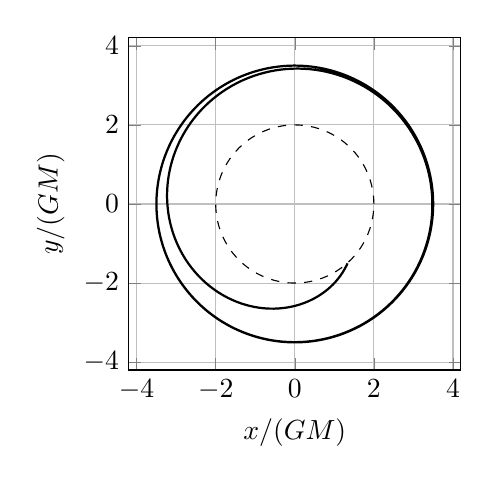
\begin{tikzpicture}\begin{axis}[axis equal image,width=.62\textwidth,height=5.8cm,xlabel={$x/(GM)$},ylabel={$y/(GM)$},grid=major]
\addplot[thick] coordinates {
(3.4999990,0.0000000)
(3.4971422,0.1413829)
(3.4885766,0.2825350)
(3.4743162,0.4232259)
(3.4543841,0.5632259)
(3.4288130,0.7023065)
(3.3976446,0.8402406)
(3.3609297,0.9768031)
(3.3187284,1.1117710)
(3.2711094,1.2449241)
(3.2181506,1.3760448)
(3.1599384,1.5049193)
(3.0965677,1.6313371)
(3.0281422,1.7550918)
(2.9547734,1.8759815)
(2.8765811,1.9938087)
(2.7936930,2.1083812)
(2.7062444,2.2195119)
(2.6143780,2.3270194)
(2.5182438,2.4307282)
(2.4179988,2.5304690)
(2.3138065,2.6260789)
(2.2058371,2.7174020)
(2.0942668,2.8042891)
(1.9792778,2.8865983)
(1.8610577,2.9641954)
(1.7397996,3.0369537)
(1.6157013,3.1047543)
(1.4889656,3.1674866)
(1.3597992,3.2250481)
(1.2284130,3.2773450)
(1.0950215,3.3242919)
(0.9598424,3.3658121)
(0.8230965,3.4018378)
(0.6850069,3.4323102)
(0.5457991,3.4571796)
(0.4057004,3.4764054)
(0.2649393,3.4899561)
(0.1237457,3.4978098)
(-0.0176498,3.4999535)
(-0.1590166,3.4963837)
(-0.3001238,3.4871063)
(-0.4407410,3.4721365)
(-0.5806388,3.4514986)
(-0.7195887,3.4252264)
(-0.8573639,3.3933627)
(-0.9937395,3.3559595)
(-1.1284929,3.3130780)
(-1.2614041,3.2647880)
(-1.3922562,3.2111685)
(-1.5208355,3.1523070)
(-1.6469321,3.0882996)
(-1.7703402,3.0192506)
(-1.8908583,2.9452730)
(-2.0082897,2.8664873)
(-2.1224428,2.7830223)
(-2.2331310,2.6950142)
(-2.3401738,2.6026067)
(-2.4433964,2.5059505)
(-2.5426304,2.4052036)
(-2.6377136,2.3005302)
(-2.7284909,2.1921015)
(-2.8148141,2.0800942)
(-2.8965424,1.9646913)
(-2.9735421,1.8460812)
(-3.0456878,1.7244574)
(-3.1128615,1.6000186)
(-3.1749537,1.4729678)
(-3.2318629,1.3435125)
(-3.2834964,1.2118640)
(-3.3297697,1.0782372)
(-3.3706073,0.9428503)
(-3.4059426,0.8059241)
(-3.4357179,0.6676824)
(-3.4598846,0.5283507)
(-3.4784032,0.3881565)
(-3.4912435,0.2473287)
(-3.4983846,0.1060971)
(-3.4998147,-0.0353077)
(-3.4955316,-0.1766549)
(-3.4855421,-0.3177136)
(-3.4698628,-0.4582538)
(-3.4485190,-0.5980458)
(-3.4215457,-0.7368616)
(-3.3889870,-0.8744745)
(-3.3508958,-1.0106598)
(-3.3073345,-1.1451953)
(-3.2583741,-1.2778613)
(-3.2040946,-1.4084413)
(-3.1445846,-1.5367220)
(-3.0799411,-1.6624941)
(-3.0102698,-1.7855523)
(-2.9356844,-1.9056957)
(-2.8563066,-2.0227280)
(-2.7722660,-2.1364584)
(-2.6836998,-2.2467011)
(-2.5907525,-2.3532761)
(-2.4935760,-2.4560095)
(-2.3923288,-2.5547336)
(-2.2871762,-2.6492871)
(-2.1782898,-2.7395158)
(-2.0658475,-2.8252723)
(-1.9500328,-2.9064167)
(-1.8310347,-2.9828165)
(-1.7090475,-3.0543468)
(-1.5842703,-3.1208911)
(-1.4569068,-3.1823406)
(-1.3271650,-3.2385950)
(-1.1952567,-3.2895625)
(-1.0613971,-3.3351599)
(-0.9258048,-3.3753127)
(-0.7887011,-3.4099554)
(-0.6503099,-3.4390313)
(-0.5108571,-3.4624932)
(-0.3705703,-3.4803026)
(-0.2296786,-3.4924304)
(-0.0884119,-3.4988569)
(0.0529991,-3.4995715)
(0.1943236,-3.4945731)
(0.3353308,-3.4838699)
(0.4757907,-3.4674793)
(0.6154738,-3.4454280)
(0.7541521,-3.4177520)
(0.8915993,-3.3844966)
(1.0275910,-3.3457159)
(1.1619051,-3.3014734)
(1.2943223,-3.2518412)
(1.4246266,-3.1969003)
(1.5526052,-3.1367404)
(1.6780491,-3.0714597)
(1.8007535,-3.0011648)
(1.9205182,-2.9259704)
(2.0371476,-2.8459993)
(2.1504513,-2.7613820)
(2.2602442,-2.6722567)
(2.3663473,-2.5787688)
(2.4685872,-2.4810710)
(2.5667970,-2.3793227)
(2.6608164,-2.2736900)
(2.7504919,-2.1643455)
(2.8356770,-2.0514675)
(2.9162327,-1.9352403)
(2.9920275,-1.8158538)
(3.0629375,-1.6935027)
(3.1288471,-1.5683869)
(3.1896486,-1.4407105)
(3.2452427,-1.3106821)
(3.2955387,-1.1785138)
(3.3404544,-1.0444215)
(3.3799164,-0.9086241)
(3.4138603,-0.7713433)
(3.4422308,-0.6328031)
(3.4649813,-0.4932298)
(3.4820749,-0.3528513)
(3.4934835,-0.2118967)
(3.4991884,-0.0705961)
(3.4991805,0.0708197)
(3.4934595,0.2121199)
(3.4820349,0.3530738)
(3.4649253,0.4934512)
(3.4421586,0.6330230)
(3.4137719,0.7715612)
(3.3798115,0.9088397)
(3.3403329,1.0446344)
(3.2954004,1.1787234)
(3.2450875,1.3108879)
(3.1894762,1.4409121)
(3.1286572,1.5685836)
(3.0627300,1.6936941)
(2.9918019,1.8160390)
(2.9159890,1.9354188)
(2.8354147,2.0516385)
(2.7502109,2.1645082)
(2.6605164,2.2738437)
(2.5664777,2.3794663)
(2.4682483,2.4812036)
(2.3659886,2.5788895)
(2.2598656,2.6723643)
(2.1500524,2.7614755)
(2.0367284,2.8460774)
(1.9200786,2.9260319)
(1.8002934,3.0012083)
(1.6775683,3.0714839)
(1.5521039,3.1367438)
(1.4241048,3.1968814)
(1.2937802,3.2517984)
(1.1613427,3.3014051)
(1.0270087,3.3456204)
(0.8909976,3.3843720)
(0.7535313,3.4175966)
(0.6148344,3.4452398)
(0.4751334,3.4672564)
(0.3346564,3.4836104)
(0.1936329,3.4942748)
(0.0522931,3.4992324)
(-0.0891321,3.4984748)
(-0.2304117,3.4920031)
(-0.3713150,3.4798279)
(-0.5116118,3.4619690)
(-0.6510729,3.4384553)
(-0.7894706,3.4093252)
(-0.9265787,3.3746261)
(-1.0621732,3.3344146)
(-1.1960327,3.2887563)
(-1.3279383,3.2377257)
(-1.4576747,3.1814059)
(-1.5850298,3.1198888)
(-1.7097954,3.0532748)
(-1.8317676,2.9816726)
(-1.9507472,2.9051991)
(-2.0665397,2.8239790)
(-2.1789557,2.7381449)
(-2.2878114,2.6478369)
(-2.3929290,2.5532025)
(-2.4941365,2.4543960)
(-2.5912683,2.3515789)
(-2.6841657,2.2449191)
(-2.7726767,2.1345906)
(-2.8566564,2.0207736)
(-2.9359674,1.9036541)
(-3.0104800,1.7834233)
(-3.0800721,1.6602775)
(-3.1446298,1.5344181)
(-3.2040472,1.4060504)
(-3.2582272,1.2753844)
(-3.3070808,1.1426334)
(-3.3505278,1.0080145)
(-3.3884971,0.8717475)
(-3.4209263,0.7340552)
(-3.4477619,0.5951627)
(-3.4689598,0.4552970)
(-3.4844851,0.3146868)
(-3.4943119,0.1735620)
(-3.4984240,0.0321533)
(-3.4968140,-0.1093080)
(-3.4894844,-0.2505905)
(-3.4764467,-0.3914631)
(-3.4577219,-0.5316953)
(-3.4333400,-0.6710576)
(-3.4033407,-0.8093219)
(-3.3677725,-0.9462620)
(-3.3266932,-1.0816535)
(-3.2801696,-1.2152749)
(-3.2282773,-1.3469072)
(-3.1711007,-1.4763348)
(-3.1087330,-1.6033456)
(-3.0412758,-1.7277315)
(-2.9688390,-1.8492884)
(-2.8915407,-1.9678172)
(-2.8095070,-2.0831233)
(-2.7228717,-2.1950175)
(-2.6317761,-2.3033161)
(-2.5363691,-2.4078414)
(-2.4368063,-2.5084214)
(-2.3332504,-2.6048910)
(-2.2258706,-2.6970915)
(-2.1148423,-2.7848712)
(-2.0003471,-2.8680855)
(-1.8825722,-2.9465973)
(-1.7617102,-3.0202772)
(-1.6379588,-3.0890036)
(-1.5115206,-3.1526629)
(-1.3826025,-3.2111498)
(-1.2514157,-3.2643675)
(-1.1181751,-3.3122276)
(-0.9830990,-3.3546507)
(-0.8464087,-3.3915659)
(-0.7083286,-3.4229116)
(-0.5690850,-3.4486352)
(-0.4289065,-3.4686931)
(-0.2880232,-3.4830511)
(-0.1466665,-3.4916844)
(-0.0050687,-3.4945774)
(0.1365374,-3.4917239)
(0.2779189,-3.4831271)
(0.4188432,-3.4687998)
(0.5590782,-3.4487638)
(0.6983928,-3.4230506)
(0.8365574,-3.3917009)
(0.9733441,-3.3547645)
(1.1085270,-3.3123006)
(1.2418828,-3.2643774)
(1.3731911,-3.2110722)
(1.5022345,-3.1524708)
(1.6287994,-3.0886681)
(1.7526759,-3.0197676)
(1.8736584,-2.9458809)
(1.9915460,-2.8671282)
(2.1061425,-2.7836376)
(2.2172572,-2.6955450)
(2.3247046,-2.6029943)
(2.4283054,-2.5061364)
(2.5278861,-2.4051297)
(2.6232800,-2.3001394)
(2.7143268,-2.1913375)
(2.8008732,-2.0789024)
(2.8827732,-1.9630187)
(2.9598883,-1.8438767)
(3.0320877,-1.7216724)
(3.0992483,-1.5966071)
(3.1612554,-1.4688869)
(3.2180024,-1.3387227)
(3.2693914,-1.2063294)
(3.3153330,-1.0719263)
(3.3557467,-0.9357358)
(3.3905610,-0.7979841)
(3.4197134,-0.6588998)
(3.4431507,-0.5187143)
(3.4608290,-0.3776613)
(3.4727137,-0.2359762)
(3.4787799,-0.0938957)
(3.4790121,0.0483423)
(3.4734043,0.1904991)
(3.4619602,0.3323357)
(3.4446932,0.4736133)
(3.4216261,0.6140934)
(3.3927916,0.7535384)
(3.3582318,0.8917117)
(3.3179983,1.0283785)
(3.2721525,1.1633057)
(3.2207648,1.2962626)
(3.1639152,1.4270212)
(3.1016929,1.5553565)
(3.0341963,1.6810469)
(2.9615326,1.8038745)
(2.8838180,1.9236256)
(2.8011775,2.0400907)
(2.7137445,2.1530655)
(2.6216610,2.2623504)
(2.5250768,2.3677514)
(2.4241502,2.4690805)
(2.3190470,2.5661553)
(2.2099405,2.6588003)
(2.0970115,2.7468463)
(1.9804480,2.8301312)
(1.8604445,2.9085002)
(1.7372024,2.9818060)
(1.6109293,3.0499089)
(1.4818388,3.1126776)
(1.3501502,3.1699888)
(1.2160885,3.2217278)
(1.0798835,3.2677885)
(0.9417702,3.3080739)
(0.8019878,3.3424962)
(0.6607799,3.3709767)
(0.5183940,3.3934464)
(0.3750808,3.4098460)
(0.2310946,3.4201259)
(0.0866925,3.4242466)
(-0.0578662,3.4221787)
(-0.2023198,3.4139031)
(-0.3464048,3.3994110)
(-0.4898563,3.3787042)
(-0.6324084,3.3517948)
(-0.7737943,3.3187060)
(-0.9137471,3.2794714)
(-1.0519996,3.2341355)
(-1.1882854,3.1827536)
(-1.3223383,3.1253922)
(-1.4538938,3.0621284)
(-1.5826884,2.9930506)
(-1.7084608,2.9182578)
(-1.8309518,2.8378605)
(-1.9499047,2.7519799)
(-2.0650658,2.6607485)
(-2.1761850,2.5643096)
(-2.2620041,2.4835125)
(-2.3449541,2.3995655)
(-2.4249123,2.3125572)
(-2.4828449,2.2453479)
(-2.5572781,2.1532093)
(-2.6283926,2.0582765)
(-2.6960735,1.9606551)
(-2.7602083,1.8604551)
(-2.8206870,1.7577911)
(-2.8774024,1.6527821)
(-2.9302498,1.5455515)
(-2.9791273,1.4362273)
(-3.0239364,1.3249419)
(-3.0645812,1.2118322)
(-3.1009694,1.0970396)
(-3.1330120,0.9807099)
(-3.1606233,0.8629933)
(-3.1837214,0.7440448)
(-3.2022284,0.6240236)
(-3.2160698,0.5030935)
(-3.2251757,0.3814229)
(-3.2294801,0.2591849)
(-3.2289215,0.1365569)
(-3.2234428,0.0137212)
(-3.2129919,-0.1091352)
(-3.1975212,-0.2318207)
(-3.1769884,-0.3541388)
(-3.1513566,-0.4758881)
(-3.1205941,-0.5968620)
(-3.0846751,-0.7168492)
(-3.0435796,-0.8356328)
(-2.9972941,-0.9529909)
(-2.9458112,-1.0686958)
(-2.8891305,-1.1825143)
(-2.8272589,-1.2942074)
(-2.7602104,-1.4035299)
(-2.6880070,-1.5102304)
(-2.6106793,-1.6140508)
(-2.5282664,-1.7147262)
(-2.4408167,-1.8119843)
(-2.3483888,-1.9055455)
(-2.2510518,-1.9951218)
(-2.1488860,-2.0804167)
(-2.0419844,-2.1611246)
(-1.9304527,-2.2369303)
(-1.8144113,-2.3075079)
(-1.6939961,-2.3725202)
(-1.6009059,-2.4174176)
(-1.5055125,-2.4588361)
(-1.4406756,-2.4844385)
(-1.3416203,-2.5197083)
(-1.2404852,-2.5510704)
(-1.1373682,-2.5783547)
(-1.0323758,-2.6013851)
(-0.9256239,-2.6199794)
(-0.8172391,-2.6339484)
(-0.7441432,-2.6405949)
(-0.6333503,-2.6464149)
(-0.5213222,-2.6470679)
(-0.4082350,-2.6423346)
(-0.2942820,-2.6319856)
(-0.1796761,-2.6157802)
(-0.0646528,-2.5934656)
(0.0121336,-2.5750642)
(0.1272584,-2.5419679)
(0.2420369,-2.5020172)
(0.3561187,-2.4549012)
(0.4691090,-2.4002884)
(0.5805600,-2.3378245)
(0.6899611,-2.2671287)
(0.7614700,-2.2152235)
(0.8316126,-2.1593481)
(0.9001716,-2.0993653)
(0.9669050,-2.0351298)
(1.0315422,-1.9664872)
(1.0937788,-1.8932737)
(1.1532701,-1.8153142)
(1.2096236,-1.7324220)
(1.2623882,-1.6443970)
(1.3110415,-1.5510250)
(1.3336396,-1.5022626)
};\addplot[domain=0:360,samples=100,dashed] ({2*cos(x)},{2*sin(x)});\end{axis}\end{tikzpicture}
\caption{不稳定圆轨道的向内扰动, $r(0)=3.5-10^{-6}$. 虚线圆为 $r=2$.}\label{fig:ps11-inward}\end{figure}
\begin{figure}[htbp]\centering
\begin{tikzpicture}\begin{axis}[axis equal image,width=.42\textwidth,height=5.8cm,title={全轨道},xlabel={$x/(GM)$},ylabel={$y/(GM)$},grid=major]
\addplot[thick] coordinates {
(3.5000010,0.0000000)
(3.4971442,0.1413828)
(3.4885787,0.2825349)
(3.4743182,0.4232257)
(3.4543862,0.5632256)
(3.4288151,0.7023061)
(3.3976468,0.8402402)
(3.3609320,0.9768026)
(3.3187307,1.1117705)
(3.2711119,1.2449234)
(3.2181532,1.3760441)
(3.1599411,1.5049186)
(3.0965706,1.6313363)
(3.0281452,1.7550910)
(2.9547765,1.8759807)
(2.8765844,1.9938079)
(2.7936965,2.1083804)
(2.7062480,2.2195111)
(2.6143819,2.3270187)
(2.5182479,2.4307275)
(2.4180030,2.5304683)
(2.3138110,2.6260784)
(2.2058418,2.7174015)
(2.0942717,2.8042887)
(1.9792829,2.8865981)
(1.8610630,2.9641954)
(1.7398051,3.0369537)
(1.6157071,3.1047545)
(1.4889716,3.1674870)
(1.3598054,3.2250488)
(1.2284195,3.2773460)
(1.0950282,3.3242931)
(0.9598494,3.3658135)
(0.8231037,3.4018395)
(0.6850143,3.4323123)
(0.5458067,3.4571820)
(0.4057081,3.4764082)
(0.2649473,3.4899594)
(0.1237539,3.4978134)
(-0.0176415,3.4999576)
(-0.1590081,3.4963883)
(-0.3001151,3.4871114)
(-0.4407323,3.4721421)
(-0.5806299,3.4515047)
(-0.7195797,3.4252331)
(-0.8573549,3.3933699)
(-0.9937305,3.3559674)
(-1.1284839,3.3130865)
(-1.2613951,3.2647972)
(-1.3922472,3.2111784)
(-1.5208266,3.1523176)
(-1.6469233,3.0883109)
(-1.7703315,3.0192627)
(-1.8908499,2.9452859)
(-2.0082815,2.8665010)
(-2.1224348,2.7830368)
(-2.2331234,2.6950296)
(-2.3401665,2.6026228)
(-2.4433895,2.5059676)
(-2.5426239,2.4052215)
(-2.6377077,2.3005490)
(-2.7284856,2.1921211)
(-2.8148094,2.0801148)
(-2.8965383,1.9647128)
(-2.9735388,1.8461036)
(-3.0456853,1.7244807)
(-3.1128599,1.6000428)
(-3.1749530,1.4729930)
(-3.2318633,1.3435385)
(-3.2834978,1.2118909)
(-3.3297722,1.0782650)
(-3.3706111,0.9428789)
(-3.4059477,0.8059536)
(-3.4357244,0.6677126)
(-3.4598926,0.5283817)
(-3.4784128,0.3881882)
(-3.4912547,0.2473611)
(-3.4983975,0.1061301)
(-3.4998295,-0.0352741)
(-3.4955482,-0.1766207)
(-3.4855608,-0.3176790)
(-3.4698835,-0.4582187)
(-3.4485419,-0.5980104)
(-3.4215709,-0.7368259)
(-3.3890144,-0.8744386)
(-3.3509257,-1.0106239)
(-3.3073669,-1.1451594)
(-3.2584092,-1.2778256)
(-3.2041323,-1.4084058)
(-3.1446250,-1.5366869)
(-3.0799844,-1.6624595)
(-3.0103161,-1.7855183)
(-2.9357336,-1.9056624)
(-2.8563589,-2.0226957)
(-2.7723214,-2.1364272)
(-2.6837583,-2.2466711)
(-2.5908143,-2.3532476)
(-2.4936411,-2.4559826)
(-2.3923972,-2.5547084)
(-2.2872480,-2.6492640)
(-2.1783650,-2.7394949)
(-2.0659262,-2.8252539)
(-1.9501149,-2.9064009)
(-1.8311202,-2.9828035)
(-1.7091365,-3.0543370)
(-1.5843627,-3.1208847)
(-1.4570027,-3.1823378)
(-1.3272642,-3.2385961)
(-1.1953592,-3.2895678)
(-1.0615028,-3.3351696)
(-0.9259137,-3.3753272)
(-0.7888131,-3.4099749)
(-0.6504249,-3.4390562)
(-0.5109750,-3.4625237)
(-0.3706909,-3.4803391)
(-0.2298017,-3.4924732)
(-0.0885375,-3.4989063)
(0.0528714,-3.4996278)
(0.1941939,-3.4946367)
(0.3351994,-3.4839410)
(0.4756577,-3.4675583)
(0.6153396,-3.4455152)
(0.7540171,-3.4178479)
(0.8914637,-3.3846013)
(1.0274551,-3.3458299)
(1.1617694,-3.3015969)
(1.2941872,-3.2519745)
(1.4244925,-3.1970438)
(1.5524725,-3.1368944)
(1.6779183,-3.0716244)
(1.8006252,-3.0013406)
(1.9203929,-2.9261575)
(2.0370258,-2.8461980)
(2.1503337,-2.7615926)
(2.2601315,-2.6724793)
(2.3662400,-2.5790037)
(2.4684861,-2.4813183)
(2.5667028,-2.3795826)
(2.6607299,-2.2739627)
(2.7504138,-2.1646309)
(2.8356082,-2.0517659)
(2.9161741,-1.9355517)
(2.9919799,-1.8161782)
(3.0629019,-1.6938401)
(3.1288244,-1.5687372)
(3.1896397,-1.4410737)
(3.2452487,-1.3110579)
(3.2955606,-1.1789022)
(3.3404932,-1.0448221)
(3.3799733,-0.9090367)
(3.4139365,-0.7717674)
(3.4423272,-0.6332385)
(3.4650992,-0.4936759)
(3.4822154,-0.3533076)
(3.4936478,-0.2123625)
(3.4993778,-0.0710709)
(3.4993961,0.0703367)
(3.4937027,0.2116296)
(3.4823068,0.3525770)
(3.4652272,0.4929490)
(3.4424917,0.6325163)
(3.4141375,0.7710513)
(3.3802108,0.9083278)
(3.3407671,1.0441218)
(3.2958708,1.1782117)
(3.2455952,1.3103785)
(3.1900224,1.4404066)
(3.1292431,1.5680838)
(3.0633565,1.6932018)
(2.9924703,1.8155563)
(2.9167002,1.9349476)
(2.8361698,2.0511811)
(2.7510106,2.1640668)
(2.6613616,2.2734207)
(2.5673693,2.3790644)
(2.4691869,2.4808254)
(2.3669749,2.5785376)
(2.2609000,2.6720418)
(2.1511354,2.7611852)
(2.0378602,2.8458226)
(1.9212594,2.9258157)
(1.8015232,3.0010342)
(1.6788472,3.0713553)
(1.5534314,3.1366642)
(1.4254807,3.1968546)
(1.2952038,3.2518282)
(1.1628133,3.3014955)
(1.0285254,3.3457753)
(0.8925592,3.3845956)
(0.7551365,3.4178930)
(0.6164816,3.4456133)
(0.4768209,3.4677115)
(0.3363821,3.4841514)
(0.1953944,3.4949063)
(0.0540879,3.4999589)
(-0.0873068,3.4993009)
(-0.2285591,3.4929336)
(-0.3694385,3.4808673)
(-0.5097151,3.4631220)
(-0.6491601,3.4397267)
(-0.7875461,3.4107196)
(-0.9246473,3.3761483)
(-1.0602400,3.3360691)
(-1.1941031,3.2905477)
(-1.3260182,3.2396584)
(-1.4557703,3.1834844)
(-1.5831477,3.1221174)
(-1.7079426,3.0556576)
(-1.8299517,2.9842136)
(-1.9489760,2.9079021)
(-2.0648213,2.8268477)
(-2.1772990,2.7411826)
(-2.2862256,2.6510469)
(-2.3914236,2.5565875)
(-2.4927215,2.4579587)
(-2.5899543,2.3553215)
(-2.6829636,2.2488434)
(-2.7715979,2.1386982)
(-2.8557127,2.0250656)
(-2.9351712,1.9081309)
(-3.0098439,1.7880852)
(-3.0796093,1.6651240)
(-3.1443538,1.5394482)
(-3.2039722,1.4112626)
(-3.2583674,1.2807763)
(-3.3074511,1.1482023)
(-3.3511435,1.0137566)
(-3.3893737,0.8776585)
(-3.4220796,0.7401300)
(-3.4492083,0.6013951)
(-3.4707157,0.4616802)
(-3.4865673,0.3212130)
(-3.4967375,0.1802223)
(-3.5012101,0.0389379)
(-3.4999782,-0.1024098)
(-3.4930442,-0.2435908)
(-3.4804198,-0.3843749)
(-3.4621258,-0.5245329)
(-3.4381927,-0.6638365)
(-3.4086596,-0.8020589)
(-3.3735753,-0.9389751)
(-3.3329973,-1.0743622)
(-3.2869921,-1.2080000)
(-3.2356351,-1.3396708)
(-3.1790104,-1.4691607)
(-3.1172107,-1.5962590)
(-3.0503370,-1.7207590)
(-2.9784988,-1.8424584)
(-2.9018134,-1.9611594)
(-2.8204061,-2.0766692)
(-2.7344100,-2.1888003)
(-2.6439654,-2.2973704)
(-2.5492200,-2.4022036)
(-2.4503285,-2.5031298)
(-2.3474521,-2.5999852)
(-2.2407587,-2.6926130)
(-2.1304223,-2.7808632)
(-2.0166227,-2.8645929)
(-1.8995454,-2.9436666)
(-1.7793812,-3.0179566)
(-1.6563257,-3.0873430)
(-1.5305795,-3.1517137)
(-1.4023471,-3.2109651)
(-1.2718372,-3.2650018)
(-1.1392623,-3.3137370)
(-1.0048378,-3.3570927)
(-0.8687823,-3.3949993)
(-0.7313170,-3.4273966)
(-0.5926651,-3.4542330)
(-0.4530518,-3.4754663)
(-0.3127038,-3.4910632)
(-0.1718488,-3.5009997)
(-0.0307152,-3.5052610)
(0.1104682,-3.5038416)
(0.2514726,-3.4967452)
(0.3920697,-3.4839849)
(0.5320320,-3.4655827)
(0.6711329,-3.4415701)
(0.8091476,-3.4119875)
(0.9458532,-3.3768844)
(1.0810289,-3.3363194)
(1.2144567,-3.2903598)
(1.3459214,-3.2390815)
(1.4752113,-3.1825694)
(1.6021183,-3.1209165)
(1.7264385,-3.0542242)
(1.8479719,-2.9826022)
(1.9665238,-2.9061678)
(2.0819041,-2.8250463)
(2.1939281,-2.7393705)
(2.3024167,-2.6492804)
(2.4071968,-2.5549230)
(2.5081014,-2.4564522)
(2.6049700,-2.3540286)
(2.6976487,-2.2478186)
(2.7859908,-2.1379951)
(2.8698565,-2.0247364)
(2.9491137,-1.9082263)
(3.0236378,-1.7886535)
(3.0933119,-1.6662118)
(3.1580274,-1.5410990)
(3.2176836,-1.4135173)
(3.2721884,-1.2836726)
(3.3214580,-1.1517741)
(3.3654172,-1.0180341)
(3.4039996,-0.8826675)
(3.4371476,-0.7458918)
(3.4648124,-0.6079262)
(3.4869544,-0.4689915)
(3.5035428,-0.3293099)
(3.5145558,-0.1891041)
(3.5199809,-0.0485977)
(3.5198145,0.0919860)
(3.5140620,0.2324237)
(3.5027381,0.3724930)
(3.4858662,0.5119723)
(3.4634788,0.6506415)
(3.4356171,0.7882825)
(3.4023311,0.9246789)
(3.3636797,1.0596171)
(3.3197299,1.1928863)
(3.2705574,1.3242789)
(3.2162461,1.4535907)
(3.1568878,1.5806217)
(3.0925825,1.7051757)
(3.0234375,1.8270614)
(2.9495680,1.9460921)
(2.8710963,2.0620863)
(2.7881516,2.1748680)
(2.7008700,2.2842669)
(2.6093944,2.3901187)
(2.5138734,2.4922652)
(2.4144622,2.5905550)
(2.3113213,2.6848431)
(2.2046166,2.7749917)
(2.0945193,2.8608701)
(1.9812053,2.9423549)
(1.8648548,3.0193302)
(1.7456522,3.0916881)
(1.6237858,3.1593281)
(1.4994471,3.2221581)
(1.3728307,3.2800939)
(1.2441341,3.3330597)
(1.1135570,3.3809877)
(0.9813011,3.4238187)
(0.8475696,3.4615020)
(0.7125673,3.4939953)
(0.5764994,3.5212646)
(0.4395721,3.5432847)
(0.3019914,3.5600388)
(0.1639631,3.5715184)
(0.0256926,3.5777238)
(-0.1126158,3.5786632)
(-0.2507592,3.5743533)
(-0.3885362,3.5648192)
(-0.5257475,3.5500937)
(-0.6621962,3.5302178)
(-0.7976880,3.5052402)
(-0.9320318,3.4752174)
(-1.0650398,3.4402132)
(-1.1965278,3.4002988)
(-1.3263157,3.3555525)
(-1.4542276,3.3060596)
(-1.5800921,3.2519117)
(-1.7037428,3.1932072)
(-1.8250181,3.1300506)
(-1.9437621,3.0625521)
(-2.0598242,2.9908278)
(-2.1730596,2.9149989)
(-2.2833297,2.8351919)
(-2.3905017,2.7515379)
(-2.4944496,2.6641724)
(-2.5950536,2.5732352)
(-2.6922006,2.4788699)
(-2.7857843,2.3812233)
(-2.8757054,2.2804458)
(-2.9618714,2.1766902)
(-3.0441969,2.0701120)
(-3.1226038,1.9608688)
(-3.1970210,1.8491199)
(-3.2673844,1.7350262)
(-3.3336375,1.6187495)
(-3.3957306,1.5004526)
(-3.4536214,1.3802986)
(-3.5072745,1.2584506)
(-3.5566618,1.1350718)
(-3.6017620,1.0103246)
(-3.6425606,0.8843704)
(-3.6790501,0.7573698)
(-3.7112295,0.6294817)
(-3.7441638,0.4750655)
(-3.7709214,0.3198651)
(-3.7819943,0.2420531)
(-3.7995555,0.0861672)
(-3.8110492,-0.0698570)
(-3.8165397,-0.2257716)
(-3.8170486,-0.2776770)
(-3.8146542,-0.4330727)
(-3.8064489,-0.5878093)
(-3.7925319,-0.7416644)
(-3.7866421,-0.7927164)
(-3.7652794,-0.9450653)
(-3.7384706,-1.0960479)
(-3.7063428,-1.2454717)
(-3.6944746,-1.2949014)
(-3.6554648,-1.4419640)
(-3.6114589,-1.5870566)
(-3.5626048,-1.7300192)
(-3.5452690,-1.7771740)
(-3.4901890,-1.9170660)
(-3.4306238,-2.0544950)
(-3.3667349,-2.1893354)
(-3.3445061,-2.2336867)
(-3.2751081,-2.3648977)
(-3.2017727,-2.4932663)
(-3.1246681,-2.6187006)
(-3.0981581,-2.6598455)
(-3.0162907,-2.7812412)
(-2.9310483,-2.8995257)
(-2.8275581,-3.0335127)
(-2.8124330,-3.0522966)
(-2.7042802,-3.1812545)
(-2.5923289,-3.3057458)
(-2.4935435,-3.4088624)
(-2.3752202,-3.5249483)
(-2.2538240,-3.6364756)
(-2.1475086,-3.7284377)
(-2.0210452,-3.8314941)
(-1.8921850,-3.9300090)
(-1.7799948,-4.0108567)
(-1.6472681,-4.1010198)
(-1.5127592,-4.1867484)
(-1.3961983,-4.2567420)
(-1.2391814,-4.3451302)
(-1.0805812,-4.4279720)
(-1.0007681,-4.4673485)
(-0.8402687,-4.5420885)
(-0.6787980,-4.6115851)
(-0.5977671,-4.6444091)
(-0.4352436,-4.7062955)
(-0.2722661,-4.7632866)
(-0.1906643,-4.7899923)
(-0.0069213,-4.8458373)
(0.1768317,-4.8959841)
(0.2176459,-4.9063759)
(0.4011331,-4.9498546)
(0.5841995,-4.9881212)
(0.6248071,-4.9959391)
(0.8273551,-5.0314126)
(1.0289499,-5.0610759)
(1.2294245,-5.0852197)
(1.4286353,-5.1041279)
(1.6461620,-5.1192094)
(1.8227954,-5.1273346)
(2.0369434,-5.1324080)
(2.2106746,-5.1328009)
(2.4401714,-5.1283829)
(2.5917760,-5.1224760)
(2.8170563,-5.1094506)
(2.9658114,-5.0981444)
(3.1867841,-5.0775019)
(3.3326580,-5.0614236)
(3.5493133,-5.0340562)
(3.6923215,-5.0137686)
(3.9047112,-4.9804740)
(4.0449046,-4.9564791)
(4.2531260,-4.9179673)
(4.3905814,-4.8907107)
(4.5947642,-4.8476104)
(4.7295762,-4.8174861)
(4.9298722,-4.7703523)
(5.0621473,-4.7377075)
(5.2587220,-4.6870290)
(5.3885734,-4.6521691)
(5.5815999,-4.5983751)
(5.7091444,-4.5615682)
(5.8987982,-4.5050355)
(6.0241527,-4.4665168)
(6.2106085,-4.4075755)
(6.3338884,-4.3675510)
(6.5173173,-4.3064905)
(6.6386350,-4.2651406)
(6.8341752,-4.1969239)
(6.9386665,-4.1596973)
(7.1312834,-4.0897054)
(7.2342455,-4.0515816)
(7.4241032,-3.9800248)
(7.5256220,-3.9411098)
(7.7128760,-3.8681723)
(7.8130331,-3.8285590)
(7.9978303,-3.7544027)
(8.0967023,-3.7141727)
(8.2931577,-3.6331258)
(8.3768402,-3.5981648)
(8.5709419,-3.5160962)
(8.6536444,-3.4807236)
(8.8455233,-3.3977514)
(8.9272998,-3.3620146)
(9.1170785,-3.2782430)
(9.1979800,-3.2421841)
(9.3857729,-3.1577051)
(9.4658467,-3.1213609)
(9.6649919,-3.0301613)
(9.7310515,-2.9996592)
(9.9282935,-2.9078674)
(9.9937356,-2.8771797)
(10.1891744,-2.7848639)
(10.2540313,-2.7540120)
(10.4477601,-2.6612326)
(10.5120618,-2.6302353)
(10.7169330,-2.5308232)
(10.7679424,-2.5059203)
(10.9711716,-2.4061229)
(11.0217808,-2.3811295)
(11.2234490,-2.2809921)
(11.2736777,-2.2559189)
(11.4738608,-2.1554818)
(11.5237272,-2.1303382)
(11.7348828,-2.0233372)
(11.7720175,-2.0044321)
(11.9817429,-1.8971858)
(12.0186311,-1.8782402)
(12.2269923,-1.7707791)
(12.2636454,-1.7517981)
(12.4707044,-1.6441495)
(12.5071329,-1.6251377)
(12.7250226,-1.5109804)
(12.7491617,-1.4982876)
(12.9657934,-1.3839815)
(12.9897958,-1.3712733)
(13.2052236,-1.2568393)
(13.2290952,-1.2441180)
(13.4433703,-1.1295748)
(13.4671164,-1.1168424)
(13.6921013,-0.9958361)
(13.7039128,-0.9894651)
(13.9277805,-0.8683777)
(13.9395344,-0.8620028)
(14.1623300,-0.7408487)
(14.1740286,-0.7344706)
(14.4074400,-0.6068823)
(14.6398106,-0.4792500)
(14.8711805,-0.3515849)
(15.1015871,-0.2238970)
(15.3310663,-0.0961952)
(15.5596518,0.0315123)
(15.7873757,0.1592180)
(16.0142683,0.2869155)
(16.2403585,0.4145986)
(16.4656738,0.5422620)
(16.6902403,0.6699007)
(16.9140827,0.7975105)
(17.1372247,0.9250872)
(17.3596889,1.0526274)
(17.5814967,1.1801278)
(17.8026685,1.3075856)
(18.0232240,1.4349981)
(18.2431818,1.5623631)
(18.4625597,1.6896784)
(18.6813750,1.8169423)
(18.8996438,1.9441530)
(19.1173819,2.0713092)
(19.3346042,2.1984095)
(19.5513252,2.3254528)
(19.7675585,2.4524381)
(19.9833175,2.5793646)
(20.1986148,2.7062315)
(20.4134627,2.8330382)
(20.6278728,2.9597842)
(20.8418565,3.0864690)
(21.0554246,3.2130922)
(21.2685875,3.3396537)
(21.4813552,3.4661531)
(21.6937375,3.5925903)
(21.9057438,3.7189652)
(22.1173828,3.8452778)
(22.3286635,3.9715282)
(22.5395941,4.0977162)
(22.7501827,4.2238421)
(22.9604372,4.3499060)
(23.1703650,4.4759080)
(23.3799735,4.6018483)
(23.5892697,4.7277271)
(23.7982604,4.8535447)
(24.0069522,4.9793014)
(24.2153516,5.1049974)
(24.4234646,5.2306331)
(24.6312972,5.3562087)
(24.8388554,5.4817246)
(25.0461445,5.6071812)
(25.2531703,5.7325788)
(25.4599378,5.8579178)
(25.6664523,5.9831985)
(25.8727186,6.1084214)
(26.0787417,6.2335869)
(26.2845262,6.3586954)
(26.4900767,6.4837473)
(26.6953975,6.6087429)
(26.9004931,6.7336828)
(27.1053675,6.8585674)
(27.3100248,6.9833970)
(27.5144689,7.1081721)
(27.7187038,7.2328931)
(27.9227331,7.3575605)
(28.1265605,7.4821747)
(28.3301896,7.6067362)
(28.5336237,7.7312452)
(28.7368662,7.8557024)
(28.9399204,7.9801081)
(29.1427895,8.1044628)
(29.3454765,8.2287669)
(29.5479846,8.3530207)
(29.7503167,8.4772248)
(29.9524756,8.6013796)
(30.1544642,8.7254854)
(30.3562851,8.8495428)
(30.5579411,8.9735521)
(30.7594348,9.0975137)
(30.9607687,9.2214280)
(31.1619454,9.3452955)
(31.3629671,9.4691166)
(31.5638364,9.5928916)
(31.7645555,9.7166210)
(31.9651267,9.8403051)
(32.1655522,9.9639444)
(32.3658342,10.0875393)
(32.5659748,10.2110900)
(32.7659760,10.3345971)
(32.9658399,10.4580609)
(33.1655685,10.5814817)
(33.3651636,10.7048599)
(33.5646273,10.8281960)
(33.7639613,10.9514902)
(33.9631674,11.0747430)
(34.1622475,11.1979547)
(34.3612032,11.3211256)
(34.5600364,11.4442561)
(34.7587485,11.5673466)
(34.9573413,11.6903973)
(35.1558164,11.8134087)
(35.3541754,11.9363810)
(35.5524197,12.0593147)
(35.7505509,12.1822100)
(35.9485705,12.3050672)
(36.1464799,12.4278867)
(36.3442805,12.5506688)
(36.5419737,12.6734139)
(36.7395609,12.7961222)
(36.9370434,12.9187940)
(37.1344226,13.0414296)
(37.3316996,13.1640294)
(37.5288759,13.2865937)
(37.7259525,13.4091227)
(37.9229309,13.5316167)
(38.1198120,13.6540761)
(38.3165972,13.7765011)
(38.5132875,13.8988920)
(38.7098841,14.0212491)
(38.9063881,14.1435726)
(39.1028006,14.2658629)
(39.2991227,14.3881202)
(39.4953553,14.5103447)
(39.6914997,14.6325368)
(39.8875566,14.7546967)
(40.0835273,14.8768246)
(40.2794126,14.9989209)
(40.4752135,15.1209858)
(40.6709309,15.2430194)
(40.8665658,15.3650222)
(41.0621192,15.4869943)
(41.2575918,15.6089359)
(41.4529846,15.7308473)
(41.6482985,15.8527288)
(41.8435343,15.9745806)
(42.0386928,16.0964028)
(42.2337750,16.2181958)
(42.4287815,16.3399598)
(42.6237132,16.4616950)
(42.8185710,16.5834016)
(43.0133555,16.7050798)
(43.2080675,16.8267299)
(43.4027078,16.9483521)
(43.5972771,17.0699465)
(43.7917762,17.1915134)
(43.9862058,17.3130531)
(44.1805665,17.4345656)
(44.3748592,17.5560513)
(44.5690843,17.6775103)
(44.7632427,17.7989428)
(44.9573351,17.9203491)
(45.1513619,18.0417292)
(45.3453240,18.1630834)
(45.5392219,18.2844120)
(45.7330563,18.4057150)
(45.9268277,18.5269927)
(46.1205368,18.6482453)
(46.3141842,18.7694729)
(46.5077705,18.8906758)
(46.7012963,19.0118540)
(46.8947620,19.1330079)
(47.0881684,19.2541375)
(47.2815159,19.3752430)
(47.4748051,19.4963247)
(47.6680365,19.6173826)
(47.8612108,19.7384170)
(48.0543283,19.8594280)
(48.2473896,19.9804158)
(48.4403953,20.1013805)
(48.6333458,20.2223223)
(48.8262416,20.3432414)
(49.0190833,20.4641379)
(49.2118713,20.5850121)
(49.4046060,20.7058639)
(49.5972880,20.8266937)
(49.7899178,20.9475015)
(49.9824957,21.0682875)
(50.1750223,21.1890518)
(50.3674979,21.3097947)
(50.5599231,21.4305161)
(50.7522982,21.5512164)
(50.9446237,21.6718956)
(51.1369000,21.7925539)
(51.3291276,21.9131914)
(51.5213068,22.0338083)
(51.7134380,22.1544046)
(51.9055217,22.2749806)
(52.0975583,22.3955364)
(52.2895480,22.5160720)
(52.4814915,22.6365877)
(52.6733889,22.7570836)
(52.8652407,22.8775597)
(53.0570473,22.9980163)
(53.2488091,23.1184534)
(53.4405263,23.2388712)
(53.6321994,23.3592698)
(53.8238287,23.4796493)
(54.0154145,23.6000099)
(54.2069573,23.7203517)
(54.3984573,23.8406747)
(54.5899150,23.9609792)
(54.7813305,24.0812652)
(54.9727043,24.2015329)
(55.1640367,24.3217823)
(55.3553280,24.4420136)
(55.5465785,24.5622269)
(55.7377885,24.6824223)
(55.9289584,24.8025999)
(56.1200885,24.9227598)
(56.3111790,25.0429022)
(56.5022303,25.1630272)
(56.6932426,25.2831348)
(56.8842163,25.4032252)
(57.0751517,25.5232984)
(57.2660490,25.6433546)
(57.4569085,25.7633939)
(57.6477305,25.8834164)
(57.8385152,26.0034222)
(58.0292630,26.1234113)
(58.2199742,26.2433840)
(58.4106489,26.3633402)
(58.6012875,26.4832801)
(58.7918902,26.6032038)
(58.9824572,26.7231114)
(59.1729889,26.8430030)
(59.3634855,26.9628786)
(59.5539472,27.0827384)
(59.7443744,27.2025825)
(59.9347671,27.3224109)
(60.1251257,27.4422237)
(60.3154505,27.5620211)
(60.5057416,27.6818031)
(60.6959993,27.8015698)
(60.8862238,27.9213214)
(61.0764153,28.0410578)
(61.2665742,28.1607792)
(61.4567005,28.2804857)
(61.6467946,28.4001773)
(61.8368566,28.5198541)
(62.0268869,28.6395163)
(62.2168855,28.7591639)
(62.4068526,28.8787969)
(62.5967887,28.9984156)
(62.7866937,29.1180199)
(62.9765680,29.2376099)
(63.1664117,29.3571857)
(63.3562250,29.4767474)
(63.5460082,29.5962951)
(63.7357615,29.7158288)
(63.9254849,29.8353487)
(64.1151788,29.9548547)
(64.3048434,30.0743471)
(64.4944787,30.1938258)
(64.6840851,30.3132909)
(64.8736627,30.4327425)
(65.0632116,30.5521807)
(65.2527322,30.6716056)
(65.4422245,30.7910171)
(65.6316887,30.9104155)
(65.8211250,31.0298007)
(66.0105336,31.1491729)
(66.1999147,31.2685321)
(66.3892684,31.3878783)
(66.5785950,31.5072117)
(66.7678945,31.6265324)
(66.9571671,31.7458402)
(67.1464131,31.8651355)
(67.3356326,31.9844182)
(67.5248257,32.1036883)
(67.7139926,32.2229460)
(67.9031335,32.3421913)
(68.0922486,32.4614243)
(68.2813379,32.5806450)
(68.4704017,32.6998536)
(68.6594400,32.8190500)
(68.8484532,32.9382343)
(69.0374412,33.0574067)
(69.2264043,33.1765670)
(69.4153426,33.2957156)
(69.6042563,33.4148523)
(69.7931455,33.5339772)
(69.9820103,33.6530904)
(70.1708509,33.7721920)
(70.3596675,33.8912821)
(70.5484601,34.0103606)
(70.7372290,34.1294276)
(70.9259742,34.2484832)
(71.1146959,34.3675275)
(71.3033943,34.4865605)
(71.4920694,34.6055823)
(71.6807214,34.7245928)
(71.8693505,34.8435923)
(72.0579568,34.9625807)
(72.2465403,35.0815580)
(72.4351013,35.2005245)
(72.6236398,35.3194800)
(72.8121561,35.4384246)
(73.0006501,35.5573585)
(73.1891221,35.6762816)
(73.3775721,35.7951940)
(73.5660004,35.9140958)
(73.7544069,36.0329870)
(73.9427919,36.1518677)
(74.1311554,36.2707378)
(74.3194976,36.3895976)
(74.5078186,36.5084469)
(74.6961185,36.6272859)
(74.8843974,36.7461147)
(75.0726555,36.8649331)
(75.2608928,36.9837414)
(75.4491095,37.1025396)
(75.6373056,37.2213277)
(75.8254814,37.3401057)
(76.0136368,37.4588737)
(76.2017721,37.5776318)
(76.3898873,37.6963800)
(76.5779825,37.8151183)
(76.7660578,37.9338468)
(76.9541134,38.0525656)
(77.1421493,38.1712746)
(77.3301657,38.2899740)
(77.5181626,38.4086637)
(77.7061402,38.5273438)
(77.8940985,38.6460144)
(78.0820377,38.7646755)
(78.2699579,38.8833272)
(78.4578591,39.0019694)
(78.6457414,39.1206023)
(78.8336051,39.2392259)
(79.0214500,39.3578401)
(79.2092765,39.4764452)
(79.3970845,39.5950410)
(79.5848741,39.7136277)
(79.7726454,39.8322052)
(79.9603986,39.9507737)
(80.1481337,40.0693332)
(80.3358508,40.1878837)
(80.5235500,40.3064252)
(80.7112315,40.4249578)
(80.8988952,40.5434815)
(81.0865412,40.6619964)
(81.2741698,40.7805025)
(81.4617809,40.8989998)
(81.6493746,41.0174885)
(81.8369510,41.1359684)
(82.0245103,41.2544397)
(82.2120524,41.3729024)
(82.3995776,41.4913566)
(82.5870858,41.6098022)
(82.7745771,41.7282393)
(82.9620517,41.8466680)
(83.1495096,41.9650882)
(83.3369509,42.0835001)
(83.5243757,42.2019036)
(83.7117840,42.3202989)
(83.8991759,42.4386858)
(84.0865516,42.5570645)
(84.2739111,42.6754350)
(84.4612544,42.7937974)
(84.6485817,42.9121516)
(84.8358930,43.0304977)
(85.0231884,43.1488357)
(85.2104680,43.2671657)
(85.3977319,43.3854878)
(85.5849800,43.5038018)
(85.7722126,43.6221080)
(85.9594297,43.7404062)
(86.1466313,43.8586966)
(86.3338175,43.9769791)
(86.5209884,44.0952539)
(86.7081441,44.2135208)
(86.8952846,44.3317801)
(87.0824100,44.4500316)
(87.2695205,44.5682755)
(87.4566159,44.6865118)
(87.6436965,44.8047404)
(87.8307622,44.9229615)
(88.0178132,45.0411750)
(88.2048495,45.1593810)
(88.3918713,45.2775795)
(88.5788784,45.3957706)
(88.7658711,45.5139543)
(88.9528494,45.6321306)
(89.1398133,45.7502995)
(89.3267630,45.8684610)
(89.5136984,45.9866153)
(89.7006197,46.1047623)
(89.8875268,46.2229021)
(90.0744200,46.3410346)
(90.2612992,46.4591600)
(90.4481644,46.5772782)
(90.6350159,46.6953893)
(90.8218536,46.8134933)
(91.0086775,46.9315902)
(91.1954878,47.0496801)
(91.3822845,47.1677629)
(91.5690676,47.2858388)
(91.7558373,47.4039077)
(91.9425935,47.5219697)
(92.1293364,47.6400247)
(92.3160660,47.7580729)
(92.5027824,47.8761143)
(92.6894855,47.9941488)
(92.8761756,48.1121765)
(93.0628525,48.2301974)
(93.2495165,48.3482116)
(93.4361675,48.4662191)
(93.6228055,48.5842199)
(93.8094308,48.7022140)
(93.9960432,48.8202015)
(94.1826429,48.9381823)
(94.3692299,49.0561566)
(94.5558043,49.1741243)
(94.7423661,49.2920854)
(94.9289154,49.4100401)
(95.1154522,49.5279882)
(95.3019766,49.6459299)
(95.4884886,49.7638652)
(95.6749883,49.8817940)
(95.8614757,49.9997164)
(96.0479510,50.1176325)
(96.2344140,50.2355422)
(96.4208650,50.3534456)
(96.6073039,50.4713427)
(96.7937308,50.5892335)
(96.9801457,50.7071181)
(97.1665487,50.8249964)
(97.3529398,50.9428685)
(97.5393192,51.0607345)
(97.7256867,51.1785943)
(97.9120426,51.2964479)
(98.0983868,51.4142955)
(98.2847193,51.5321369)
(98.4710403,51.6499723)
(98.6573498,51.7678016)
(98.8436478,51.8856249)
(99.0299343,52.0034423)
(99.2162094,52.1212536)
(99.4024733,52.2390590)
(99.5887258,52.3568584)
(99.7749670,52.4746519)
(99.9611971,52.5924395)
(100.1474160,52.7102213)
(100.3336237,52.8279972)
(100.5198204,52.9457672)
(100.7060061,53.0635315)
(100.8921808,53.1812900)
(101.0783445,53.2990427)
(101.2644974,53.4167896)
(101.4506393,53.5345308)
(101.6367705,53.6522664)
(101.8228909,53.7699962)
(102.0090006,53.8877204)
(102.1950996,54.0054389)
(102.3811879,54.1231518)
(102.5672656,54.2408591)
(102.7533328,54.3585608)
(102.9393894,54.4762569)
(103.1254356,54.5939475)
(103.3114713,54.7116325)
(103.4974966,54.8293121)
(103.6835115,54.9469862)
(103.8695162,55.0646547)
(104.0555105,55.1823179)
(104.2414946,55.2999756)
(104.4274685,55.4176279)
(104.6134323,55.5352748)
(104.7993859,55.6529163)
(104.9853294,55.7705525)
(105.1712628,55.8881833)
(105.3571863,56.0058088)
(105.5430998,56.1234290)
(105.7290033,56.2410439)
(105.9148970,56.3586536)
(106.1007807,56.4762580)
(106.2866547,56.5938572)
(106.4725189,56.7114511)
(106.6583733,56.8290399)
(106.8442180,56.9466235)
(107.0300530,57.0642019)
(107.2158784,57.1817752)
(107.4016941,57.2993434)
(107.5875003,57.4169064)
(107.7732970,57.5344644)
(107.9590841,57.6520173)
(108.1448618,57.7695651)
(108.3306300,57.8871079)
(108.5163889,58.0046457)
(108.7021383,58.1221785)
(108.8878785,58.2397063)
(109.0736093,58.3572291)
(109.2593309,58.4747469)
(109.4450433,58.5922598)
(109.6307464,58.7097678)
(109.8164404,58.8272709)
(110.0021253,58.9447691)
(110.1878011,59.0622624)
(110.3734678,59.1797508)
(110.5591254,59.2972345)
(110.7447741,59.4147132)
(110.9304138,59.5321872)
(111.1160446,59.6496564)
(111.3016664,59.7671208)
(111.4872794,59.8845804)
(111.6728836,60.0020353)
(111.8584789,60.1194855)
(112.0440655,60.2369309)
(112.2296433,60.3543716)
(112.4152124,60.4718077)
(112.6007728,60.5892390)
(112.7863245,60.7066657)
(112.9718676,60.8240878)
(113.1574022,60.9415052)
(113.3429281,61.0589181)
(113.5284456,61.1763263)
(113.7139545,61.2937299)
(113.8994549,61.4111290)
(114.0849469,61.5285235)
(114.2704305,61.6459135)
(114.4559057,61.7632990)
(114.6413725,61.8806799)
(114.8268310,61.9980563)
(115.0122812,62.1154283)
(115.1977231,62.2327958)
(115.3831568,62.3501588)
(115.5685822,62.4675174)
(115.7539995,62.5848716)
(115.9394086,62.7022213)
(116.1248095,62.8195667)
(116.3102024,62.9369077)
(116.4955872,63.0542443)
(116.6809639,63.1715765)
(116.8663326,63.2889044)
(117.0516933,63.4062280)
(117.2370460,63.5235472)
(117.4223908,63.6408622)
(117.6077277,63.7581728)
(117.7930566,63.8754792)
(117.9783777,63.9927813)
(118.1636910,64.1100791)
(118.3489964,64.2273727)
(118.5342941,64.3446621)
(118.7195840,64.4619473)
(118.9048662,64.5792283)
(119.0901406,64.6965051)
(119.2754074,64.8137777)
(119.4606665,64.9310461)
(119.6459180,65.0483104)
(119.8311619,65.1655706)
(120.0163982,65.2828266)
(120.2016269,65.4000785)
(120.3868481,65.5173264)
(120.5720618,65.6345701)
(120.7572680,65.7518098)
(120.9424667,65.8690454)
(121.1276580,65.9862769)
(121.3128419,66.1035044)
(121.4980184,66.2207279)
(121.6831875,66.3379474)
(121.8683493,66.4551629)
(122.0535038,66.5723743)
(122.2386509,66.6895818)
(122.4237908,66.8067854)
(122.6089235,66.9239849)
(122.7940489,67.0411806)
(122.9791671,67.1583723)
(123.1642782,67.2755601)
(123.3493821,67.3927439)
(123.5344788,67.5099239)
(123.7195685,67.6271000)
(123.9046510,67.7442722)
(124.0897265,67.8614406)
(124.2747950,67.9786051)
(124.4598564,68.0957657)
(124.6449109,68.2129225)
(124.8299583,68.3300756)
(125.0149988,68.4472248)
(125.2000324,68.5643702)
(125.3850590,68.6815118)
(125.5700788,68.7986496)
(125.7550917,68.9157837)
(125.9400977,69.0329140)
(126.1250969,69.1500406)
(126.3100893,69.2671635)
(126.4950750,69.3842826)
(126.6800538,69.5013981)
(126.8650260,69.6185098)
(127.0499914,69.7356178)
(127.2349501,69.8527222)
(127.4199021,69.9698229)
(127.6048474,70.0869199)
(127.7897862,70.2040133)
(127.9747183,70.3211031)
(128.1596438,70.4381892)
(128.3445627,70.5552717)
(128.5294751,70.6723506)
(128.7143809,70.7894259)
(128.8992802,70.9064976)
(129.0841730,71.0235658)
(129.2690593,71.1406304)
(129.4539392,71.2576914)
(129.6388126,71.3747489)
(129.8236796,71.4918028)
(130.0085402,71.6088533)
(130.1933944,71.7259002)
(130.3782423,71.8429436)
(130.5630838,71.9599835)
(130.7479190,72.0770199)
(130.9327479,72.1940529)
(131.1175705,72.3110823)
(131.3023868,72.4281083)
(131.4871968,72.5451309)
(131.6720007,72.6621500)
(131.8567983,72.7791658)
(132.0415897,72.8961780)
(132.2263750,73.0131869)
(132.4111541,73.1301924)
(132.5959270,73.2471945)
(132.7806939,73.3641932)
(132.9654546,73.4811885)
(133.1502092,73.5981804)
(133.3349578,73.7151690)
(133.5197003,73.8321543)
(133.7044368,73.9491362)
(133.8891673,74.0661148)
(134.0738917,74.1830901)
(134.2586102,74.3000621)
(134.4433227,74.4170307)
(134.6280293,74.5339961)
(134.8127299,74.6509582)
(134.9974247,74.7679170)
(135.1821135,74.8848726)
(135.3667965,75.0018249)
(135.5514736,75.1187739)
(135.7361448,75.2357197)
(135.9208102,75.3526623)
(136.1054699,75.4696017)
(136.2901237,75.5865378)
(136.4747717,75.7034708)
(136.6594140,75.8204005)
(136.8440505,75.9373271)
(137.0286813,76.0542504)
(137.2133064,76.1711707)
(137.3979258,76.2880877)
(137.5825395,76.4050016)
(137.7671476,76.5219123)
(137.9517500,76.6388199)
(138.1363467,76.7557244)
(138.3209379,76.8726258)
(138.5055234,76.9895240)
(138.6901034,77.1064192)
(138.8746778,77.2233112)
(139.0592466,77.3402002)
(139.2438099,77.4570860)
(139.4283677,77.5739688)
(139.6129200,77.6908486)
(139.7974667,77.8077252)
(139.9820080,77.9245989)
(140.1665439,78.0414695)
(140.3510743,78.1583370)
(140.5355992,78.2752016)
(140.7201188,78.3920631)
(140.9046329,78.5089216)
(141.0891417,78.6257771)
(141.2736450,78.7426296)
(141.4581431,78.8594791)
(141.6426357,78.9763257)
(141.8271231,79.0931692)
(142.0116051,79.2100099)
(142.1960819,79.3268475)
(142.3805533,79.4436822)
(142.5650195,79.5605140)
(142.7494804,79.6773428)
(142.9339361,79.7941687)
(143.1183866,79.9109917)
(143.3028318,80.0278118)
(143.4872718,80.1446290)
(143.6717067,80.2614433)
(143.8561364,80.3782546)
(144.0405609,80.4950632)
(144.2249803,80.6118688)
(144.4093945,80.7286716)
(144.5938037,80.8454715)
(144.7782077,80.9622685)
(144.9626067,81.0790627)
(145.1470005,81.1958541)
(145.3313894,81.3126426)
(145.5157731,81.4294283)
(145.7001518,81.5462112)
(145.8845255,81.6629913)
(146.0688942,81.7797686)
(146.2532579,81.8965431)
(146.4376167,82.0133148)
(146.6219704,82.1300837)
(146.8063192,82.2468498)
(146.9906631,82.3636132)
(147.1750020,82.4803738)
(147.3593360,82.5971317)
(147.5436651,82.7138868)
(147.7279893,82.8306391)
(147.9123087,82.9473888)
(148.0966231,83.0641356)
(148.2809328,83.1808798)
(148.4652375,83.2976213)
(148.6495375,83.4143600)
(148.8338326,83.5310961)
(149.0181230,83.6478294)
(149.2024085,83.7645601)
(149.3866893,83.8812881)
(149.5709653,83.9980134)
(149.7552366,84.1147361)
(149.9395031,84.2314560)
(150.1237648,84.3481734)
(150.3080219,84.4648880)
(150.4922743,84.5816001)
(150.6765220,84.6983094)
(150.8607649,84.8150162)
(151.0450033,84.9317203)
(151.2292369,85.0484219)
(151.4134660,85.1651208)
(151.5976904,85.2818171)
(151.7819101,85.3985108)
(151.9661253,85.5152019)
(152.1503359,85.6318904)
(152.3345418,85.7485764)
(152.5187433,85.8652597)
(152.7029401,85.9819405)
(152.8871324,86.0986188)
(153.0713202,86.2152945)
(153.2555034,86.3319676)
(153.4396821,86.4486382)
(153.6238563,86.5653062)
(153.8080260,86.6819717)
(153.9921913,86.7986347)
(154.1763520,86.9152952)
(154.3605083,87.0319532)
(154.5446602,87.1486086)
(154.7288076,87.2652616)
(154.9129506,87.3819120)
(155.0970891,87.4985600)
(155.2812233,87.6152054)
(155.4653531,87.7318484)
(155.6494785,87.8484890)
(155.8335995,87.9651270)
(156.0177162,88.0817626)
(156.2018285,88.1983957)
(156.3859364,88.3150264)
(156.5700401,88.4316547)
(156.7541394,88.5482805)
(156.9382344,88.6649038)
(157.1223251,88.7815248)
(157.3064115,88.8981433)
(157.4904937,89.0147594)
(157.6745716,89.1313731)
(157.8586452,89.2479844)
(158.0427146,89.3645933)
(158.2267798,89.4811998)
(158.4108407,89.5978039)
(158.5948974,89.7144056)
(158.7789499,89.8310049)
(158.9629982,89.9476019)
(159.1470424,90.0641965)
(159.3310823,90.1807887)
(159.5151181,90.2973786)
(159.6991498,90.4139661)
(159.8831773,90.5305513)
(160.0672006,90.6471342)
(160.2512199,90.7637147)
(160.4352350,90.8802929)
(160.6192460,90.9968687)
(160.8032530,91.1134423)
(160.9872558,91.2300135)
(161.1712546,91.3465824)
(161.3552493,91.4631490)
(161.5392399,91.5797133)
(161.7232266,91.6962753)
(161.9072091,91.8128351)
(162.0911877,91.9293925)
(162.2751622,92.0459477)
(162.4591327,92.1625006)
(162.6430993,92.2790512)
(162.8270618,92.3955996)
(163.0110204,92.5121457)
(163.1949749,92.6286895)
(163.3789256,92.7452311)
(163.5628723,92.8617705)
(163.7468150,92.9783076)
(163.9307538,93.0948425)
(164.1146887,93.2113752)
(164.2986197,93.3279057)
(164.4825467,93.4444339)
(164.6664699,93.5609599)
(164.8503892,93.6774837)
(165.0343046,93.7940053)
(165.2182161,93.9105247)
(165.4021238,94.0270419)
(165.5860276,94.1435569)
(165.7699276,94.2600698)
(165.9538238,94.3765804)
(166.1377161,94.4930889)
(166.3216046,94.6095952)
(166.5054893,94.7260994)
(166.6893703,94.8426014)
(166.8732474,94.9591012)
(167.0571207,95.0755989)
(167.2409903,95.1920944)
(167.4248561,95.3085878)
(167.6087182,95.4250791)
(167.7925765,95.5415682)
(167.9764311,95.6580552)
(168.1602819,95.7745401)
(168.3441290,95.8910228)
(168.5279725,96.0075035)
(168.7118122,96.1239820)
(168.8956482,96.2404584)
(169.0794805,96.3569328)
(169.2633092,96.4734050)
(169.4471342,96.5898751)
(169.6309555,96.7063432)
(169.8147732,96.8228092)
(169.9985872,96.9392731)
(170.1823976,97.0557349)
(170.3662043,97.1721946)
(170.5500075,97.2886523)
(170.7338070,97.4051079)
(170.9176030,97.5215615)
(171.1013953,97.6380130)
(171.2851840,97.7544625)
(171.4689692,97.8709099)
(171.6527508,97.9873553)
(171.8365288,98.1037987)
(172.0203033,98.2202400)
(172.2040742,98.3366793)
(172.3878416,98.4531166)
(172.5716055,98.5695518)
(172.7553658,98.6859851)
(172.9391226,98.8024163)
(173.1228759,98.9188455)
(173.3066257,99.0352728)
(173.4903720,99.1516980)
(173.6741149,99.2681213)
(173.8578542,99.3845425)
(174.0415901,99.5009618)
(174.2253225,99.6173791)
(174.4090515,99.7337944)
(174.5927770,99.8502078)
(174.7764991,99.9666191)
(174.9602177,100.0830286)
(175.1439329,100.1994360)
(175.3276447,100.3158415)
(175.5113531,100.4322451)
(175.6950581,100.5486467)
(175.8787597,100.6650464)
(176.0624579,100.7814441)
(176.2461528,100.8978399)
(176.4298442,101.0142337)
(176.6135323,101.1306257)
(176.7972170,101.2470157)
(176.9808984,101.3634038)
(177.1645765,101.4797899)
(177.3482512,101.5961742)
(177.5319225,101.7125566)
(177.7155906,101.8289370)
(177.8992553,101.9453156)
(178.0829167,102.0616922)
(178.2665749,102.1780670)
(178.4502297,102.2944399)
(178.6338812,102.4108109)
(178.8175295,102.5271800)
(179.0011745,102.6435472)
(179.1848162,102.7599126)
(179.3684547,102.8762761)
(179.5520899,102.9926377)
(179.7357219,103.1089975)
(179.9193506,103.2253554)
(180.1029761,103.3417115)
(180.2865984,103.4580657)
(180.4702175,103.5744181)
(180.6538333,103.6907686)
(180.8374460,103.8071173)
(181.0210554,103.9234641)
(181.2046617,104.0398091)
(181.3882647,104.1561523)
(181.5718646,104.2724937)
(181.7554614,104.3888332)
(181.9390549,104.5051709)
(182.1226454,104.6215069)
(182.3062326,104.7378410)
(182.4898167,104.8541733)
(182.6733977,104.9705038)
(182.8569756,105.0868325)
(183.0405503,105.2031594)
(183.2241219,105.3194845)
(183.4076904,105.4358078)
(183.5912558,105.5521293)
(183.7748181,105.6684491)
(183.9583773,105.7847671)
(184.1419334,105.9010833)
(184.3254864,106.0173977)
(184.5090364,106.1337104)
(184.6925833,106.2500213)
(184.8761271,106.3663304)
(185.0596679,106.4826378)
(185.2432057,106.5989434)
(185.4267404,106.7152473)
(185.6102720,106.8315494)
(185.7938007,106.9478498)
(185.9773263,107.0641485)
(186.1608489,107.1804454)
(186.3443685,107.2967406)
(186.5278851,107.4130340)
(186.7113986,107.5293258)
(186.8949092,107.6456158)
(187.0784168,107.7619041)
(187.2619215,107.8781906)
(187.4454231,107.9944755)
(187.6289218,108.1107586)
(187.8124176,108.2270401)
(187.9959103,108.3433198)
(188.1794002,108.4595979)
(188.3628870,108.5758742)
(188.5463710,108.6921488)
(188.7298520,108.8084218)
(188.9133301,108.9246931)
(189.0968053,109.0409627)
(189.2802775,109.1572306)
(189.4637469,109.2734968)
(189.6472133,109.3897614)
(189.8306769,109.5060243)
(190.0141375,109.6222855)
(190.1975953,109.7385451)
(190.3810502,109.8548029)
(190.5645022,109.9710592)
(190.7479514,110.0873138)
(190.9313977,110.2035667)
(191.1148411,110.3198180)
(191.2982817,110.4360676)
(191.4817195,110.5523156)
(191.6651544,110.6685620)
(191.8485864,110.7848067)
(192.0320157,110.9010498)
(192.2154421,111.0172913)
(192.3988657,111.1335311)
(192.5822865,111.2497693)
(192.7657045,111.3660059)
(192.9491197,111.4822409)
(193.1325321,111.5984742)
(193.3159417,111.7147060)
(193.4993486,111.8309361)
(193.6827526,111.9471647)
(193.8661539,112.0633916)
(194.0495524,112.1796169)
(194.2329482,112.2958407)
(194.4163411,112.4120628)
(194.5997314,112.5282834)
(194.7831189,112.6445023)
(194.9665037,112.7607197)
(195.1498857,112.8769355)
(195.3332650,112.9931497)
(195.5166416,113.1093624)
(195.7000154,113.2255735)
(195.8833866,113.3417830)
(196.0667550,113.4579909)
(196.2501207,113.5741973)
(196.4334838,113.6904021)
(196.6168441,113.8066053)
(196.8002018,113.9228070)
(196.9835567,114.0390072)
(197.1669090,114.1552058)
(197.3502586,114.2714028)
(197.5336056,114.3875983)
(197.7169499,114.5037923)
(197.9002915,114.6199847)
(198.0836305,114.7361756)
(198.2669669,114.8523650)
(198.4503006,114.9685528)
(198.6336317,115.0847391)
(198.8169601,115.2009239)
(199.0002859,115.3171071)
(199.1836091,115.4332889)
(199.3669297,115.5494691)
(199.5502476,115.6656478)
(199.7335630,115.7818250)
(199.9168758,115.8980007)
(200.1001859,116.0141749)
(200.2834935,116.1303476)
(200.4667985,116.2465188)
(200.6501009,116.3626885)
(200.8334007,116.4788567)
(201.0166980,116.5950234)
(201.1999927,116.7111886)
(201.3832848,116.8273523)
(201.5665744,116.9435145)
(201.7498614,117.0596753)
(201.9331459,117.1758346)
(202.1164278,117.2919924)
(202.2997072,117.4081487)
(202.4829841,117.5243036)
(202.6662584,117.6404570)
(202.8495302,117.7566090)
(203.0327995,117.8727594)
(203.2160663,117.9889084)
(203.3993306,118.1050560)
(203.5825923,118.2212021)
(203.7658516,118.3373468)
(203.9491084,118.4534900)
(204.1323626,118.5696317)
(204.3156144,118.6857720)
(204.4988637,118.8019109)
(204.6821106,118.9180483)
(204.8653549,119.0341843)
(205.0485968,119.1503189)
(205.2318363,119.2664520)
(205.4150732,119.3825837)
(205.5983078,119.4987140)
(205.7815398,119.6148429)
(205.9647695,119.7309703)
(206.1479966,119.8470963)
(206.3312214,119.9632209)
(206.5144437,120.0793441)
(206.6976636,120.1954659)
(206.8808811,120.3115862)
(207.0640961,120.4277052)
(207.2473088,120.5438228)
(207.4305190,120.6599389)
(207.6137268,120.7760537)
(207.7969322,120.8921670)
(207.9801353,121.0082790)
(208.1633359,121.1243896)
(208.3465341,121.2404987)
(208.5297300,121.3566065)
(208.7129235,121.4727130)
(208.8961146,121.5888180)
(209.0793034,121.7049216)
(209.2624897,121.8210239)
(209.4456737,121.9371248)
(209.6288554,122.0532243)
(209.8120347,122.1693225)
(209.9952117,122.2854193)
(210.1783863,122.4015147)
(210.3615586,122.5176088)
(210.5447285,122.6337015)
(210.7278961,122.7497928)
(210.9110614,122.8658828)
(211.0942243,122.9819714)
(211.2773850,123.0980587)
(211.4605433,123.2141447)
(211.6436993,123.3302292)
(211.8268530,123.4463125)
(212.0100044,123.5623944)
(212.1931535,123.6784750)
(212.3763003,123.7945542)
(212.5594448,123.9106321)
(212.7425871,124.0267086)
(212.9257270,124.1427839)
(213.1088647,124.2588578)
(213.2920001,124.3749303)
(213.4751332,124.4910016)
(213.6582641,124.6070715)
(213.8413927,124.7231401)
(214.0245190,124.8392074)
(214.2076431,124.9552734)
(214.3907649,125.0713380)
(214.5738845,125.1874014)
(214.7570019,125.3034634)
(214.9401170,125.4195242)
(215.1232299,125.5355836)
(215.3063405,125.6516418)
(215.4894489,125.7676986)
(215.6725551,125.8837541)
(215.8556591,125.9998084)
(215.9105899,126.0346244)
};\addplot[domain=0:360,samples=100,dashed] ({2*cos(x)},{2*sin(x)});\end{axis}\end{tikzpicture}
\begin{tikzpicture}\begin{axis}[axis equal image,width=.42\textwidth,height=5.8cm,title={近黑洞区域},xlabel={$x/(GM)$},ylabel={$y/(GM)$},grid=major,xmin=-6,xmax=6,ymin=-6,ymax=6]
\addplot[thick] coordinates {
(3.5000010,0.0000000)
(3.4971442,0.1413828)
(3.4885787,0.2825349)
(3.4743182,0.4232257)
(3.4543862,0.5632256)
(3.4288151,0.7023061)
(3.3976468,0.8402402)
(3.3609320,0.9768026)
(3.3187307,1.1117705)
(3.2711119,1.2449234)
(3.2181532,1.3760441)
(3.1599411,1.5049186)
(3.0965706,1.6313363)
(3.0281452,1.7550910)
(2.9547765,1.8759807)
(2.8765844,1.9938079)
(2.7936965,2.1083804)
(2.7062480,2.2195111)
(2.6143819,2.3270187)
(2.5182479,2.4307275)
(2.4180030,2.5304683)
(2.3138110,2.6260784)
(2.2058418,2.7174015)
(2.0942717,2.8042887)
(1.9792829,2.8865981)
(1.8610630,2.9641954)
(1.7398051,3.0369537)
(1.6157071,3.1047545)
(1.4889716,3.1674870)
(1.3598054,3.2250488)
(1.2284195,3.2773460)
(1.0950282,3.3242931)
(0.9598494,3.3658135)
(0.8231037,3.4018395)
(0.6850143,3.4323123)
(0.5458067,3.4571820)
(0.4057081,3.4764082)
(0.2649473,3.4899594)
(0.1237539,3.4978134)
(-0.0176415,3.4999576)
(-0.1590081,3.4963883)
(-0.3001151,3.4871114)
(-0.4407323,3.4721421)
(-0.5806299,3.4515047)
(-0.7195797,3.4252331)
(-0.8573549,3.3933699)
(-0.9937305,3.3559674)
(-1.1284839,3.3130865)
(-1.2613951,3.2647972)
(-1.3922472,3.2111784)
(-1.5208266,3.1523176)
(-1.6469233,3.0883109)
(-1.7703315,3.0192627)
(-1.8908499,2.9452859)
(-2.0082815,2.8665010)
(-2.1224348,2.7830368)
(-2.2331234,2.6950296)
(-2.3401665,2.6026228)
(-2.4433895,2.5059676)
(-2.5426239,2.4052215)
(-2.6377077,2.3005490)
(-2.7284856,2.1921211)
(-2.8148094,2.0801148)
(-2.8965383,1.9647128)
(-2.9735388,1.8461036)
(-3.0456853,1.7244807)
(-3.1128599,1.6000428)
(-3.1749530,1.4729930)
(-3.2318633,1.3435385)
(-3.2834978,1.2118909)
(-3.3297722,1.0782650)
(-3.3706111,0.9428789)
(-3.4059477,0.8059536)
(-3.4357244,0.6677126)
(-3.4598926,0.5283817)
(-3.4784128,0.3881882)
(-3.4912547,0.2473611)
(-3.4983975,0.1061301)
(-3.4998295,-0.0352741)
(-3.4955482,-0.1766207)
(-3.4855608,-0.3176790)
(-3.4698835,-0.4582187)
(-3.4485419,-0.5980104)
(-3.4215709,-0.7368259)
(-3.3890144,-0.8744386)
(-3.3509257,-1.0106239)
(-3.3073669,-1.1451594)
(-3.2584092,-1.2778256)
(-3.2041323,-1.4084058)
(-3.1446250,-1.5366869)
(-3.0799844,-1.6624595)
(-3.0103161,-1.7855183)
(-2.9357336,-1.9056624)
(-2.8563589,-2.0226957)
(-2.7723214,-2.1364272)
(-2.6837583,-2.2466711)
(-2.5908143,-2.3532476)
(-2.4936411,-2.4559826)
(-2.3923972,-2.5547084)
(-2.2872480,-2.6492640)
(-2.1783650,-2.7394949)
(-2.0659262,-2.8252539)
(-1.9501149,-2.9064009)
(-1.8311202,-2.9828035)
(-1.7091365,-3.0543370)
(-1.5843627,-3.1208847)
(-1.4570027,-3.1823378)
(-1.3272642,-3.2385961)
(-1.1953592,-3.2895678)
(-1.0615028,-3.3351696)
(-0.9259137,-3.3753272)
(-0.7888131,-3.4099749)
(-0.6504249,-3.4390562)
(-0.5109750,-3.4625237)
(-0.3706909,-3.4803391)
(-0.2298017,-3.4924732)
(-0.0885375,-3.4989063)
(0.0528714,-3.4996278)
(0.1941939,-3.4946367)
(0.3351994,-3.4839410)
(0.4756577,-3.4675583)
(0.6153396,-3.4455152)
(0.7540171,-3.4178479)
(0.8914637,-3.3846013)
(1.0274551,-3.3458299)
(1.1617694,-3.3015969)
(1.2941872,-3.2519745)
(1.4244925,-3.1970438)
(1.5524725,-3.1368944)
(1.6779183,-3.0716244)
(1.8006252,-3.0013406)
(1.9203929,-2.9261575)
(2.0370258,-2.8461980)
(2.1503337,-2.7615926)
(2.2601315,-2.6724793)
(2.3662400,-2.5790037)
(2.4684861,-2.4813183)
(2.5667028,-2.3795826)
(2.6607299,-2.2739627)
(2.7504138,-2.1646309)
(2.8356082,-2.0517659)
(2.9161741,-1.9355517)
(2.9919799,-1.8161782)
(3.0629019,-1.6938401)
(3.1288244,-1.5687372)
(3.1896397,-1.4410737)
(3.2452487,-1.3110579)
(3.2955606,-1.1789022)
(3.3404932,-1.0448221)
(3.3799733,-0.9090367)
(3.4139365,-0.7717674)
(3.4423272,-0.6332385)
(3.4650992,-0.4936759)
(3.4822154,-0.3533076)
(3.4936478,-0.2123625)
(3.4993778,-0.0710709)
(3.4993961,0.0703367)
(3.4937027,0.2116296)
(3.4823068,0.3525770)
(3.4652272,0.4929490)
(3.4424917,0.6325163)
(3.4141375,0.7710513)
(3.3802108,0.9083278)
(3.3407671,1.0441218)
(3.2958708,1.1782117)
(3.2455952,1.3103785)
(3.1900224,1.4404066)
(3.1292431,1.5680838)
(3.0633565,1.6932018)
(2.9924703,1.8155563)
(2.9167002,1.9349476)
(2.8361698,2.0511811)
(2.7510106,2.1640668)
(2.6613616,2.2734207)
(2.5673693,2.3790644)
(2.4691869,2.4808254)
(2.3669749,2.5785376)
(2.2609000,2.6720418)
(2.1511354,2.7611852)
(2.0378602,2.8458226)
(1.9212594,2.9258157)
(1.8015232,3.0010342)
(1.6788472,3.0713553)
(1.5534314,3.1366642)
(1.4254807,3.1968546)
(1.2952038,3.2518282)
(1.1628133,3.3014955)
(1.0285254,3.3457753)
(0.8925592,3.3845956)
(0.7551365,3.4178930)
(0.6164816,3.4456133)
(0.4768209,3.4677115)
(0.3363821,3.4841514)
(0.1953944,3.4949063)
(0.0540879,3.4999589)
(-0.0873068,3.4993009)
(-0.2285591,3.4929336)
(-0.3694385,3.4808673)
(-0.5097151,3.4631220)
(-0.6491601,3.4397267)
(-0.7875461,3.4107196)
(-0.9246473,3.3761483)
(-1.0602400,3.3360691)
(-1.1941031,3.2905477)
(-1.3260182,3.2396584)
(-1.4557703,3.1834844)
(-1.5831477,3.1221174)
(-1.7079426,3.0556576)
(-1.8299517,2.9842136)
(-1.9489760,2.9079021)
(-2.0648213,2.8268477)
(-2.1772990,2.7411826)
(-2.2862256,2.6510469)
(-2.3914236,2.5565875)
(-2.4927215,2.4579587)
(-2.5899543,2.3553215)
(-2.6829636,2.2488434)
(-2.7715979,2.1386982)
(-2.8557127,2.0250656)
(-2.9351712,1.9081309)
(-3.0098439,1.7880852)
(-3.0796093,1.6651240)
(-3.1443538,1.5394482)
(-3.2039722,1.4112626)
(-3.2583674,1.2807763)
(-3.3074511,1.1482023)
(-3.3511435,1.0137566)
(-3.3893737,0.8776585)
(-3.4220796,0.7401300)
(-3.4492083,0.6013951)
(-3.4707157,0.4616802)
(-3.4865673,0.3212130)
(-3.4967375,0.1802223)
(-3.5012101,0.0389379)
(-3.4999782,-0.1024098)
(-3.4930442,-0.2435908)
(-3.4804198,-0.3843749)
(-3.4621258,-0.5245329)
(-3.4381927,-0.6638365)
(-3.4086596,-0.8020589)
(-3.3735753,-0.9389751)
(-3.3329973,-1.0743622)
(-3.2869921,-1.2080000)
(-3.2356351,-1.3396708)
(-3.1790104,-1.4691607)
(-3.1172107,-1.5962590)
(-3.0503370,-1.7207590)
(-2.9784988,-1.8424584)
(-2.9018134,-1.9611594)
(-2.8204061,-2.0766692)
(-2.7344100,-2.1888003)
(-2.6439654,-2.2973704)
(-2.5492200,-2.4022036)
(-2.4503285,-2.5031298)
(-2.3474521,-2.5999852)
(-2.2407587,-2.6926130)
(-2.1304223,-2.7808632)
(-2.0166227,-2.8645929)
(-1.8995454,-2.9436666)
(-1.7793812,-3.0179566)
(-1.6563257,-3.0873430)
(-1.5305795,-3.1517137)
(-1.4023471,-3.2109651)
(-1.2718372,-3.2650018)
(-1.1392623,-3.3137370)
(-1.0048378,-3.3570927)
(-0.8687823,-3.3949993)
(-0.7313170,-3.4273966)
(-0.5926651,-3.4542330)
(-0.4530518,-3.4754663)
(-0.3127038,-3.4910632)
(-0.1718488,-3.5009997)
(-0.0307152,-3.5052610)
(0.1104682,-3.5038416)
(0.2514726,-3.4967452)
(0.3920697,-3.4839849)
(0.5320320,-3.4655827)
(0.6711329,-3.4415701)
(0.8091476,-3.4119875)
(0.9458532,-3.3768844)
(1.0810289,-3.3363194)
(1.2144567,-3.2903598)
(1.3459214,-3.2390815)
(1.4752113,-3.1825694)
(1.6021183,-3.1209165)
(1.7264385,-3.0542242)
(1.8479719,-2.9826022)
(1.9665238,-2.9061678)
(2.0819041,-2.8250463)
(2.1939281,-2.7393705)
(2.3024167,-2.6492804)
(2.4071968,-2.5549230)
(2.5081014,-2.4564522)
(2.6049700,-2.3540286)
(2.6976487,-2.2478186)
(2.7859908,-2.1379951)
(2.8698565,-2.0247364)
(2.9491137,-1.9082263)
(3.0236378,-1.7886535)
(3.0933119,-1.6662118)
(3.1580274,-1.5410990)
(3.2176836,-1.4135173)
(3.2721884,-1.2836726)
(3.3214580,-1.1517741)
(3.3654172,-1.0180341)
(3.4039996,-0.8826675)
(3.4371476,-0.7458918)
(3.4648124,-0.6079262)
(3.4869544,-0.4689915)
(3.5035428,-0.3293099)
(3.5145558,-0.1891041)
(3.5199809,-0.0485977)
(3.5198145,0.0919860)
(3.5140620,0.2324237)
(3.5027381,0.3724930)
(3.4858662,0.5119723)
(3.4634788,0.6506415)
(3.4356171,0.7882825)
(3.4023311,0.9246789)
(3.3636797,1.0596171)
(3.3197299,1.1928863)
(3.2705574,1.3242789)
(3.2162461,1.4535907)
(3.1568878,1.5806217)
(3.0925825,1.7051757)
(3.0234375,1.8270614)
(2.9495680,1.9460921)
(2.8710963,2.0620863)
(2.7881516,2.1748680)
(2.7008700,2.2842669)
(2.6093944,2.3901187)
(2.5138734,2.4922652)
(2.4144622,2.5905550)
(2.3113213,2.6848431)
(2.2046166,2.7749917)
(2.0945193,2.8608701)
(1.9812053,2.9423549)
(1.8648548,3.0193302)
(1.7456522,3.0916881)
(1.6237858,3.1593281)
(1.4994471,3.2221581)
(1.3728307,3.2800939)
(1.2441341,3.3330597)
(1.1135570,3.3809877)
(0.9813011,3.4238187)
(0.8475696,3.4615020)
(0.7125673,3.4939953)
(0.5764994,3.5212646)
(0.4395721,3.5432847)
(0.3019914,3.5600388)
(0.1639631,3.5715184)
(0.0256926,3.5777238)
(-0.1126158,3.5786632)
(-0.2507592,3.5743533)
(-0.3885362,3.5648192)
(-0.5257475,3.5500937)
(-0.6621962,3.5302178)
(-0.7976880,3.5052402)
(-0.9320318,3.4752174)
(-1.0650398,3.4402132)
(-1.1965278,3.4002988)
(-1.3263157,3.3555525)
(-1.4542276,3.3060596)
(-1.5800921,3.2519117)
(-1.7037428,3.1932072)
(-1.8250181,3.1300506)
(-1.9437621,3.0625521)
(-2.0598242,2.9908278)
(-2.1730596,2.9149989)
(-2.2833297,2.8351919)
(-2.3905017,2.7515379)
(-2.4944496,2.6641724)
(-2.5950536,2.5732352)
(-2.6922006,2.4788699)
(-2.7857843,2.3812233)
(-2.8757054,2.2804458)
(-2.9618714,2.1766902)
(-3.0441969,2.0701120)
(-3.1226038,1.9608688)
(-3.1970210,1.8491199)
(-3.2673844,1.7350262)
(-3.3336375,1.6187495)
(-3.3957306,1.5004526)
(-3.4536214,1.3802986)
(-3.5072745,1.2584506)
(-3.5566618,1.1350718)
(-3.6017620,1.0103246)
(-3.6425606,0.8843704)
(-3.6790501,0.7573698)
(-3.7112295,0.6294817)
(-3.7441638,0.4750655)
(-3.7709214,0.3198651)
(-3.7819943,0.2420531)
(-3.7995555,0.0861672)
(-3.8110492,-0.0698570)
(-3.8165397,-0.2257716)
(-3.8170486,-0.2776770)
(-3.8146542,-0.4330727)
(-3.8064489,-0.5878093)
(-3.7925319,-0.7416644)
(-3.7866421,-0.7927164)
(-3.7652794,-0.9450653)
(-3.7384706,-1.0960479)
(-3.7063428,-1.2454717)
(-3.6944746,-1.2949014)
(-3.6554648,-1.4419640)
(-3.6114589,-1.5870566)
(-3.5626048,-1.7300192)
(-3.5452690,-1.7771740)
(-3.4901890,-1.9170660)
(-3.4306238,-2.0544950)
(-3.3667349,-2.1893354)
(-3.3445061,-2.2336867)
(-3.2751081,-2.3648977)
(-3.2017727,-2.4932663)
(-3.1246681,-2.6187006)
(-3.0981581,-2.6598455)
(-3.0162907,-2.7812412)
(-2.9310483,-2.8995257)
(-2.8275581,-3.0335127)
(-2.8124330,-3.0522966)
(-2.7042802,-3.1812545)
(-2.5923289,-3.3057458)
(-2.4935435,-3.4088624)
(-2.3752202,-3.5249483)
(-2.2538240,-3.6364756)
(-2.1475086,-3.7284377)
(-2.0210452,-3.8314941)
(-1.8921850,-3.9300090)
(-1.7799948,-4.0108567)
(-1.6472681,-4.1010198)
(-1.5127592,-4.1867484)
(-1.3961983,-4.2567420)
(-1.2391814,-4.3451302)
(-1.0805812,-4.4279720)
(-1.0007681,-4.4673485)
(-0.8402687,-4.5420885)
(-0.6787980,-4.6115851)
(-0.5977671,-4.6444091)
(-0.4352436,-4.7062955)
(-0.2722661,-4.7632866)
(-0.1906643,-4.7899923)
(-0.0069213,-4.8458373)
(0.1768317,-4.8959841)
(0.2176459,-4.9063759)
(0.4011331,-4.9498546)
(0.5841995,-4.9881212)
(0.6248071,-4.9959391)
(0.8273551,-5.0314126)
(1.0289499,-5.0610759)
(1.2294245,-5.0852197)
(1.4286353,-5.1041279)
(1.6461620,-5.1192094)
(1.8227954,-5.1273346)
(2.0369434,-5.1324080)
(2.2106746,-5.1328009)
(2.4401714,-5.1283829)
(2.5917760,-5.1224760)
(2.8170563,-5.1094506)
(2.9658114,-5.0981444)
(3.1867841,-5.0775019)
(3.3326580,-5.0614236)
(3.5493133,-5.0340562)
(3.6923215,-5.0137686)
(3.9047112,-4.9804740)
(4.0449046,-4.9564791)
(4.2531260,-4.9179673)
(4.3905814,-4.8907107)
(4.5947642,-4.8476104)
(4.7295762,-4.8174861)
(4.9298722,-4.7703523)
(5.0621473,-4.7377075)
(5.2587220,-4.6870290)
(5.3885734,-4.6521691)
(5.5815999,-4.5983751)
(5.7091444,-4.5615682)
(5.8987982,-4.5050355)
(6.0241527,-4.4665168)
(6.2106085,-4.4075755)
(6.3338884,-4.3675510)
(6.5173173,-4.3064905)
(6.6386350,-4.2651406)
(6.8341752,-4.1969239)
(6.9386665,-4.1596973)
(7.1312834,-4.0897054)
(7.2342455,-4.0515816)
(7.4241032,-3.9800248)
(7.5256220,-3.9411098)
(7.7128760,-3.8681723)
(7.8130331,-3.8285590)
(7.9978303,-3.7544027)
(8.0967023,-3.7141727)
(8.2931577,-3.6331258)
(8.3768402,-3.5981648)
(8.5709419,-3.5160962)
(8.6536444,-3.4807236)
(8.8455233,-3.3977514)
(8.9272998,-3.3620146)
(9.1170785,-3.2782430)
(9.1979800,-3.2421841)
(9.3857729,-3.1577051)
(9.4658467,-3.1213609)
(9.6649919,-3.0301613)
(9.7310515,-2.9996592)
(9.9282935,-2.9078674)
(9.9937356,-2.8771797)
(10.1891744,-2.7848639)
(10.2540313,-2.7540120)
(10.4477601,-2.6612326)
(10.5120618,-2.6302353)
(10.7169330,-2.5308232)
(10.7679424,-2.5059203)
(10.9711716,-2.4061229)
(11.0217808,-2.3811295)
(11.2234490,-2.2809921)
(11.2736777,-2.2559189)
(11.4738608,-2.1554818)
(11.5237272,-2.1303382)
(11.7348828,-2.0233372)
(11.7720175,-2.0044321)
(11.9817429,-1.8971858)
(12.0186311,-1.8782402)
(12.2269923,-1.7707791)
(12.2636454,-1.7517981)
(12.4707044,-1.6441495)
(12.5071329,-1.6251377)
(12.7250226,-1.5109804)
(12.7491617,-1.4982876)
(12.9657934,-1.3839815)
(12.9897958,-1.3712733)
(13.2052236,-1.2568393)
(13.2290952,-1.2441180)
(13.4433703,-1.1295748)
(13.4671164,-1.1168424)
(13.6921013,-0.9958361)
(13.7039128,-0.9894651)
(13.9277805,-0.8683777)
(13.9395344,-0.8620028)
(14.1623300,-0.7408487)
(14.1740286,-0.7344706)
(14.4074400,-0.6068823)
(14.6398106,-0.4792500)
(14.8711805,-0.3515849)
(15.1015871,-0.2238970)
(15.3310663,-0.0961952)
(15.5596518,0.0315123)
(15.7873757,0.1592180)
(16.0142683,0.2869155)
(16.2403585,0.4145986)
(16.4656738,0.5422620)
(16.6902403,0.6699007)
(16.9140827,0.7975105)
(17.1372247,0.9250872)
(17.3596889,1.0526274)
(17.5814967,1.1801278)
(17.8026685,1.3075856)
(18.0232240,1.4349981)
(18.2431818,1.5623631)
(18.4625597,1.6896784)
(18.6813750,1.8169423)
(18.8996438,1.9441530)
(19.1173819,2.0713092)
(19.3346042,2.1984095)
(19.5513252,2.3254528)
(19.7675585,2.4524381)
(19.9833175,2.5793646)
(20.1986148,2.7062315)
(20.4134627,2.8330382)
(20.6278728,2.9597842)
(20.8418565,3.0864690)
(21.0554246,3.2130922)
(21.2685875,3.3396537)
(21.4813552,3.4661531)
(21.6937375,3.5925903)
(21.9057438,3.7189652)
(22.1173828,3.8452778)
(22.3286635,3.9715282)
(22.5395941,4.0977162)
(22.7501827,4.2238421)
(22.9604372,4.3499060)
(23.1703650,4.4759080)
(23.3799735,4.6018483)
(23.5892697,4.7277271)
(23.7982604,4.8535447)
(24.0069522,4.9793014)
(24.2153516,5.1049974)
(24.4234646,5.2306331)
(24.6312972,5.3562087)
(24.8388554,5.4817246)
(25.0461445,5.6071812)
(25.2531703,5.7325788)
(25.4599378,5.8579178)
(25.6664523,5.9831985)
(25.8727186,6.1084214)
(26.0787417,6.2335869)
(26.2845262,6.3586954)
(26.4900767,6.4837473)
(26.6953975,6.6087429)
(26.9004931,6.7336828)
(27.1053675,6.8585674)
(27.3100248,6.9833970)
(27.5144689,7.1081721)
(27.7187038,7.2328931)
(27.9227331,7.3575605)
(28.1265605,7.4821747)
(28.3301896,7.6067362)
(28.5336237,7.7312452)
(28.7368662,7.8557024)
(28.9399204,7.9801081)
(29.1427895,8.1044628)
(29.3454765,8.2287669)
(29.5479846,8.3530207)
(29.7503167,8.4772248)
(29.9524756,8.6013796)
(30.1544642,8.7254854)
(30.3562851,8.8495428)
(30.5579411,8.9735521)
(30.7594348,9.0975137)
(30.9607687,9.2214280)
(31.1619454,9.3452955)
(31.3629671,9.4691166)
(31.5638364,9.5928916)
(31.7645555,9.7166210)
(31.9651267,9.8403051)
(32.1655522,9.9639444)
(32.3658342,10.0875393)
(32.5659748,10.2110900)
(32.7659760,10.3345971)
(32.9658399,10.4580609)
(33.1655685,10.5814817)
(33.3651636,10.7048599)
(33.5646273,10.8281960)
(33.7639613,10.9514902)
(33.9631674,11.0747430)
(34.1622475,11.1979547)
(34.3612032,11.3211256)
(34.5600364,11.4442561)
(34.7587485,11.5673466)
(34.9573413,11.6903973)
(35.1558164,11.8134087)
(35.3541754,11.9363810)
(35.5524197,12.0593147)
(35.7505509,12.1822100)
(35.9485705,12.3050672)
(36.1464799,12.4278867)
(36.3442805,12.5506688)
(36.5419737,12.6734139)
(36.7395609,12.7961222)
(36.9370434,12.9187940)
(37.1344226,13.0414296)
(37.3316996,13.1640294)
(37.5288759,13.2865937)
(37.7259525,13.4091227)
(37.9229309,13.5316167)
(38.1198120,13.6540761)
(38.3165972,13.7765011)
(38.5132875,13.8988920)
(38.7098841,14.0212491)
(38.9063881,14.1435726)
(39.1028006,14.2658629)
(39.2991227,14.3881202)
(39.4953553,14.5103447)
(39.6914997,14.6325368)
(39.8875566,14.7546967)
(40.0835273,14.8768246)
(40.2794126,14.9989209)
(40.4752135,15.1209858)
(40.6709309,15.2430194)
(40.8665658,15.3650222)
(41.0621192,15.4869943)
(41.2575918,15.6089359)
(41.4529846,15.7308473)
(41.6482985,15.8527288)
(41.8435343,15.9745806)
(42.0386928,16.0964028)
(42.2337750,16.2181958)
(42.4287815,16.3399598)
(42.6237132,16.4616950)
(42.8185710,16.5834016)
(43.0133555,16.7050798)
(43.2080675,16.8267299)
(43.4027078,16.9483521)
(43.5972771,17.0699465)
(43.7917762,17.1915134)
(43.9862058,17.3130531)
(44.1805665,17.4345656)
(44.3748592,17.5560513)
(44.5690843,17.6775103)
(44.7632427,17.7989428)
(44.9573351,17.9203491)
(45.1513619,18.0417292)
(45.3453240,18.1630834)
(45.5392219,18.2844120)
(45.7330563,18.4057150)
(45.9268277,18.5269927)
(46.1205368,18.6482453)
(46.3141842,18.7694729)
(46.5077705,18.8906758)
(46.7012963,19.0118540)
(46.8947620,19.1330079)
(47.0881684,19.2541375)
(47.2815159,19.3752430)
(47.4748051,19.4963247)
(47.6680365,19.6173826)
(47.8612108,19.7384170)
(48.0543283,19.8594280)
(48.2473896,19.9804158)
(48.4403953,20.1013805)
(48.6333458,20.2223223)
(48.8262416,20.3432414)
(49.0190833,20.4641379)
(49.2118713,20.5850121)
(49.4046060,20.7058639)
(49.5972880,20.8266937)
(49.7899178,20.9475015)
(49.9824957,21.0682875)
(50.1750223,21.1890518)
(50.3674979,21.3097947)
(50.5599231,21.4305161)
(50.7522982,21.5512164)
(50.9446237,21.6718956)
(51.1369000,21.7925539)
(51.3291276,21.9131914)
(51.5213068,22.0338083)
(51.7134380,22.1544046)
(51.9055217,22.2749806)
(52.0975583,22.3955364)
(52.2895480,22.5160720)
(52.4814915,22.6365877)
(52.6733889,22.7570836)
(52.8652407,22.8775597)
(53.0570473,22.9980163)
(53.2488091,23.1184534)
(53.4405263,23.2388712)
(53.6321994,23.3592698)
(53.8238287,23.4796493)
(54.0154145,23.6000099)
(54.2069573,23.7203517)
(54.3984573,23.8406747)
(54.5899150,23.9609792)
(54.7813305,24.0812652)
(54.9727043,24.2015329)
(55.1640367,24.3217823)
(55.3553280,24.4420136)
(55.5465785,24.5622269)
(55.7377885,24.6824223)
(55.9289584,24.8025999)
(56.1200885,24.9227598)
(56.3111790,25.0429022)
(56.5022303,25.1630272)
(56.6932426,25.2831348)
(56.8842163,25.4032252)
(57.0751517,25.5232984)
(57.2660490,25.6433546)
(57.4569085,25.7633939)
(57.6477305,25.8834164)
(57.8385152,26.0034222)
(58.0292630,26.1234113)
(58.2199742,26.2433840)
(58.4106489,26.3633402)
(58.6012875,26.4832801)
(58.7918902,26.6032038)
(58.9824572,26.7231114)
(59.1729889,26.8430030)
(59.3634855,26.9628786)
(59.5539472,27.0827384)
(59.7443744,27.2025825)
(59.9347671,27.3224109)
(60.1251257,27.4422237)
(60.3154505,27.5620211)
(60.5057416,27.6818031)
(60.6959993,27.8015698)
(60.8862238,27.9213214)
(61.0764153,28.0410578)
(61.2665742,28.1607792)
(61.4567005,28.2804857)
(61.6467946,28.4001773)
(61.8368566,28.5198541)
(62.0268869,28.6395163)
(62.2168855,28.7591639)
(62.4068526,28.8787969)
(62.5967887,28.9984156)
(62.7866937,29.1180199)
(62.9765680,29.2376099)
(63.1664117,29.3571857)
(63.3562250,29.4767474)
(63.5460082,29.5962951)
(63.7357615,29.7158288)
(63.9254849,29.8353487)
(64.1151788,29.9548547)
(64.3048434,30.0743471)
(64.4944787,30.1938258)
(64.6840851,30.3132909)
(64.8736627,30.4327425)
(65.0632116,30.5521807)
(65.2527322,30.6716056)
(65.4422245,30.7910171)
(65.6316887,30.9104155)
(65.8211250,31.0298007)
(66.0105336,31.1491729)
(66.1999147,31.2685321)
(66.3892684,31.3878783)
(66.5785950,31.5072117)
(66.7678945,31.6265324)
(66.9571671,31.7458402)
(67.1464131,31.8651355)
(67.3356326,31.9844182)
(67.5248257,32.1036883)
(67.7139926,32.2229460)
(67.9031335,32.3421913)
(68.0922486,32.4614243)
(68.2813379,32.5806450)
(68.4704017,32.6998536)
(68.6594400,32.8190500)
(68.8484532,32.9382343)
(69.0374412,33.0574067)
(69.2264043,33.1765670)
(69.4153426,33.2957156)
(69.6042563,33.4148523)
(69.7931455,33.5339772)
(69.9820103,33.6530904)
(70.1708509,33.7721920)
(70.3596675,33.8912821)
(70.5484601,34.0103606)
(70.7372290,34.1294276)
(70.9259742,34.2484832)
(71.1146959,34.3675275)
(71.3033943,34.4865605)
(71.4920694,34.6055823)
(71.6807214,34.7245928)
(71.8693505,34.8435923)
(72.0579568,34.9625807)
(72.2465403,35.0815580)
(72.4351013,35.2005245)
(72.6236398,35.3194800)
(72.8121561,35.4384246)
(73.0006501,35.5573585)
(73.1891221,35.6762816)
(73.3775721,35.7951940)
(73.5660004,35.9140958)
(73.7544069,36.0329870)
(73.9427919,36.1518677)
(74.1311554,36.2707378)
(74.3194976,36.3895976)
(74.5078186,36.5084469)
(74.6961185,36.6272859)
(74.8843974,36.7461147)
(75.0726555,36.8649331)
(75.2608928,36.9837414)
(75.4491095,37.1025396)
(75.6373056,37.2213277)
(75.8254814,37.3401057)
(76.0136368,37.4588737)
(76.2017721,37.5776318)
(76.3898873,37.6963800)
(76.5779825,37.8151183)
(76.7660578,37.9338468)
(76.9541134,38.0525656)
(77.1421493,38.1712746)
(77.3301657,38.2899740)
(77.5181626,38.4086637)
(77.7061402,38.5273438)
(77.8940985,38.6460144)
(78.0820377,38.7646755)
(78.2699579,38.8833272)
(78.4578591,39.0019694)
(78.6457414,39.1206023)
(78.8336051,39.2392259)
(79.0214500,39.3578401)
(79.2092765,39.4764452)
(79.3970845,39.5950410)
(79.5848741,39.7136277)
(79.7726454,39.8322052)
(79.9603986,39.9507737)
(80.1481337,40.0693332)
(80.3358508,40.1878837)
(80.5235500,40.3064252)
(80.7112315,40.4249578)
(80.8988952,40.5434815)
(81.0865412,40.6619964)
(81.2741698,40.7805025)
(81.4617809,40.8989998)
(81.6493746,41.0174885)
(81.8369510,41.1359684)
(82.0245103,41.2544397)
(82.2120524,41.3729024)
(82.3995776,41.4913566)
(82.5870858,41.6098022)
(82.7745771,41.7282393)
(82.9620517,41.8466680)
(83.1495096,41.9650882)
(83.3369509,42.0835001)
(83.5243757,42.2019036)
(83.7117840,42.3202989)
(83.8991759,42.4386858)
(84.0865516,42.5570645)
(84.2739111,42.6754350)
(84.4612544,42.7937974)
(84.6485817,42.9121516)
(84.8358930,43.0304977)
(85.0231884,43.1488357)
(85.2104680,43.2671657)
(85.3977319,43.3854878)
(85.5849800,43.5038018)
(85.7722126,43.6221080)
(85.9594297,43.7404062)
(86.1466313,43.8586966)
(86.3338175,43.9769791)
(86.5209884,44.0952539)
(86.7081441,44.2135208)
(86.8952846,44.3317801)
(87.0824100,44.4500316)
(87.2695205,44.5682755)
(87.4566159,44.6865118)
(87.6436965,44.8047404)
(87.8307622,44.9229615)
(88.0178132,45.0411750)
(88.2048495,45.1593810)
(88.3918713,45.2775795)
(88.5788784,45.3957706)
(88.7658711,45.5139543)
(88.9528494,45.6321306)
(89.1398133,45.7502995)
(89.3267630,45.8684610)
(89.5136984,45.9866153)
(89.7006197,46.1047623)
(89.8875268,46.2229021)
(90.0744200,46.3410346)
(90.2612992,46.4591600)
(90.4481644,46.5772782)
(90.6350159,46.6953893)
(90.8218536,46.8134933)
(91.0086775,46.9315902)
(91.1954878,47.0496801)
(91.3822845,47.1677629)
(91.5690676,47.2858388)
(91.7558373,47.4039077)
(91.9425935,47.5219697)
(92.1293364,47.6400247)
(92.3160660,47.7580729)
(92.5027824,47.8761143)
(92.6894855,47.9941488)
(92.8761756,48.1121765)
(93.0628525,48.2301974)
(93.2495165,48.3482116)
(93.4361675,48.4662191)
(93.6228055,48.5842199)
(93.8094308,48.7022140)
(93.9960432,48.8202015)
(94.1826429,48.9381823)
(94.3692299,49.0561566)
(94.5558043,49.1741243)
(94.7423661,49.2920854)
(94.9289154,49.4100401)
(95.1154522,49.5279882)
(95.3019766,49.6459299)
(95.4884886,49.7638652)
(95.6749883,49.8817940)
(95.8614757,49.9997164)
(96.0479510,50.1176325)
(96.2344140,50.2355422)
(96.4208650,50.3534456)
(96.6073039,50.4713427)
(96.7937308,50.5892335)
(96.9801457,50.7071181)
(97.1665487,50.8249964)
(97.3529398,50.9428685)
(97.5393192,51.0607345)
(97.7256867,51.1785943)
(97.9120426,51.2964479)
(98.0983868,51.4142955)
(98.2847193,51.5321369)
(98.4710403,51.6499723)
(98.6573498,51.7678016)
(98.8436478,51.8856249)
(99.0299343,52.0034423)
(99.2162094,52.1212536)
(99.4024733,52.2390590)
(99.5887258,52.3568584)
(99.7749670,52.4746519)
(99.9611971,52.5924395)
(100.1474160,52.7102213)
(100.3336237,52.8279972)
(100.5198204,52.9457672)
(100.7060061,53.0635315)
(100.8921808,53.1812900)
(101.0783445,53.2990427)
(101.2644974,53.4167896)
(101.4506393,53.5345308)
(101.6367705,53.6522664)
(101.8228909,53.7699962)
(102.0090006,53.8877204)
(102.1950996,54.0054389)
(102.3811879,54.1231518)
(102.5672656,54.2408591)
(102.7533328,54.3585608)
(102.9393894,54.4762569)
(103.1254356,54.5939475)
(103.3114713,54.7116325)
(103.4974966,54.8293121)
(103.6835115,54.9469862)
(103.8695162,55.0646547)
(104.0555105,55.1823179)
(104.2414946,55.2999756)
(104.4274685,55.4176279)
(104.6134323,55.5352748)
(104.7993859,55.6529163)
(104.9853294,55.7705525)
(105.1712628,55.8881833)
(105.3571863,56.0058088)
(105.5430998,56.1234290)
(105.7290033,56.2410439)
(105.9148970,56.3586536)
(106.1007807,56.4762580)
(106.2866547,56.5938572)
(106.4725189,56.7114511)
(106.6583733,56.8290399)
(106.8442180,56.9466235)
(107.0300530,57.0642019)
(107.2158784,57.1817752)
(107.4016941,57.2993434)
(107.5875003,57.4169064)
(107.7732970,57.5344644)
(107.9590841,57.6520173)
(108.1448618,57.7695651)
(108.3306300,57.8871079)
(108.5163889,58.0046457)
(108.7021383,58.1221785)
(108.8878785,58.2397063)
(109.0736093,58.3572291)
(109.2593309,58.4747469)
(109.4450433,58.5922598)
(109.6307464,58.7097678)
(109.8164404,58.8272709)
(110.0021253,58.9447691)
(110.1878011,59.0622624)
(110.3734678,59.1797508)
(110.5591254,59.2972345)
(110.7447741,59.4147132)
(110.9304138,59.5321872)
(111.1160446,59.6496564)
(111.3016664,59.7671208)
(111.4872794,59.8845804)
(111.6728836,60.0020353)
(111.8584789,60.1194855)
(112.0440655,60.2369309)
(112.2296433,60.3543716)
(112.4152124,60.4718077)
(112.6007728,60.5892390)
(112.7863245,60.7066657)
(112.9718676,60.8240878)
(113.1574022,60.9415052)
(113.3429281,61.0589181)
(113.5284456,61.1763263)
(113.7139545,61.2937299)
(113.8994549,61.4111290)
(114.0849469,61.5285235)
(114.2704305,61.6459135)
(114.4559057,61.7632990)
(114.6413725,61.8806799)
(114.8268310,61.9980563)
(115.0122812,62.1154283)
(115.1977231,62.2327958)
(115.3831568,62.3501588)
(115.5685822,62.4675174)
(115.7539995,62.5848716)
(115.9394086,62.7022213)
(116.1248095,62.8195667)
(116.3102024,62.9369077)
(116.4955872,63.0542443)
(116.6809639,63.1715765)
(116.8663326,63.2889044)
(117.0516933,63.4062280)
(117.2370460,63.5235472)
(117.4223908,63.6408622)
(117.6077277,63.7581728)
(117.7930566,63.8754792)
(117.9783777,63.9927813)
(118.1636910,64.1100791)
(118.3489964,64.2273727)
(118.5342941,64.3446621)
(118.7195840,64.4619473)
(118.9048662,64.5792283)
(119.0901406,64.6965051)
(119.2754074,64.8137777)
(119.4606665,64.9310461)
(119.6459180,65.0483104)
(119.8311619,65.1655706)
(120.0163982,65.2828266)
(120.2016269,65.4000785)
(120.3868481,65.5173264)
(120.5720618,65.6345701)
(120.7572680,65.7518098)
(120.9424667,65.8690454)
(121.1276580,65.9862769)
(121.3128419,66.1035044)
(121.4980184,66.2207279)
(121.6831875,66.3379474)
(121.8683493,66.4551629)
(122.0535038,66.5723743)
(122.2386509,66.6895818)
(122.4237908,66.8067854)
(122.6089235,66.9239849)
(122.7940489,67.0411806)
(122.9791671,67.1583723)
(123.1642782,67.2755601)
(123.3493821,67.3927439)
(123.5344788,67.5099239)
(123.7195685,67.6271000)
(123.9046510,67.7442722)
(124.0897265,67.8614406)
(124.2747950,67.9786051)
(124.4598564,68.0957657)
(124.6449109,68.2129225)
(124.8299583,68.3300756)
(125.0149988,68.4472248)
(125.2000324,68.5643702)
(125.3850590,68.6815118)
(125.5700788,68.7986496)
(125.7550917,68.9157837)
(125.9400977,69.0329140)
(126.1250969,69.1500406)
(126.3100893,69.2671635)
(126.4950750,69.3842826)
(126.6800538,69.5013981)
(126.8650260,69.6185098)
(127.0499914,69.7356178)
(127.2349501,69.8527222)
(127.4199021,69.9698229)
(127.6048474,70.0869199)
(127.7897862,70.2040133)
(127.9747183,70.3211031)
(128.1596438,70.4381892)
(128.3445627,70.5552717)
(128.5294751,70.6723506)
(128.7143809,70.7894259)
(128.8992802,70.9064976)
(129.0841730,71.0235658)
(129.2690593,71.1406304)
(129.4539392,71.2576914)
(129.6388126,71.3747489)
(129.8236796,71.4918028)
(130.0085402,71.6088533)
(130.1933944,71.7259002)
(130.3782423,71.8429436)
(130.5630838,71.9599835)
(130.7479190,72.0770199)
(130.9327479,72.1940529)
(131.1175705,72.3110823)
(131.3023868,72.4281083)
(131.4871968,72.5451309)
(131.6720007,72.6621500)
(131.8567983,72.7791658)
(132.0415897,72.8961780)
(132.2263750,73.0131869)
(132.4111541,73.1301924)
(132.5959270,73.2471945)
(132.7806939,73.3641932)
(132.9654546,73.4811885)
(133.1502092,73.5981804)
(133.3349578,73.7151690)
(133.5197003,73.8321543)
(133.7044368,73.9491362)
(133.8891673,74.0661148)
(134.0738917,74.1830901)
(134.2586102,74.3000621)
(134.4433227,74.4170307)
(134.6280293,74.5339961)
(134.8127299,74.6509582)
(134.9974247,74.7679170)
(135.1821135,74.8848726)
(135.3667965,75.0018249)
(135.5514736,75.1187739)
(135.7361448,75.2357197)
(135.9208102,75.3526623)
(136.1054699,75.4696017)
(136.2901237,75.5865378)
(136.4747717,75.7034708)
(136.6594140,75.8204005)
(136.8440505,75.9373271)
(137.0286813,76.0542504)
(137.2133064,76.1711707)
(137.3979258,76.2880877)
(137.5825395,76.4050016)
(137.7671476,76.5219123)
(137.9517500,76.6388199)
(138.1363467,76.7557244)
(138.3209379,76.8726258)
(138.5055234,76.9895240)
(138.6901034,77.1064192)
(138.8746778,77.2233112)
(139.0592466,77.3402002)
(139.2438099,77.4570860)
(139.4283677,77.5739688)
(139.6129200,77.6908486)
(139.7974667,77.8077252)
(139.9820080,77.9245989)
(140.1665439,78.0414695)
(140.3510743,78.1583370)
(140.5355992,78.2752016)
(140.7201188,78.3920631)
(140.9046329,78.5089216)
(141.0891417,78.6257771)
(141.2736450,78.7426296)
(141.4581431,78.8594791)
(141.6426357,78.9763257)
(141.8271231,79.0931692)
(142.0116051,79.2100099)
(142.1960819,79.3268475)
(142.3805533,79.4436822)
(142.5650195,79.5605140)
(142.7494804,79.6773428)
(142.9339361,79.7941687)
(143.1183866,79.9109917)
(143.3028318,80.0278118)
(143.4872718,80.1446290)
(143.6717067,80.2614433)
(143.8561364,80.3782546)
(144.0405609,80.4950632)
(144.2249803,80.6118688)
(144.4093945,80.7286716)
(144.5938037,80.8454715)
(144.7782077,80.9622685)
(144.9626067,81.0790627)
(145.1470005,81.1958541)
(145.3313894,81.3126426)
(145.5157731,81.4294283)
(145.7001518,81.5462112)
(145.8845255,81.6629913)
(146.0688942,81.7797686)
(146.2532579,81.8965431)
(146.4376167,82.0133148)
(146.6219704,82.1300837)
(146.8063192,82.2468498)
(146.9906631,82.3636132)
(147.1750020,82.4803738)
(147.3593360,82.5971317)
(147.5436651,82.7138868)
(147.7279893,82.8306391)
(147.9123087,82.9473888)
(148.0966231,83.0641356)
(148.2809328,83.1808798)
(148.4652375,83.2976213)
(148.6495375,83.4143600)
(148.8338326,83.5310961)
(149.0181230,83.6478294)
(149.2024085,83.7645601)
(149.3866893,83.8812881)
(149.5709653,83.9980134)
(149.7552366,84.1147361)
(149.9395031,84.2314560)
(150.1237648,84.3481734)
(150.3080219,84.4648880)
(150.4922743,84.5816001)
(150.6765220,84.6983094)
(150.8607649,84.8150162)
(151.0450033,84.9317203)
(151.2292369,85.0484219)
(151.4134660,85.1651208)
(151.5976904,85.2818171)
(151.7819101,85.3985108)
(151.9661253,85.5152019)
(152.1503359,85.6318904)
(152.3345418,85.7485764)
(152.5187433,85.8652597)
(152.7029401,85.9819405)
(152.8871324,86.0986188)
(153.0713202,86.2152945)
(153.2555034,86.3319676)
(153.4396821,86.4486382)
(153.6238563,86.5653062)
(153.8080260,86.6819717)
(153.9921913,86.7986347)
(154.1763520,86.9152952)
(154.3605083,87.0319532)
(154.5446602,87.1486086)
(154.7288076,87.2652616)
(154.9129506,87.3819120)
(155.0970891,87.4985600)
(155.2812233,87.6152054)
(155.4653531,87.7318484)
(155.6494785,87.8484890)
(155.8335995,87.9651270)
(156.0177162,88.0817626)
(156.2018285,88.1983957)
(156.3859364,88.3150264)
(156.5700401,88.4316547)
(156.7541394,88.5482805)
(156.9382344,88.6649038)
(157.1223251,88.7815248)
(157.3064115,88.8981433)
(157.4904937,89.0147594)
(157.6745716,89.1313731)
(157.8586452,89.2479844)
(158.0427146,89.3645933)
(158.2267798,89.4811998)
(158.4108407,89.5978039)
(158.5948974,89.7144056)
(158.7789499,89.8310049)
(158.9629982,89.9476019)
(159.1470424,90.0641965)
(159.3310823,90.1807887)
(159.5151181,90.2973786)
(159.6991498,90.4139661)
(159.8831773,90.5305513)
(160.0672006,90.6471342)
(160.2512199,90.7637147)
(160.4352350,90.8802929)
(160.6192460,90.9968687)
(160.8032530,91.1134423)
(160.9872558,91.2300135)
(161.1712546,91.3465824)
(161.3552493,91.4631490)
(161.5392399,91.5797133)
(161.7232266,91.6962753)
(161.9072091,91.8128351)
(162.0911877,91.9293925)
(162.2751622,92.0459477)
(162.4591327,92.1625006)
(162.6430993,92.2790512)
(162.8270618,92.3955996)
(163.0110204,92.5121457)
(163.1949749,92.6286895)
(163.3789256,92.7452311)
(163.5628723,92.8617705)
(163.7468150,92.9783076)
(163.9307538,93.0948425)
(164.1146887,93.2113752)
(164.2986197,93.3279057)
(164.4825467,93.4444339)
(164.6664699,93.5609599)
(164.8503892,93.6774837)
(165.0343046,93.7940053)
(165.2182161,93.9105247)
(165.4021238,94.0270419)
(165.5860276,94.1435569)
(165.7699276,94.2600698)
(165.9538238,94.3765804)
(166.1377161,94.4930889)
(166.3216046,94.6095952)
(166.5054893,94.7260994)
(166.6893703,94.8426014)
(166.8732474,94.9591012)
(167.0571207,95.0755989)
(167.2409903,95.1920944)
(167.4248561,95.3085878)
(167.6087182,95.4250791)
(167.7925765,95.5415682)
(167.9764311,95.6580552)
(168.1602819,95.7745401)
(168.3441290,95.8910228)
(168.5279725,96.0075035)
(168.7118122,96.1239820)
(168.8956482,96.2404584)
(169.0794805,96.3569328)
(169.2633092,96.4734050)
(169.4471342,96.5898751)
(169.6309555,96.7063432)
(169.8147732,96.8228092)
(169.9985872,96.9392731)
(170.1823976,97.0557349)
(170.3662043,97.1721946)
(170.5500075,97.2886523)
(170.7338070,97.4051079)
(170.9176030,97.5215615)
(171.1013953,97.6380130)
(171.2851840,97.7544625)
(171.4689692,97.8709099)
(171.6527508,97.9873553)
(171.8365288,98.1037987)
(172.0203033,98.2202400)
(172.2040742,98.3366793)
(172.3878416,98.4531166)
(172.5716055,98.5695518)
(172.7553658,98.6859851)
(172.9391226,98.8024163)
(173.1228759,98.9188455)
(173.3066257,99.0352728)
(173.4903720,99.1516980)
(173.6741149,99.2681213)
(173.8578542,99.3845425)
(174.0415901,99.5009618)
(174.2253225,99.6173791)
(174.4090515,99.7337944)
(174.5927770,99.8502078)
(174.7764991,99.9666191)
(174.9602177,100.0830286)
(175.1439329,100.1994360)
(175.3276447,100.3158415)
(175.5113531,100.4322451)
(175.6950581,100.5486467)
(175.8787597,100.6650464)
(176.0624579,100.7814441)
(176.2461528,100.8978399)
(176.4298442,101.0142337)
(176.6135323,101.1306257)
(176.7972170,101.2470157)
(176.9808984,101.3634038)
(177.1645765,101.4797899)
(177.3482512,101.5961742)
(177.5319225,101.7125566)
(177.7155906,101.8289370)
(177.8992553,101.9453156)
(178.0829167,102.0616922)
(178.2665749,102.1780670)
(178.4502297,102.2944399)
(178.6338812,102.4108109)
(178.8175295,102.5271800)
(179.0011745,102.6435472)
(179.1848162,102.7599126)
(179.3684547,102.8762761)
(179.5520899,102.9926377)
(179.7357219,103.1089975)
(179.9193506,103.2253554)
(180.1029761,103.3417115)
(180.2865984,103.4580657)
(180.4702175,103.5744181)
(180.6538333,103.6907686)
(180.8374460,103.8071173)
(181.0210554,103.9234641)
(181.2046617,104.0398091)
(181.3882647,104.1561523)
(181.5718646,104.2724937)
(181.7554614,104.3888332)
(181.9390549,104.5051709)
(182.1226454,104.6215069)
(182.3062326,104.7378410)
(182.4898167,104.8541733)
(182.6733977,104.9705038)
(182.8569756,105.0868325)
(183.0405503,105.2031594)
(183.2241219,105.3194845)
(183.4076904,105.4358078)
(183.5912558,105.5521293)
(183.7748181,105.6684491)
(183.9583773,105.7847671)
(184.1419334,105.9010833)
(184.3254864,106.0173977)
(184.5090364,106.1337104)
(184.6925833,106.2500213)
(184.8761271,106.3663304)
(185.0596679,106.4826378)
(185.2432057,106.5989434)
(185.4267404,106.7152473)
(185.6102720,106.8315494)
(185.7938007,106.9478498)
(185.9773263,107.0641485)
(186.1608489,107.1804454)
(186.3443685,107.2967406)
(186.5278851,107.4130340)
(186.7113986,107.5293258)
(186.8949092,107.6456158)
(187.0784168,107.7619041)
(187.2619215,107.8781906)
(187.4454231,107.9944755)
(187.6289218,108.1107586)
(187.8124176,108.2270401)
(187.9959103,108.3433198)
(188.1794002,108.4595979)
(188.3628870,108.5758742)
(188.5463710,108.6921488)
(188.7298520,108.8084218)
(188.9133301,108.9246931)
(189.0968053,109.0409627)
(189.2802775,109.1572306)
(189.4637469,109.2734968)
(189.6472133,109.3897614)
(189.8306769,109.5060243)
(190.0141375,109.6222855)
(190.1975953,109.7385451)
(190.3810502,109.8548029)
(190.5645022,109.9710592)
(190.7479514,110.0873138)
(190.9313977,110.2035667)
(191.1148411,110.3198180)
(191.2982817,110.4360676)
(191.4817195,110.5523156)
(191.6651544,110.6685620)
(191.8485864,110.7848067)
(192.0320157,110.9010498)
(192.2154421,111.0172913)
(192.3988657,111.1335311)
(192.5822865,111.2497693)
(192.7657045,111.3660059)
(192.9491197,111.4822409)
(193.1325321,111.5984742)
(193.3159417,111.7147060)
(193.4993486,111.8309361)
(193.6827526,111.9471647)
(193.8661539,112.0633916)
(194.0495524,112.1796169)
(194.2329482,112.2958407)
(194.4163411,112.4120628)
(194.5997314,112.5282834)
(194.7831189,112.6445023)
(194.9665037,112.7607197)
(195.1498857,112.8769355)
(195.3332650,112.9931497)
(195.5166416,113.1093624)
(195.7000154,113.2255735)
(195.8833866,113.3417830)
(196.0667550,113.4579909)
(196.2501207,113.5741973)
(196.4334838,113.6904021)
(196.6168441,113.8066053)
(196.8002018,113.9228070)
(196.9835567,114.0390072)
(197.1669090,114.1552058)
(197.3502586,114.2714028)
(197.5336056,114.3875983)
(197.7169499,114.5037923)
(197.9002915,114.6199847)
(198.0836305,114.7361756)
(198.2669669,114.8523650)
(198.4503006,114.9685528)
(198.6336317,115.0847391)
(198.8169601,115.2009239)
(199.0002859,115.3171071)
(199.1836091,115.4332889)
(199.3669297,115.5494691)
(199.5502476,115.6656478)
(199.7335630,115.7818250)
(199.9168758,115.8980007)
(200.1001859,116.0141749)
(200.2834935,116.1303476)
(200.4667985,116.2465188)
(200.6501009,116.3626885)
(200.8334007,116.4788567)
(201.0166980,116.5950234)
(201.1999927,116.7111886)
(201.3832848,116.8273523)
(201.5665744,116.9435145)
(201.7498614,117.0596753)
(201.9331459,117.1758346)
(202.1164278,117.2919924)
(202.2997072,117.4081487)
(202.4829841,117.5243036)
(202.6662584,117.6404570)
(202.8495302,117.7566090)
(203.0327995,117.8727594)
(203.2160663,117.9889084)
(203.3993306,118.1050560)
(203.5825923,118.2212021)
(203.7658516,118.3373468)
(203.9491084,118.4534900)
(204.1323626,118.5696317)
(204.3156144,118.6857720)
(204.4988637,118.8019109)
(204.6821106,118.9180483)
(204.8653549,119.0341843)
(205.0485968,119.1503189)
(205.2318363,119.2664520)
(205.4150732,119.3825837)
(205.5983078,119.4987140)
(205.7815398,119.6148429)
(205.9647695,119.7309703)
(206.1479966,119.8470963)
(206.3312214,119.9632209)
(206.5144437,120.0793441)
(206.6976636,120.1954659)
(206.8808811,120.3115862)
(207.0640961,120.4277052)
(207.2473088,120.5438228)
(207.4305190,120.6599389)
(207.6137268,120.7760537)
(207.7969322,120.8921670)
(207.9801353,121.0082790)
(208.1633359,121.1243896)
(208.3465341,121.2404987)
(208.5297300,121.3566065)
(208.7129235,121.4727130)
(208.8961146,121.5888180)
(209.0793034,121.7049216)
(209.2624897,121.8210239)
(209.4456737,121.9371248)
(209.6288554,122.0532243)
(209.8120347,122.1693225)
(209.9952117,122.2854193)
(210.1783863,122.4015147)
(210.3615586,122.5176088)
(210.5447285,122.6337015)
(210.7278961,122.7497928)
(210.9110614,122.8658828)
(211.0942243,122.9819714)
(211.2773850,123.0980587)
(211.4605433,123.2141447)
(211.6436993,123.3302292)
(211.8268530,123.4463125)
(212.0100044,123.5623944)
(212.1931535,123.6784750)
(212.3763003,123.7945542)
(212.5594448,123.9106321)
(212.7425871,124.0267086)
(212.9257270,124.1427839)
(213.1088647,124.2588578)
(213.2920001,124.3749303)
(213.4751332,124.4910016)
(213.6582641,124.6070715)
(213.8413927,124.7231401)
(214.0245190,124.8392074)
(214.2076431,124.9552734)
(214.3907649,125.0713380)
(214.5738845,125.1874014)
(214.7570019,125.3034634)
(214.9401170,125.4195242)
(215.1232299,125.5355836)
(215.3063405,125.6516418)
(215.4894489,125.7676986)
(215.6725551,125.8837541)
(215.8556591,125.9998084)
(215.9105899,126.0346244)
};\addplot[domain=0:360,samples=100,dashed] ({2*cos(x)},{2*sin(x)});\end{axis}\end{tikzpicture}
\caption{不稳定圆轨道的向外扰动, $r(0)=3.5+10^{-6}$.  虚线圆为 $r=2$.}\label{fig:ps11-outward}\end{figure}

